\clearpage
\thispagestyle{empty}
\null
\newpage

\cleardoublepage
\phantomsection
% \pdfbookmark[1]{Work context}{Work context}
% \addcontentsline{toc}{part}{Work context}
\markboth{\spacedlowsmallcaps{Working context}}{\spacedlowsmallcaps{Working context}}
\part{Working context}
\label{part:context}

\clearpage
\thispagestyle{empty}
\null
\newpage

\chapter*{Introduction}
\addcontentsline{toc}{chapter} {\textbf{Introduction}}

\noindent
This first part introduces the general framework of the thesis. It invites readers to explore the scientific foundations, operational motivations, and fundamental questions that guide our approach. Without claiming to provide definitive answers at this stage, it lays the groundwork necessary to understand the path that will be followed.

\medskip

\noindent
Why consider cyber defense from a distributed perspective? What promises do \acplu{SMA} offer in this area? How does formalizing this as a constrained optimization problem allow us to overcome the tensions between performance, control, and explainability? These questions gradually outline our position, at the crossroads of symbolic and connectionist approaches.

\medskip

\noindent
The diagram presented in \autoref{fig:organisation_manuscript_part_1} illustrates the logical sequence of the chapters in this first part. The first chapter begins the discussion on decentralized and distributed cyber defense, introduces the key concepts, and sets out the overall question that will guide the entire manuscript. The second chapter explores the issues identified in greater depth by presenting the contributions and limitations of current work. Finally, in light of the obstacles identified, the third chapter proposes to specify the research question within a framework of optimization under constraints, thus paving the way for a clear structuring of the hypotheses on which the contributions will be based.

\begin{figure}[h!]
  \centering
  \resizebox{0.8\textwidth}{!}{%
    \input{figures/organisation_manuscript_part_1}
  }
  \caption{Structure of Part I -- Working Context}
  \label{fig:organisation_manuscript_part_1}
\end{figure}

\clearpage
\thispagestyle{empty}
\null
\newpage

\chapter{Rethinking Cyber Defense for New Challenges}

\noindent
As computer systems become more complex, interconnected, and critical, the threats targeting them are diversifying and intensifying. Cybersecurity and cyberdefense are no longer solely technical domains: they are becoming strategic pillars at the heart of the concerns of states, businesses, and critical infrastructures~\cite{ObiohaVal2025}.

This thesis explores the path toward distributed, dynamic cyberdefense guided by multi-agent organization principles. This chapter lays the conceptual and problematic foundations for this approach.

We will begin by defining the fundamental concepts of cybersecurity and cyberdefense, outlining the objectives, actors, and current areas of research. We will then discuss emerging threats related to agentic AI, before presenting a multi-agent approach to cyber defense as a potential response to these challenges. Finally, we will formulate the general question that this thesis aims to answer.

\section{Overview of the field of cyber defense}\label{sec:cyberdef-panorama}

The protection of digital systems against ever-evolving threats is a strategic issue. Two complementary disciplines are organized around this issue: \textbf{Cybersecurity}, \textbf{Cyberdefense}, and \textbf{Cyberresilience}.

\subsection*{Cybersecurity: prevention and systemic protection}

\textbf{Cybersecurity}\index{Cybersecurity} covers the practices, technologies, and policies aimed at preserving the confidentiality, integrity, and availability of information systems~\cite{ANSSI2024}. It includes securing infrastructure, operating systems, and networks; access control and identity management; encryption and protection of data in transit and at rest; vulnerability management and risk analysis, as well as the formalization of information system security policy and business continuity planning.

These measures are primarily preventive and systemic in nature, implemented from the outset to minimize exposure to attacks.

\subsection*{Cyberdefense: active detection and organized response}

\textbf{Cyberdefense}\index{Cyberdéfense} adopts a more reactive and adaptive stance. According to \acn{ANSSI} and \acn{NATO}~\cite{ANSSI2024,NATO2016Cyberdef}, it encompasses \emph{active, organizational, and operational measures} to detect, analyze, counter, and neutralize threats, while restoring the capabilities of affected systems. Its components include monitoring, which combines log aggregation and correlation with large-scale anomaly detection; detection and analysis of ongoing threats or attacks, based on the use of probes, \acn{IoC}\index{IoC} and behavioral methods based on \acn{ML} in particular; rapid response, including isolation of compromised components, neutralization of threats or automatic filtering; restoration and resilience, through redeployment, business continuity, or automated reconfiguration mechanisms; and finally, intelligence and attribution, enabling the identification of adversarial tactics as TTPs and the tracking of threats.

This approach is embodied in operational centers such as \acn{CSIRT}\index{CSIRT} teams or \acn{C2}\index{C2} centers, integrating technical, organizational, and regulatory dimensions.

% \subsection*{Cyberdefense actors and profiles}

% \textbf{Cyberdefense} mobilizes a variety of profiles, each playing a decisive role in protecting systems. Pentesters simulate attacks to identify exploitable vulnerabilities. SOC analysts provide real-time monitoring of threats. Reverse engineers specialize in disassembling and analyzing malicious tools. Security engineers design resilient network architectures. Academic researchers contribute by developing models, machine learning or deep learning algorithms, formal verification methods, and simulation environments. Finally, institutional actors orchestrate cyber defense within a legal, regulatory, and strategic framework.


\subsection*{Structural axes of cyber defense research}

Scientific work in cyber defense is divided into several complementary axes~\cite {Buczak2016}. Intrusion detection is a central area, based on signature-based approaches~\cite{Axelsson2000} or machine learning approaches~\cite{Sommer2010,Buczak2016}. Resilience, on the other hand, focuses on robustness and fault tolerance, particularly through redundancy mechanisms and multi-tier architectures~\cite{Bodeau2011}. Defensive automation (or \acparen{ACD}\index{ACD}) relies on playbooks, orchestration tools, and autonomous agents to accelerate response~\cite {Hazra2022}. AI, in particular reinforcement learning (RL) and MARL (Marine Autonomous Robotic Learning), is used to anticipate attacks and dynamically adapt defenses in simulated environments such as CybORG, NASim, or Yawning Titan~\cite{Standen2021, nasim2023,Andrew2022}. Furthermore, modeling adversaries, inspired by game theory and probabilistic models, makes it possible to anticipate their tactics. Finally, simulation environments are developed to serve as test beds for training and evaluating defensive agents.


\subsection*{Cyber-resilience: an integrative paradigm}

\textbf{Cyber resilience}\index{Cyber-résilience} seeks to articulate cybersecurity and cyber defense by adopting a comprehensive approach: anticipate, resist, respond, recover, and evolve in the face of cyberattacks~\cite{NISTresilience} . The P3R3 model\index{P3R3}~\cite{Theron2013P3R3}, illustrated in \autoref{fig:P3R3_model}, formalizes this approach in six complementary activities: prediction, which relies on threat mapping and intelligence; prevention, which consists of reducing the attack surface and deterring attackers; protection, focused on active security and compliance with standards; supervision, understood as the ability to detect cyberattacks and activate response mechanisms; response, which includes immediate mitigation actions; and finally recovery, aimed at restoring compromised services~\cite{Theron2013P3R3}.

This model is in line with the approaches proposed by NIST and MITRE, while emphasizing proactive threat prediction~\cite{Theron2013P3R3}. In this context, cyber defense primarily covers protection, response, and recovery activities, which are at the heart of our approach. Recent work also highlights the value of integrating autonomous agents that are no longer merely observers, but are capable of acting and actively contributing to the resilience of the system~\cite {Kott2023}.

\begin{figure}[h]
  \centering
  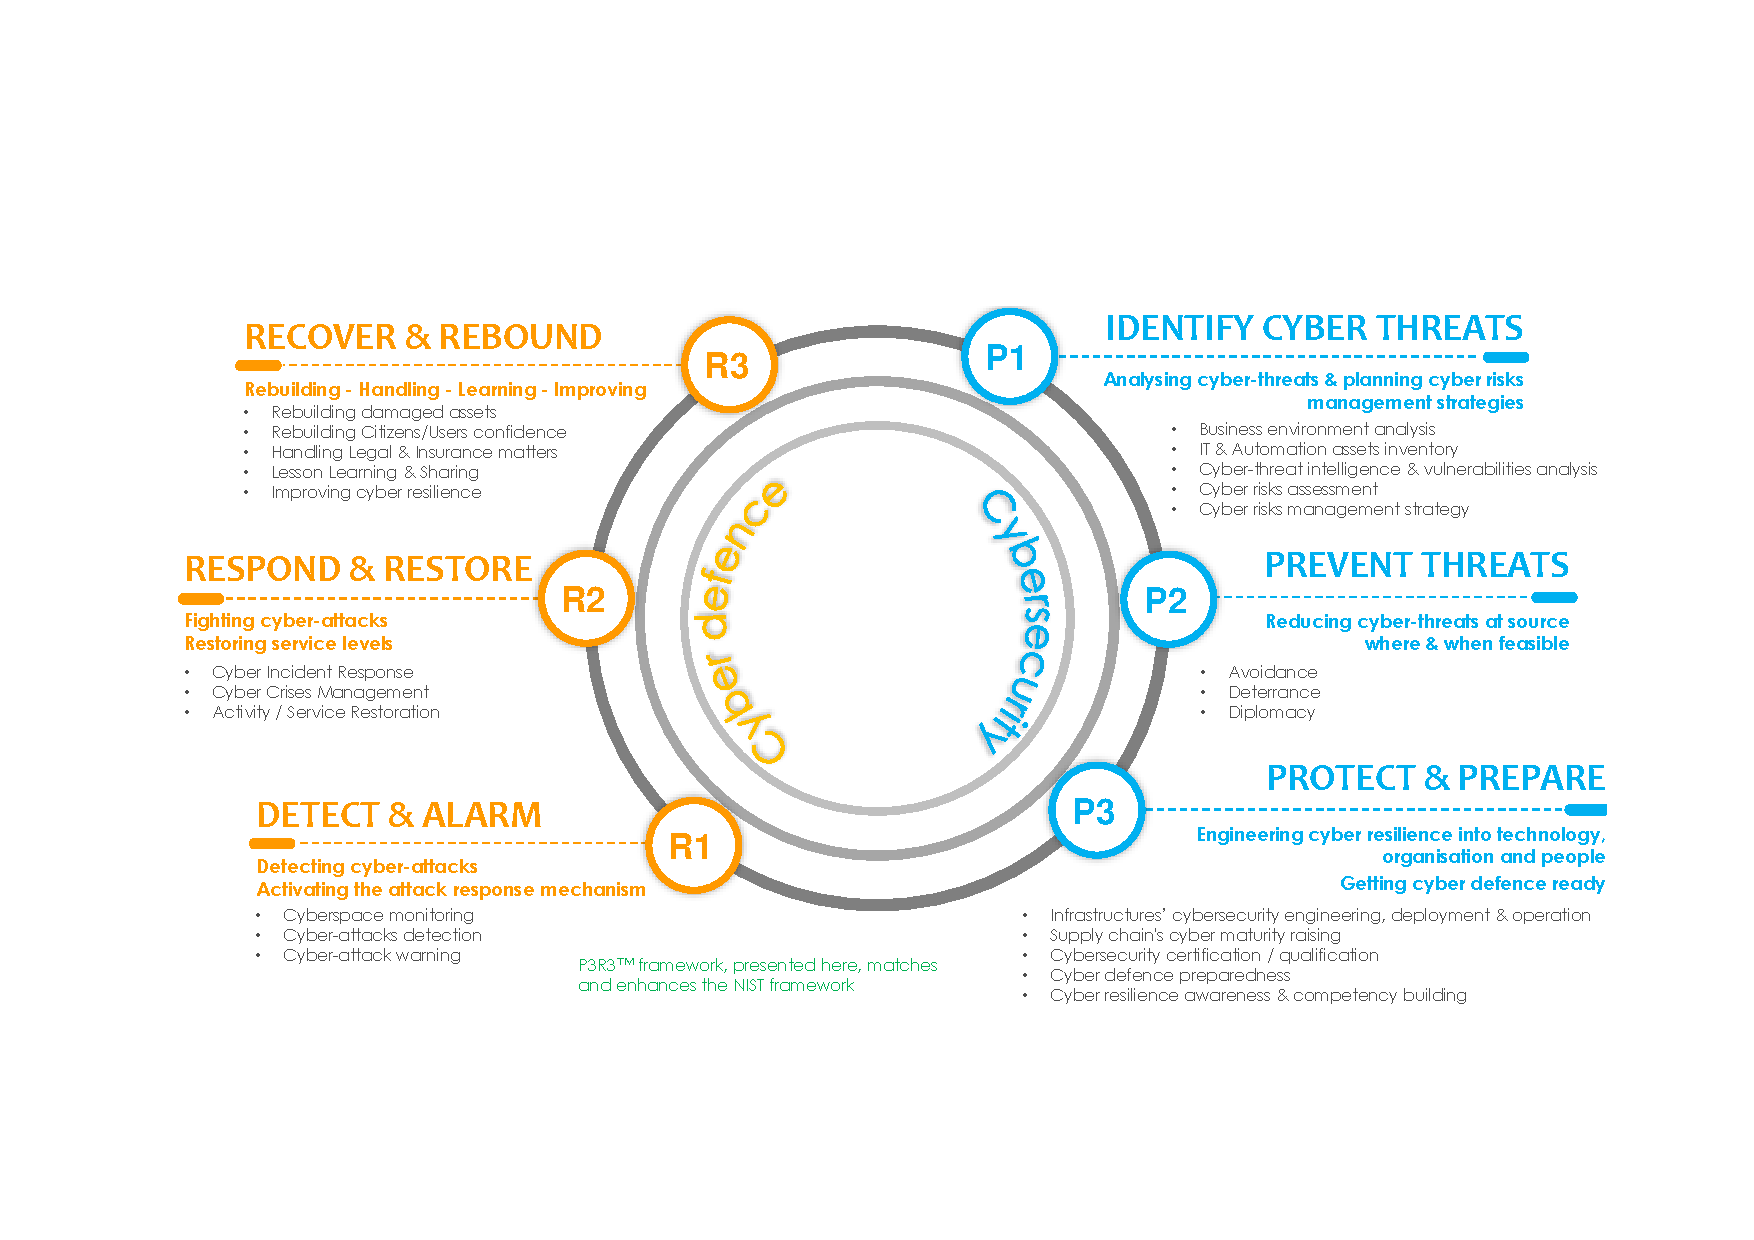
\includegraphics[width=\linewidth]{figures/P3R3.pdf}
  \caption{The P3R3 model for cyber resilience (from \autocite{Kott2023})}
  \label{fig:P3R3_model}
\end{figure}

\noindent
Cyber resilience essentially relies on a combination of detection and response to cyber threats. However, the emergence of increasingly rapid, distributed, and intelligent threats is challenging traditional approaches. We explore this in the following section, analyzing recent developments in the cyberattack landscape and the challenges associated with detecting and neutralizing them.


\section{Increasingly autonomous and distributed threats}\label{sec:evolution-threats}

In recent years, the cyber threat ecosystem has undergone a major transformation. The advent of agentic AI has enabled the emergence of faster, automated, adaptive attacks that operate in parallel not only on a single host, but across entire networks~\cite{Cohen2020}. Recent work shows that attackers are using \acn{LLM} to generate malware, create targeted phishing campaigns, and react autonomously to defense systems~\cite{AutoAttacker2024}. Such systems make it possible to launch distributed campaigns with great speed and efficiency~\cite{AgenticAIThreats2025}.

\subsection*{Limitations of traditional cyber defense approaches}

Traditional cyber defense mechanisms (based on centralized architectures, static signatures, or predefined rules) are now overwhelmed by this new generation of threats~\cite{Kott2023}~:
\begin{itemize}
  \item \textbf{Decision-making latency}: centralized detection causes critical delays, allowing certain attacks to occur before they are even identified and dealt with by cyberdefense teams;
  \item \textbf{Adaptive rigidity}: static rules cannot keep up with the evolution of attackers' methods;
  \item \textbf{Low resilience}: when an attack is detected, no immediate corrective action is taken. This delays system restoration and allows the consequences of the incident to worsen, thus limiting the effectiveness of the post-attack response.
\end{itemize}

These identified limitations highlight the need for a more agile, proactive, and intelligent paradigm in cyber defense. Recent studies identify the advent of AI-based attacks~\cite{Miles2018,AutoAttacker2024,Falong2025}, where malicious agents~:
\begin{itemize}

  \textbf{Automate} the search for vulnerabilities, the deployment of payloads, and exfiltration~;

  {itemize}
  \item \textbf{Automate} vulnerability scanning, payload deployment, and exfiltration;
  \item \textbf{Cooperate} by coordinating parallel attack vectors described in adversarial multi-agent models;
  \item \textbf{Exploit} adversarial ML techniques, generating forms of escape from usual detections (poisoning, prompt injection, etc.).
\end{itemize}

\subsection*{An autonomous approach to cyberdefense}

To address these threats, the emerging field of \acn{ACO}\index{ACO} seeks to develop systems capable of making complex decisions autonomously, taking into account the context, objectives to be achieved, and possible consequences of their actions, all in real time and with minimal or no human supervision~\cite{Vyas2023}. Early work in this field has focused mainly on architectures based on autonomous software agents, particularly within the framework of the \textit{IST-152} group of \acn{NATO}, which originated the concept of the \acn{AICA}\index{AICA} agent.
Such an agent is theorized as being capable of perceiving its local environment (through the analysis of logs, flows, or heuristics), make autonomous decisions based on rules or learning mechanisms, act locally (e.g., through filtering or isolation actions) without relying on permanent external control, and finally communicate with other agents or human operators to share indicators, intentions, or states.

In this context, the modular architecture \acn {MASCARA}~\cite{Theron2020MASCARA}\index{MASCARA}, illustrated in \autoref{fig:mascara}, was introduced to formalize the internal functioning of an agent \acn{AICA} by breaking down its activities into several specialized modules: log collection, anomaly detection, countermeasure selection, response application, etc. Based on this general architecture, it becomes possible to design a concrete instance adapted to a specific environment by modulating the number of components, their nature, and their interactions. Such adaptation allows the \acn{AICA} agent to respond precisely to the requirements of its deployment context and to guarantee protection {\em at the edge}, i.e., as close as possible to the resources to be defended, while optimizing performance in achieving cyberdefense objectives.

However, this architecture remains fundamentally monolithic and rigid. As it stands, it does not provide the necessary means of adaptation to cope with the unpredictable dynamics of a real operational environment, particularly in the context of distributed, complex, and highly interactive systems. This rigidity significantly limits the ability of an \acn{AICA} agent to respond to the emergence of new threats or to adjust to fluctuating environmental constraints.


\begin{figure}[h!]
  \centering
  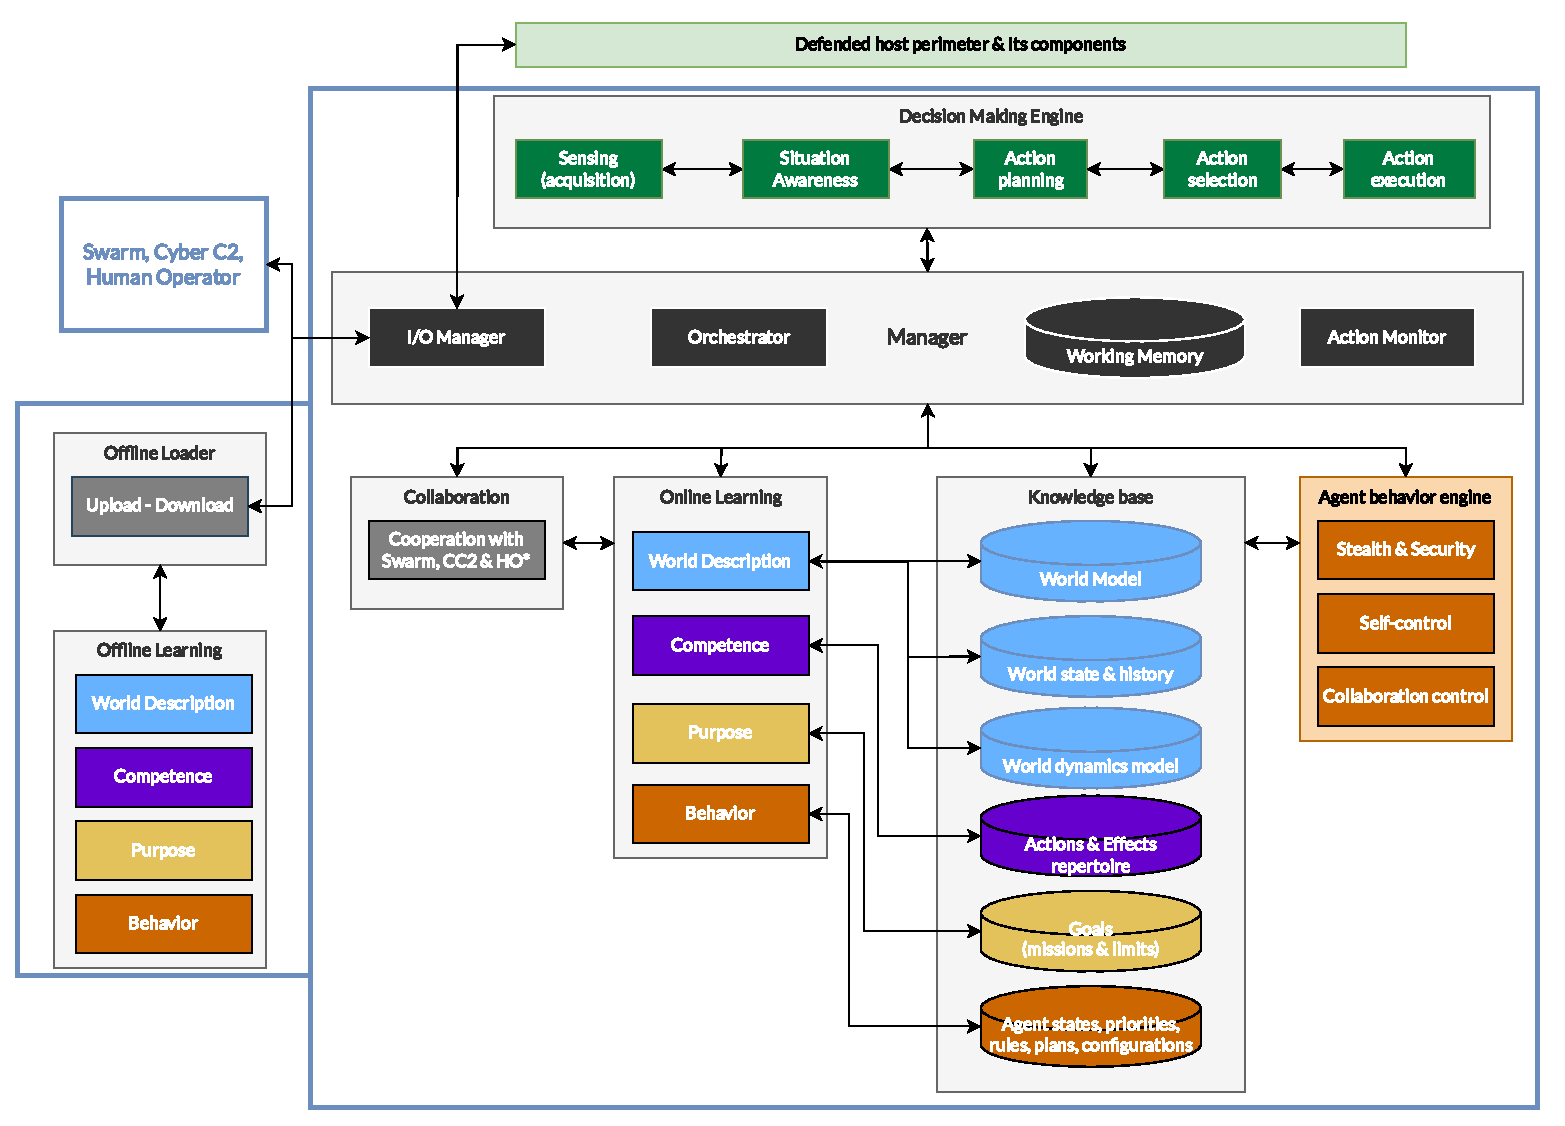
\includegraphics[width=\linewidth]{figures/MASCARA.pdf}
  \caption{Description of the MASCARA modular architecture (taken from \autocite{Kott2023})}
  \label{fig:mascara}
\end{figure}

\subsection*{Towards cooperative approaches}

The simple modular composition initially proposed is no longer sufficient to respond to the growing complexity of today's critical infrastructures. This requires the adoption of a distributed paradigm, in which several interconnected agents cooperate, self-organize, and dynamically reorganize themselves according to operational needs~\cite{Ferber1999, Gleizes2008}. With this in mind, the idea emerged to transform each module of the \acn {MASCARA} architecture into an autonomous agent responsible for performing a specific cyberdefense task. These micro-agents, interacting in a coordinated manner, would make it possible to better distribute responsibilities, strengthen the robustness of the system, and collectively achieve overall protection objectives.

The notion of granularity allows us to distinguish between micro-agents, each dedicated to a well-defined function, and so-called complete \acn{AICA} agents, capable of covering all the missions provided for by the model. In the rest of this manuscript, we will use the generic term \acn{AICA} agent to refer to these two types of agents, systematically specifying the functional scope concerned according to the context.

More generally, this distributed and cooperative approach is part of a systemic vision of cyberdefense, in which a set of autonomous agents interact within the network to ensure comprehensive, adaptive, and resilient security. This conceptual orientation is supported by several recent works in the emerging field of ACD~\cite{Vyas2023} (a subdomain of \acparen{ACO}) and forms an essential foundation for the developments presented in this manuscript.

For example, simulations have shown that teams of defensive agents are capable of outperforming a single agent in terms of network coverage and responsiveness, thanks to dynamic and distributed coordination~\cite{RLResilientCyberdefense2024}.
Platforms such as \acn{CybORG}~\cite{cage_challenge_3_announcement} also illustrate this trend, offering a simulated environment in which decentralized autonomous agents simultaneously defend a network against coordinated attacks.

The cooperative approach not only protects multiple hosts in parallel, but also detects synchronized attacks and dynamically adapts to changes in network topology. It thus lays the foundations for a distributed, proactive, and scalable cyberdefense, breaking with traditional defensive architectures.

\begin{figure}[h]
  \centering
  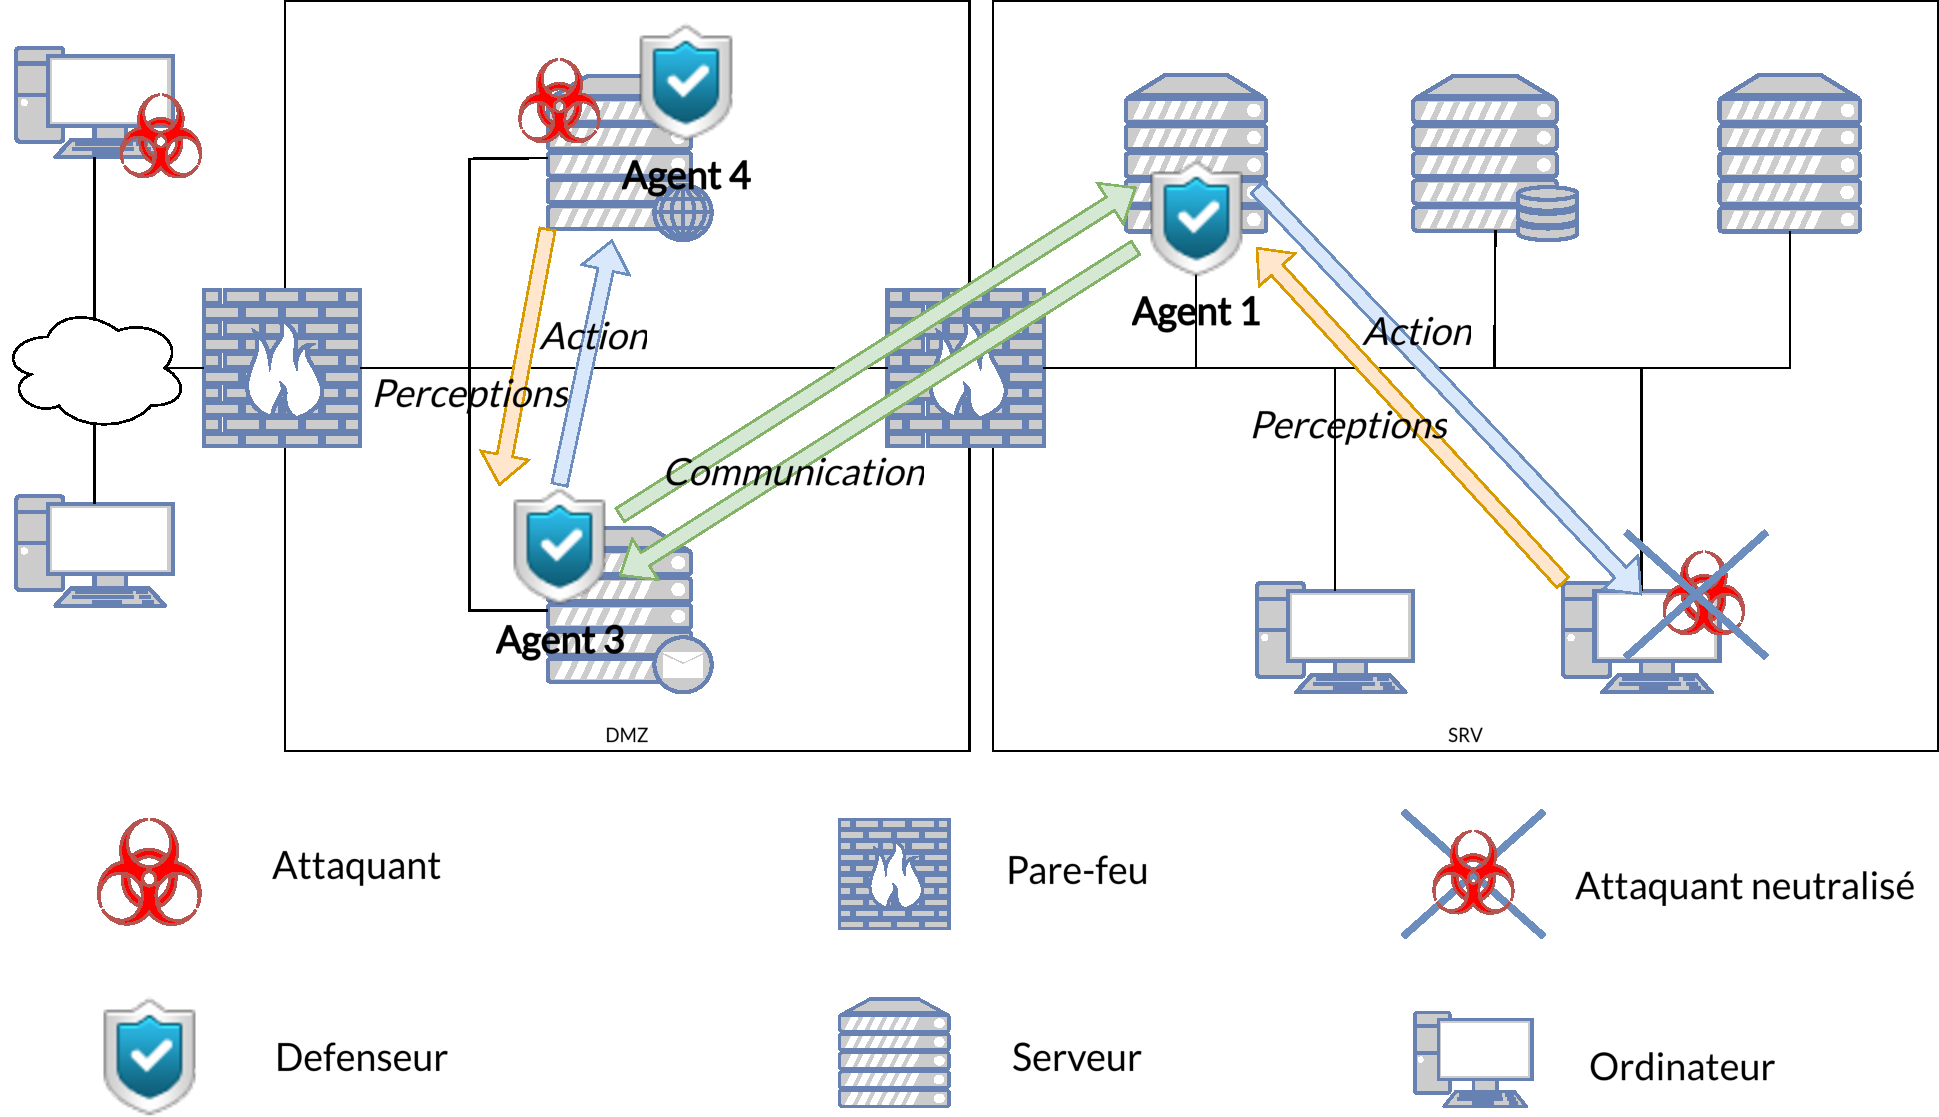
\includegraphics[width=\linewidth]{figures/infra_MAS_illustration.pdf}
  \caption{Schematic illustration of a Cyber Defense SMA in a toy enterprise infrastructure}
  \label{fig:distributed_sma}
\end{figure}

\noindent
Finally, it is in this context that the idea of a \acn{SMA} for cyber defense\index{SMA for cyber defense}, as illustrated in \autoref{fig:distributed_sma}, appears to be a promising generic alternative to existing centralized approaches. In the following section, we present the conceptual foundations of \acplu{SMA} with a view to designing a \acn{SMA} for cyber defense.

\section{The path to a multi-agent vision}\label {sec:sma-concepts}

\acplu{SMAs}\index{SMA} are a central paradigm of distributed \acn{AI}\index{distributed AI}. They enable the design of complex systems based on autonomous agents interacting in a shared environment. These agents can perceive, reason, decide, and act in a coordinated manner to solve collective problems~\cite{Ferber1999,Wooldridge2002}.

\subsection* {Fundamental definitions}

An \textbf{agent}\index{Agent} is an autonomous entity, physical or software-based, capable of perceiving its environment, making decisions, and acting to achieve objectives~\cite{Russell2010}. An \acn{SMA} brings together several of these agents, illustrated in \autoref{fig:sma_illustration}, which cooperate or interact within a generally dynamic and partially observable environment~\cite{Jennings1998,Shoham2007} . Each agent has a local observation zone (dotted disc) allowing it to perceive only part of the environment and other agents. Based on these partial observations, and according to strategies or policies (diagram at the top of the figure), it selects and executes \textbf{actions} directed at components of the environment (squares) or at other agents (solid arrows) . Agents can also \emph{exchange messages} (dashed arrows) in order to coordinate their behaviors. The exchange between one agent and another is considered to be the application of an action that modifies the second agent's upcoming observations. The overall objective (top right) represents a desired state of the environment that the agents seek to achieve collectively.

\begin{figure}[h]
  \centering
  \resizebox{\textwidth}{!}{%
    


\tikzset{every picture/.style={line width=0.75pt}} %set default line width to 0.75pt        

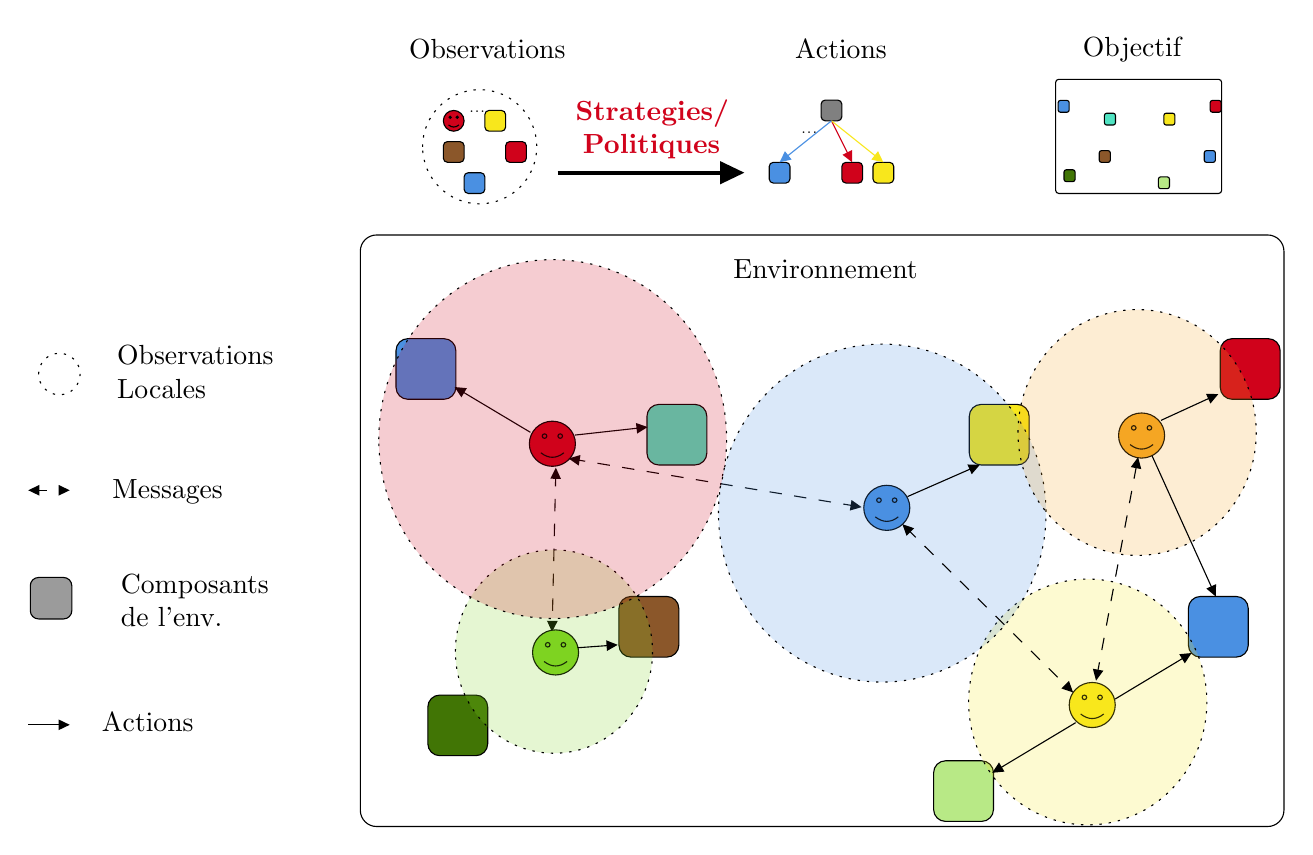
\begin{tikzpicture}[x=0.75pt,y=0.75pt,yscale=-1,xscale=1]
%uncomment if require: \path (0,1498); %set diagram left start at 0, and has height of 1498

%Rounded Rect [id:dp8571088761489256] 
\draw  [fill={rgb, 255:red, 255; green, 255; blue, 255 }  ,fill opacity=1 ] (195,482.84) .. controls (195,478.51) and (198.51,475) .. (202.84,475) -- (632.16,475) .. controls (636.49,475) and (640,478.51) .. (640,482.84) -- (640,752.16) .. controls (640,756.49) and (636.49,760) .. (632.16,760) -- (202.84,760) .. controls (198.51,760) and (195,756.49) .. (195,752.16) -- cycle ;
%Shape: Smiley Face [id:dp9608565483930217] 
\draw  [fill={rgb, 255:red, 208; green, 2; blue, 27 }  ,fill opacity=1 ] (276.44,575.59) .. controls (276.44,569.59) and (281.41,564.72) .. (287.53,564.72) .. controls (293.66,564.72) and (298.63,569.59) .. (298.63,575.59) .. controls (298.63,581.59) and (293.66,586.46) .. (287.53,586.46) .. controls (281.41,586.46) and (276.44,581.59) .. (276.44,575.59) -- cycle ; \draw  [fill={rgb, 255:red, 208; green, 2; blue, 27 }  ,fill opacity=1 ] (282.65,571.89) .. controls (282.65,571.29) and (283.15,570.81) .. (283.76,570.81) .. controls (284.37,570.81) and (284.87,571.29) .. (284.87,571.89) .. controls (284.87,572.49) and (284.37,572.98) .. (283.76,572.98) .. controls (283.15,572.98) and (282.65,572.49) .. (282.65,571.89) -- cycle ; \draw  [fill={rgb, 255:red, 208; green, 2; blue, 27 }  ,fill opacity=1 ] (290.2,571.89) .. controls (290.2,571.29) and (290.69,570.81) .. (291.31,570.81) .. controls (291.92,570.81) and (292.42,571.29) .. (292.42,571.89) .. controls (292.42,572.49) and (291.92,572.98) .. (291.31,572.98) .. controls (290.69,572.98) and (290.2,572.49) .. (290.2,571.89) -- cycle ; \draw   (281.99,579.94) .. controls (285.69,582.84) and (289.38,582.84) .. (293.08,579.94) ;
%Rounded Rect [id:dp759927621160896] 
\draw  [fill={rgb, 255:red, 80; green, 227; blue, 194 }  ,fill opacity=1 ] (333.1,562.39) .. controls (333.1,559.2) and (335.69,556.62) .. (338.87,556.62) -- (356.18,556.62) .. controls (359.37,556.62) and (361.95,559.2) .. (361.95,562.39) -- (361.95,580.06) .. controls (361.95,583.25) and (359.37,585.83) .. (356.18,585.83) -- (338.87,585.83) .. controls (335.69,585.83) and (333.1,583.25) .. (333.1,580.06) -- cycle ;
%Rounded Rect [id:dp3032709932069614] 
\draw  [fill={rgb, 255:red, 74; green, 144; blue, 226 }  ,fill opacity=1 ] (212.19,530.72) .. controls (212.19,527.54) and (214.77,524.95) .. (217.96,524.95) -- (235.26,524.95) .. controls (238.45,524.95) and (241.03,527.54) .. (241.03,530.72) -- (241.03,548.4) .. controls (241.03,551.58) and (238.45,554.17) .. (235.26,554.17) -- (217.96,554.17) .. controls (214.77,554.17) and (212.19,551.58) .. (212.19,548.4) -- cycle ;
%Straight Lines [id:da31697688905948296] 
\draw    (276.94,570.08) -- (243,549.8) ;
\draw [shift={(240.42,548.26)}, rotate = 30.86] [fill={rgb, 255:red, 0; green, 0; blue, 0 }  ][line width=0.08]  [draw opacity=0] (5.36,-2.57) -- (0,0) -- (5.36,2.57) -- cycle    ;
%Straight Lines [id:da15166297291059583] 
\draw  [dash pattern={on 4.5pt off 4.5pt}]  (289.15,590.12) -- (287.45,663.28) ;
\draw [shift={(287.38,666.28)}, rotate = 271.33] [fill={rgb, 255:red, 0; green, 0; blue, 0 }  ][line width=0.08]  [draw opacity=0] (5.36,-2.57) -- (0,0) -- (5.36,2.57) -- cycle    ;
\draw [shift={(289.22,587.12)}, rotate = 91.33] [fill={rgb, 255:red, 0; green, 0; blue, 0 }  ][line width=0.08]  [draw opacity=0] (5.36,-2.57) -- (0,0) -- (5.36,2.57) -- cycle    ;
%Straight Lines [id:da19030240516000207] 
\draw  [dash pattern={on 4.5pt off 4.5pt}]  (433.57,605.62) -- (298.31,583.17) ;
\draw [shift={(295.36,582.68)}, rotate = 9.42] [fill={rgb, 255:red, 0; green, 0; blue, 0 }  ][line width=0.08]  [draw opacity=0] (5.36,-2.57) -- (0,0) -- (5.36,2.57) -- cycle    ;
\draw [shift={(436.53,606.12)}, rotate = 189.42] [fill={rgb, 255:red, 0; green, 0; blue, 0 }  ][line width=0.08]  [draw opacity=0] (5.36,-2.57) -- (0,0) -- (5.36,2.57) -- cycle    ;
%Straight Lines [id:da12208855578128797] 
\draw    (298.42,571.41) -- (330.43,567.88) ;
\draw [shift={(333.41,567.55)}, rotate = 173.7] [fill={rgb, 255:red, 0; green, 0; blue, 0 }  ][line width=0.08]  [draw opacity=0] (5.36,-2.57) -- (0,0) -- (5.36,2.57) -- cycle    ;
%Shape: Smiley Face [id:dp017117759022491463] 
\draw  [fill={rgb, 255:red, 126; green, 211; blue, 33 }  ,fill opacity=1 ] (277.98,676.13) .. controls (277.98,670.13) and (282.94,665.26) .. (289.07,665.26) .. controls (295.2,665.26) and (300.16,670.13) .. (300.16,676.13) .. controls (300.16,682.13) and (295.2,687) .. (289.07,687) .. controls (282.94,687) and (277.98,682.13) .. (277.98,676.13) -- cycle ; \draw  [fill={rgb, 255:red, 126; green, 211; blue, 33 }  ,fill opacity=1 ] (284.19,672.44) .. controls (284.19,671.84) and (284.68,671.35) .. (285.3,671.35) .. controls (285.91,671.35) and (286.41,671.84) .. (286.41,672.44) .. controls (286.41,673.04) and (285.91,673.52) .. (285.3,673.52) .. controls (284.68,673.52) and (284.19,673.04) .. (284.19,672.44) -- cycle ; \draw  [fill={rgb, 255:red, 126; green, 211; blue, 33 }  ,fill opacity=1 ] (291.73,672.44) .. controls (291.73,671.84) and (292.23,671.35) .. (292.84,671.35) .. controls (293.45,671.35) and (293.95,671.84) .. (293.95,672.44) .. controls (293.95,673.04) and (293.45,673.52) .. (292.84,673.52) .. controls (292.23,673.52) and (291.73,673.04) .. (291.73,672.44) -- cycle ; \draw   (283.52,680.48) .. controls (287.22,683.38) and (290.92,683.38) .. (294.62,680.48) ;
%Rounded Rect [id:dp2729577267316856] 
\draw  [fill={rgb, 255:red, 65; green, 117; blue, 5 }  ,fill opacity=1 ] (227.53,702.44) .. controls (227.53,699.25) and (230.11,696.67) .. (233.3,696.67) -- (250.61,696.67) .. controls (253.8,696.67) and (256.38,699.25) .. (256.38,702.44) -- (256.38,720.11) .. controls (256.38,723.3) and (253.8,725.88) .. (250.61,725.88) -- (233.3,725.88) .. controls (230.11,725.88) and (227.53,723.3) .. (227.53,720.11) -- cycle ;
%Rounded Rect [id:dp9608207589356206] 
\draw  [fill={rgb, 255:red, 184; green, 233; blue, 134 }  ,fill opacity=1 ] (471.21,734.1) .. controls (471.21,730.92) and (473.79,728.33) .. (476.98,728.33) -- (494.29,728.33) .. controls (497.47,728.33) and (500.06,730.92) .. (500.06,734.1) -- (500.06,751.78) .. controls (500.06,754.96) and (497.47,757.55) .. (494.29,757.55) -- (476.98,757.55) .. controls (473.79,757.55) and (471.21,754.96) .. (471.21,751.78) -- cycle ;
%Rounded Rect [id:dp2532918382479751] 
\draw  [fill={rgb, 255:red, 248; green, 231; blue, 28 }  ,fill opacity=1 ] (488.39,562.39) .. controls (488.39,559.2) and (490.98,556.62) .. (494.16,556.62) -- (511.47,556.62) .. controls (514.66,556.62) and (517.24,559.2) .. (517.24,562.39) -- (517.24,580.06) .. controls (517.24,583.25) and (514.66,585.83) .. (511.47,585.83) -- (494.16,585.83) .. controls (490.98,585.83) and (488.39,583.25) .. (488.39,580.06) -- cycle ;
%Rounded Rect [id:dp46841976175690214] 
\draw  [fill={rgb, 255:red, 74; green, 144; blue, 226 }  ,fill opacity=1 ] (593.97,654.94) .. controls (593.97,651.75) and (596.55,649.17) .. (599.74,649.17) -- (617.04,649.17) .. controls (620.23,649.17) and (622.81,651.75) .. (622.81,654.94) -- (622.81,672.61) .. controls (622.81,675.8) and (620.23,678.38) .. (617.04,678.38) -- (599.74,678.38) .. controls (596.55,678.38) and (593.97,675.8) .. (593.97,672.61) -- cycle ;
%Rounded Rect [id:dp35096543230819477] 
\draw  [fill={rgb, 255:red, 208; green, 2; blue, 27 }  ,fill opacity=1 ] (609.31,530.72) .. controls (609.31,527.54) and (611.89,524.95) .. (615.08,524.95) -- (632.39,524.95) .. controls (635.58,524.95) and (638.16,527.54) .. (638.16,530.72) -- (638.16,548.4) .. controls (638.16,551.58) and (635.58,554.17) .. (632.39,554.17) -- (615.08,554.17) .. controls (611.89,554.17) and (609.31,551.58) .. (609.31,548.4) -- cycle ;
%Rounded Rect [id:dp37268226656767] 
\draw  [fill={rgb, 255:red, 139; green, 87; blue, 42 }  ,fill opacity=1 ] (319.6,654.94) .. controls (319.6,651.75) and (322.18,649.17) .. (325.37,649.17) -- (342.68,649.17) .. controls (345.87,649.17) and (348.45,651.75) .. (348.45,654.94) -- (348.45,672.61) .. controls (348.45,675.8) and (345.87,678.38) .. (342.68,678.38) -- (325.37,678.38) .. controls (322.18,678.38) and (319.6,675.8) .. (319.6,672.61) -- cycle ;
%Shape: Smiley Face [id:dp8112481576921686] 
\draw  [fill={rgb, 255:red, 245; green, 166; blue, 35 }  ,fill opacity=1 ] (560.32,571.63) .. controls (560.32,565.63) and (565.29,560.76) .. (571.41,560.76) .. controls (577.54,560.76) and (582.51,565.63) .. (582.51,571.63) .. controls (582.51,577.63) and (577.54,582.5) .. (571.41,582.5) .. controls (565.29,582.5) and (560.32,577.63) .. (560.32,571.63) -- cycle ; \draw  [fill={rgb, 255:red, 245; green, 166; blue, 35 }  ,fill opacity=1 ] (566.53,567.94) .. controls (566.53,567.34) and (567.03,566.85) .. (567.64,566.85) .. controls (568.25,566.85) and (568.75,567.34) .. (568.75,567.94) .. controls (568.75,568.54) and (568.25,569.02) .. (567.64,569.02) .. controls (567.03,569.02) and (566.53,568.54) .. (566.53,567.94) -- cycle ; \draw  [fill={rgb, 255:red, 245; green, 166; blue, 35 }  ,fill opacity=1 ] (574.08,567.94) .. controls (574.08,567.34) and (574.57,566.85) .. (575.19,566.85) .. controls (575.8,566.85) and (576.29,567.34) .. (576.29,567.94) .. controls (576.29,568.54) and (575.8,569.02) .. (575.19,569.02) .. controls (574.57,569.02) and (574.08,568.54) .. (574.08,567.94) -- cycle ; \draw   (565.87,575.98) .. controls (569.56,578.88) and (573.26,578.88) .. (576.96,575.98) ;
%Shape: Smiley Face [id:dp26692841414623936] 
\draw  [fill={rgb, 255:red, 248; green, 231; blue, 28 }  ,fill opacity=1 ] (536.54,701.46) .. controls (536.54,695.46) and (541.5,690.6) .. (547.63,690.6) .. controls (553.76,690.6) and (558.72,695.46) .. (558.72,701.46) .. controls (558.72,707.47) and (553.76,712.33) .. (547.63,712.33) .. controls (541.5,712.33) and (536.54,707.47) .. (536.54,701.46) -- cycle ; \draw  [fill={rgb, 255:red, 248; green, 231; blue, 28 }  ,fill opacity=1 ] (542.75,697.77) .. controls (542.75,697.17) and (543.24,696.68) .. (543.86,696.68) .. controls (544.47,696.68) and (544.97,697.17) .. (544.97,697.77) .. controls (544.97,698.37) and (544.47,698.86) .. (543.86,698.86) .. controls (543.24,698.86) and (542.75,698.37) .. (542.75,697.77) -- cycle ; \draw  [fill={rgb, 255:red, 248; green, 231; blue, 28 }  ,fill opacity=1 ] (550.29,697.77) .. controls (550.29,697.17) and (550.79,696.68) .. (551.4,696.68) .. controls (552.01,696.68) and (552.51,697.17) .. (552.51,697.77) .. controls (552.51,698.37) and (552.01,698.86) .. (551.4,698.86) .. controls (550.79,698.86) and (550.29,698.37) .. (550.29,697.77) -- cycle ; \draw   (542.08,705.81) .. controls (545.78,708.71) and (549.48,708.71) .. (553.18,705.81) ;
%Shape: Smiley Face [id:dp13683684589232226] 
\draw  [fill={rgb, 255:red, 74; green, 144; blue, 226 }  ,fill opacity=1 ] (437.56,606.46) .. controls (437.56,600.46) and (442.53,595.6) .. (448.65,595.6) .. controls (454.78,595.6) and (459.75,600.46) .. (459.75,606.46) .. controls (459.75,612.47) and (454.78,617.33) .. (448.65,617.33) .. controls (442.53,617.33) and (437.56,612.47) .. (437.56,606.46) -- cycle ; \draw  [fill={rgb, 255:red, 74; green, 144; blue, 226 }  ,fill opacity=1 ] (443.77,602.77) .. controls (443.77,602.17) and (444.27,601.68) .. (444.88,601.68) .. controls (445.5,601.68) and (445.99,602.17) .. (445.99,602.77) .. controls (445.99,603.37) and (445.5,603.86) .. (444.88,603.86) .. controls (444.27,603.86) and (443.77,603.37) .. (443.77,602.77) -- cycle ; \draw  [fill={rgb, 255:red, 74; green, 144; blue, 226 }  ,fill opacity=1 ] (451.32,602.77) .. controls (451.32,602.17) and (451.81,601.68) .. (452.43,601.68) .. controls (453.04,601.68) and (453.54,602.17) .. (453.54,602.77) .. controls (453.54,603.37) and (453.04,603.86) .. (452.43,603.86) .. controls (451.81,603.86) and (451.32,603.37) .. (451.32,602.77) -- cycle ; \draw   (443.11,610.81) .. controls (446.81,613.71) and (450.5,613.71) .. (454.2,610.81) ;
%Shape: Ellipse [id:dp20697299562525007] 
\draw  [fill={rgb, 255:red, 126; green, 211; blue, 33 }  ,fill opacity=0.2 ][dash pattern={on 0.84pt off 2.51pt}] (240.81,675.7) .. controls (240.81,648.64) and (262.07,626.7) .. (288.3,626.7) .. controls (314.52,626.7) and (335.79,648.64) .. (335.79,675.7) .. controls (335.79,702.76) and (314.52,724.7) .. (288.3,724.7) .. controls (262.07,724.7) and (240.81,702.76) .. (240.81,675.7) -- cycle ;
%Shape: Ellipse [id:dp5331145075645709] 
\draw  [fill={rgb, 255:red, 248; green, 231; blue, 28 }  ,fill opacity=0.2 ][dash pattern={on 0.84pt off 2.51pt}] (488.09,699.99) .. controls (488.09,667.29) and (513.78,640.78) .. (545.47,640.78) .. controls (577.17,640.78) and (602.86,667.29) .. (602.86,699.99) .. controls (602.86,732.7) and (577.17,759.21) .. (545.47,759.21) .. controls (513.78,759.21) and (488.09,732.7) .. (488.09,699.99) -- cycle ;
%Shape: Ellipse [id:dp1108681712787154] 
\draw  [fill={rgb, 255:red, 74; green, 144; blue, 226 }  ,fill opacity=0.2 ][dash pattern={on 0.84pt off 2.51pt}] (367.55,608.99) .. controls (367.55,564.02) and (402.88,527.57) .. (446.46,527.57) .. controls (490.04,527.57) and (525.37,564.02) .. (525.37,608.99) .. controls (525.37,653.96) and (490.04,690.41) .. (446.46,690.41) .. controls (402.88,690.41) and (367.55,653.96) .. (367.55,608.99) -- cycle ;
%Shape: Ellipse [id:dp35349211767213196] 
\draw  [fill={rgb, 255:red, 245; green, 166; blue, 35 }  ,fill opacity=0.2 ][dash pattern={on 0.84pt off 2.51pt}] (511.87,570.16) .. controls (511.87,537.46) and (537.56,510.95) .. (569.26,510.95) .. controls (600.95,510.95) and (626.65,537.46) .. (626.65,570.16) .. controls (626.65,602.86) and (600.95,629.38) .. (569.26,629.38) .. controls (537.56,629.38) and (511.87,602.86) .. (511.87,570.16) -- cycle ;
%Straight Lines [id:da868926834515953] 
\draw    (299.65,673.88) -- (315.99,672.69) ;
\draw [shift={(318.99,672.47)}, rotate = 175.83] [fill={rgb, 255:red, 0; green, 0; blue, 0 }  ][line width=0.08]  [draw opacity=0] (5.36,-2.57) -- (0,0) -- (5.36,2.57) -- cycle    ;
%Straight Lines [id:da7856168052805825] 
\draw    (458.62,601.05) -- (490.69,586.98) ;
\draw [shift={(493.44,585.77)}, rotate = 156.31] [fill={rgb, 255:red, 0; green, 0; blue, 0 }  ][line width=0.08]  [draw opacity=0] (5.36,-2.57) -- (0,0) -- (5.36,2.57) -- cycle    ;
%Straight Lines [id:da9445808525599552] 
\draw    (580.77,564.32) -- (605.66,552.9) ;
\draw [shift={(608.39,551.65)}, rotate = 155.36] [fill={rgb, 255:red, 0; green, 0; blue, 0 }  ][line width=0.08]  [draw opacity=0] (5.36,-2.57) -- (0,0) -- (5.36,2.57) -- cycle    ;
%Straight Lines [id:da12131692830119956] 
\draw    (558.67,698.58) -- (592.93,677.96) ;
\draw [shift={(595.5,676.42)}, rotate = 148.96] [fill={rgb, 255:red, 0; green, 0; blue, 0 }  ][line width=0.08]  [draw opacity=0] (5.36,-2.57) -- (0,0) -- (5.36,2.57) -- cycle    ;
%Straight Lines [id:da02866326716436185] 
\draw    (539.64,709.98) -- (502.01,732.57) ;
\draw [shift={(499.44,734.11)}, rotate = 329.03] [fill={rgb, 255:red, 0; green, 0; blue, 0 }  ][line width=0.08]  [draw opacity=0] (5.36,-2.57) -- (0,0) -- (5.36,2.57) -- cycle    ;
%Straight Lines [id:da3852011537026049] 
\draw  [dash pattern={on 4.5pt off 4.5pt}]  (458.31,616.46) -- (536.28,693.31) ;
\draw [shift={(538.42,695.42)}, rotate = 224.59] [fill={rgb, 255:red, 0; green, 0; blue, 0 }  ][line width=0.08]  [draw opacity=0] (5.36,-2.57) -- (0,0) -- (5.36,2.57) -- cycle    ;
\draw [shift={(456.17,614.35)}, rotate = 44.59] [fill={rgb, 255:red, 0; green, 0; blue, 0 }  ][line width=0.08]  [draw opacity=0] (5.36,-2.57) -- (0,0) -- (5.36,2.57) -- cycle    ;
%Straight Lines [id:da9204270310799157] 
\draw  [dash pattern={on 4.5pt off 4.5pt}]  (550.02,686.77) -- (569.17,585) ;
\draw [shift={(569.72,582.05)}, rotate = 100.65] [fill={rgb, 255:red, 0; green, 0; blue, 0 }  ][line width=0.08]  [draw opacity=0] (5.36,-2.57) -- (0,0) -- (5.36,2.57) -- cycle    ;
\draw [shift={(549.47,689.72)}, rotate = 280.65] [fill={rgb, 255:red, 0; green, 0; blue, 0 }  ][line width=0.08]  [draw opacity=0] (5.36,-2.57) -- (0,0) -- (5.36,2.57) -- cycle    ;
%Straight Lines [id:da9548969852220758] 
\draw    (576.47,581.42) -- (605.92,646.45) ;
\draw [shift={(607.16,649.18)}, rotate = 245.64] [fill={rgb, 255:red, 0; green, 0; blue, 0 }  ][line width=0.08]  [draw opacity=0] (5.36,-2.57) -- (0,0) -- (5.36,2.57) -- cycle    ;
%Shape: Ellipse [id:dp5345394122462545] 
\draw  [fill={rgb, 255:red, 208; green, 2; blue, 27 }  ,fill opacity=0.2 ][dash pattern={on 0.84pt off 2.51pt}] (203.9,573.33) .. controls (203.9,525.58) and (241.41,486.88) .. (287.68,486.88) .. controls (333.95,486.88) and (371.47,525.58) .. (371.47,573.33) .. controls (371.47,621.07) and (333.95,659.78) .. (287.68,659.78) .. controls (241.41,659.78) and (203.9,621.07) .. (203.9,573.33) -- cycle ;
%Rounded Rect [id:dp14561871899929513] 
\draw  [fill={rgb, 255:red, 155; green, 155; blue, 155 }  ,fill opacity=1 ] (36,644) .. controls (36,641.79) and (37.79,640) .. (40,640) -- (52,640) .. controls (54.21,640) and (56,641.79) .. (56,644) -- (56,656) .. controls (56,658.21) and (54.21,660) .. (52,660) -- (40,660) .. controls (37.79,660) and (36,658.21) .. (36,656) -- cycle ;
%Shape: Circle [id:dp8389216043634751] 
\draw  [dash pattern={on 0.84pt off 2.51pt}] (40,542) .. controls (40,536.48) and (44.48,532) .. (50,532) .. controls (55.52,532) and (60,536.48) .. (60,542) .. controls (60,547.52) and (55.52,552) .. (50,552) .. controls (44.48,552) and (40,547.52) .. (40,542) -- cycle ;
%Rounded Rect [id:dp1716372782625939] 
\draw  [fill={rgb, 255:red, 255; green, 255; blue, 255 }  ,fill opacity=1 ] (530,401.51) .. controls (530,400.68) and (530.68,400) .. (531.51,400) -- (608.49,400) .. controls (609.32,400) and (610,400.68) .. (610,401.51) -- (610,453.49) .. controls (610,454.32) and (609.32,455) .. (608.49,455) -- (531.51,455) .. controls (530.68,455) and (530,454.32) .. (530,453.49) -- cycle ;
%Rounded Rect [id:dp8384348356925067] 
\draw  [fill={rgb, 255:red, 80; green, 227; blue, 194 }  ,fill opacity=1 ] (553.51,417.41) .. controls (553.51,416.82) and (553.99,416.34) .. (554.57,416.34) -- (557.77,416.34) .. controls (558.35,416.34) and (558.83,416.82) .. (558.83,417.41) -- (558.83,420.96) .. controls (558.83,421.55) and (558.35,422.03) .. (557.77,422.03) -- (554.57,422.03) .. controls (553.99,422.03) and (553.51,421.55) .. (553.51,420.96) -- cycle ;
%Rounded Rect [id:dp32115157665477156] 
\draw  [fill={rgb, 255:red, 65; green, 117; blue, 5 }  ,fill opacity=1 ] (534.04,444.66) .. controls (534.04,444.07) and (534.52,443.59) .. (535.1,443.59) -- (538.3,443.59) .. controls (538.88,443.59) and (539.36,444.07) .. (539.36,444.66) -- (539.36,448.21) .. controls (539.36,448.8) and (538.88,449.28) .. (538.3,449.28) -- (535.1,449.28) .. controls (534.52,449.28) and (534.04,448.8) .. (534.04,448.21) -- cycle ;
%Rounded Rect [id:dp8306304589808061] 
\draw  [fill={rgb, 255:red, 184; green, 233; blue, 134 }  ,fill opacity=1 ] (579.52,448.07) .. controls (579.52,447.48) and (580,447) .. (580.59,447) -- (583.78,447) .. controls (584.37,447) and (584.84,447.48) .. (584.84,448.07) -- (584.84,451.62) .. controls (584.84,452.21) and (584.37,452.69) .. (583.78,452.69) -- (580.59,452.69) .. controls (580,452.69) and (579.52,452.21) .. (579.52,451.62) -- cycle ;
%Rounded Rect [id:dp36124132336547066] 
\draw  [fill={rgb, 255:red, 248; green, 231; blue, 28 }  ,fill opacity=1 ] (582.15,417.41) .. controls (582.15,416.82) and (582.63,416.34) .. (583.21,416.34) -- (586.41,416.34) .. controls (586.99,416.34) and (587.47,416.82) .. (587.47,417.41) -- (587.47,420.96) .. controls (587.47,421.55) and (586.99,422.03) .. (586.41,422.03) -- (583.21,422.03) .. controls (582.63,422.03) and (582.15,421.55) .. (582.15,420.96) -- cycle ;
%Rounded Rect [id:dp07486815562281168] 
\draw  [fill={rgb, 255:red, 74; green, 144; blue, 226 }  ,fill opacity=1 ] (601.62,435.41) .. controls (601.62,434.83) and (602.1,434.35) .. (602.68,434.35) -- (605.88,434.35) .. controls (606.46,434.35) and (606.94,434.83) .. (606.94,435.41) -- (606.94,438.97) .. controls (606.94,439.56) and (606.46,440.03) .. (605.88,440.03) -- (602.68,440.03) .. controls (602.1,440.03) and (601.62,439.56) .. (601.62,438.97) -- cycle ;
%Rounded Rect [id:dp30447435501798137] 
\draw  [fill={rgb, 255:red, 74; green, 144; blue, 226 }  ,fill opacity=1 ] (531.21,411.24) .. controls (531.21,410.66) and (531.69,410.18) .. (532.27,410.18) -- (535.47,410.18) .. controls (536.05,410.18) and (536.53,410.66) .. (536.53,411.24) -- (536.53,414.8) .. controls (536.53,415.39) and (536.05,415.86) .. (535.47,415.86) -- (532.27,415.86) .. controls (531.69,415.86) and (531.21,415.39) .. (531.21,414.8) -- cycle ;
%Rounded Rect [id:dp9375364402563595] 
\draw  [fill={rgb, 255:red, 208; green, 2; blue, 27 }  ,fill opacity=1 ] (604.45,411.24) .. controls (604.45,410.66) and (604.93,410.18) .. (605.51,410.18) -- (608.71,410.18) .. controls (609.29,410.18) and (609.77,410.66) .. (609.77,411.24) -- (609.77,414.8) .. controls (609.77,415.39) and (609.29,415.86) .. (608.71,415.86) -- (605.51,415.86) .. controls (604.93,415.86) and (604.45,415.39) .. (604.45,414.8) -- cycle ;
%Rounded Rect [id:dp7769696093588394] 
\draw  [fill={rgb, 255:red, 139; green, 87; blue, 42 }  ,fill opacity=1 ] (551.02,435.41) .. controls (551.02,434.83) and (551.5,434.35) .. (552.08,434.35) -- (555.28,434.35) .. controls (555.86,434.35) and (556.34,434.83) .. (556.34,435.41) -- (556.34,438.97) .. controls (556.34,439.56) and (555.86,440.03) .. (555.28,440.03) -- (552.08,440.03) .. controls (551.5,440.03) and (551.02,439.56) .. (551.02,438.97) -- cycle ;
%Straight Lines [id:da7689335282153781] 
\draw    (35,711) -- (52,711) ;
\draw [shift={(55,711)}, rotate = 180] [fill={rgb, 255:red, 0; green, 0; blue, 0 }  ][line width=0.08]  [draw opacity=0] (5.36,-2.57) -- (0,0) -- (5.36,2.57) -- cycle    ;
%Shape: Boxed Line [id:dp5305044082643576] 
\draw  [dash pattern={on 4.5pt off 4.5pt}]  (38,598) -- (52,598) ;
\draw [shift={(55,598)}, rotate = 180] [fill={rgb, 255:red, 0; green, 0; blue, 0 }  ][line width=0.08]  [draw opacity=0] (5.36,-2.57) -- (0,0) -- (5.36,2.57) -- cycle    ;
\draw [shift={(35,598)}, rotate = 0] [fill={rgb, 255:red, 0; green, 0; blue, 0 }  ][line width=0.08]  [draw opacity=0] (5.36,-2.57) -- (0,0) -- (5.36,2.57) -- cycle    ;
%Rounded Rect [id:dp4866637287235507] 
\draw  [fill={rgb, 255:red, 128; green, 128; blue, 128 }  ,fill opacity=1 ] (417,412) .. controls (417,410.9) and (417.9,410) .. (419,410) -- (425,410) .. controls (426.1,410) and (427,410.9) .. (427,412) -- (427,418) .. controls (427,419.1) and (426.1,420) .. (425,420) -- (419,420) .. controls (417.9,420) and (417,419.1) .. (417,418) -- cycle ;
%Rounded Rect [id:dp6679922716487737] 
\draw  [fill={rgb, 255:red, 74; green, 144; blue, 226 }  ,fill opacity=1 ] (392,442) .. controls (392,440.9) and (392.9,440) .. (394,440) -- (400,440) .. controls (401.1,440) and (402,440.9) .. (402,442) -- (402,448) .. controls (402,449.1) and (401.1,450) .. (400,450) -- (394,450) .. controls (392.9,450) and (392,449.1) .. (392,448) -- cycle ;
%Rounded Rect [id:dp6398718898903711] 
\draw  [fill={rgb, 255:red, 208; green, 2; blue, 27 }  ,fill opacity=1 ] (427,442) .. controls (427,440.9) and (427.9,440) .. (429,440) -- (435,440) .. controls (436.1,440) and (437,440.9) .. (437,442) -- (437,448) .. controls (437,449.1) and (436.1,450) .. (435,450) -- (429,450) .. controls (427.9,450) and (427,449.1) .. (427,448) -- cycle ;
%Straight Lines [id:da4441060393578834] 
\draw [color={rgb, 255:red, 208; green, 2; blue, 27 }  ,draw opacity=1 ]   (422,420) -- (430.66,437.32) ;
\draw [shift={(432,440)}, rotate = 243.43] [fill={rgb, 255:red, 208; green, 2; blue, 27 }  ,fill opacity=1 ][line width=0.08]  [draw opacity=0] (5.36,-2.57) -- (0,0) -- (5.36,2.57) -- cycle    ;
%Rounded Rect [id:dp08606049626209744] 
\draw  [fill={rgb, 255:red, 248; green, 231; blue, 28 }  ,fill opacity=1 ] (442,442) .. controls (442,440.9) and (442.9,440) .. (444,440) -- (450,440) .. controls (451.1,440) and (452,440.9) .. (452,442) -- (452,448) .. controls (452,449.1) and (451.1,450) .. (450,450) -- (444,450) .. controls (442.9,450) and (442,449.1) .. (442,448) -- cycle ;
%Straight Lines [id:da5780422632856335] 
\draw [color={rgb, 255:red, 248; green, 231; blue, 28 }  ,draw opacity=1 ]   (422,420) -- (444.66,438.13) ;
\draw [shift={(447,440)}, rotate = 218.66] [fill={rgb, 255:red, 248; green, 231; blue, 28 }  ,fill opacity=1 ][line width=0.08]  [draw opacity=0] (5.36,-2.57) -- (0,0) -- (5.36,2.57) -- cycle    ;
%Straight Lines [id:da6560295978621367] 
\draw [color={rgb, 255:red, 74; green, 144; blue, 226 }  ,draw opacity=1 ]   (422,420) -- (399.34,438.13) ;
\draw [shift={(397,440)}, rotate = 321.34] [fill={rgb, 255:red, 74; green, 144; blue, 226 }  ,fill opacity=1 ][line width=0.08]  [draw opacity=0] (5.36,-2.57) -- (0,0) -- (5.36,2.57) -- cycle    ;
%Rounded Rect [id:dp8389325005978227] 
\draw  [fill={rgb, 255:red, 139; green, 87; blue, 42 }  ,fill opacity=1 ] (235,432) .. controls (235,430.9) and (235.9,430) .. (237,430) -- (243,430) .. controls (244.1,430) and (245,430.9) .. (245,432) -- (245,438) .. controls (245,439.1) and (244.1,440) .. (243,440) -- (237,440) .. controls (235.9,440) and (235,439.1) .. (235,438) -- cycle ;
%Rounded Rect [id:dp11911600050294124] 
\draw  [fill={rgb, 255:red, 74; green, 144; blue, 226 }  ,fill opacity=1 ] (245,447) .. controls (245,445.9) and (245.9,445) .. (247,445) -- (253,445) .. controls (254.1,445) and (255,445.9) .. (255,447) -- (255,453) .. controls (255,454.1) and (254.1,455) .. (253,455) -- (247,455) .. controls (245.9,455) and (245,454.1) .. (245,453) -- cycle ;
%Rounded Rect [id:dp6632279611422938] 
\draw  [fill={rgb, 255:red, 248; green, 231; blue, 28 }  ,fill opacity=1 ] (255,417) .. controls (255,415.9) and (255.9,415) .. (257,415) -- (263,415) .. controls (264.1,415) and (265,415.9) .. (265,417) -- (265,423) .. controls (265,424.1) and (264.1,425) .. (263,425) -- (257,425) .. controls (255.9,425) and (255,424.1) .. (255,423) -- cycle ;
%Rounded Rect [id:dp1401057934464146] 
\draw  [fill={rgb, 255:red, 208; green, 2; blue, 27 }  ,fill opacity=1 ] (265,432) .. controls (265,430.9) and (265.9,430) .. (267,430) -- (273,430) .. controls (274.1,430) and (275,430.9) .. (275,432) -- (275,438) .. controls (275,439.1) and (274.1,440) .. (273,440) -- (267,440) .. controls (265.9,440) and (265,439.1) .. (265,438) -- cycle ;
%Shape: Smiley Face [id:dp8455919411140108] 
\draw  [fill={rgb, 255:red, 208; green, 2; blue, 27 }  ,fill opacity=1 ] (235,420) .. controls (235,417.24) and (237.24,415) .. (240,415) .. controls (242.76,415) and (245,417.24) .. (245,420) .. controls (245,422.76) and (242.76,425) .. (240,425) .. controls (237.24,425) and (235,422.76) .. (235,420) -- cycle ; \draw  [fill={rgb, 255:red, 208; green, 2; blue, 27 }  ,fill opacity=1 ] (237.8,418.3) .. controls (237.8,418.02) and (238.02,417.8) .. (238.3,417.8) .. controls (238.58,417.8) and (238.8,418.02) .. (238.8,418.3) .. controls (238.8,418.58) and (238.58,418.8) .. (238.3,418.8) .. controls (238.02,418.8) and (237.8,418.58) .. (237.8,418.3) -- cycle ; \draw  [fill={rgb, 255:red, 208; green, 2; blue, 27 }  ,fill opacity=1 ] (241.2,418.3) .. controls (241.2,418.02) and (241.42,417.8) .. (241.7,417.8) .. controls (241.98,417.8) and (242.2,418.02) .. (242.2,418.3) .. controls (242.2,418.58) and (241.98,418.8) .. (241.7,418.8) .. controls (241.42,418.8) and (241.2,418.58) .. (241.2,418.3) -- cycle ; \draw   (237.5,422) .. controls (239.17,423.33) and (240.83,423.33) .. (242.5,422) ;
%Shape: Circle [id:dp9393379743510656] 
\draw  [dash pattern={on 0.84pt off 2.51pt}] (225,432.5) .. controls (225,417.31) and (237.31,405) .. (252.5,405) .. controls (267.69,405) and (280,417.31) .. (280,432.5) .. controls (280,447.69) and (267.69,460) .. (252.5,460) .. controls (237.31,460) and (225,447.69) .. (225,432.5) -- cycle ;
%Straight Lines [id:da8347469557505708] 
\draw [line width=1.5]    (290,445) -- (312,445) -- (376,445) ;
\draw [shift={(380,445)}, rotate = 180] [fill={rgb, 255:red, 0; green, 0; blue, 0 }  ][line width=0.08]  [draw opacity=0] (11.61,-5.58) -- (0,0) -- (11.61,5.58) -- cycle    ;


% Text Node
\draw (419.14,491.63) node   [align=left] {Environnement};
% Text Node
\draw (115.53,541) node   [align=left] {Observations\\Locales};
% Text Node
\draw (335.35,421) node   [align=left] {\begin{minipage}[lt]{54.88pt}\setlength\topsep{0pt}
\begin{center}
\textbf{\textcolor[rgb]{0.82,0.01,0.11}{Strategies/}}\\\textbf{\textcolor[rgb]{0.82,0.01,0.11}{Politiques}}
\end{center}

\end{minipage}};
% Text Node
\draw (246,414) node [anchor=north west][inner sep=0.75pt]  [font=\Large] [align=left] {{\tiny ...}};
% Text Node
\draw (406,424) node [anchor=north west][inner sep=0.75pt]  [font=\Large] [align=left] {{\tiny ...}};
% Text Node
\draw (566.84,385.5) node   [align=left] {Objectif};
% Text Node
\draw (256.19,385.5) node   [align=left] {Observations};
% Text Node
\draw (426.6,385.5) node   [align=left] {Actions};
% Text Node
\draw (102.19,598.5) node   [align=left] {Messages};
% Text Node
\draw (92.6,709.5) node   [align=left] {Actions};
% Text Node
\draw (115.29,651) node   [align=left] {Composants\\de l'env.};


\end{tikzpicture}
  }
  \caption{Schematic example of an SMA}
  \label{fig:sma_illustration}
\end{figure}

\subsection*{Structural concepts: autonomy, coordination, and organization}

In the context of designing a \acn{SMA} for cyberdefense, three fundamental concepts structure our approach: autonomy, coordination, and organization.

\textbf{Autonomy}\index{Autonomy} refers to an agent's ability to perceive its environment, make decisions, and act without immediate external control~\cite{Russell2010, Boissier2003}. It implies a \textit{decoupling between agents} and a \textit{decentralization of the overall decision-making process}, with each agent being responsible for its own choices and actions. This autonomy can be expressed reactively (through a simple stimulus-response mechanism), deliberatively (through reasoning and planning), or in a hybrid form, combining these two dimensions~\cite {Georgeff1987}. In the context of cyber defense, autonomy allows an agent to detect an anomaly, assess the situation locally, and trigger a countermeasure without having to systematically report to a central authority.

\textbf{Coordination}\index{Coordination} refers to the mechanisms by which agents manage their interdependencies in order to cooperate effectively~\cite{Durfee2001, Jennings1996, Sandholm1999}. These mechanisms include negotiation, joint planning, task allocation, and social commitment. In a distributed cyberdefense environment, robust coordination is essential to avoid conflicts of intervention between agents, ensure consistency of responses, and dynamically distribute roles according to the situation.

The \textbf{organization}\index{Organisation} refers to the social structure in which agents operate: distribution of roles, allocation of responsibilities, management of dependencies and interactions. Two visions coexist in the literature~\cite{Picard2009reorganisation} and are summarized in \autoref{fig:auto_vs_topdown}. On the one hand, the organization can be explicit and reorganizable (top-down), where agents consciously manipulate a formal organizational specification, adapting roles or social relationships as needed. On the other hand, the organization can be emergent and self-organized (bottom-up), where agents interact locally, without any overall representation of the structure, and collectively bring about an organization via decentralized mechanisms~\cite{Heylighen1999, DiMarzoSerugendo2006}.

These two dynamics of organizational adaptation can be formalized by the following definitions. \textbf{Reorganization}\index{Reorganization} is an adaptation process triggered when the existing organization no longer allows the system's objectives to be met. It can be initiated by an agent or an external designer, and is based on the explicit manipulation of organizational primitives such as roles, dependencies, or interaction rules. Agents are then aware of the organization and able to modify it to ensure appropriate collective behavior~\cite{Picard2009reorganisation}.

Self-organization is an emergent, strictly endogenous process in which agents possess only local knowledge. By reacting to environmental pressure and interacting with their neighbors, they indirectly modify the overall configuration of the system (topology, neighborhoods, functional differentiation) without resorting to explicit modeling~\cite{Picard2009reorganisation}. {Picard2009reorganization}.

These two dynamics can be seen as two ends of a continuum. They embody two modalities of the same general process of organizational adaptation: detecting structural inadequacy and remedying it. While self-organization favors implicit, distributed, and bottom-up adaptation, reorganization relies on explicit, often planned mechanisms that may or may not be centralized.

\begin{figure}[h]
  \centering
  \resizebox{\textwidth}{!}{%
    \input{figures/organisation_mechanism}
  }
  \caption[Overview of the organization (from~\cite{Picard2009reorganization})]{Overview of the organization: (a) Emerging MAS~; (b) Coalition-based MAS~; (c) Agent-oriented engineering~; (d) Organization-oriented MAS (taken from~\cite{Picard2009reorganisation})}
  \label{fig:auto_vs_topdown}
\end{figure}

% \subsection*{Overview of research areas in \acn{MAS}}

% The field of \acn{SMA} is structured around several research areas:

% \begin{itemize}
% \item \textbf{Agent architectures}: reactive, cognitive, \acn{BDI}, hybrid~\cite{Georgeff1987}.
% \item \textbf{Coordination mechanisms}: auctions, negotiation, distributed planning, consensus~\cite{Sandholm1999,Durfee2001}.
% \item \textbf{Organizational models}: $\mathcal{M}OISE^+$~\cite{hubner2002moise,Hannoun2000}, OperA~\cite{Dignum2004}, \acn{AGR}~\cite{Ferber2004}.
% \item \textbf{Multi-agent learning}~: individual and collective learning in shared environments~\cite{Zhang2021}.
% \item \textbf{Safety, verification, and explainability}~: formal approaches to controlling emerging behaviors~\cite{Boella2006}.
% \item \textbf{Emergence and self-organization}: models inspired by biology or sociology to design robust and adaptive \acplu{MAS}~\cite{DiMarzoSerugendo2006,Heylighen1999}.
% \end{itemize}


\section{Designing a Cyberdefense MAS}\label{sec:problematique-sma}

MASAs, and in particular those inspired by the AICA model, offer a relevant framework for meeting these requirements. However, simply implementing autonomous agents is not enough: the entire design process must be rethought to ensure effective and sustainable cyber defense.
The central research question we address in this thesis can therefore be formulated as follows:

\begin{quote}
  \emph{How can we design a Cyberdefense \acn{SMA} capable of satisfactorily achieving its defense objectives, while self-organizing to dynamically adapt to environmental constraints and design requirements?}
\end{quote}

\medskip

This thesis aims to determine how to design a cyber defense \acn{SMA} capable of satisfactorily achieving its objectives, while dynamically adapting to its environment and design requirements. Cyberdefense objectives here correspond to the operational goals assigned to the system, such as intrusion detection, threat neutralization, service restoration, or continuous improvement of defensive capabilities, with reference to the P3R3 model~\cite{Theron2013P3R3} (detect, respond, restore) . Environmental constraints encompass all the limitations and characteristics of the SMA's operating context: network topology, available resources, threat dynamics, real-time requirements, security policies, etc. Finally, design requirements refer to the criteria and expectations set during the design of the \acn{SMA}, including distributed autonomy, resilience, explainability, performance measurability, regulatory compliance, and development and maintenance costs. The challenge is therefore to articulate these three dimensions in order to design a cyber defense \acn{SMA} that is effective, adaptable, and sustainable.

\medskip

\noindent
It is not just a question of equipping an \acn{SMA} with detection or response capabilities, but possibly of imagining a design framework where the organization of the agents themselves becomes a lever for efficiency and resilience~\cite{Picard2006, DiMarzoSerugendo2006} . This framework must meet a set of key criteria, presented below, which structure our scientific response to this question.

\subsection*{Criteria for evaluating \acn{SMA}s for cyber defense}\label{sec:criteria-evaluation}

Inspired by the challenges posed by the \textit{AICA IWG}~\footnotemark[3], we have defined a set of criteria, summarized in \autoref{tab:critere_aica}, describing the properties that a \acn {SMA} must satisfy in order to answer the overall research question.

\footnotetext[3]{In particular, research challenges related to \textit{Infrastructure Architecture and Engineering} and \textit{Individual \& Collective Decision Making}. See \url{https://www.aica-iwg.org/research-challenges/}}

\begin{table}[h!]
\centering
\caption{Grid of evaluation criteria for a Cyberdefense SMA}
\label{tab:criteria_aica}
\small
\renewcommand{\arraystretch}{1.2}
\begin{tabularx}{\textwidth}{
    >{\raggedright\arraybackslash\hsize=0.2\hsize}X
    >{\raggedright\arraybackslash\hsize=0.8\hsize}X
  }
  \hline
  \textbf{Criterion}            & \textbf{Summary of expectations}                                                                                                                                                                                                                                          \\
  \hline
  \textbf{C1 -- Autonomy}       & The \acn{SMA} must operate with minimal human intervention, whether during its design, implementation, operation, or shutdown. The goal is to reduce dependence on the operator by promoting self-organization and self-decision-making among agents.                     \\

  \textbf{C2 -- Performance}    & The \acn{SMA} must demonstrate sufficient performance to achieve the set objectives. This includes maximizing collective rewards and the ability to converge toward stable behaviors.                                                                                     \\

  \textbf{C3 -- Adaptation}     & The \acn{SMA} must be able to adjust to dynamic or uncertain environments. Agents must be able to maintain an acceptable level of performance in the face of disruptions, changes in objectives, or situations not encountered during training.                           \\

  \textbf{C4 -- Control}        & The \acn{SMA} must remain controllable at different levels: individual and collective. This implies the ability to impose or modify organizational specifications and to ensure the overall consistency of agents' behavior with these organizational specifications.     \\

  \textbf{C5 -- Explainability} & The \acn{SMA} must provide behaviors that are understandable to a human observer. The actions of agents and their coordination must be linkable to organizational specifications such as roles, missions, or objectives in order to interpret the defense logic deployed. \\
  \hline
\end{tabularx}
\end {table}

\noindent
\textbf{C1 - - Autonomy.}\index{Autonomy (C1)} \quad
Autonomy is a fundamental property expected of a cyber defense \acn{SMA}. It is not limited to an agent's ability to make decisions locally, but encompasses the entire life cycle of the \acn{SMA}, from its design and implementation to its operational execution and shutdown. An autonomous \acn{SMA} must therefore minimize dependence on human operators by promoting self-organization and decentralized decision-making. This requirement is particularly crucial in environments where reaction speed is critical and constant human supervision is impractical. Autonomy is therefore considered a necessary condition for increasing responsiveness, limiting the cognitive load on analysts, and ensuring continuity of operation in the face of rapid and distributed threats.

\medskip

\noindent
\textbf{C2 -- Performance.}\index{Performance (C2)} \quad
Performance refers to the ability of the \acn{SMA} to robustly and effectively achieve its assigned cyber defense objectives. It is manifested through the maximization of collective rewards obtained during experiments, but also through convergence towards stable and reproducible behaviors. A high-performing \acn{SMA} must be capable not only of detecting and neutralizing attacks, but also of maintaining satisfactory performance over repeated executions, without prolonged instability or behavioral oscillations. In this context, performance is evaluated not as a one-off success, but as a sustainable and generalizable property, guaranteeing the effectiveness of the system beyond a single scenario.

\medskip

\noindent
\textbf{C3 -- Adaptation.}\index{Adaptation (C3)} \quad
Adaptation reflects the ability of the \acn{SMA} to adjust its behavior in response to dynamic, uncertain, or unstable environments. It assumes that agents can absorb disturbances, respond to unprecedented situations, and quickly return to an acceptable level of functioning after a performance degradation. Adaptation also includes resilience to changes in objectives or operational conditions, such as variations in network topology, the emergence of new adversarial tactics, or fluctuating resource constraints. It is therefore considered an essential property for the sustainability of the system, ensuring that the \acn{SMA} does not remain stuck in a learned logic, but remains capable of maintaining operational effectiveness over time.

\medskip

\noindent
\textbf{C4 -- Control.}\index{Control (C4)} \quad
Control refers to the ability to guide and steer the behavior of the \acn{SMA}, whether at the individual or collective level. A controllable \acn{SMA} must allow for the imposition, modification, and monitoring of organizational specifications, such as roles, missions, or rules of interaction, while ensuring the overall consistency of observed behaviors. This criterion thus guarantees continuous alignment between design intentions and the actual dynamics of the system in operation. Control is a requirement for safety and trust, providing designers and operators with the means to limit undesirable behaviors and ensure that the \acn{SMA} acts in accordance with defined security policies. It thus establishes a necessary balance between local autonomy and external governance.

\medskip

\noindent
\textbf{C5 -- Explainability.}\index{Explainability (C5)} \quad
Explainability aims to ensure that the behaviors of the \acn{SMA}, whether individual or collective, can be understood and interpreted by a human observer. In the context of cyber defense, where transparency and trust are prerequisites for the adoption of automated solutions, it is essential that the actions of agents be linked to tangible organizational specifications, such as roles, missions, or intermediate objectives. Explainability is not limited to reporting on the action ex post, but also includes assessing the degree of similarity between the specified structures and those that actually emerge during execution. It thus constitutes a vector of readability and diagnosis, both strengthening operator confidence and improving the future design of \acplu{SMA} through a better understanding of emerging dynamics.

\section{Conclusion}
In summary, this chapter has laid the conceptual and methodological foundations of the thesis by identifying the issues, criteria, and tensions that structure the design of \acn{SMA} for cyber defense. It has highlighted the need for an integrated approach capable of reconciling performance, adaptation, control, and explainability, and has proposed formalizing the design as a constrained optimization problem. This reformulation has led to the decomposition of the problem into four fundamental sub-problems, each associated with a key activity in the design process. The rest of the manuscript will focus on exploring these sub-problems in greater depth, analyzing the obstacles identified in the literature and presenting the proposed contributions to address them, thus initiating the transition to the state of the art detailed in the following chapter.

\clearpage
\thispagestyle{empty}
\null
\newpage

\chapter{Towards Cyber Defense SMAs and their design}

% \acn{TODO}~: To be used to complete “Towards multi-agent approaches to Cyber Defense”
% % \usepackage{amsmath,amssymb,amsfonts}
% \usepackage{algorithmic}
% \usepackage{graphicx}
% \usepackage[inline]{enumitem}
% \usepackage{tabularx}
% \usepackage{caption}
% \usepackage[T2A,T1]{fontenc}
% \usepackage[french]{babel}
% \captionsetup{font=it}
% \usepackage{ragged2e}
% \usepackage{hyperref}
% \usepackage{footmisc}
% \usepackage{booktabs}
% \usepackage{smartdiagram}
% \usepackage{textcomp}
% \usepackage{xcolor}
% \def\BibTeX{{\rm B\kern-.05em{\sc i\kern-.025em b}\kern-.08em
%     T\kern-.1667em\lower.7ex\hbox{E}\kern-.125emX}}
% \usepackage{cite}

% \usepackage{etoolbox}
% \patchcmd{\thebibliography}{\section*{\refname}}{}{}{}

% \setlength{\extrarowheight}{2.5pt}


\section{Introduction}

% Le contexte
% Alors que de plus en plus de réseaux et d'appareils connectés sont utilisés, en particulier dans l'<<~Internet of Things~>> (IoT) et l'<<~Internet of Battle Things~>> (IoBT), le besoin de leur propre sécurité est devenu un défi très important. Les systèmes tels que les capteurs sans fil ou les véhicules autonomes ont une surface d'attaque accrue, car ils offrent de nouveaux vecteurs d'attaque pour corrompre, détruire et propager de nouvelles cyber-attaques sur les réseaux connectés.
%\cite{ccdc_army_research_laboratory_internet_2017}.


Le développement de l'<<~Internet of Things~>> et de l'<<~Internet of Battle Things~>>  a entrainé une augmentation de la surface d'attaque des systèmes en réseau permettant à des attaquants de s'y introduire en ciblant les nœuds les plus faiblement défendus. Tenant compte de ce contexte, le groupe de travail <<~AICA IWG~>>\footnote{Ce groupe de travail (voir \url{https://www.aica-iwg.org/}) s'appuie sur les résultats du \textit{Research Task Group IST-152} de l'OTAN qui a travaillé sur le concept des <<~Intelligent, Autonomous and Trusted Agents for Cyber Defense and Resilience~>>.} a poursuivi le développement des travaux concernant l'agent AICA (Autonomous Intelligent Cyber-defence Agent).
Un agent est par définition une entité autonome capable de percevoir son environnement local grâce à des capteurs, et d’agir sur cet environnement à l'aide d'effecteurs\cite{russell1995modern}.
L'agent AICA doit pouvoir être déployé sur un système hôte pour détecter, identifier et caractériser des anomalies/attaques, élaborer et piloter l’exécution de contre-mesures et dialoguer avec l'extérieur. À cette fin, il est conçu comme proactif, discret et capable d’apprendre.

% \noindent



L'agent AICA peut être vu comme un Système Multi-Agent (SMA). Le paradigme multi-agent offre des moyens de gérer l'ouverture, le passage à l'échelle et l'autonomie du système hôte en déléguant différents aspects de la cyber-défense à différents agents. L'agent AICA  est alors un système collectif décentralisé et distribué d'agents cyber-défenseurs déployés au plus près des composants du système\cite{ieeesp_KottT20}.
%Évitant l'écueil d'un point de défaillance unique, ils contribuent aussi à opposer plusieurs couches de cyber-défense à un éventuel cyber-attaquant.

Concevoir un tel SMA, nécessite de porter une attention particulière à son organisation. L'objectif de cet article est de discuter des mécanismes organisationnels d'un SMA de cyberdéfense.
% Cet article aborde des mécanismes organisationnels disponibles pour concevoir un SMA qui répond à des objectifs de cyber-défense ainsi qu'aux contraintes du système hôte de déploiement.
% Notre intérêt porte principalement sur la protection des systèmes en réseau dont les nœuds peuvent héberger des agents.% aussi bien sur des réseaux mobiles que sur des réseaux fixes.
% La recherche de recommandations et/ou pistes de conception pour ce SMA s'appuie sur une revue des différentes organisations disponibles avec leurs objectifs de cyber-défense et systèmes hôtes associés.
% Structure & Méthode
La section II introduit un état de l'art de SMA existants assurant la cyber-défense sur leur système hôte. La section III identifie les verrous théoriques et techniques potentiels vers la conception d'un SMA de cyber-défense auto/ré-organisé et propose des préconisations.

% REMARQUE : plutôt que edt mettre uniquement "Travaux liés"
\section{\'Etat de l'art}

\subsection{Vers des systèmes multi-agents de cyber-défense}


% % Expliquer à quels défis de sécurité nous devons initialement faire face...
% Le monde du cyber
% % dans lequel opère tout système fournissant une couverture de sécurité
% rassemble une grande variété de définitions et de termes issus de plusieurs domaines\cite{bjorck2015cyber}. Le terme \textbf{cyber} fait référence à toutes les activités liées à une utilisation offensive ou défensive du cyberespace\cite{nocetti2018darkening}.

Nous inscrivant dans le prolongement des travaux menés dans le cadre de l'AICA IWG, nous considérons la \textbf{cyber-sécurité} comme l'ensemble des activités  consistant à se protéger de façon préventive contre les cyber-attaques\cite{theron_autonomous_2021}.


Nous désignons par \textbf{cyber-défense}  l'ensemble des activités entreprises lorsqu'une cyber-attaque est détectée et qu'il faut réagir. Ces activités sont décrites dans le cadre du <<~P3R3 Resilience Engineering Framework~>>\cite{Theron2013P3R3} et sont regroupées en trois fonctions de cyber-défense :

\noindent
\textit{\textbf{R1 - Detect and alarm}} : détection des cyber-attaques  et déclenchement des mécanismes de réponse; %Cela couvre également la surveillance du système à défendre et l'avertissement d'éventuelles cyber-attaques.

\noindent
\textit{\textbf{R2 - Respond and restore}} : mise en œuvre et suivi des réponses apportées aux cyber-attaques et l restauration des niveaux de services/activités minimaux. La gestion de la crise provoquée par l'attaque est au cœur de cette fonction;

\noindent
\textit{\textbf{R3 - Recover and rebound}} : rétablissement des parties endommagées du système à défendre et traitement final des conséquences. Ce point inclut une phase d'apprentissage permettant l'amélioration du système de cyber-défense.

% \begin{figure}[ht!]
%     \centering
%     \smartdiagramset{back arrow disabled=true}
%     \smartdiagram[flow diagram:horizontal]{\textbf{(R1)} Detecter \& Alarmer, \textbf{(R2)} Répondre \& Restaurer, \textbf{(R3)} Rétablir \& Rebondir}
%     \caption{Cadre fondamental de travail pour la cyber-défense (tiré de \cite{Theron2013P3R3})}
%     \label{fig:framework_r3}
% \end{figure}

%(contrecarrer une cyber-attaque après qu'elle a réussi)

%(en prévention d'une cyber-attaque) \cite{theron_autonomous_2021}.
% Les deux sont importants pour assurer la \textbf{cyber résilience}\cite{theron_autonomous_2021}.
% Nous choisissons d'inclure les objectifs de cyber-défense, de cyber-sécurité et de cyber résilience dans le même terme d'\textbf{objectif de cyber-défense}.

Nous appelons \textbf{objectifs de cyber-défense}, tous les objectifs impliquant la mise en œuvre d'une ou plusieurs des %\old{activités} 
fonctions de cyber-défense.

% qui ont pour finalité de garantir des critères de sécurité sans perturber la productivité du système défendu dans le cas où une cyber-attaque a eu lieu\cite{keyser2018information}. Sur la base de la norme ISO 25010, des triades CIA (Confidentiality, Intégrity, Availability) et AAA (Authentication, Availability, Accountability), nous avons choisi la recherche de la confidentialité, l'intégrité, la disponibilité, la responsabilité et la non-répudiation comme cadre initial fondamental de nos objectifs de cyber-défense.%\cite{iso25010}.

% Un tel système repose sur la répartition de la responsabilité de la sécurité entre plusieurs agents. Ces agents peuvent être conçus pour surveiller différents aspects du système, tels que le trafic réseau, l'activité des utilisateurs et les journaux système, et pour prendre les mesures appropriées lorsque des cyber-menaces sont détectées.
% Un SMA peut inclure des agents chargés d'identifier et de bloquer le trafic malveillant, des agents qui surveillent l'activité des utilisateurs et détectent les comportements suspects, et des agents qui analysent les journaux système et alertent les administrateurs des problèmes de sécurité potentiels.
% L'utilisation de plusieurs agents peut améliorer la sécurité du système hôte de plusieurs façons. Premièrement, cela permet une approche plus globale de la sécurité, car différents agents peuvent se concentrer sur différents aspects du système. Deuxièmement, cela peut réduire le risque d'un point de défaillance unique, car la défaillance d'un agent ne compromettra pas nécessairement la sécurité de l'ensemble du système. Enfin, l'utilisation de plusieurs agents peut rendre plus difficile pour un attaquant de compromettre le système, car il devrait contourner plusieurs couches de cyber-défense.

% \textbf{La confidentialité} est la capacité d'un système à ne pas rendre les données accessibles aux personnes non autorisées\cite{noauthor_glossaire_nodate} ;
% % (via le chiffrement, les règles et politiques de contrôle d'accès, l'authentification, la gestion des autorisations qui limite les actions possibles selon des règles).

% \textbf{L'intégrité} est la capacité d'un système à se protéger des modifications non autorisées\cite{noauthor_glossaire_nodate} ;
% % (via les sauvegardes, les sommes de contrôle, le contrôle de version, les journaux de données, les erreurs de données et les codes de correction).

% \textbf{Disponibilité} est "la capacité d'un élément/entité à pouvoir exécuter une fonction requise dans des conditions données, à un moment donné ou pendant un intervalle de temps donné, en supposant que les ressources externes nécessaires sont fournies"\cite{ afnor_norme_nodate} ;
% % (au travers des protections physiques, de la redondance et du plan de continuité et de reprise des données).

% \textbf{Non-répudiation} qui est la capacité d'un système à prouver qu'une action a bien été appliquée\cite{25010_2011} ;

% \textbf{Responsabilité} qui est la capacité d'un système à retracer les actions avec ceux qui sont derrière elles\cite{1400-1700_isoiec_nodate}.
% elle inclut la \textbf{traçabilité} car c'est "la capacité à suivre la vie d'une exigence, depuis ses origines, en passant par son développement, ses spécifications, son déploiement et son utilisation"\cite {gotel_analysis_1994} ; et \textbf{authenticité} qui est la capacité d'un système à apporter la preuve de son identité\cite{noauthor_glossaire_nodate}.


% montrant que ces problèmes sont résolus par la sécurité collaborative...
% \subsection{cyber-sécurité collaborative via des SMA}


% la sécurité collaborative qu'on défini comme...
% notion de sécurité collaborative sujette à caution...
%\old{[[Supprimé]]La littérature fournit le concept de \textbf{sécurité collaborative} impliquant plusieurs parties techniques et non techniques dans le processus d'identification, de prévention et de réponse aux cyber-menaces sur des infrastructures\cite{meng2015collaborative}.}
% Cela implique, entre autres, le partage d'informations, de ressources et d'expertise afin d'améliorer l'efficacité et l'efficience des mesures de cyber-sécurité et cyber-défense\cite{meng2015collaborative}.

% technique : logiciel et matériel
% SOC central insuffisant...
%\old{[[Supprimé:]]Inspirés par ce paradigme, nous définissons la \textbf{cyber-défense collaborative} comme la poursuite d'objectifs de cyber-défense par plusieurs entités logicielles réagissant aux cyber-attaques ciblant un système vu comme un réseau de nœuds.}
% todo : expliciter la finalité

Dans un \textbf{SMA de cyber-défense}, plusieurs agents atteignent un objectif global de cyber-défense par un comportement collectif résultant de la réalisation de sous-objectifs individuels et/ou de mécanismes locaux\cite{jamont2015meeting}. Des exemples de tels sous-objectifs pourraient être la détection des intrusions, la mise en œuvre d'un plan de récupération, la restauration d'une image, redirection des ports\dots

% Selon la référence \cite{boissier2004caractéristiques}, les SMA sont :
% autonome (la prise de décision ne dépend pas d'une entité externe) ; répartis (les connaissances ou les tâches sont réparties dans chaque agent) ; décentralisé (la responsabilité d'atteindre un objectif est confiée à tous les agents) ; situé dans l'environnement (espace commun où interagissent les agents \cite{odell2002modeling}) ; permettre des interactions entre agents (action réciproque de deux ou plusieurs entités\cite{noauthor_interaction_nodate} pouvant conduire à des stratégies de coopération, collaboration, compétition, négociation entre les agents) en utilisant la communication (assurer une cohérence globale malgré la décentralisation en utilisant un langage grammaticalement structuré, utiliser d'un protocole spécifique, utilisation d'un espace commun ou "tableau noir"); montrant l'émergence (résultat du comportement des agents individuels à travers leurs interactions\cite{di2005self}) ; et avoir une organisation (en tant que modèle global éventuellement défini a priori ou en tant que phénomène émergent\cite{salvador2019multi}).


\subsection{Mécanismes organisationnels dynamiques}

L'autonomie de fonctionnement du SMA de cyber-défense, obtenue  en déléguant aux agents certaines missions % avec peu d'interventions directes, 
est une réponse face aux charges de travail des équipes cyber et à la rapidité des cyber-attaques\cite{ieeesp_KottT20}.
Un tel SMA doit modifier sa structure et les relations entre ses agents pour continuellement s'adapter à son environnement \cite{theron_autonomous_2021}.
%La réorganisation et l'auto-organisation sont alors des mécanismes clés  \cite{picard2009reorganisation}.

% De plus, comme discuté dans \cite{theron_autonomous_2021}, nous avançons l'hypothèse que les mécanismes d'organisation assurant la sécurité sont susceptibles de nécessiter un bon niveau de représentation et de conscience de l'environnement pour un processus de prise de décision et d'apprentissage complexe précis.

% La \textbf{réorganisation} est définie comme un processus descendant imposant une organisation (vue comme une entité distincte) aux agents. Ces mécanismes de réorganisation sont inclus dans l'Organisation-Centered Point Of View (OCPV)\cite{picard2009reorganisation}. Dans l'OCPV, la sécurité globale est une tâche commune partagée par tous les agents à travers leur organisation. Il s'avère être un moyen de basculer entre plusieurs organisations éprouvées qui semblent adaptées dans des circonstances données.
% À une faible conscience environnementale/organisationnelle, une organisation basée sur OCPV peut être codée en dur en tant que règles de sécurité à suivre dans les agents eux-mêmes.
% Avec un niveau de conscience environnementale et/ou organisationnelle plus élevée, une organisation basée sur l'OCPV est partagée comme une représentation globale (topologie) par tous les agents qui peuvent la modifier directement par des processus sociaux.
% Selon \cite{picard2009reorganisation}, de tels SMA sont dits "\textbf{organization oriented}". Les rôles et cahiers des charges qui composent l'organisation sont à faire évoluer par les agents eux-mêmes (ou des entités extérieures) lorsque l'organisation n'est pas adaptée en travaillant directement sur des schémas de coopération et d'organisation \cite{picard2009reorganisation}.

% \textbf{L'auto-organisation} est définie comme un processus ascendant où l'organisation résulte des interactions et des actions locales des agents comme un phénomène émergent. Les mécanismes d'auto-organisation appartiennent à l'Agent-Centered-Point-Of-View (ACPV)\cite{picard2009reorganisation}. Dans l'ACPV, la sécurité globale résulte des actions de sécurité locales et des interactions pair à pair entre les agents. C'est un moyen efficace de faire face aux cyber-menaces sans avoir besoin d'un contrôle ou d'un guidage central.
% À une faible conscience environnementale/organisationnelle, une organisation basée sur l'ACPV est conçue pour réagir au déclenchement de combinaisons d'événements de sécurité pour appliquer des actions cartographiées. Il convient de noter que la notion récurrente d'"intelligence en essaim" est incluse dans ce cas car il n'y a aucune connaissance de l'organisation pour les agents.
% Avec un niveau de conscience environnementale et/ou organisationnelle plus élevée, une organisation basée sur l'ACPV tire parti de la représentation locale intégrée de l'environnement direct de l'agent (agents cyber-défenseurs voisins, nœuds de réseau découverts, processus en cours d'exécution, etc.) pour un processus cognitif.
% Selon \cite{picard2009reorganisation}, de tels SMA sont dits "\textbf{coalition based}". Les dépendances/relations inter-agents sont modifiées par les agents eux-mêmes en raison d'une inadéquation en modifiant les schémas de coopération ou indirectement l'organisation.

En considérant un point de vue centré organisation, la cyber-défense globale est une tâche commune partagée par tous les agents à travers leur organisation. La \textbf{ré-organisation} est un moyen de basculer entre plusieurs organisations éprouvées qui semblent adaptées dans des circonstances données\cite{picard2009reorganisation}.

En considérant un point de vue centré agent, l’\textbf{auto-organisation} est définie comme un processus ascendant où l’organisation émerge des interactions et des actions locales des agents. La cyber-défense globale résulte alors des actions de cyber-défense locales et des interactions pair à pair entre les agents\cite{picard2009reorganisation}. L'auto-organisation semble être un des moyens à mobiliser pour faire face aux cyber-menaces en évitant les écueils d'un contrôle centralisé.



\begin{table*}[t!]

    \caption{Un aperçu de quelques organisations et des environnement hôtes utilisés dans les SMA de cyber-défense étudiés}

    \begin{tabularx}{\linewidth}{
            >{\raggedright\arraybackslash\hsize=.3\hsize}X
            >{\raggedright\arraybackslash\hsize=.6\hsize}X
            >{\raggedright\arraybackslash\hsize=.6\hsize}X
            >{\raggedright\arraybackslash\hsize=.6\hsize}X
            % >{\raggedright\arraybackslash}X
            >{\raggedright\arraybackslash\hsize=.2\hsize}X}
        \toprule

        { \textbf{Organisation}}
         & {  \textbf{Avantages principaux}}
         & {  \textbf{Inconvénients principaux}}
         & {  \textbf{Environnement}}
        % & {  \textbf{ Objectifs de cyber-défense suggerés }}
         & {  \textbf{Travaux}}
        \\ \midrule

        { Centralisé}
         & {  Haute précision pour l'analyse de la situation}
         & {  Single-Point-Of-Failure (SPOF), manque de scalabilité}
         & {  Petit à moyenne taille, non ouvert, petite entreprise}
        % & {  \textbf{Objectifs de type (R1)} : détection d'intrusion, surveillance du réseau}
         & {  \cite{vasilomanolakis2015taxonomy, gorodetski2003multi, de2017distributed}}
        \\

        { Hiérarchique (distribué)}
         & {  Évolutivité, décomposition des tâches}
         & {  Perte d'informations, goulots d'étranglement, retards}
         & {  Taille moyenne à grande, ouvert, peu de variations}
        % & {  \textbf{Objectifs de type (R1) et (R2)} : surveillance du réseau, sauvegardes régulières, contrôles d'accès, correctifs de cyber-défense}
         & {  \cite{holloway2009self, lamont2009military}}
        \\

        { Décentralisé (Peer-to-Peer)}
         & {  Structure non définie a priori, Hautement adaptatif}
         & {  Contrôle de l'organisation limitée, intensité de communication}
         & {  Ouvert, toute taille, fortes variations}
        % & {  \textbf{Objectifs de type (R3)} : reconnaissance de menaces, adaptation aux cyber-attaques}
         & {  \cite{holloway2019self, haack2011ant, morteza2015method}}
        \\

        { Coalition}
         & {  Optimisation de l'organisation autour des tâches}
         & {  Peu adapté sur le long terme}
         & {  Toute taille, ouvert, peu de variations, peu de ressources}
        % & {  \textbf{Objectifs de type (R3)} : contre-mesures de sécurité adaptées, apprentissage des cyber-attaques}
         & {  \cite{carvalho2011evolutionary}}
        \\

        { Équipes}
         & {  Bonne performance pour des tâches régulières}
         & {  Haute intensité de communication}
         & {  Ouvert, hétérogène, toute taille, peu de variations}
        % & {  \textbf{Objectifs de type (R1) et (R2)} : détection de menaces possibles, application de contre-mesures}
         & {  \cite{akandwanaho2018generic}}
        \\

        { Marché}
         & {  Organisation optimisée par concurrence, bonne gestion des agents}
         & {  Processus d'allocation complexe et long}
         & {  Toute taille, ouvert, peu de variations, peu de ressources}
        % & {  \textbf{Objectifs de type (R3)} : investigations forensiques, stratégies de cyber-défense}
         & {  \cite{demir2021adaptive}}
        \\
        \bottomrule
    \end{tabularx}
    \label{tab:general-overview}
\end{table*}


\subsection{Organisations des SMA de cyber-défense}


Le choix d'une organisation de SMA de cyber-défense implique de tenir compte des relations entre les objectifs de cyber-défense et l'environnement de déploiement. L'analyse des SMA de cyber-défense disponibles est susceptible d'indiquer des tendances pour ces relations. Cela permettrait de favoriser la mise en œuvre d'une organisation à partir des objectifs de cyber-défense et l'environnement de déploiement.

%Pour établir cette revue de littérature, nous avons procédé à une recherche automatisée sur la base de mots clés liés, d'un côté, aux SMAs, et d'un autre côté, au monde de la sécurité logicielle s'inscrivant dans la définition donnée précédemment de la cyber-défense.
% Nous avons utilisé plusieurs bases de donnée électroniques tels que \cite{ACM,IEEE,Elsevier,Springer}.
%Puis nous avons effectué une lecture des résumés pour obtenir finalement une vingtaine de publications\footnote{Toutes les références n'ont pas pu être données en raison du format} s'inscrivant dans le cadre d'un SMA devant remplir un objectif de cyber-défense. Pour chaque proposition de SMA, nous avons suggéré une classification des informations en déterminant la caractéristique principale de l'organisation, l'environnement de déploiement ainsi que les objectifs de cyber-défense. Pour chacune des organisations identifiées, nous avons aussi suggéré des avantages et inconvénients généraux. Un aperçu de ce travail est à la table \ref{tab:general-overview}.

%% MO: j'ai reformulé, car ça faisait vraiment amateur :))
Notre revue de littérature s'est concentrée sur le rapprochement des notions des SMA et de la cyber-défense.

Pour chacun des travaux de SMA de cyber-défense, nous nous sommes intéressés aux fonctions de cyber-défense couvertes. Un aperçu de cette classification est proposé en table \ref{tab:reference-cyberdefense}. %\footnote{Les références des travaux exploités ne sont pas citées dans ce tableau en raison du format.}\label{notallrefs. 
Nous avons constaté que la plupart des objectifs de cyber-défense des SMA se concentrent principalement sur la détection d'anomalies et d'intrusions (plus de 50\% des travaux de notre revue complète se focalisent ainsi sur la fonction R1).

\begin{table}[htb]

    \caption{Un aperçu des fonctions de cyber-défense prises en charge par les SMA de cyber-défense étudiés}

    \begin{tabularx}{0.49\textwidth}{
            >{\raggedright\arraybackslash\hsize=.9\hsize}X
            >{\raggedright\arraybackslash\hsize=.3\hsize}X}
        \toprule

        { {\textbf{Objectifs principaux}}}
         & {  \textbf{Travaux}}
        \\ \midrule

        {  \textbf{\textbf{R1}}: détection d'intrusion, surveillance du réseau, détection de menaces possibles}
         & {  \cite{vasilomanolakis2015taxonomy, gorodetski2003multi, de2017distributed, holloway2009self, lamont2009military, akandwanaho2018generic}}
        \\

        {  \textbf{\textbf{R2}}: application de contre-mesures, contrôles d'accès, correctifs de cyber-défense, stratégies de cyber-défense}
         & {  \cite{holloway2009self, lamont2009military, akandwanaho2018generic}}
        \\

        {  \textbf{\textbf{R3}}: investigations forensiques, élaboration de contre-mesures adaptées, apprentissage des cyber-attaques, adaptation aux cyber-attaques}
         & {  \cite{holloway2019self, haack2011ant, morteza2015method, demir2021adaptive}}
        \\
        \bottomrule
    \end{tabularx}
    \label{tab:reference-cyberdefense}
\end{table}


Pour chacun de ces mêmes travaux, nous nous sommes aussi intéressés aux caractéristiques principales de l’organisation et de l'environnement de déploiement. Un aperçu de ce travail est présenté en table \ref{tab:general-overview} %\footref{notallrefs}.
Nous constatons qu'indépendamment des objectifs de cyber-défense, l'organisation centralisée et/ou hiérarchique est la plus répandue parmi les SMA de cyber-défense étudiés. La centralisation des données acquises de l'environnement, en un seul point, favorise de meilleures performances pour l'analyse de la situation globale et le contrôle du système de cyber-défense. Ces types d'organisation semblent moins facilement s'appliquer pour des réseaux dynamiques, mais sont répandus sur des systèmes de taille moyenne avec des contraintes connues\cite{vasilomanolakis2015taxonomy}.
%
%\noindent
Les organisations de type décentralisé tirent profit d'une approche davantage auto-organisée pour faire face aux cyber-menaces de façon à augmenter l'autonomie du SMA de cyber-défense comme proposé dans le <<~Artificial Immune System~>> \cite{morteza2015method} ou la <<~Ant-Based Cyber Security~>> \cite {haack2011ant}.% en sont des exemples. %Elles sont néanmoins moins établies en tant que solutions génériques de cyber-défense et/ou cyber-sécurité.

% bien qu'elles ne soient pas bien établies (dans les organisations décentralisées).
% Finalement, les coalitions sont d'autres organisations récurrentes utilisées pour tirer parti de leurs principaux avantages lors de la distribution et du traitement des tâches pour atteindre des objectifs spécifiques dans un environnement caractéristique.


\section{Vers un mécanisme général d'organisation de la cyber-défense en réseau}

La revue a permis d'identifier de premiers mécanismes sous-jacents à un SMA de cyber-défense. Cependant, il est nécessaire de la compléter par une étape d'expérimentation.
En effet, notre classification ne permet pas de définir de façon certaine des recommandations de conception d'organisation pour un SMA de cyber-défense générique. La diversité (des objectifs, des environnements, des architectures d'agents, des protocoles d'interaction\dots) des SMA de cyber-défense disponibles rend l'appréciation entre ces derniers difficiles sans cadre commun.

\subsection{Vers un modèle expérimental de la situation}
% titre de sous section pas super explicite je trouve

Il apparaît nécessaire de caractériser le SMA de cyber-défense
% (y compris son organisation, ses objectifs et ses performances)
et l'environnement dans lequel il est déployé.% avec ses propriétés
% (y compris probablement des métriques)
%en connaissant les actions de cyber-défense/attaque qui peuvent l'impacter. 

Un  modèle générique  permettrait alors de représenter des scénarios d'attaque sur un environnement réseau avec un ou pour plusieurs types de SMA de cyber-défense. Cependant, aucun des travaux étudiés ne répond précisément à ce besoin. Sa mise en œuvre prendrait la forme d'un simulateur de réseau sur lequel seraient déployés plusieurs agents d'attaque et défense. Cependant, les simulateurs de réseau du domaine les plus aboutis ne permettent d'avoir qu'un seul agent d'attaque ou de défense là où nous souhaiterions évaluer le passage à l'échelle des SMA de cyber-défense.


% Ce modèle pourrait être développé comme un Decentralized Partially Observable Markov Decision Process (Dec-POMDP) car l'environnement, les agents et les actions car le problème repose sur une prise de décision prenant en compte l'incertitude et les observations
% ... expliciter le choix d'un dec POMDP , à voir (citation)


Pour répondre à ce besoin, il serait possible d'étendre un modèle générique de réseau pouvant subir une cyber-attaque, tel que dans le simulateur CYST\cite{drasar_session-level_2020},
%ou \cite{cyberbattlesim}
avec la possibilité d'avoir plusieurs agents d'attaque et de cyber-défense. Un tel modèle serait la base d'un simulateur qui permettrait un grand nombre de possibilités expérimentales pour appréhender l'impact de l'organisation des agents de cyber-défense.

% Une piste pour implémenter ce simulateur est de s'appuyer sur le framework <<~PettingZoo~>>\cite{terry2020pettingzoo} qui est adapté pour le contexte .
% expliciter pourquoi pettingZoo

\subsection{Traitement des facteurs pour concevoir des organisations}

Dans notre contexte, la conception d'une organisation d'un SMA de cyber-défense est un processus prenant en compte les facteurs suivant : les contraintes matérielles et logicielles de l'environnement de déploiement;
% (supposé être partiellement défini par l'utilisateur et/ou la politique établie)
les menaces internes du SMA de cyber-défense lui-même; et les modèles définis d'architecture et d'objectifs de cyber-défense.

Actuellement, il n'existe pas de méthodes ou de processus automatisés visant à trouver un consensus avec ces facteurs lors de la conception d'une organisation.
La conception d'un SMA de cyber-défense auto/ré-organisé repose alors sur l'expérience empirique du concepteur en suivant des exigences définies.
Une autre approche serait de s'appuyer sur des mécanismes automatisés pour développer une organisation adaptée avec peu d'intervention du concepteur.
Une première piste serait le <<~Distributed Constrained Optimization Problem~>> (DCOP) où les facteurs d'organisation seraient modélisés par une fonction de coût que cherchent à minimiser \textit{online} les agents cyber-défenseurs en s'organisant. Une deuxième voie serait le <<~Multi-Agent Reinforcement Learning~>> (MARL) où les agents cyber-défenseurs apprennent eux-mêmes les organisations possibles adaptées par rapport à une récompense reçue modélisant les objectifs de cyber-défense.

\section{Conclusion}
Un SMA de cyber-défense déployé sur un système hôte en réseau permettrait de relever les défis liés à la complexité et la rapidité de cyber-attaques. Notre étude donne un aperçu d'organisations possibles respectant des objectifs de cyber-défense et des contraintes de l'environnement de déploiement d'un SMA de cyber-défense.
Elle souligne aussi le besoin de définir un cadre théorique et technique spécifique à l'organisation d'un SMA de cyber-défense dans un environnement réseau. Un tel cadre permettra d'explorer, d'évaluer et de tirer des recommandations sur l'organisation d'un SMA de cyber-défense que nous valoriserons pour le développement d'un agent AICA.

\noindent
This chapter situates our approach in relation to existing work at the intersection of the fields of cyber defense and \acn{SMA}. It is based on a literature review conducted at the beginning of the thesis and updated throughout the work.
%
We adopt a critical reading guided by the five design criteria (C1 to C5) identified in the previous chapter. This reading allows us to structure existing contributions according to their degree of proximity to the vision of a \acn{SMA} for cyber defense.

To this end, we distinguish between two complementary approaches. The first (\autoref{sec:sma-cyberdefense}) focuses on existing \textbf{\acplu{SMA} applied to Cyber Defense}, examining the objectives supported, the types of organization, and the associated deployment environments. The second (\autoref{sec:sma-cyberdefense-design}) explores the \textbf{existing means for designing these \acplu{SMAs} and the \acplu{SMAs} obtained}, whether manual or automated, symbolic or learning.
%
The work identified concerning the idea of autonomous agents or even distributed defense must simultaneously take into account all the criteria identified above.


\section{Cyberdefense SMAs in the literature}\label{sec:sma-cyberdefense}

A \textbf{\acn{SMA} for Cyberdefense} requires consideration of the challenges of structuring, adaptability, and coordination in a critical and dynamic environment.
First, we conducted a literature review$^{1}$ of work that could be compared to \acplu{SMA} for Cyberdefense~\cite{soule2023ressithese}.
In particular, for each of the works identified, we studied the relationship between the organizational mechanism adopted and the \textbf{Cyber Defense objectives} involving the implementation of one or more of the Cyber Defense functions as described in P3R3~\cite{Theron2013P3R3}~:
(R1) Intrusion detection and alerts,
(R2) Application of countermeasures and minimal recovery,
(R3) Post-attack learning and continuous improvement.
This initial study allows for a review of the work identified through the analysis grid based on the criteria identified in \autoref{sec:problematique-sma}.

In a Cyberdefense \acn{SMA}, several agents achieve an overall Cyberdefense objective through collective behavior resulting from the achievement of individual sub-objectives and/or local mechanisms~\cite {jamont2015meeting}.
Examples of such sub-objectives could be intrusion detection, implementation of a recovery plan, image restoration, port redirection, etc.

\subsection{Dynamic organizational mechanisms}

The autonomous operation of the \acn{SMA} for cyber defense, achieved by delegating certain tasks to agents with little direct intervention, is a response to the workloads of cyber teams and the speed of cyber attacks~\cite{ieeesp_KottT20}.
Such an \acn{SMA} must modify its structure and the relationships between its agents in order to continuously adapt to its environment~\cite{theron_autonomous_2021}.
Reorganization and self-organization are therefore key mechanisms~\cite {Picard2009reorganisation}.

From an organization-centric perspective, global cyber defense is a common task shared by all agents across their organization.
\textbf{Reorganization} is a means of switching between several proven organizations that appear to be suitable in given circumstances~\cite{Picard2009reorganisation}.

From an agent-centered perspective, \textbf{self-organization} is defined as a bottom-up process where organization emerges from the interactions and local actions of agents.
Global cyber defense is therefore the result of local cyber defense actions and peer-to-peer interactions between agents~\cite {Picard2009reorganisation}.
Self-organization seems to be one of the means to be mobilized to deal with cyber threats while avoiding the pitfalls of centralized control.



\begin{table*}[t!]

  \caption{An overview of some organizations and host environments used in the Cyberdefense SMAs studied}

  {%
    \small
    \renewcommand{\arraystretch}{1.2}
    \begin{tabularx}{\linewidth}{
        >{\raggedright\arraybackslash\hsize=.2\hsize}X
        >{\raggedright\arraybackslash\hsize=.25\hsize}X
        >{\raggedright\arraybackslash\hsize=.25\hsize}X
        >{\raggedright\arraybackslash\hsize=.25\hsize}X
        % >{\raggedright\arraybackslash}X
        >{\raggedright\arraybackslash\hsize=.1\hsize}X}
      \toprule

      { \textbf{Organization}}
       & { \textbf {Main advantages}}
       & { \textbf{Main disadvantages}}
       & { \textbf{Environment}}
      % & { \textbf{Suggested cyber defense objectives }}
       & { \textbf{Work}}
      \\ \midrule

      { Centralized}
       & { High precision for situation analysis}
       & { \acn{SPOF}, lack of scalability}
       & { Small to medium size, non-open, small business}
      % & { \textbf{Type (R1) objectives}: intrusion detection, network monitoring}
       & { ~\cite{vasilomanolakis2015taxonomy, gorodetski2003multi, de2017distributed}}
      \\

      { Hierarchical (distributed)}
       & { Scalability, task decomposition}
       & { Information loss, bottlenecks, delays}
       & { Medium to large size, open, few variations}
      % & { \textbf{Objectives of type (R1) and (R2)}: network monitoring, regular backups, access controls, cyberdefense patches}
       & { ~\cite{holloway2009self, lamont2009military}}
      \\

      { Decentralized (Peer-to-Peer)}
       & { Structure not defined a priori, Highly adaptive}
       & { Limited organizational control, Intensity of communication}
       & { Open, any size, high variation}
      % & { \textbf{Objectives of type (R3)}: threat recognition, adaptation to cyberattacks}
       & { ~\cite{holloway2019self, haack2011ant, morteza2015method}}
      \\

      { Coalition}
       & { Optimization of organization around tasks}
       & { Not well suited for the long term}
       & { Any size, open, few variations, few resources}
      % & { \textbf{Objectives (R3)}: Adapted security countermeasures, learning about cyber attacks}
       & { ~\cite{carvalho2011evolutionary}}
      \\

      { Teams}
       & { Good performance for regular tasks}
       & { High communication intensity}
       & { Open, heterogeneous, any size, few variations}
      % & { \textbf{Objectives of type (R1) and (R2)}: detection of possible threats, application of countermeasures}
       & { ~\cite{akandwanaho2018generic}}
      \\

      { Market}
       & { Organization optimized by competition, good agent management}
       & { Complex and lengthy allocation process}
       & { Any size, open, little variation, few resources}
      % & { \textbf{Objectives of type (R3)}: forensic investigations, cyber defense strategies}
       & { ~\cite{demir2021adaptive}}
      \\
      \bottomrule
    \end{tabularx}
  }
  \label{tab:general-overview}
\end{table*}


\subsection{Cyberdefense SMA Organizations}


Choosing a \acn{SMA} organization involves taking into account the relationships between cyber defense objectives and the deployment environment.
Analysis of the available \acplu{SMA} cyber defense organizations is likely to reveal trends in these relationships.
This would facilitate the implementation of an organization based on cyber defense objectives and the deployment environment.

Our literature review focused on reconciling the concepts of \acplu{SMA} and cyber defense.

For each of the cyber defense \acn{SMA} works, we looked at the cyber defense functions covered.
An overview of this classification is provided in \autoref{tab:reference-cyberdefense}.
We found that most of the Cyber Defense objectives of \acplu{SMA} focus primarily on the detection of anomalies and intrusions (more than 50\% of the work in our comprehensive review focuses on function R1).

\begin{table}[htb]

\caption{An overview of the cyber defense functions supported by the cyber defense SMAs studied}

\begin{tabularx}{\textwidth}{
  >{\raggedright\arraybackslash\hsize=0.8\hsize}X
  >{\raggedright\arraybackslash\hsize=0.2\hsize}X}
\toprule

{ {\textbf{Main objectives}}}
& { \textbf{Work}}
\\ \midrule

{ \textbf{\textbf{R1}}: intrusion detection, network monitoring, detection of possible threats}
& { ~\cite{vasilomanolakis2015taxonomy, gorodetski2003multi, de2017distributed, holloway2009self, lamont2009military, akandwanaho2018generic}}
\\

{ \textbf{\textbf{R2}}: application of countermeasures, access controls, cyber defense fixes, cyber defense strategies}
& { ~\cite{holloway2009self, lamont2009military, akandwanaho2018generic}}
\\

{ \textbf{\textbf{R3}}: forensic investigations, development of appropriate countermeasures, learning about cyberattacks, adaptation to cyberattacks}
& { ~\cite{holloway2019self, haack2011ant, morteza2015method, demir2021adaptive}}
\\
\bottomrule
\end {tabularx}
\label{tab:reference-cyberdefense}
\end{table}

For each of these same works, we also looked at the main characteristics of the organization and the deployment environment.
A summary of this work is presented in \autoref{tab:general-overview}.
We note that, regardless of the objectives of cyberdefense, centralized and/or hierarchical organization is the most common among the cyberdefense \acplu{SMA} studied.
The centralization of data acquired from the environment at a single point promotes better performance for the analysis of the overall situation and control of the cyberdefense system.
These types of organization seem less easily applicable to dynamic networks, but are widespread on medium-sized systems with known constraints~\cite{vasilomanolakis2015taxonomy}.

Decentralized organizations take advantage of a more self-organized approach to dealing with cyber threats in order to increase the autonomy of the cyber defense \acn{SMA}, as proposed in the “Artificial Immune System”~\cite{morteza2015method} or “Ant-Based Cyber Security”~\ cite{haack2011ant}.
However, they are less established as generic cyber defense and/or cyber security solutions.

\subsection{Critical review}
\label{sec:soa-critical-review}

The work reviewed highlights families of organizations (centralized, hierarchical, decentralized/swarm, coalitions, teams, market) whose qualities and limitations vary according to the criteria, as well as a marked focus on \textbf{R1} (detection/surveillance) at the expense of \textbf {R2--R3} (response/recovery), as already illustrated in our summary tables (\autoref{tab:general-overview} and \autoref{tab:reference-cyberdefense}).

\paragraph{C1 -- Autonomy.}
Local decision-making autonomy (perceiving, deciding, acting as close as possible to resources) is generally better served by decentralized organizations (peer-to-peer, swarm), which reduce dependence on a central authority and improve responsiveness. Conversely, centralized/hierarchical architectures facilitate orchestration and implementation, but retain points of failure and decision-making bottlenecks, limiting systemic autonomy (design, deployment, shutdown). These trade-offs are recurrent in the compared states of the art.

\paragraph{C2 -- Performance.}
The best analytical performance (event aggregation, prioritization) is often reported for centralized/hierarchical organizations in the \textbf{R1} context, while load handling and robustness decrease under adversarial dynamics or resource constraints. Decentralized forms show good agility, but sometimes struggle to stabilize effective collective behaviors without explicit regulation mechanisms. A recurring methodological need concerns the cross-sectional measurement of performance (reward, convergence rate, stability) on shared benches.

\paragraph{C3 -- Adaptation.}
Two levers dominate: reorganization (top-down, explicit roles/relationships) and self-organization (bottom-up, emergent structure). The literature illustrates both (e.g., swarms, artificial immune systems), but lacks a unified experimental framework for attributing adaptation to controlled organizational choices (recovery time, sensitivity to variations, resilience to new \acn{TTP}). Hence the interest in a generic grid applied to various environments.

\paragraph{C4 -- Control.}
Control (specifying, imposing, and adjusting organizational constraints and verifying their consistency) is naturally favored by centralized/hierarchical architectures (strong auditability and governance), but sometimes conflicts with autonomy and adaptation. In decentralized organizations, control requires safeguards (local rules, markets, coalitions) to avoid conflicts and undesirable effects. The literature highlights the lack of common tools to measure, in a reproducible manner, compliance with constraints and overall consistency under operational constraints (latency, communication losses).

\paragraph{C5 -- Explainability.}
A priori explainability relies on explicit structures (roles, missions, hierarchies) that provide a clear understanding of responsibilities; the a posteriori explainability of emerging organizations (decentralized, re-/self-organized) remains poorly instrumented: there is a lack of means to link observed trajectories and organizational adequacy (alignment between specified and implicit organization). This gap hinders the comparison of approaches and operational confidence.

\begin{table*}[h!]
  \centering
  \caption{Summary reading of Cyberdefense SMA organizations according to criteria C1--C5}
  \label{tab:org-vs-criteria}
  \tiny
  \renewcommand{\arraystretch}{1.12}
  \begin{tabularx}{\linewidth}{
      >{\raggedright\arraybackslash\hsize=0.15\hsize}X
      >{\raggedright\arraybackslash\hsize=0.15\hsize}X
      >{\raggedright\arraybackslash\hsize=0.15\hsize}X
      >{\raggedright\arraybackslash\hsize=0.15\hsize}X
      >{\raggedright\arraybackslash\hsize=0.15\hsize}X
      >{\raggedright\arraybackslash\hsize=0.15\hsize}X}
    \toprule
    \textbf{Organization}                                                                               & \textbf{C1 Autonomy} & \textbf{C2 Performance} & \textbf{C3 Adaptation} & \textbf{C4 Control} & \textbf{C5 Explainability} \\
    \midrule
    Centralized                                                                                         &
    Limited local responsiveness; high dependence on the center (single point of failure, bottlenecks). &
    Very good aggregation and prioritization in R1; fragility under load/adversarial conditions.        &
    Low structural plasticity; adaptation mainly through central re-parameterization.                   &
    Strong governance and auditing; high enforceability of global rules.
                                                                                                        &
    High a priori readability (roles/chains); low readability of emerging effects.                                                                                                                                                   \\
    \addlinespace[2pt]
    Hierarchical (distributed)                                                                          &
    Partial autonomy at the leaves; persistent vertical dependencies.                                   &
    Good analysis/latency compromise; degradation at level interfaces.                                  &
    Planned reorganization possible; costs of propagating changes.                                      &
    Good multi-level control leverage; inter-level consistency to be monitored.                         &
    Explanations structured by level; upward traceability.                                                                                                                                                                           \\
    \addlinespace[2pt]
    Decentralized/Swarm (p2p)                                                                           &
    High local autonomy and responsiveness; no \acn {SPOF}.                                             &
    Dynamic agility; delicate overall stabilization without regulation.                                 &
    Very good self-organization; resilience to partial failures/communications.                         &
    Diffuse control; need for local safeguards and arbitration.                                         &
    Limited \emph{a posteriori} explainability; need for organizational adequacy tools.                                                                                                                                              \\
    \addlinespace[2pt]
    Coalitions (task-oriented)                                                                          &
    Autonomy through opportunistic groupings.                                                           &
    Good performance on targeted tasks; cost of formation/dissolution.                                  &
    Adaptation through rapid recomposition; sensitive to contextual signals.                            &
    Manageable local contracts; overall consistency depends on inter-coalition coordination.            &
    Local explainability adequate (contracts), overall more difficult.                                                                                                                                                               \\
    \addlinespace[2pt]
    Teams (fixed roles)                                                                                 &
    Autonomy framed by roles; dependence on team protocols.                                             &
    Good performance on routines; intensive communication.                                              &
    Adaptation through rotation/redefinition of roles; organizational inertia.                          &
    Easy control via roles/protocols; verifiable consistency.                                           &
    High explainability via explicit roles/missions.                                                                                                                                                                                 \\
    \addlinespace[2pt]
    Market (allocation by auction)                                                                      &
    Strong individual autonomy; opportunistic decisions.                                                &
    Performance depends on allocation mechanisms; auction latency.                                      &
    Good adaptation to variability; stability depending on incentive design.                            &
    Control via market rules; regulation necessary for safety.                                          &
    Explainability through allocation/cost traces; understanding depends on the model.                                                                                                                                               \\
    \bottomrule
  \end{tabularx}
\end{table*}

Ultimately, centralized/hierarchical organizations favor control and explainability \emph {a priori} but limit systemic autonomy and adaptation, while decentralized/emergent forms maximize autonomy and adaptation at the cost of more diffuse control and \emph{a posteriori} explainability that is still poorly instrumented. The literature also emphasizes \textbf{R1}, leaving \textbf{R2--R3} less explored experimentally.



\section{Cyberdefense SMA design frameworks in the literature}\label{sec:sma-cyberdefense-design}

In this section, we focus on frameworks and environments that enable the design, training, or evaluation of agent-based systems for cyberdefense. Unlike contributions focused on already established \acn{SMA} architectures, this work aims to equip the development process for such architectures, whether through simulation, learning, or formalization.

\subsection{State of the art and diversity of approaches}

In this subsection, we provide an overview of existing frameworks and environments that enable the design or training of agents for cyber defense. In particular, we distinguish between:
\begin{itemize}
  \item simulation environments that emulate networks or attack/defense behaviors (e.g., \acn{CybORG}, \acn{NASimEmu}, \acn{EmuLab});
  \item training frameworks based on machine learning or reinforcement learning, sometimes multi-agent (e.g., \acparen {CSLE}~\cite{Hammar2023}, \allowbreak \acn{AutoPentest-DRL}~\cite{CROND}, \acn{CANDLES}~\cite{10.1145/2739482.2768429}) ;
  \item platforms dedicated to optimizing attack or defense policies (e.g., \acn{PenGym}~\cite{Nguyen2025}, \acn{CSLE}~\cite{Hammar2023}, \acn{CyberBattleSim}).
\end{itemize}

We also examine their level of abstraction, the type of interaction allowed, and their ability to serve as a support for a design approach.

\medskip

\begin{table}[h!]
  \centering
  \caption{Examples of design frameworks for cyberdefense agents}
  \label{tab:design-frameworks}
  \renewcommand{\arraystretch}{1.2}
  \small
  \begin{tabularx}{\linewidth}{
      >{\raggedright\arraybackslash\hsize=0.2\hsize}X
      >{\raggedright\arraybackslash\hsize=0.35\hsize}X
      >{\raggedright\arraybackslash\hsize=0.35\hsize}X
      >{\raggedright\arraybackslash\hsize=0.1\hsize}X}
    \hline
    \textbf{Name}         & \textbf{Type}                       & \textbf{Main function}                                                & \textbf{Work}                    \\
    \hline
    \acn{CybORG}          & Simulated environment               & Training defenders/attackers in virtual networks                      & ~\cite{Standen2021}              \\
    \acn{NASimEmu}        & Simulator + emulator                & Fine-grained simulation of network attacks for policy generalization  & ~\cite{janisch2023nasimemu}      \\
    \acn{CSLE}            & Multi-agent \acn{RL} framework      & Design of defensive agents with visualization of learned policies     & ~\cite{hammar_stadler_noms_22}   \\
    \acn{AutoPentest-DRL} & \acn{DRL} training                  & Automatic generation of attack scenarios by \acn{DRL}                 & ~\cite{CROND}                    \\
    \acn{EmuLab}          & Network testing platform            & Reproduction of realistic scenarios on virtualized networks \acn{SDN} & ~\cite{7311238}                  \\
    \acn{CLAP}            & Multi-objective \acn{DRL} framework & Training multi-objective agents in automatic attack                   & ~\cite{yang2022behaviourdiverse} \\
    \acn {CyberBattleSim} & Simulator for \acn{RL} agents       & Evaluation of defense/attack policies in a vulnerability graph        & ~\cite{cyberbattlesim}           \\
    \acn{CANDLES}         & Evolutionary framework              & Co-evolution of defensive and offensive agents in a simulated network & ~\cite{10.1145/2739482.2768429}  \\
    \acn{PenGym}          & Environment \acn{RL}                & Testing pentesting tools with adaptive reinforcement                  & ~\cite{Niculae2018}              \\
    \acn{ASAP}            & Automatic analysis platform         & Vulnerability analysis by autonomous agents                           & ~\cite{9394285}                  \\
    \hline
  \end{tabularx}
\end{table}

\medskip

These environments have varied profiles, which are summarized in \autoref{tab:design-frameworks}. Some aim to provide realistic simulation for policy testing (e.g., \acn{NASimEmu}, \acn{EmuLab}), while others focus on automatic generation or co-evolution of behaviors (e.g., \acn{CLAP}, \acn{CANDLES}). The degree of autonomy granted to agents, the integration of adaptive attacker models, and support for multi-agent policies differ across frameworks.

The value of such diversity lies in the complementarity of the environments. However, it also results in fragmentation of tools, making it difficult to establish a generalizable or reusable design method. In the following sections, we will see how these limitations highlight the need for a unifying framework to structure the design process of \acn{SMA} for cyberdefense. {SMA} design process.

\subsection{Coverage of design criteria (C1 to C5)}

This subsection presents a systematic study of the previous environments in relation to the five criteria set out in \autoref{sec:problematique-sma}. \autoref{tab:revue-cadres-conception} summarizes this study.

\begin{table*}[t]
  \centering
  \caption{Coverage of Cyberdefense SMA design frameworks with respect to criteria C1--C5}
  \label{tab:design-frameworks-review}
  \renewcommand{\arraystretch}{1.2}
  \tiny
  \begin{tabularx}{\textwidth}{
    p{1.5cm}
    >{\centering\arraybackslash}p{2.25cm}
    >{\centering\arraybackslash}p{2.25cm}
    >{\centering\arraybackslash}p{2.25cm}
    >{\centering\arraybackslash}p{2.25cm}
    >{\centering\arraybackslash}p{2.25cm}}
    \toprule
    \textbf{Framework}    & \textbf{C1 Autonomy}                                    & \textbf{C2 Performance}                      & \textbf{C3 Adaptation}                             & \textbf{C4 Control}              & \textbf{C5 Explainability}                 \\
    \midrule
    \acn{CybORG}          & Partial (simulated agents, but human guidance required) & Good (wide range of scenarios)               & Partial (adaptive attackers, limited defenders)    & Weak (few explicit constraints)  & Weak (trajectories difficult to interpret) \\
    \acn{NASimEmu}        & Partial                                                 & Good (simulation finesse)                    & Partial (topology variants)                        & Weak                             & Weak                                       \\
    \acn{CSLE}            & Partial                                                 & Good (multi-agent \acn{RL})                  & Partial (adaptation limited to fixed environments) & Partial (control via parameters) & Partial (policy visualization)             \\
    \acn{AutoPentest-DRL} & Weak (attacker-centric)                                 & Good (efficient scenario generation)         & Weak (limited adaptation on the defense side)      & Weak                             & Weak                                       \\
    \acn{EmuLab}          & Weak (agents with little autonomy)                      & Good (network realism)                       & Weak (manual adaptation)                           & Weak                             & Weak                                       \\
    \acn{CLAP}            & Partial                                                 & Good (multiple objectives)                   & Partial (co-evolution of strategies)               & Low                              & Low                                        \\
    \acn{CyberBattleSim}  & Partial                                                 & Good (comparison of \acn{RL} policies)       & Partial (diversity of vulnerability graphs)        & Low                              & Low                                        \\
    \acn{CANDLES}         & Partial                                                 & Good (co-evolution of defense/attack agents) & Good (adaptation through evolution)                & Low                              & Low                                        \\
    \acn{PenGym}          & Low                                                     & Partial (targeted pentesting)                & Low                                                & Low                              & Low                                        \\
    \acn{ASAP}            & Low                                                     & Partial (automated analysis)                 & Low                                                & Low                              & Low                                        \\
    \bottomrule
  \end{tabularx}
  \vspace{2mm}
  {\footnotesize Indicative scale: \textit{Weak} = not addressed or very limited; \textit{Partial} = partially covered, depending on scenarios; \textit{Good} = explicit and generalizable support.}
\end{table*}


\medskip

A few emblematic cases are detailed below to illustrate the main strengths and limitations of these environments.

\paragraph{CSLE.} This multi-agent framework focuses on training and visualizing defense policies. It offers good coverage of criterion \textbf{C2 Performance} thanks to tools that allow agents to be compared and their cumulative rewards to be measured. Its added value is also visible in \textbf{C5 Explainability}, where a visualization interface allows the learned policies to be explained. On the other hand, \textbf{C1 Autonomy} and \textbf{C4 Control} remain partially covered, as explicit organizational guidance and constraint-based governance are not well supported.

\paragraph{CybORG.} One of the most widely used environments in the \acn{ACD} community, \acn{CybORG} offers good coverage of criterion \textbf{C2 Performance} through a wide range of attacker and defender scenarios. It also allows limited exploration of \textbf{C3 Adaptation} through the inclusion of adaptive attackers. However, \textbf{C1 Autonomy} remains partial (simulated agents often require external guidance), while \textbf{C4 Control} and \textbf{C5 Explainability} are very poorly supported, due to a lack of tools to impose organizational constraints or make policies intelligible.

\paragraph{NASimEmu.} This hybrid emulation/simulation simulator is particularly useful for evaluating the \textbf{performance} (C2) and robustness of policies across various topologies. It also allows for some \textbf{adaptation} (C3) by changing the network structure. However, like many simulation environments, \textbf{autonomy} (C1), \textbf{control} (C4), and \textbf{explainability} (C5) are poorly represented.

\paragraph{CANDLES.} This framework proposes an approach for the \textbf{co-evolution} of defensive and offensive agents. It thus achieves significant coverage of \textbf{C3 Adaptation}, by testing emerging behaviors in various contexts. The criteria \textbf{C1 Autonomy} and \textbf{C2 Performance} are partially or well covered, but the dimensions \textbf{C4 Control} and \textbf{C5 Explainability} are not integrated into its methodology.

\

\noindent Current frameworks mainly demonstrate performance gains in controlled scenarios, but they do not yet offer the means to evaluate and guarantee autonomy, control, or explainability of Cyberdefense \acn{SMA}s. These findings reinforce the need for a unifying design framework that explicitly takes into account all of the C1--C5 criteria in order to guide the design, training, and analysis of agents beyond raw performance alone.

\subsection{Current limitations and unmet needs}

Overall, this review highlights that:
\begin{itemize}
  \item \textbf{Performance (C2) is the best-addressed criterion.} Most frameworks focus on evaluating policies in terms of cumulative reward, success in given scenarios, or robustness in the face of some variations. This focus reflects the preponderance of reinforcement learning as a training and evaluation method, but it remains insufficient to characterize the long-term sustainability of Cyberdefense \acn{SMA}.

  \item \textbf{Autonomy (C1) remains incomplete.} While several environments simulate agents capable of perceiving and acting, the complete life cycle of the \acn{SMA} remains largely dependent on human intervention. Organizational autonomy and the ability to sustainably limit external supervision are therefore still under-explored.

        Adaptation (C3) is addressed only partially. Some frameworks incorporate co-evolution (e.g., CANDLES) or adaptive attackers (e.g., CybORG), but mechanisms enabling systematic and generalizable adaptation of policies to complex environmental dynamics are still lacking. Recovery times and resilience to topology changes or new adversarial tactics are rarely measured.

        Control (C4) is very poorly represented. No framework provides explicit mechanisms for specifying, enforcing, and verifying compliance with organizational constraints (roles, missions, interaction rules). Control is either absent or reduced to a few manually adjustable parameters, which limits the ability to guide collective behavior according to operational needs.

  \item \textbf{Explainability (C5) is the least covered criterion.} Apart from a few policy visualizations (e.g., \acn{CSLE}), the literature does not offer tools for linking observed behaviors to expected organizational structures or for analyzing the fit between the specified organization and the emerging implicit organization. This hinders operator confidence and the transferability of approaches.
\end{itemize}

\noindent
In summary, the state of the art reveals a strong concentration of efforts on \emph{performance demonstration} in simulated scenarios, but a marked deficit in the dimensions of autonomy, control, and explicability. These gaps highlight the need to develop a unifying design framework that explicitly integrates the five criteria C1--C5 in order to enable a cross-cutting, generalizable, and reproducible evaluation of Cyberdefense \acn{SMA}.



\section{A tension between symbolic and connectionist approaches}\label{sec:limits-existing}

The literature review conducted above reveals very partial coverage of the five design criteria (C1 to C5) identified in \autoref{sec:problematique-sma}. More specifically, no work currently exists that allows for the design of a cyber defense \acn{SMA} that is fully compliant with the \acn{AICA} vision, i.e., one that is robust, explainable, generalizable, and automatable.

Two main families of approaches to the operation and design of a cyber defense \acn{SMA} stand out in the literature: \textit{symbolic} approaches, which focus on explicit modeling of the system's organization, and \textit{connectionist} approaches, which rely on learning techniques such as \acn{RL} or \acn{MARL}. These two paradigms are at opposite ends of the spectrum of \acplu{SMA} cyber defense design, and have complementary strengths and weaknesses.

\subsection{Symbolic approaches}

Symbolic approaches, based on formalisms such as $\mathcal{M}OISE^+$~\cite{hubner2002moise} or \acn{AGR}~\cite{Ferber2004}, provide a rigorous framework for structuring roles, permissions, and obligations within an \acn{SMA}. These models facilitate interpretability, verifiability, and control of the organizational structure (C4).

However, these approaches suffer from a heavy reliance on human expertise (C1), limited adaptability to dynamic environments (C3), and low generalizability. In practice, scaling these models quickly becomes costly and laborious~\cite{Picard2006}.

\subsection{Learning approaches}

Learning approaches, particularly \acn{MARL}, enable adaptive policies to be obtained in complex, partially observable, and dynamic environments. They offer attractive guarantees in terms of performance (C2), resilience (C3), generalizability, and automation (C1).

Nevertheless, these approaches pose serious problems in terms of explainability (C5), controllability (C4), and safety in real environments (C4). The policies obtained are difficult to interpret, which complicates their adoption in critical areas such as cyber defense~\cite{Gunning2019}.

\subsection{A structural opposition revealed by the criteria}

\autoref{fig:tension-symbolic-learning} summarizes this conceptual tension between symbolic and learning approaches through their respective ability to satisfy the five criteria. We observe an inherent trade-off between control (C4) and operational performance (C2).

\begin{figure}[h!]
  \centering
  \resizebox{\textwidth}{!}{%
    


\tikzset{every picture/.style={line width=0.75pt}} %set default line width to 0.75pt        

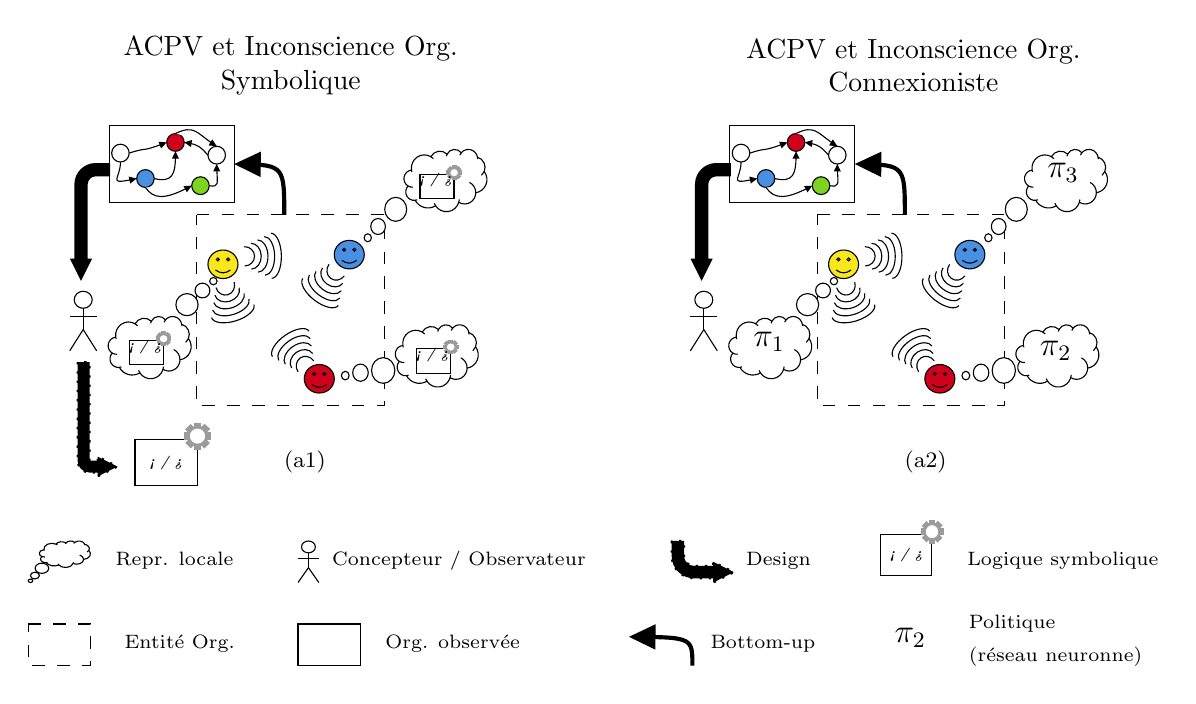
\begin{tikzpicture}[x=0.75pt,y=0.75pt,yscale=-1,xscale=1]
%uncomment if require: \path (0,1988); %set diagram left start at 0, and has height of 1988

%Shape: Rectangle [id:dp5013379967088911] 
\draw  [dash pattern={on 4.5pt off 4.5pt}] (91.18,1582.9) -- (181.55,1582.9) -- (181.55,1674.84) -- (91.18,1674.84) -- cycle ;
%Shape: Smiley Face [id:dp2909986828605782] 
\draw  [fill={rgb, 255:red, 248; green, 231; blue, 28 }  ,fill opacity=1 ] (96.6,1606.68) .. controls (96.6,1602.89) and (99.84,1599.82) .. (103.83,1599.82) .. controls (107.82,1599.82) and (111.06,1602.89) .. (111.06,1606.68) .. controls (111.06,1610.48) and (107.82,1613.55) .. (103.83,1613.55) .. controls (99.84,1613.55) and (96.6,1610.48) .. (96.6,1606.68) -- cycle ; \draw  [fill={rgb, 255:red, 248; green, 231; blue, 28 }  ,fill opacity=1 ] (100.65,1604.35) .. controls (100.65,1603.97) and (100.97,1603.66) .. (101.37,1603.66) .. controls (101.77,1603.66) and (102.09,1603.97) .. (102.09,1604.35) .. controls (102.09,1604.73) and (101.77,1605.04) .. (101.37,1605.04) .. controls (100.97,1605.04) and (100.65,1604.73) .. (100.65,1604.35) -- cycle ; \draw  [fill={rgb, 255:red, 248; green, 231; blue, 28 }  ,fill opacity=1 ] (105.56,1604.35) .. controls (105.56,1603.97) and (105.89,1603.66) .. (106.29,1603.66) .. controls (106.69,1603.66) and (107.01,1603.97) .. (107.01,1604.35) .. controls (107.01,1604.73) and (106.69,1605.04) .. (106.29,1605.04) .. controls (105.89,1605.04) and (105.56,1604.73) .. (105.56,1604.35) -- cycle ; \draw   (100.21,1609.43) .. controls (102.62,1611.26) and (105.03,1611.26) .. (107.44,1609.43) ;
%Shape: Arc [id:dp29848310914124687] 
\draw  [draw opacity=0] (118.78,1626.11) .. controls (118.78,1626.11) and (118.78,1626.11) .. (118.78,1626.11) .. controls (119.55,1628.72) and (115.59,1632.23) .. (109.94,1633.95) .. controls (104.28,1635.67) and (99.08,1634.94) .. (98.31,1632.33) -- (108.55,1629.22) -- cycle ; \draw   (118.78,1626.11) .. controls (118.78,1626.11) and (118.78,1626.11) .. (118.78,1626.11) .. controls (119.55,1628.72) and (115.59,1632.23) .. (109.94,1633.95) .. controls (104.28,1635.67) and (99.08,1634.94) .. (98.31,1632.33) ;  
%Shape: Arc [id:dp5990837957773074] 
\draw  [draw opacity=0] (116.39,1623.4) .. controls (117.16,1626.01) and (113.86,1629.32) .. (109.01,1630.8) .. controls (104.17,1632.27) and (99.62,1631.35) .. (98.85,1628.74) -- (107.62,1626.07) -- cycle ; \draw   (116.39,1623.4) .. controls (117.16,1626.01) and (113.86,1629.32) .. (109.01,1630.8) .. controls (104.17,1632.27) and (99.62,1631.35) .. (98.85,1628.74) ;  
%Shape: Arc [id:dp6042231692023955] 
\draw  [draw opacity=0] (114.01,1620.7) .. controls (114.01,1620.7) and (114.01,1620.7) .. (114.01,1620.7) .. controls (114.77,1623.31) and (112.12,1626.42) .. (108.08,1627.65) .. controls (104.05,1628.87) and (100.15,1627.75) .. (99.39,1625.14) -- (106.7,1622.92) -- cycle ; \draw   (114.01,1620.7) .. controls (114.01,1620.7) and (114.01,1620.7) .. (114.01,1620.7) .. controls (114.77,1623.31) and (112.12,1626.42) .. (108.08,1627.65) .. controls (104.05,1628.87) and (100.15,1627.75) .. (99.39,1625.14) ;  
%Shape: Arc [id:dp2913688932032118] 
\draw  [draw opacity=0] (111.62,1617.99) .. controls (111.62,1617.99) and (111.62,1617.99) .. (111.62,1617.99) .. controls (111.62,1617.99) and (111.62,1617.99) .. (111.62,1617.99) .. controls (112.39,1620.6) and (110.39,1623.51) .. (107.16,1624.49) .. controls (103.93,1625.48) and (100.69,1624.16) .. (99.92,1621.55) -- (105.77,1619.77) -- cycle ; \draw   (111.62,1617.99) .. controls (111.62,1617.99) and (111.62,1617.99) .. (111.62,1617.99) .. controls (111.62,1617.99) and (111.62,1617.99) .. (111.62,1617.99) .. controls (112.39,1620.6) and (110.39,1623.51) .. (107.16,1624.49) .. controls (103.93,1625.48) and (100.69,1624.16) .. (99.92,1621.55) ;  
%Shape: Arc [id:dp837702747005986] 
\draw  [draw opacity=0] (109.23,1615.28) .. controls (109.23,1615.28) and (109.23,1615.28) .. (109.23,1615.28) .. controls (110,1617.89) and (108.66,1620.61) .. (106.23,1621.34) .. controls (103.81,1622.08) and (101.23,1620.56) .. (100.46,1617.95) -- (104.84,1616.62) -- cycle ; \draw   (109.23,1615.28) .. controls (109.23,1615.28) and (109.23,1615.28) .. (109.23,1615.28) .. controls (110,1617.89) and (108.66,1620.61) .. (106.23,1621.34) .. controls (103.81,1622.08) and (101.23,1620.56) .. (100.46,1617.95) ;  

%Shape: Arc [id:dp942335351617398] 
\draw  [draw opacity=0] (126.91,1591.72) .. controls (126.91,1591.72) and (126.91,1591.72) .. (126.91,1591.72) .. controls (129.58,1591.67) and (131.85,1596.49) .. (131.96,1602.49) .. controls (132.08,1608.49) and (130,1613.4) .. (127.33,1613.45) -- (127.12,1602.59) -- cycle ; \draw   (126.91,1591.72) .. controls (126.91,1591.72) and (126.91,1591.72) .. (126.91,1591.72) .. controls (129.58,1591.67) and (131.85,1596.49) .. (131.96,1602.49) .. controls (132.08,1608.49) and (130,1613.4) .. (127.33,1613.45) ;  
%Shape: Arc [id:dp9374644640080091] 
\draw  [draw opacity=0] (123.7,1593.34) .. controls (126.38,1593.28) and (128.63,1597.41) .. (128.73,1602.55) .. controls (128.83,1607.7) and (126.74,1611.91) .. (124.07,1611.96) -- (123.88,1602.65) -- cycle ; \draw   (123.7,1593.34) .. controls (126.38,1593.28) and (128.63,1597.41) .. (128.73,1602.55) .. controls (128.83,1607.7) and (126.74,1611.91) .. (124.07,1611.96) ;  
%Shape: Arc [id:dp9875326017202676] 
\draw  [draw opacity=0] (120.5,1594.95) .. controls (120.5,1594.95) and (120.5,1594.95) .. (120.5,1594.95) .. controls (120.5,1594.95) and (120.5,1594.95) .. (120.5,1594.95) .. controls (123.18,1594.9) and (125.42,1598.33) .. (125.5,1602.62) .. controls (125.58,1606.9) and (123.48,1610.42) .. (120.8,1610.48) -- (120.65,1602.72) -- cycle ; \draw   (120.5,1594.95) .. controls (120.5,1594.95) and (120.5,1594.95) .. (120.5,1594.95) .. controls (120.5,1594.95) and (120.5,1594.95) .. (120.5,1594.95) .. controls (123.18,1594.9) and (125.42,1598.33) .. (125.5,1602.62) .. controls (125.58,1606.9) and (123.48,1610.42) .. (120.8,1610.48) ;  
%Shape: Arc [id:dp6395434963239012] 
\draw  [draw opacity=0] (117.3,1596.57) .. controls (119.98,1596.52) and (122.2,1599.25) .. (122.27,1602.68) .. controls (122.34,1606.11) and (120.22,1608.94) .. (117.54,1608.99) -- (117.42,1602.78) -- cycle ; \draw   (117.3,1596.57) .. controls (119.98,1596.52) and (122.2,1599.25) .. (122.27,1602.68) .. controls (122.34,1606.11) and (120.22,1608.94) .. (117.54,1608.99) ;  
%Shape: Arc [id:dp8898894473533424] 
\draw  [draw opacity=0] (114.1,1598.19) .. controls (114.1,1598.19) and (114.1,1598.19) .. (114.1,1598.19) .. controls (116.78,1598.13) and (118.99,1600.18) .. (119.04,1602.75) .. controls (119.09,1605.32) and (116.96,1607.45) .. (114.28,1607.5) -- (114.19,1602.85) -- cycle ; \draw   (114.1,1598.19) .. controls (114.1,1598.19) and (114.1,1598.19) .. (114.1,1598.19) .. controls (116.78,1598.13) and (118.99,1600.18) .. (119.04,1602.75) .. controls (119.09,1605.32) and (116.96,1607.45) .. (114.28,1607.5) ;  

%Shape: Smiley Face [id:dp7764061124552845] 
\draw  [fill={rgb, 255:red, 208; green, 2; blue, 27 }  ,fill opacity=1 ] (142.99,1661.85) .. controls (142.99,1658.05) and (146.22,1654.98) .. (150.22,1654.98) .. controls (154.21,1654.98) and (157.45,1658.05) .. (157.45,1661.85) .. controls (157.45,1665.64) and (154.21,1668.71) .. (150.22,1668.71) .. controls (146.22,1668.71) and (142.99,1665.64) .. (142.99,1661.85) -- cycle ; \draw  [fill={rgb, 255:red, 208; green, 2; blue, 27 }  ,fill opacity=1 ] (147.04,1659.51) .. controls (147.04,1659.13) and (147.36,1658.82) .. (147.76,1658.82) .. controls (148.16,1658.82) and (148.48,1659.13) .. (148.48,1659.51) .. controls (148.48,1659.89) and (148.16,1660.2) .. (147.76,1660.2) .. controls (147.36,1660.2) and (147.04,1659.89) .. (147.04,1659.51) -- cycle ; \draw  [fill={rgb, 255:red, 208; green, 2; blue, 27 }  ,fill opacity=1 ] (151.95,1659.51) .. controls (151.95,1659.13) and (152.28,1658.82) .. (152.68,1658.82) .. controls (153.07,1658.82) and (153.4,1659.13) .. (153.4,1659.51) .. controls (153.4,1659.89) and (153.07,1660.2) .. (152.68,1660.2) .. controls (152.28,1660.2) and (151.95,1659.89) .. (151.95,1659.51) -- cycle ; \draw   (146.6,1664.59) .. controls (149.01,1666.42) and (151.42,1666.42) .. (153.83,1664.59) ;
%Shape: Arc [id:dp6351137443890205] 
\draw  [draw opacity=0] (127.66,1651.18) .. controls (127.66,1651.18) and (127.66,1651.18) .. (127.66,1651.18) .. controls (126.14,1648.93) and (128.86,1644.36) .. (133.72,1640.96) .. controls (138.59,1637.57) and (143.76,1636.64) .. (145.28,1638.88) -- (136.47,1645.03) -- cycle ; \draw   (127.66,1651.18) .. controls (127.66,1651.18) and (127.66,1651.18) .. (127.66,1651.18) .. controls (126.14,1648.93) and (128.86,1644.36) .. (133.72,1640.96) .. controls (138.59,1637.57) and (143.76,1636.64) .. (145.28,1638.88) ;  
%Shape: Arc [id:dp14384542342253448] 
\draw  [draw opacity=0] (130.74,1653.01) .. controls (130.74,1653.01) and (130.74,1653.01) .. (130.74,1653.01) .. controls (129.23,1650.76) and (131.38,1646.58) .. (135.55,1643.67) .. controls (139.72,1640.76) and (144.33,1640.23) .. (145.85,1642.47) -- (138.29,1647.74) -- cycle ; \draw   (130.74,1653.01) .. controls (130.74,1653.01) and (130.74,1653.01) .. (130.74,1653.01) .. controls (129.23,1650.76) and (131.38,1646.58) .. (135.55,1643.67) .. controls (139.72,1640.76) and (144.33,1640.23) .. (145.85,1642.47) ;  
%Shape: Arc [id:dp5122941757438816] 
\draw  [draw opacity=0] (133.83,1654.84) .. controls (132.32,1652.6) and (133.91,1648.81) .. (137.38,1646.39) .. controls (140.86,1643.96) and (144.9,1643.82) .. (146.42,1646.06) -- (140.12,1650.45) -- cycle ; \draw   (133.83,1654.84) .. controls (132.32,1652.6) and (133.91,1648.81) .. (137.38,1646.39) .. controls (140.86,1643.96) and (144.9,1643.82) .. (146.42,1646.06) ;  
%Shape: Arc [id:dp07424291454569965] 
\draw  [draw opacity=0] (136.92,1656.68) .. controls (136.92,1656.68) and (136.92,1656.68) .. (136.92,1656.68) .. controls (135.4,1654.43) and (136.43,1651.04) .. (139.21,1649.1) .. controls (141.99,1647.16) and (145.47,1647.41) .. (146.99,1649.65) -- (141.95,1653.17) -- cycle ; \draw   (136.92,1656.68) .. controls (136.92,1656.68) and (136.92,1656.68) .. (136.92,1656.68) .. controls (135.4,1654.43) and (136.43,1651.04) .. (139.21,1649.1) .. controls (141.99,1647.16) and (145.47,1647.41) .. (146.99,1649.65) ;  
%Shape: Arc [id:dp21630199602073374] 
\draw  [draw opacity=0] (140,1658.51) .. controls (140,1658.51) and (140,1658.51) .. (140,1658.51) .. controls (138.49,1656.27) and (138.95,1653.26) .. (141.04,1651.81) .. controls (143.12,1650.36) and (146.04,1651) .. (147.55,1653.24) -- (143.78,1655.88) -- cycle ; \draw   (140,1658.51) .. controls (140,1658.51) and (140,1658.51) .. (140,1658.51) .. controls (138.49,1656.27) and (138.95,1653.26) .. (141.04,1651.81) .. controls (143.12,1650.36) and (146.04,1651) .. (147.55,1653.24) ;  

%Shape: Smiley Face [id:dp08426871234533728] 
\draw  [fill={rgb, 255:red, 74; green, 144; blue, 226 }  ,fill opacity=1 ] (157.45,1602.03) .. controls (157.45,1598.23) and (160.68,1595.16) .. (164.68,1595.16) .. controls (168.67,1595.16) and (171.91,1598.23) .. (171.91,1602.03) .. controls (171.91,1605.82) and (168.67,1608.89) .. (164.68,1608.89) .. controls (160.68,1608.89) and (157.45,1605.82) .. (157.45,1602.03) -- cycle ; \draw  [fill={rgb, 255:red, 74; green, 144; blue, 226 }  ,fill opacity=1 ] (161.5,1599.69) .. controls (161.5,1599.31) and (161.82,1599.01) .. (162.22,1599.01) .. controls (162.62,1599.01) and (162.94,1599.31) .. (162.94,1599.69) .. controls (162.94,1600.07) and (162.62,1600.38) .. (162.22,1600.38) .. controls (161.82,1600.38) and (161.5,1600.07) .. (161.5,1599.69) -- cycle ; \draw  [fill={rgb, 255:red, 74; green, 144; blue, 226 }  ,fill opacity=1 ] (166.41,1599.69) .. controls (166.41,1599.31) and (166.74,1599.01) .. (167.13,1599.01) .. controls (167.53,1599.01) and (167.86,1599.31) .. (167.86,1599.69) .. controls (167.86,1600.07) and (167.53,1600.38) .. (167.13,1600.38) .. controls (166.74,1600.38) and (166.41,1600.07) .. (166.41,1599.69) -- cycle ; \draw   (161.06,1604.77) .. controls (163.47,1606.6) and (165.88,1606.6) .. (168.29,1604.77) ;
%Shape: Arc [id:dp02754459389784214] 
\draw  [draw opacity=0] (159.38,1626.55) .. controls (159.38,1626.55) and (159.38,1626.55) .. (159.38,1626.55) .. controls (157.77,1628.72) and (152.64,1627.57) .. (147.92,1623.98) .. controls (143.2,1620.38) and (140.68,1615.69) .. (142.28,1613.51) -- (150.83,1620.03) -- cycle ; \draw   (159.38,1626.55) .. controls (159.38,1626.55) and (159.38,1626.55) .. (159.38,1626.55) .. controls (157.77,1628.72) and (152.64,1627.57) .. (147.92,1623.98) .. controls (143.2,1620.38) and (140.68,1615.69) .. (142.28,1613.51) ;  
%Shape: Arc [id:dp8443099266344009] 
\draw  [draw opacity=0] (160.1,1622.98) .. controls (160.1,1622.98) and (160.1,1622.98) .. (160.1,1622.98) .. controls (160.1,1622.98) and (160.1,1622.98) .. (160.1,1622.98) .. controls (158.49,1625.16) and (153.91,1624.43) .. (149.86,1621.34) .. controls (145.81,1618.26) and (143.84,1613.99) .. (145.44,1611.81) -- (152.77,1617.4) -- cycle ; \draw   (160.1,1622.98) .. controls (160.1,1622.98) and (160.1,1622.98) .. (160.1,1622.98) .. controls (160.1,1622.98) and (160.1,1622.98) .. (160.1,1622.98) .. controls (158.49,1625.16) and (153.91,1624.43) .. (149.86,1621.34) .. controls (145.81,1618.26) and (143.84,1613.99) .. (145.44,1611.81) ;  
%Shape: Arc [id:dp36090403949084215] 
\draw  [draw opacity=0] (160.81,1619.42) .. controls (159.21,1621.6) and (155.17,1621.28) .. (151.8,1618.71) .. controls (148.43,1616.14) and (146.99,1612.29) .. (148.6,1610.11) -- (154.71,1614.77) -- cycle ; \draw   (160.81,1619.42) .. controls (159.21,1621.6) and (155.17,1621.28) .. (151.8,1618.71) .. controls (148.43,1616.14) and (146.99,1612.29) .. (148.6,1610.11) ;  
%Shape: Arc [id:dp8389598515474829] 
\draw  [draw opacity=0] (161.53,1615.86) .. controls (161.53,1615.86) and (161.53,1615.86) .. (161.53,1615.86) .. controls (159.92,1618.04) and (156.44,1618.14) .. (153.74,1616.08) .. controls (151.04,1614.02) and (150.15,1610.59) .. (151.76,1608.41) -- (156.65,1612.13) -- cycle ; \draw   (161.53,1615.86) .. controls (161.53,1615.86) and (161.53,1615.86) .. (161.53,1615.86) .. controls (159.92,1618.04) and (156.44,1618.14) .. (153.74,1616.08) .. controls (151.04,1614.02) and (150.15,1610.59) .. (151.76,1608.41) ;  
%Shape: Arc [id:dp45749711978150187] 
\draw  [draw opacity=0] (162.25,1612.29) .. controls (162.25,1612.29) and (162.25,1612.29) .. (162.25,1612.29) .. controls (162.25,1612.29) and (162.25,1612.29) .. (162.25,1612.29) .. controls (160.64,1614.47) and (157.7,1614.99) .. (155.68,1613.45) .. controls (153.65,1611.91) and (153.31,1608.89) .. (154.92,1606.71) -- (158.58,1609.5) -- cycle ; \draw   (162.25,1612.29) .. controls (162.25,1612.29) and (162.25,1612.29) .. (162.25,1612.29) .. controls (162.25,1612.29) and (162.25,1612.29) .. (162.25,1612.29) .. controls (160.64,1614.47) and (157.7,1614.99) .. (155.68,1613.45) .. controls (153.65,1611.91) and (153.31,1608.89) .. (154.92,1606.71) ;  

%Shape: Rectangle [id:dp7060287107715945] 
\draw  [fill={rgb, 255:red, 255; green, 255; blue, 255 }  ,fill opacity=1 ] (49,1540) -- (109.25,1540) -- (109.25,1576.77) -- (49,1576.77) -- cycle ;
%Shape: Ellipse [id:dp8204500766763589] 
\draw  [fill={rgb, 255:red, 255; green, 255; blue, 255 }  ,fill opacity=1 ] (50.21,1553.12) .. controls (50.21,1550.75) and (52.1,1548.83) .. (54.43,1548.83) .. controls (56.76,1548.83) and (58.64,1550.75) .. (58.64,1553.12) .. controls (58.64,1555.49) and (56.76,1557.41) .. (54.43,1557.41) .. controls (52.1,1557.41) and (50.21,1555.49) .. (50.21,1553.12) -- cycle ;
%Shape: Ellipse [id:dp5181525806308303] 
\draw  [fill={rgb, 255:red, 74; green, 144; blue, 226 }  ,fill opacity=1 ] (62.26,1565.37) .. controls (62.26,1563) and (64.15,1561.08) .. (66.48,1561.08) .. controls (68.81,1561.08) and (70.69,1563) .. (70.69,1565.37) .. controls (70.69,1567.74) and (68.81,1569.66) .. (66.48,1569.66) .. controls (64.15,1569.66) and (62.26,1567.74) .. (62.26,1565.37) -- cycle ;
%Shape: Ellipse [id:dp0906893320423029] 
\draw  [fill={rgb, 255:red, 208; green, 2; blue, 27 }  ,fill opacity=1 ] (76.72,1547.97) .. controls (76.72,1545.6) and (78.61,1543.68) .. (80.94,1543.68) .. controls (83.26,1543.68) and (85.15,1545.6) .. (85.15,1547.97) .. controls (85.15,1550.34) and (83.26,1552.26) .. (80.94,1552.26) .. controls (78.61,1552.26) and (76.72,1550.34) .. (76.72,1547.97) -- cycle ;
%Shape: Ellipse [id:dp3404459677220828] 
\draw  [fill={rgb, 255:red, 255; green, 255; blue, 255 }  ,fill opacity=1 ] (96.6,1554.1) .. controls (96.6,1551.73) and (98.49,1549.81) .. (100.82,1549.81) .. controls (103.15,1549.81) and (105.03,1551.73) .. (105.03,1554.1) .. controls (105.03,1556.47) and (103.15,1558.39) .. (100.82,1558.39) .. controls (98.49,1558.39) and (96.6,1556.47) .. (96.6,1554.1) -- cycle ;
%Shape: Ellipse [id:dp7841877382320065] 
\draw  [fill={rgb, 255:red, 126; green, 211; blue, 33 }  ,fill opacity=1 ] (88.77,1568.81) .. controls (88.77,1566.44) and (90.66,1564.52) .. (92.98,1564.52) .. controls (95.31,1564.52) and (97.2,1566.44) .. (97.2,1568.81) .. controls (97.2,1571.18) and (95.31,1573.1) .. (92.98,1573.1) .. controls (90.66,1573.1) and (88.77,1571.18) .. (88.77,1568.81) -- cycle ;
%Curve Lines [id:da8931114055545611] 
\draw [fill={rgb, 255:red, 255; green, 255; blue, 255 }  ,fill opacity=1 ]   (58.64,1553.12) .. controls (68.12,1550.05) and (63.67,1552.76) .. (73.92,1549.01) ;
\draw [shift={(76.72,1547.97)}, rotate = 159.17] [fill={rgb, 255:red, 0; green, 0; blue, 0 }  ][line width=0.08]  [draw opacity=0] (3.57,-1.72) -- (0,0) -- (3.57,1.72) -- cycle    ;
%Curve Lines [id:da7735282082131947] 
\draw [fill={rgb, 255:red, 255; green, 255; blue, 255 }  ,fill opacity=1 ]   (70.69,1565.37) .. controls (79.76,1567.65) and (80.8,1562.63) .. (80.92,1555.25) ;
\draw [shift={(80.94,1552.26)}, rotate = 90] [fill={rgb, 255:red, 0; green, 0; blue, 0 }  ][line width=0.08]  [draw opacity=0] (3.57,-1.72) -- (0,0) -- (3.57,1.72) -- cycle    ;
%Curve Lines [id:da8607237334353054] 
\draw [fill={rgb, 255:red, 255; green, 255; blue, 255 }  ,fill opacity=1 ]   (96.6,1554.1) .. controls (93.1,1550.33) and (92.09,1549.27) .. (88.06,1548.46) ;
\draw [shift={(85.15,1547.97)}, rotate = 8.42] [fill={rgb, 255:red, 0; green, 0; blue, 0 }  ][line width=0.08]  [draw opacity=0] (3.57,-1.72) -- (0,0) -- (3.57,1.72) -- cycle    ;
%Curve Lines [id:da39004498418287703] 
\draw [fill={rgb, 255:red, 255; green, 255; blue, 255 }  ,fill opacity=1 ]   (97.2,1568.81) .. controls (101.97,1569.67) and (101.15,1567.87) .. (100.88,1561.33) ;
\draw [shift={(100.82,1558.39)}, rotate = 90] [fill={rgb, 255:red, 0; green, 0; blue, 0 }  ][line width=0.08]  [draw opacity=0] (3.57,-1.72) -- (0,0) -- (3.57,1.72) -- cycle    ;
%Curve Lines [id:da9723906849673678] 
\draw [fill={rgb, 255:red, 255; green, 255; blue, 255 }  ,fill opacity=1 ]   (54.43,1557.41) .. controls (54.43,1565.5) and (48.17,1568.19) .. (59.41,1565.96) ;
\draw [shift={(62.26,1565.37)}, rotate = 168.05] [fill={rgb, 255:red, 0; green, 0; blue, 0 }  ][line width=0.08]  [draw opacity=0] (3.57,-1.72) -- (0,0) -- (3.57,1.72) -- cycle    ;
%Curve Lines [id:da2389978943863197] 
\draw [fill={rgb, 255:red, 255; green, 255; blue, 255 }  ,fill opacity=1 ]   (66.48,1569.66) .. controls (70.38,1575.45) and (75.82,1575.36) .. (86.16,1570.17) ;
\draw [shift={(88.77,1568.81)}, rotate = 151.67] [fill={rgb, 255:red, 0; green, 0; blue, 0 }  ][line width=0.08]  [draw opacity=0] (3.57,-1.72) -- (0,0) -- (3.57,1.72) -- cycle    ;
%Curve Lines [id:da9606608376740503] 
\draw [fill={rgb, 255:red, 255; green, 255; blue, 255 }  ,fill opacity=1 ]   (80.94,1543.68) .. controls (89.71,1539.44) and (91,1543.12) .. (98.42,1548.25) ;
\draw [shift={(100.82,1549.81)}, rotate = 211.4] [fill={rgb, 255:red, 0; green, 0; blue, 0 }  ][line width=0.08]  [draw opacity=0] (3.57,-1.72) -- (0,0) -- (3.57,1.72) -- cycle    ;
%Shape: Ellipse [id:dp8238624688148318] 
\draw   (32.16,1623.78) .. controls (32.16,1621.51) and (34.1,1619.68) .. (36.49,1619.68) .. controls (38.88,1619.68) and (40.82,1621.51) .. (40.82,1623.78) .. controls (40.82,1626.04) and (38.88,1627.88) .. (36.49,1627.88) .. controls (34.1,1627.88) and (32.16,1626.04) .. (32.16,1623.78) -- cycle ;
%Straight Lines [id:da1506125445454658] 
\draw    (36.49,1627.88) -- (36.49,1638.12) ;
%Straight Lines [id:da49468464160952785] 
\draw    (36.49,1638.12) -- (30,1648.37) ;
%Straight Lines [id:da131299671574843] 
\draw    (36.49,1638.12) -- (42.98,1648.37) ;
%Straight Lines [id:da7804526802882297] 
\draw    (42.98,1631.98) -- (30,1631.98) ;

%Bend Arrow [id:dp6575031643828187] 
\draw  [fill={rgb, 255:red, 0; green, 0; blue, 0 }  ,fill opacity=1 ][line width=0.75]  (49,1558.39) -- (42.5,1558.39) .. controls (37.11,1558.39) and (32.74,1562.76) .. (32.74,1568.15) -- (32.74,1604.51) -- (30.93,1604.51) -- (35.45,1613.55) -- (39.97,1604.51) -- (38.16,1604.51) -- (38.16,1568.15) .. controls (38.16,1565.75) and (40.1,1563.81) .. (42.5,1563.81) -- (49,1563.81) -- cycle ;
%Shape: Boxed Bezier Curve [id:dp6472304808727206] 
\draw [line width=1.5]    (133.35,1582.9) .. controls (133.35,1559.97) and (133.35,1558.71) .. (113.01,1558.43) ;
\draw [shift={(109.25,1558.39)}, rotate = 0.58] [fill={rgb, 255:red, 0; green, 0; blue, 0 }  ][line width=0.08]  [draw opacity=0] (12.77,-6.13) -- (0,0) -- (12.77,6.13) -- cycle    ;

%Shape: Cloud [id:dp9267969156542857] 
\draw  [fill={rgb, 255:red, 255; green, 255; blue, 255 }  ,fill opacity=1 ] (52.14,1641.72) .. controls (51.82,1639.3) and (52.88,1636.9) .. (54.86,1635.55) .. controls (56.85,1634.19) and (59.42,1634.12) .. (61.48,1635.35) .. controls (62.21,1633.95) and (63.55,1632.97) .. (65.09,1632.73) .. controls (66.63,1632.49) and (68.19,1633.01) .. (69.3,1634.12) .. controls (69.92,1632.85) and (71.14,1631.99) .. (72.53,1631.86) .. controls (73.92,1631.72) and (75.28,1632.33) .. (76.12,1633.46) .. controls (77.24,1632.11) and (79.03,1631.54) .. (80.71,1632) .. controls (82.39,1632.46) and (83.66,1633.87) .. (83.97,1635.61) .. controls (85.34,1636) and (86.49,1636.97) .. (87.11,1638.29) .. controls (87.73,1639.6) and (87.77,1641.13) .. (87.2,1642.47) .. controls (88.56,1644.28) and (88.88,1646.68) .. (88.04,1648.79) .. controls (87.2,1650.89) and (85.33,1652.38) .. (83.12,1652.71) .. controls (83.11,1654.68) and (82.05,1656.5) .. (80.35,1657.45) .. controls (78.65,1658.4) and (76.58,1658.34) .. (74.94,1657.3) .. controls (74.24,1659.66) and (72.27,1661.41) .. (69.88,1661.77) .. controls (67.49,1662.13) and (65.12,1661.05) .. (63.77,1659) .. controls (62.13,1660.01) and (60.15,1660.3) .. (58.3,1659.81) .. controls (56.44,1659.31) and (54.86,1658.07) .. (53.9,1656.36) .. controls (52.22,1656.56) and (50.6,1655.67) .. (49.83,1654.13) .. controls (49.07,1652.6) and (49.33,1650.73) .. (50.49,1649.48) .. controls (48.99,1648.57) and (48.22,1646.78) .. (48.59,1645.04) .. controls (48.96,1643.3) and (50.38,1641.99) .. (52.11,1641.81) ; \draw   (50.49,1649.48) .. controls (51.2,1649.9) and (52.01,1650.09) .. (52.83,1650.03)(53.9,1656.36) .. controls (54.25,1656.32) and (54.6,1656.23) .. (54.93,1656.1)(63.77,1659) .. controls (63.53,1658.62) and (63.32,1658.21) .. (63.16,1657.79)(74.94,1657.3) .. controls (75.07,1656.86) and (75.15,1656.42) .. (75.19,1655.97)(83.12,1652.71) .. controls (83.14,1650.6) and (81.97,1648.68) .. (80.11,1647.75)(87.2,1642.47) .. controls (86.9,1643.19) and (86.44,1643.82) .. (85.86,1644.33)(83.97,1635.61) .. controls (84.02,1635.9) and (84.04,1636.19) .. (84.04,1636.49)(76.12,1633.46) .. controls (75.84,1633.8) and (75.61,1634.18) .. (75.43,1634.58)(69.3,1634.12) .. controls (69.15,1634.43) and (69.04,1634.75) .. (68.97,1635.09)(61.48,1635.35) .. controls (61.92,1635.61) and (62.32,1635.93) .. (62.69,1636.29)(52.14,1641.72) .. controls (52.18,1642.05) and (52.25,1642.38) .. (52.35,1642.7) ;
%Shape: Cloud [id:dp5528798724302991] 
\draw  [fill={rgb, 255:red, 255; green, 255; blue, 255 }  ,fill opacity=1 ] (194.64,1561.22) .. controls (194.32,1558.8) and (195.38,1556.4) .. (197.36,1555.05) .. controls (199.35,1553.69) and (201.92,1553.62) .. (203.98,1554.85) .. controls (204.71,1553.45) and (206.05,1552.47) .. (207.59,1552.23) .. controls (209.13,1551.99) and (210.69,1552.51) .. (211.8,1553.62) .. controls (212.42,1552.35) and (213.64,1551.49) .. (215.03,1551.36) .. controls (216.42,1551.22) and (217.78,1551.83) .. (218.62,1552.96) .. controls (219.74,1551.61) and (221.53,1551.04) .. (223.21,1551.5) .. controls (224.89,1551.96) and (226.16,1553.37) .. (226.47,1555.11) .. controls (227.84,1555.5) and (228.99,1556.47) .. (229.61,1557.79) .. controls (230.23,1559.1) and (230.27,1560.63) .. (229.7,1561.97) .. controls (231.06,1563.78) and (231.38,1566.18) .. (230.54,1568.29) .. controls (229.7,1570.39) and (227.83,1571.88) .. (225.62,1572.21) .. controls (225.61,1574.18) and (224.55,1576) .. (222.85,1576.95) .. controls (221.15,1577.9) and (219.08,1577.84) .. (217.44,1576.8) .. controls (216.74,1579.16) and (214.77,1580.91) .. (212.38,1581.27) .. controls (209.99,1581.63) and (207.62,1580.55) .. (206.27,1578.5) .. controls (204.63,1579.51) and (202.65,1579.8) .. (200.8,1579.31) .. controls (198.94,1578.81) and (197.36,1577.57) .. (196.4,1575.86) .. controls (194.72,1576.06) and (193.1,1575.17) .. (192.33,1573.63) .. controls (191.57,1572.1) and (191.83,1570.23) .. (192.99,1568.98) .. controls (191.49,1568.07) and (190.72,1566.28) .. (191.09,1564.54) .. controls (191.46,1562.8) and (192.88,1561.49) .. (194.61,1561.31) ; \draw   (192.99,1568.98) .. controls (193.7,1569.4) and (194.51,1569.59) .. (195.33,1569.53)(196.4,1575.86) .. controls (196.75,1575.82) and (197.1,1575.73) .. (197.43,1575.6)(206.27,1578.5) .. controls (206.03,1578.12) and (205.82,1577.71) .. (205.66,1577.29)(217.44,1576.8) .. controls (217.57,1576.36) and (217.65,1575.92) .. (217.69,1575.47)(225.62,1572.21) .. controls (225.64,1570.1) and (224.47,1568.18) .. (222.61,1567.25)(229.7,1561.97) .. controls (229.4,1562.69) and (228.94,1563.32) .. (228.36,1563.83)(226.47,1555.11) .. controls (226.52,1555.4) and (226.54,1555.69) .. (226.54,1555.99)(218.62,1552.96) .. controls (218.34,1553.3) and (218.11,1553.68) .. (217.93,1554.08)(211.8,1553.62) .. controls (211.65,1553.93) and (211.54,1554.25) .. (211.47,1554.59)(203.98,1554.85) .. controls (204.42,1555.11) and (204.82,1555.43) .. (205.19,1555.79)(194.64,1561.22) .. controls (194.68,1561.55) and (194.75,1561.88) .. (194.85,1562.2) ;
%Shape: Ellipse [id:dp7514204534640926] 
\draw  [fill={rgb, 255:red, 255; green, 255; blue, 255 }  ,fill opacity=1 ] (175.03,1588.48) .. controls (175.03,1586.36) and (176.61,1584.63) .. (178.56,1584.63) .. controls (180.51,1584.63) and (182.09,1586.36) .. (182.09,1588.48) .. controls (182.09,1590.6) and (180.51,1592.33) .. (178.56,1592.33) .. controls (176.61,1592.33) and (175.03,1590.6) .. (175.03,1588.48) -- cycle ;
%Shape: Ellipse [id:dp44553318612962955] 
\draw  [fill={rgb, 255:red, 255; green, 255; blue, 255 }  ,fill opacity=1 ] (171.83,1593.92) .. controls (171.83,1592.85) and (172.62,1591.99) .. (173.6,1591.99) .. controls (174.57,1591.99) and (175.36,1592.85) .. (175.36,1593.92) .. controls (175.36,1594.98) and (174.57,1595.84) .. (173.6,1595.84) .. controls (172.62,1595.84) and (171.83,1594.98) .. (171.83,1593.92) -- cycle ;
%Shape: Ellipse [id:dp82913236602551] 
\draw  [fill={rgb, 255:red, 255; green, 255; blue, 255 }  ,fill opacity=1 ] (90.37,1619.32) .. controls (90.37,1617.36) and (91.97,1615.77) .. (93.94,1615.77) .. controls (95.91,1615.77) and (97.51,1617.36) .. (97.51,1619.32) .. controls (97.51,1621.28) and (95.91,1622.87) .. (93.94,1622.87) .. controls (91.97,1622.87) and (90.37,1621.28) .. (90.37,1619.32) -- cycle ;
%Shape: Ellipse [id:dp2375828747719494] 
\draw  [fill={rgb, 255:red, 255; green, 255; blue, 255 }  ,fill opacity=1 ] (81.14,1626.14) .. controls (81.14,1623.2) and (83.53,1620.81) .. (86.49,1620.81) .. controls (89.44,1620.81) and (91.84,1623.2) .. (91.84,1626.14) .. controls (91.84,1629.08) and (89.44,1631.46) .. (86.49,1631.46) .. controls (83.53,1631.46) and (81.14,1629.08) .. (81.14,1626.14) -- cycle ;
%Shape: Ellipse [id:dp42236739615338126] 
\draw  [fill={rgb, 255:red, 255; green, 255; blue, 255 }  ,fill opacity=1 ] (97.42,1614.8) .. controls (97.42,1613.82) and (98.22,1613.02) .. (99.2,1613.02) .. controls (100.19,1613.02) and (100.98,1613.82) .. (100.98,1614.8) .. controls (100.98,1615.78) and (100.19,1616.57) .. (99.2,1616.57) .. controls (98.22,1616.57) and (97.42,1615.78) .. (97.42,1614.8) -- cycle ;
%Shape: Ellipse [id:dp9447534834781316] 
\draw  [fill={rgb, 255:red, 255; green, 255; blue, 255 }  ,fill opacity=1 ] (181.75,1580.2) .. controls (181.75,1577.01) and (184.13,1574.43) .. (187.05,1574.43) .. controls (189.97,1574.43) and (192.34,1577.01) .. (192.34,1580.2) .. controls (192.34,1583.38) and (189.97,1585.97) .. (187.05,1585.97) .. controls (184.13,1585.97) and (181.75,1583.38) .. (181.75,1580.2) -- cycle ;
%Shape: Ellipse [id:dp5194641468129697] 
\draw  [fill={rgb, 255:red, 255; green, 255; blue, 255 }  ,fill opacity=1 ] (175.41,1657.84) .. controls (175.41,1654.42) and (177.93,1651.65) .. (181.03,1651.65) .. controls (184.12,1651.65) and (186.64,1654.42) .. (186.64,1657.84) .. controls (186.64,1661.26) and (184.12,1664.03) .. (181.03,1664.03) .. controls (177.93,1664.03) and (175.41,1661.26) .. (175.41,1657.84) -- cycle ;
%Shape: Ellipse [id:dp7757831456715724] 
\draw  [fill={rgb, 255:red, 255; green, 255; blue, 255 }  ,fill opacity=1 ] (166.34,1658.91) .. controls (166.34,1656.63) and (168.02,1654.78) .. (170.08,1654.78) .. controls (172.15,1654.78) and (173.82,1656.63) .. (173.82,1658.91) .. controls (173.82,1661.19) and (172.15,1663.04) .. (170.08,1663.04) .. controls (168.02,1663.04) and (166.34,1661.19) .. (166.34,1658.91) -- cycle ;
%Shape: Ellipse [id:dp29373407797568707] 
\draw  [fill={rgb, 255:red, 255; green, 255; blue, 255 }  ,fill opacity=1 ] (160.88,1660.31) .. controls (160.88,1659.17) and (161.72,1658.25) .. (162.75,1658.25) .. controls (163.78,1658.25) and (164.62,1659.17) .. (164.62,1660.31) .. controls (164.62,1661.45) and (163.78,1662.38) .. (162.75,1662.38) .. controls (161.72,1662.38) and (160.88,1661.45) .. (160.88,1660.31) -- cycle ;
%Flowchart: Process [id:dp9834032610152076] 
\draw   (58.74,1643.45) -- (75.11,1643.45) -- (75.11,1655.13) -- (58.74,1655.13) -- cycle ;
%Shape: Ellipse [id:dp6640670880210211] 
\draw  [color={rgb, 255:red, 155; green, 155; blue, 155 }  ,draw opacity=1 ][fill={rgb, 255:red, 155; green, 155; blue, 155 }  ,fill opacity=1 ] (72.58,1642.54) .. controls (72.58,1641.17) and (73.76,1640.07) .. (75.22,1640.07) .. controls (76.68,1640.07) and (77.86,1641.17) .. (77.86,1642.54) .. controls (77.86,1643.91) and (76.68,1645.01) .. (75.22,1645.01) .. controls (73.76,1645.01) and (72.58,1643.91) .. (72.58,1642.54) -- cycle ;
%Shape: Rectangle [id:dp5232643763802065] 
\draw  [color={rgb, 255:red, 155; green, 155; blue, 155 }  ,draw opacity=1 ][fill={rgb, 255:red, 155; green, 155; blue, 155 }  ,fill opacity=1 ] (74.34,1639.24) -- (76.1,1639.24) -- (76.1,1640.89) -- (74.34,1640.89) -- cycle ;
%Shape: Rectangle [id:dp9098850223722781] 
\draw  [color={rgb, 255:red, 155; green, 155; blue, 155 }  ,draw opacity=1 ][fill={rgb, 255:red, 155; green, 155; blue, 155 }  ,fill opacity=1 ] (76.98,1641.72) -- (78.74,1641.72) -- (78.74,1643.36) -- (76.98,1643.36) -- cycle ;
%Shape: Rectangle [id:dp27460898986906623] 
\draw  [color={rgb, 255:red, 155; green, 155; blue, 155 }  ,draw opacity=1 ][fill={rgb, 255:red, 155; green, 155; blue, 155 }  ,fill opacity=1 ] (74.34,1644.19) -- (76.1,1644.19) -- (76.1,1645.84) -- (74.34,1645.84) -- cycle ;
%Shape: Rectangle [id:dp42946228539873565] 
\draw  [color={rgb, 255:red, 155; green, 155; blue, 155 }  ,draw opacity=1 ][fill={rgb, 255:red, 155; green, 155; blue, 155 }  ,fill opacity=1 ] (71.7,1641.72) -- (73.46,1641.72) -- (73.46,1643.36) -- (71.7,1643.36) -- cycle ;
%Shape: Rectangle [id:dp7904848912164214] 
\draw  [color={rgb, 255:red, 155; green, 155; blue, 155 }  ,draw opacity=1 ][fill={rgb, 255:red, 155; green, 155; blue, 155 }  ,fill opacity=1 ] (73.42,1639.69) -- (74.66,1640.86) -- (73.42,1642.02) -- (72.17,1640.86) -- cycle ;
%Shape: Rectangle [id:dp3301141202355372] 
\draw  [color={rgb, 255:red, 155; green, 155; blue, 155 }  ,draw opacity=1 ][fill={rgb, 255:red, 155; green, 155; blue, 155 }  ,fill opacity=1 ] (77.04,1643.12) -- (78.28,1644.29) -- (77.04,1645.45) -- (75.8,1644.29) -- cycle ;
%Shape: Rectangle [id:dp6342375560239414] 
\draw  [color={rgb, 255:red, 155; green, 155; blue, 155 }  ,draw opacity=1 ][fill={rgb, 255:red, 155; green, 155; blue, 155 }  ,fill opacity=1 ] (73.45,1643.09) -- (74.69,1644.26) -- (73.45,1645.42) -- (72.21,1644.26) -- cycle ;
%Shape: Rectangle [id:dp3754059778400457] 
\draw  [color={rgb, 255:red, 155; green, 155; blue, 155 }  ,draw opacity=1 ][fill={rgb, 255:red, 155; green, 155; blue, 155 }  ,fill opacity=1 ] (77.1,1639.59) -- (78.34,1640.76) -- (77.1,1641.93) -- (75.86,1640.76) -- cycle ;
%Shape: Ellipse [id:dp7736710329933231] 
\draw  [color={rgb, 255:red, 155; green, 155; blue, 155 }  ,draw opacity=1 ][fill={rgb, 255:red, 255; green, 255; blue, 255 }  ,fill opacity=1 ] (73.02,1642.54) .. controls (73.02,1641.4) and (74.01,1640.48) .. (75.22,1640.48) .. controls (76.44,1640.48) and (77.42,1641.4) .. (77.42,1642.54) .. controls (77.42,1643.68) and (76.44,1644.6) .. (75.22,1644.6) .. controls (74.01,1644.6) and (73.02,1643.68) .. (73.02,1642.54) -- cycle ;

%Shape: Cloud [id:dp8515242927252613] 
\draw  [fill={rgb, 255:red, 255; green, 255; blue, 255 }  ,fill opacity=1 ] (190.48,1645.72) .. controls (190.15,1643.3) and (191.21,1640.9) .. (193.2,1639.55) .. controls (195.19,1638.19) and (197.76,1638.12) .. (199.82,1639.35) .. controls (200.55,1637.95) and (201.89,1636.97) .. (203.43,1636.73) .. controls (204.97,1636.49) and (206.53,1637.01) .. (207.64,1638.12) .. controls (208.26,1636.85) and (209.48,1635.99) .. (210.87,1635.86) .. controls (212.25,1635.72) and (213.61,1636.33) .. (214.46,1637.46) .. controls (215.58,1636.11) and (217.37,1635.54) .. (219.05,1636) .. controls (220.73,1636.46) and (221.99,1637.87) .. (222.3,1639.61) .. controls (223.68,1640) and (224.83,1640.97) .. (225.45,1642.29) .. controls (226.07,1643.6) and (226.1,1645.13) .. (225.54,1646.47) .. controls (226.9,1648.28) and (227.21,1650.68) .. (226.37,1652.79) .. controls (225.53,1654.89) and (223.66,1656.38) .. (221.46,1656.71) .. controls (221.44,1658.68) and (220.38,1660.5) .. (218.68,1661.45) .. controls (216.99,1662.4) and (214.92,1662.34) .. (213.28,1661.3) .. controls (212.58,1663.66) and (210.61,1665.41) .. (208.22,1665.77) .. controls (205.83,1666.13) and (203.45,1665.05) .. (202.11,1663) .. controls (200.46,1664.01) and (198.49,1664.3) .. (196.63,1663.81) .. controls (194.78,1663.31) and (193.19,1662.07) .. (192.24,1660.36) .. controls (190.56,1660.56) and (188.93,1659.67) .. (188.17,1658.13) .. controls (187.41,1656.6) and (187.67,1654.73) .. (188.82,1653.48) .. controls (187.32,1652.57) and (186.56,1650.78) .. (186.93,1649.04) .. controls (187.3,1647.3) and (188.71,1645.99) .. (190.44,1645.81) ; \draw   (188.82,1653.48) .. controls (189.53,1653.9) and (190.35,1654.09) .. (191.17,1654.03)(192.24,1660.36) .. controls (192.59,1660.32) and (192.93,1660.23) .. (193.26,1660.1)(202.11,1663) .. controls (201.86,1662.62) and (201.65,1662.21) .. (201.49,1661.79)(213.28,1661.3) .. controls (213.4,1660.86) and (213.49,1660.42) .. (213.52,1659.97)(221.46,1656.71) .. controls (221.47,1654.6) and (220.3,1652.68) .. (218.45,1651.75)(225.54,1646.47) .. controls (225.24,1647.19) and (224.78,1647.82) .. (224.2,1648.33)(222.3,1639.61) .. controls (222.35,1639.9) and (222.38,1640.19) .. (222.37,1640.49)(214.46,1637.46) .. controls (214.18,1637.8) and (213.95,1638.18) .. (213.77,1638.58)(207.64,1638.12) .. controls (207.49,1638.43) and (207.37,1638.75) .. (207.3,1639.09)(199.82,1639.35) .. controls (200.26,1639.61) and (200.66,1639.93) .. (201.02,1640.29)(190.48,1645.72) .. controls (190.52,1646.05) and (190.59,1646.38) .. (190.69,1646.7) ;
%Flowchart: Process [id:dp26170799496979835] 
\draw   (197.08,1647.45) -- (213.44,1647.45) -- (213.44,1659.13) -- (197.08,1659.13) -- cycle ;
%Shape: Ellipse [id:dp7150327388817976] 
\draw  [color={rgb, 255:red, 155; green, 155; blue, 155 }  ,draw opacity=1 ][fill={rgb, 255:red, 155; green, 155; blue, 155 }  ,fill opacity=1 ] (210.92,1646.54) .. controls (210.92,1645.17) and (212.1,1644.07) .. (213.56,1644.07) .. controls (215.02,1644.07) and (216.2,1645.17) .. (216.2,1646.54) .. controls (216.2,1647.91) and (215.02,1649.01) .. (213.56,1649.01) .. controls (212.1,1649.01) and (210.92,1647.91) .. (210.92,1646.54) -- cycle ;
%Shape: Rectangle [id:dp23804105610818582] 
\draw  [color={rgb, 255:red, 155; green, 155; blue, 155 }  ,draw opacity=1 ][fill={rgb, 255:red, 155; green, 155; blue, 155 }  ,fill opacity=1 ] (212.68,1643.24) -- (214.44,1643.24) -- (214.44,1644.89) -- (212.68,1644.89) -- cycle ;
%Shape: Rectangle [id:dp19367155172233208] 
\draw  [color={rgb, 255:red, 155; green, 155; blue, 155 }  ,draw opacity=1 ][fill={rgb, 255:red, 155; green, 155; blue, 155 }  ,fill opacity=1 ] (215.32,1645.72) -- (217.08,1645.72) -- (217.08,1647.36) -- (215.32,1647.36) -- cycle ;
%Shape: Rectangle [id:dp9574367965081055] 
\draw  [color={rgb, 255:red, 155; green, 155; blue, 155 }  ,draw opacity=1 ][fill={rgb, 255:red, 155; green, 155; blue, 155 }  ,fill opacity=1 ] (212.68,1648.19) -- (214.44,1648.19) -- (214.44,1649.84) -- (212.68,1649.84) -- cycle ;
%Shape: Rectangle [id:dp26925438660578027] 
\draw  [color={rgb, 255:red, 155; green, 155; blue, 155 }  ,draw opacity=1 ][fill={rgb, 255:red, 155; green, 155; blue, 155 }  ,fill opacity=1 ] (210.04,1645.72) -- (211.8,1645.72) -- (211.8,1647.36) -- (210.04,1647.36) -- cycle ;
%Shape: Rectangle [id:dp6425066094602712] 
\draw  [color={rgb, 255:red, 155; green, 155; blue, 155 }  ,draw opacity=1 ][fill={rgb, 255:red, 155; green, 155; blue, 155 }  ,fill opacity=1 ] (211.75,1643.69) -- (213,1644.86) -- (211.75,1646.02) -- (210.51,1644.86) -- cycle ;
%Shape: Rectangle [id:dp5895937040793885] 
\draw  [color={rgb, 255:red, 155; green, 155; blue, 155 }  ,draw opacity=1 ][fill={rgb, 255:red, 155; green, 155; blue, 155 }  ,fill opacity=1 ] (215.38,1647.12) -- (216.62,1648.29) -- (215.38,1649.45) -- (214.13,1648.29) -- cycle ;
%Shape: Rectangle [id:dp895601969130425] 
\draw  [color={rgb, 255:red, 155; green, 155; blue, 155 }  ,draw opacity=1 ][fill={rgb, 255:red, 155; green, 155; blue, 155 }  ,fill opacity=1 ] (211.79,1647.09) -- (213.03,1648.26) -- (211.79,1649.42) -- (210.54,1648.26) -- cycle ;
%Shape: Rectangle [id:dp5914074055908102] 
\draw  [color={rgb, 255:red, 155; green, 155; blue, 155 }  ,draw opacity=1 ][fill={rgb, 255:red, 155; green, 155; blue, 155 }  ,fill opacity=1 ] (215.44,1643.59) -- (216.68,1644.76) -- (215.44,1645.93) -- (214.19,1644.76) -- cycle ;
%Shape: Ellipse [id:dp5545421837997727] 
\draw  [color={rgb, 255:red, 155; green, 155; blue, 155 }  ,draw opacity=1 ][fill={rgb, 255:red, 255; green, 255; blue, 255 }  ,fill opacity=1 ] (211.36,1646.54) .. controls (211.36,1645.4) and (212.34,1644.48) .. (213.56,1644.48) .. controls (214.77,1644.48) and (215.76,1645.4) .. (215.76,1646.54) .. controls (215.76,1647.68) and (214.77,1648.6) .. (213.56,1648.6) .. controls (212.34,1648.6) and (211.36,1647.68) .. (211.36,1646.54) -- cycle ;

%Flowchart: Process [id:dp27529907554531996] 
\draw   (61.46,1691.2) -- (91.34,1691.2) -- (91.34,1713.44) -- (61.46,1713.44) -- cycle ;
%Shape: Ellipse [id:dp30020794230089975] 
\draw  [color={rgb, 255:red, 155; green, 155; blue, 155 }  ,draw opacity=1 ][fill={rgb, 255:red, 155; green, 155; blue, 155 }  ,fill opacity=1 ] (86.73,1689.46) .. controls (86.73,1686.86) and (88.89,1684.75) .. (91.55,1684.75) .. controls (94.21,1684.75) and (96.37,1686.86) .. (96.37,1689.46) .. controls (96.37,1692.06) and (94.21,1694.17) .. (91.55,1694.17) .. controls (88.89,1694.17) and (86.73,1692.06) .. (86.73,1689.46) -- cycle ;
%Shape: Rectangle [id:dp3443732851649254] 
\draw  [color={rgb, 255:red, 155; green, 155; blue, 155 }  ,draw opacity=1 ][fill={rgb, 255:red, 155; green, 155; blue, 155 }  ,fill opacity=1 ] (89.95,1683.18) -- (93.16,1683.18) -- (93.16,1686.32) -- (89.95,1686.32) -- cycle ;
%Shape: Rectangle [id:dp36988035322205426] 
\draw  [color={rgb, 255:red, 155; green, 155; blue, 155 }  ,draw opacity=1 ][fill={rgb, 255:red, 155; green, 155; blue, 155 }  ,fill opacity=1 ] (94.77,1687.89) -- (97.98,1687.89) -- (97.98,1691.03) -- (94.77,1691.03) -- cycle ;
%Shape: Rectangle [id:dp5892376379359097] 
\draw  [color={rgb, 255:red, 155; green, 155; blue, 155 }  ,draw opacity=1 ][fill={rgb, 255:red, 155; green, 155; blue, 155 }  ,fill opacity=1 ] (89.95,1692.6) -- (93.16,1692.6) -- (93.16,1695.74) -- (89.95,1695.74) -- cycle ;
%Shape: Rectangle [id:dp4315888462965838] 
\draw  [color={rgb, 255:red, 155; green, 155; blue, 155 }  ,draw opacity=1 ][fill={rgb, 255:red, 155; green, 155; blue, 155 }  ,fill opacity=1 ] (85.13,1687.89) -- (88.34,1687.89) -- (88.34,1691.03) -- (85.13,1691.03) -- cycle ;
%Shape: Rectangle [id:dp561262066960799] 
\draw  [color={rgb, 255:red, 155; green, 155; blue, 155 }  ,draw opacity=1 ][fill={rgb, 255:red, 155; green, 155; blue, 155 }  ,fill opacity=1 ] (88.25,1684.03) -- (90.52,1686.26) -- (88.25,1688.48) -- (85.98,1686.26) -- cycle ;
%Shape: Rectangle [id:dp7020306970998561] 
\draw  [color={rgb, 255:red, 155; green, 155; blue, 155 }  ,draw opacity=1 ][fill={rgb, 255:red, 155; green, 155; blue, 155 }  ,fill opacity=1 ] (94.87,1690.57) -- (97.14,1692.79) -- (94.87,1695.01) -- (92.6,1692.79) -- cycle ;
%Shape: Rectangle [id:dp6801620209763632] 
\draw  [color={rgb, 255:red, 155; green, 155; blue, 155 }  ,draw opacity=1 ][fill={rgb, 255:red, 155; green, 155; blue, 155 }  ,fill opacity=1 ] (88.32,1690.51) -- (90.59,1692.73) -- (88.32,1694.95) -- (86.05,1692.73) -- cycle ;
%Shape: Rectangle [id:dp42512600936300937] 
\draw  [color={rgb, 255:red, 155; green, 155; blue, 155 }  ,draw opacity=1 ][fill={rgb, 255:red, 155; green, 155; blue, 155 }  ,fill opacity=1 ] (94.98,1683.85) -- (97.25,1686.07) -- (94.98,1688.29) -- (92.71,1686.07) -- cycle ;
%Shape: Ellipse [id:dp023715587726309106] 
\draw  [color={rgb, 255:red, 155; green, 155; blue, 155 }  ,draw opacity=1 ][fill={rgb, 255:red, 255; green, 255; blue, 255 }  ,fill opacity=1 ] (87.54,1689.46) .. controls (87.54,1687.29) and (89.33,1685.53) .. (91.55,1685.53) .. controls (93.77,1685.53) and (95.57,1687.29) .. (95.57,1689.46) .. controls (95.57,1691.63) and (93.77,1693.39) .. (91.55,1693.39) .. controls (89.33,1693.39) and (87.54,1691.63) .. (87.54,1689.46) -- cycle ;

%Flowchart: Process [id:dp8981196245518165] 
\draw   (198.74,1563.45) -- (215.11,1563.45) -- (215.11,1575.13) -- (198.74,1575.13) -- cycle ;
%Shape: Ellipse [id:dp5740560273646812] 
\draw  [color={rgb, 255:red, 155; green, 155; blue, 155 }  ,draw opacity=1 ][fill={rgb, 255:red, 155; green, 155; blue, 155 }  ,fill opacity=1 ] (212.58,1562.54) .. controls (212.58,1561.17) and (213.76,1560.07) .. (215.22,1560.07) .. controls (216.68,1560.07) and (217.86,1561.17) .. (217.86,1562.54) .. controls (217.86,1563.91) and (216.68,1565.01) .. (215.22,1565.01) .. controls (213.76,1565.01) and (212.58,1563.91) .. (212.58,1562.54) -- cycle ;
%Shape: Rectangle [id:dp03863407985482592] 
\draw  [color={rgb, 255:red, 155; green, 155; blue, 155 }  ,draw opacity=1 ][fill={rgb, 255:red, 155; green, 155; blue, 155 }  ,fill opacity=1 ] (214.34,1559.24) -- (216.1,1559.24) -- (216.1,1560.89) -- (214.34,1560.89) -- cycle ;
%Shape: Rectangle [id:dp8594215247248423] 
\draw  [color={rgb, 255:red, 155; green, 155; blue, 155 }  ,draw opacity=1 ][fill={rgb, 255:red, 155; green, 155; blue, 155 }  ,fill opacity=1 ] (216.98,1561.72) -- (218.74,1561.72) -- (218.74,1563.36) -- (216.98,1563.36) -- cycle ;
%Shape: Rectangle [id:dp4501450838802106] 
\draw  [color={rgb, 255:red, 155; green, 155; blue, 155 }  ,draw opacity=1 ][fill={rgb, 255:red, 155; green, 155; blue, 155 }  ,fill opacity=1 ] (214.34,1564.19) -- (216.1,1564.19) -- (216.1,1565.84) -- (214.34,1565.84) -- cycle ;
%Shape: Rectangle [id:dp20683951480260598] 
\draw  [color={rgb, 255:red, 155; green, 155; blue, 155 }  ,draw opacity=1 ][fill={rgb, 255:red, 155; green, 155; blue, 155 }  ,fill opacity=1 ] (211.7,1561.72) -- (213.46,1561.72) -- (213.46,1563.36) -- (211.7,1563.36) -- cycle ;
%Shape: Rectangle [id:dp4986428285064326] 
\draw  [color={rgb, 255:red, 155; green, 155; blue, 155 }  ,draw opacity=1 ][fill={rgb, 255:red, 155; green, 155; blue, 155 }  ,fill opacity=1 ] (213.42,1559.69) -- (214.66,1560.86) -- (213.42,1562.02) -- (212.17,1560.86) -- cycle ;
%Shape: Rectangle [id:dp8083981897933368] 
\draw  [color={rgb, 255:red, 155; green, 155; blue, 155 }  ,draw opacity=1 ][fill={rgb, 255:red, 155; green, 155; blue, 155 }  ,fill opacity=1 ] (217.04,1563.12) -- (218.28,1564.29) -- (217.04,1565.45) -- (215.8,1564.29) -- cycle ;
%Shape: Rectangle [id:dp9997859367386005] 
\draw  [color={rgb, 255:red, 155; green, 155; blue, 155 }  ,draw opacity=1 ][fill={rgb, 255:red, 155; green, 155; blue, 155 }  ,fill opacity=1 ] (213.45,1563.09) -- (214.69,1564.26) -- (213.45,1565.42) -- (212.21,1564.26) -- cycle ;
%Shape: Rectangle [id:dp48465446246086463] 
\draw  [color={rgb, 255:red, 155; green, 155; blue, 155 }  ,draw opacity=1 ][fill={rgb, 255:red, 155; green, 155; blue, 155 }  ,fill opacity=1 ] (217.1,1559.59) -- (218.34,1560.76) -- (217.1,1561.93) -- (215.86,1560.76) -- cycle ;
%Shape: Ellipse [id:dp16874356978438754] 
\draw  [color={rgb, 255:red, 155; green, 155; blue, 155 }  ,draw opacity=1 ][fill={rgb, 255:red, 255; green, 255; blue, 255 }  ,fill opacity=1 ] (213.02,1562.54) .. controls (213.02,1561.4) and (214.01,1560.48) .. (215.22,1560.48) .. controls (216.44,1560.48) and (217.42,1561.4) .. (217.42,1562.54) .. controls (217.42,1563.68) and (216.44,1564.6) .. (215.22,1564.6) .. controls (214.01,1564.6) and (213.02,1563.68) .. (213.02,1562.54) -- cycle ;

%Bend Arrow [id:dp8489334481516086] 
\draw  [fill={rgb, 255:red, 0; green, 0; blue, 0 }  ,fill opacity=1 ][dash pattern={on 0.84pt off 2.51pt}][line width=0.75]  (33.77,1653.79) -- (33.77,1701.24) .. controls (33.77,1704.44) and (36.36,1707.02) .. (39.55,1707.02) -- (43.4,1707.02) -- (43.4,1708.95) -- (53.04,1704.13) -- (43.4,1699.32) -- (43.4,1701.24) -- (39.55,1701.24) .. controls (39.55,1701.24) and (39.55,1701.24) .. (39.55,1701.24) -- (39.55,1653.79) -- cycle ;
%Shape: Rectangle [id:dp3856585246508307] 
\draw  [dash pattern={on 4.5pt off 4.5pt}] (390.18,1582.9) -- (480.55,1582.9) -- (480.55,1674.84) -- (390.18,1674.84) -- cycle ;
%Shape: Smiley Face [id:dp16539766739159723] 
\draw  [fill={rgb, 255:red, 248; green, 231; blue, 28 }  ,fill opacity=1 ] (395.6,1606.68) .. controls (395.6,1602.89) and (398.84,1599.82) .. (402.83,1599.82) .. controls (406.82,1599.82) and (410.06,1602.89) .. (410.06,1606.68) .. controls (410.06,1610.48) and (406.82,1613.55) .. (402.83,1613.55) .. controls (398.84,1613.55) and (395.6,1610.48) .. (395.6,1606.68) -- cycle ; \draw  [fill={rgb, 255:red, 248; green, 231; blue, 28 }  ,fill opacity=1 ] (399.65,1604.35) .. controls (399.65,1603.97) and (399.97,1603.66) .. (400.37,1603.66) .. controls (400.77,1603.66) and (401.09,1603.97) .. (401.09,1604.35) .. controls (401.09,1604.73) and (400.77,1605.04) .. (400.37,1605.04) .. controls (399.97,1605.04) and (399.65,1604.73) .. (399.65,1604.35) -- cycle ; \draw  [fill={rgb, 255:red, 248; green, 231; blue, 28 }  ,fill opacity=1 ] (404.56,1604.35) .. controls (404.56,1603.97) and (404.89,1603.66) .. (405.29,1603.66) .. controls (405.69,1603.66) and (406.01,1603.97) .. (406.01,1604.35) .. controls (406.01,1604.73) and (405.69,1605.04) .. (405.29,1605.04) .. controls (404.89,1605.04) and (404.56,1604.73) .. (404.56,1604.35) -- cycle ; \draw   (399.21,1609.43) .. controls (401.62,1611.26) and (404.03,1611.26) .. (406.44,1609.43) ;
%Shape: Arc [id:dp4321432040686173] 
\draw  [draw opacity=0] (417.78,1626.11) .. controls (418.55,1628.72) and (414.59,1632.23) .. (408.94,1633.95) .. controls (403.28,1635.67) and (398.08,1634.94) .. (397.31,1632.33) -- (407.55,1629.22) -- cycle ; \draw   (417.78,1626.11) .. controls (418.55,1628.72) and (414.59,1632.23) .. (408.94,1633.95) .. controls (403.28,1635.67) and (398.08,1634.94) .. (397.31,1632.33) ;  
%Shape: Arc [id:dp6583227452440347] 
\draw  [draw opacity=0] (415.39,1623.4) .. controls (415.39,1623.4) and (415.39,1623.4) .. (415.39,1623.4) .. controls (415.39,1623.4) and (415.39,1623.4) .. (415.39,1623.4) .. controls (416.16,1626.01) and (412.86,1629.32) .. (408.01,1630.8) .. controls (403.17,1632.27) and (398.62,1631.35) .. (397.85,1628.74) -- (406.62,1626.07) -- cycle ; \draw   (415.39,1623.4) .. controls (415.39,1623.4) and (415.39,1623.4) .. (415.39,1623.4) .. controls (415.39,1623.4) and (415.39,1623.4) .. (415.39,1623.4) .. controls (416.16,1626.01) and (412.86,1629.32) .. (408.01,1630.8) .. controls (403.17,1632.27) and (398.62,1631.35) .. (397.85,1628.74) ;  
%Shape: Arc [id:dp3352372143222133] 
\draw  [draw opacity=0] (413.01,1620.7) .. controls (413.01,1620.7) and (413.01,1620.7) .. (413.01,1620.7) .. controls (413.77,1623.31) and (411.12,1626.42) .. (407.08,1627.65) .. controls (403.05,1628.87) and (399.15,1627.75) .. (398.39,1625.14) -- (405.7,1622.92) -- cycle ; \draw   (413.01,1620.7) .. controls (413.01,1620.7) and (413.01,1620.7) .. (413.01,1620.7) .. controls (413.77,1623.31) and (411.12,1626.42) .. (407.08,1627.65) .. controls (403.05,1628.87) and (399.15,1627.75) .. (398.39,1625.14) ;  
%Shape: Arc [id:dp1490394898914984] 
\draw  [draw opacity=0] (410.62,1617.99) .. controls (410.62,1617.99) and (410.62,1617.99) .. (410.62,1617.99) .. controls (410.62,1617.99) and (410.62,1617.99) .. (410.62,1617.99) .. controls (411.39,1620.6) and (409.39,1623.51) .. (406.16,1624.49) .. controls (402.93,1625.48) and (399.69,1624.16) .. (398.92,1621.55) -- (404.77,1619.77) -- cycle ; \draw   (410.62,1617.99) .. controls (410.62,1617.99) and (410.62,1617.99) .. (410.62,1617.99) .. controls (410.62,1617.99) and (410.62,1617.99) .. (410.62,1617.99) .. controls (411.39,1620.6) and (409.39,1623.51) .. (406.16,1624.49) .. controls (402.93,1625.48) and (399.69,1624.16) .. (398.92,1621.55) ;  
%Shape: Arc [id:dp32994307927304456] 
\draw  [draw opacity=0] (408.23,1615.28) .. controls (408.23,1615.28) and (408.23,1615.28) .. (408.23,1615.28) .. controls (409,1617.89) and (407.66,1620.61) .. (405.23,1621.34) .. controls (402.81,1622.08) and (400.23,1620.56) .. (399.46,1617.95) -- (403.84,1616.62) -- cycle ; \draw   (408.23,1615.28) .. controls (408.23,1615.28) and (408.23,1615.28) .. (408.23,1615.28) .. controls (409,1617.89) and (407.66,1620.61) .. (405.23,1621.34) .. controls (402.81,1622.08) and (400.23,1620.56) .. (399.46,1617.95) ;  

%Shape: Arc [id:dp2846722613508472] 
\draw  [draw opacity=0] (425.91,1591.72) .. controls (425.91,1591.72) and (425.91,1591.72) .. (425.91,1591.72) .. controls (428.58,1591.67) and (430.85,1596.49) .. (430.96,1602.49) .. controls (431.08,1608.49) and (429,1613.4) .. (426.33,1613.45) -- (426.12,1602.59) -- cycle ; \draw   (425.91,1591.72) .. controls (425.91,1591.72) and (425.91,1591.72) .. (425.91,1591.72) .. controls (428.58,1591.67) and (430.85,1596.49) .. (430.96,1602.49) .. controls (431.08,1608.49) and (429,1613.4) .. (426.33,1613.45) ;  
%Shape: Arc [id:dp9378580628728813] 
\draw  [draw opacity=0] (422.7,1593.34) .. controls (425.38,1593.28) and (427.63,1597.41) .. (427.73,1602.55) .. controls (427.83,1607.7) and (425.74,1611.91) .. (423.07,1611.96) -- (422.88,1602.65) -- cycle ; \draw   (422.7,1593.34) .. controls (425.38,1593.28) and (427.63,1597.41) .. (427.73,1602.55) .. controls (427.83,1607.7) and (425.74,1611.91) .. (423.07,1611.96) ;  
%Shape: Arc [id:dp04545696979848235] 
\draw  [draw opacity=0] (419.5,1594.95) .. controls (419.5,1594.95) and (419.5,1594.95) .. (419.5,1594.95) .. controls (422.18,1594.9) and (424.42,1598.33) .. (424.5,1602.62) .. controls (424.58,1606.9) and (422.48,1610.42) .. (419.8,1610.48) -- (419.65,1602.72) -- cycle ; \draw   (419.5,1594.95) .. controls (419.5,1594.95) and (419.5,1594.95) .. (419.5,1594.95) .. controls (422.18,1594.9) and (424.42,1598.33) .. (424.5,1602.62) .. controls (424.58,1606.9) and (422.48,1610.42) .. (419.8,1610.48) ;  
%Shape: Arc [id:dp11792579373583223] 
\draw  [draw opacity=0] (416.3,1596.57) .. controls (416.3,1596.57) and (416.3,1596.57) .. (416.3,1596.57) .. controls (418.98,1596.52) and (421.2,1599.25) .. (421.27,1602.68) .. controls (421.34,1606.11) and (419.22,1608.94) .. (416.54,1608.99) .. controls (416.54,1608.99) and (416.54,1608.99) .. (416.54,1608.99) -- (416.42,1602.78) -- cycle ; \draw   (416.3,1596.57) .. controls (416.3,1596.57) and (416.3,1596.57) .. (416.3,1596.57) .. controls (418.98,1596.52) and (421.2,1599.25) .. (421.27,1602.68) .. controls (421.34,1606.11) and (419.22,1608.94) .. (416.54,1608.99) .. controls (416.54,1608.99) and (416.54,1608.99) .. (416.54,1608.99) ;  
%Shape: Arc [id:dp656686085065515] 
\draw  [draw opacity=0] (413.1,1598.19) .. controls (413.1,1598.19) and (413.1,1598.19) .. (413.1,1598.19) .. controls (415.78,1598.13) and (417.99,1600.18) .. (418.04,1602.75) .. controls (418.09,1605.32) and (415.96,1607.45) .. (413.28,1607.5) -- (413.19,1602.85) -- cycle ; \draw   (413.1,1598.19) .. controls (413.1,1598.19) and (413.1,1598.19) .. (413.1,1598.19) .. controls (415.78,1598.13) and (417.99,1600.18) .. (418.04,1602.75) .. controls (418.09,1605.32) and (415.96,1607.45) .. (413.28,1607.5) ;  

%Shape: Smiley Face [id:dp6356085634826333] 
\draw  [fill={rgb, 255:red, 208; green, 2; blue, 27 }  ,fill opacity=1 ] (441.99,1661.85) .. controls (441.99,1658.05) and (445.22,1654.98) .. (449.22,1654.98) .. controls (453.21,1654.98) and (456.45,1658.05) .. (456.45,1661.85) .. controls (456.45,1665.64) and (453.21,1668.71) .. (449.22,1668.71) .. controls (445.22,1668.71) and (441.99,1665.64) .. (441.99,1661.85) -- cycle ; \draw  [fill={rgb, 255:red, 208; green, 2; blue, 27 }  ,fill opacity=1 ] (446.04,1659.51) .. controls (446.04,1659.13) and (446.36,1658.82) .. (446.76,1658.82) .. controls (447.16,1658.82) and (447.48,1659.13) .. (447.48,1659.51) .. controls (447.48,1659.89) and (447.16,1660.2) .. (446.76,1660.2) .. controls (446.36,1660.2) and (446.04,1659.89) .. (446.04,1659.51) -- cycle ; \draw  [fill={rgb, 255:red, 208; green, 2; blue, 27 }  ,fill opacity=1 ] (450.95,1659.51) .. controls (450.95,1659.13) and (451.28,1658.82) .. (451.68,1658.82) .. controls (452.07,1658.82) and (452.4,1659.13) .. (452.4,1659.51) .. controls (452.4,1659.89) and (452.07,1660.2) .. (451.68,1660.2) .. controls (451.28,1660.2) and (450.95,1659.89) .. (450.95,1659.51) -- cycle ; \draw   (445.6,1664.59) .. controls (448.01,1666.42) and (450.42,1666.42) .. (452.83,1664.59) ;
%Shape: Arc [id:dp574054449702678] 
\draw  [draw opacity=0] (426.66,1651.18) .. controls (425.14,1648.93) and (427.86,1644.36) .. (432.72,1640.96) .. controls (437.59,1637.57) and (442.76,1636.64) .. (444.28,1638.88) -- (435.47,1645.03) -- cycle ; \draw   (426.66,1651.18) .. controls (425.14,1648.93) and (427.86,1644.36) .. (432.72,1640.96) .. controls (437.59,1637.57) and (442.76,1636.64) .. (444.28,1638.88) ;  
%Shape: Arc [id:dp23910643174418078] 
\draw  [draw opacity=0] (429.74,1653.01) .. controls (429.74,1653.01) and (429.74,1653.01) .. (429.74,1653.01) .. controls (429.74,1653.01) and (429.74,1653.01) .. (429.74,1653.01) .. controls (428.23,1650.76) and (430.38,1646.58) .. (434.55,1643.67) .. controls (438.72,1640.76) and (443.33,1640.23) .. (444.85,1642.47) -- (437.29,1647.74) -- cycle ; \draw   (429.74,1653.01) .. controls (429.74,1653.01) and (429.74,1653.01) .. (429.74,1653.01) .. controls (429.74,1653.01) and (429.74,1653.01) .. (429.74,1653.01) .. controls (428.23,1650.76) and (430.38,1646.58) .. (434.55,1643.67) .. controls (438.72,1640.76) and (443.33,1640.23) .. (444.85,1642.47) ;  
%Shape: Arc [id:dp6044461976262363] 
\draw  [draw opacity=0] (432.83,1654.84) .. controls (432.83,1654.84) and (432.83,1654.84) .. (432.83,1654.84) .. controls (431.32,1652.6) and (432.91,1648.81) .. (436.38,1646.39) .. controls (439.86,1643.96) and (443.9,1643.82) .. (445.42,1646.06) -- (439.12,1650.45) -- cycle ; \draw   (432.83,1654.84) .. controls (432.83,1654.84) and (432.83,1654.84) .. (432.83,1654.84) .. controls (431.32,1652.6) and (432.91,1648.81) .. (436.38,1646.39) .. controls (439.86,1643.96) and (443.9,1643.82) .. (445.42,1646.06) ;  
%Shape: Arc [id:dp7370253927784488] 
\draw  [draw opacity=0] (435.92,1656.68) .. controls (435.92,1656.68) and (435.92,1656.68) .. (435.92,1656.68) .. controls (434.4,1654.43) and (435.43,1651.04) .. (438.21,1649.1) .. controls (440.99,1647.16) and (444.47,1647.41) .. (445.99,1649.65) -- (440.95,1653.17) -- cycle ; \draw   (435.92,1656.68) .. controls (435.92,1656.68) and (435.92,1656.68) .. (435.92,1656.68) .. controls (434.4,1654.43) and (435.43,1651.04) .. (438.21,1649.1) .. controls (440.99,1647.16) and (444.47,1647.41) .. (445.99,1649.65) ;  
%Shape: Arc [id:dp48480944058455433] 
\draw  [draw opacity=0] (439,1658.51) .. controls (437.49,1656.27) and (437.95,1653.26) .. (440.04,1651.81) .. controls (442.12,1650.36) and (445.04,1651) .. (446.55,1653.24) -- (442.78,1655.88) -- cycle ; \draw   (439,1658.51) .. controls (437.49,1656.27) and (437.95,1653.26) .. (440.04,1651.81) .. controls (442.12,1650.36) and (445.04,1651) .. (446.55,1653.24) ;  

%Shape: Smiley Face [id:dp5060496634065591] 
\draw  [fill={rgb, 255:red, 74; green, 144; blue, 226 }  ,fill opacity=1 ] (456.45,1602.03) .. controls (456.45,1598.23) and (459.68,1595.16) .. (463.68,1595.16) .. controls (467.67,1595.16) and (470.91,1598.23) .. (470.91,1602.03) .. controls (470.91,1605.82) and (467.67,1608.89) .. (463.68,1608.89) .. controls (459.68,1608.89) and (456.45,1605.82) .. (456.45,1602.03) -- cycle ; \draw  [fill={rgb, 255:red, 74; green, 144; blue, 226 }  ,fill opacity=1 ] (460.5,1599.69) .. controls (460.5,1599.31) and (460.82,1599.01) .. (461.22,1599.01) .. controls (461.62,1599.01) and (461.94,1599.31) .. (461.94,1599.69) .. controls (461.94,1600.07) and (461.62,1600.38) .. (461.22,1600.38) .. controls (460.82,1600.38) and (460.5,1600.07) .. (460.5,1599.69) -- cycle ; \draw  [fill={rgb, 255:red, 74; green, 144; blue, 226 }  ,fill opacity=1 ] (465.41,1599.69) .. controls (465.41,1599.31) and (465.74,1599.01) .. (466.13,1599.01) .. controls (466.53,1599.01) and (466.86,1599.31) .. (466.86,1599.69) .. controls (466.86,1600.07) and (466.53,1600.38) .. (466.13,1600.38) .. controls (465.74,1600.38) and (465.41,1600.07) .. (465.41,1599.69) -- cycle ; \draw   (460.06,1604.77) .. controls (462.47,1606.6) and (464.88,1606.6) .. (467.29,1604.77) ;
%Shape: Arc [id:dp9892307993750362] 
\draw  [draw opacity=0] (458.38,1626.55) .. controls (458.38,1626.55) and (458.38,1626.55) .. (458.38,1626.55) .. controls (456.77,1628.72) and (451.64,1627.57) .. (446.92,1623.98) .. controls (442.2,1620.38) and (439.68,1615.69) .. (441.28,1613.51) -- (449.83,1620.03) -- cycle ; \draw   (458.38,1626.55) .. controls (458.38,1626.55) and (458.38,1626.55) .. (458.38,1626.55) .. controls (456.77,1628.72) and (451.64,1627.57) .. (446.92,1623.98) .. controls (442.2,1620.38) and (439.68,1615.69) .. (441.28,1613.51) ;  
%Shape: Arc [id:dp753414647920986] 
\draw  [draw opacity=0] (459.1,1622.98) .. controls (459.1,1622.98) and (459.1,1622.98) .. (459.1,1622.98) .. controls (459.1,1622.98) and (459.1,1622.98) .. (459.1,1622.98) .. controls (457.49,1625.16) and (452.91,1624.43) .. (448.86,1621.34) .. controls (444.81,1618.26) and (442.84,1613.99) .. (444.44,1611.81) -- (451.77,1617.4) -- cycle ; \draw   (459.1,1622.98) .. controls (459.1,1622.98) and (459.1,1622.98) .. (459.1,1622.98) .. controls (459.1,1622.98) and (459.1,1622.98) .. (459.1,1622.98) .. controls (457.49,1625.16) and (452.91,1624.43) .. (448.86,1621.34) .. controls (444.81,1618.26) and (442.84,1613.99) .. (444.44,1611.81) ;  
%Shape: Arc [id:dp5044028445870994] 
\draw  [draw opacity=0] (459.81,1619.42) .. controls (459.81,1619.42) and (459.81,1619.42) .. (459.81,1619.42) .. controls (458.21,1621.6) and (454.17,1621.28) .. (450.8,1618.71) .. controls (447.43,1616.14) and (445.99,1612.29) .. (447.6,1610.11) -- (453.71,1614.77) -- cycle ; \draw   (459.81,1619.42) .. controls (459.81,1619.42) and (459.81,1619.42) .. (459.81,1619.42) .. controls (458.21,1621.6) and (454.17,1621.28) .. (450.8,1618.71) .. controls (447.43,1616.14) and (445.99,1612.29) .. (447.6,1610.11) ;  
%Shape: Arc [id:dp8700580146459971] 
\draw  [draw opacity=0] (460.53,1615.86) .. controls (460.53,1615.86) and (460.53,1615.86) .. (460.53,1615.86) .. controls (458.92,1618.04) and (455.44,1618.14) .. (452.74,1616.08) .. controls (450.04,1614.02) and (449.15,1610.59) .. (450.76,1608.41) -- (455.65,1612.13) -- cycle ; \draw   (460.53,1615.86) .. controls (460.53,1615.86) and (460.53,1615.86) .. (460.53,1615.86) .. controls (458.92,1618.04) and (455.44,1618.14) .. (452.74,1616.08) .. controls (450.04,1614.02) and (449.15,1610.59) .. (450.76,1608.41) ;  
%Shape: Arc [id:dp346867326328661] 
\draw  [draw opacity=0] (461.25,1612.29) .. controls (461.25,1612.29) and (461.25,1612.29) .. (461.25,1612.29) .. controls (459.64,1614.47) and (456.7,1614.99) .. (454.68,1613.45) .. controls (452.65,1611.91) and (452.31,1608.89) .. (453.92,1606.71) -- (457.58,1609.5) -- cycle ; \draw   (461.25,1612.29) .. controls (461.25,1612.29) and (461.25,1612.29) .. (461.25,1612.29) .. controls (459.64,1614.47) and (456.7,1614.99) .. (454.68,1613.45) .. controls (452.65,1611.91) and (452.31,1608.89) .. (453.92,1606.71) ;  

%Shape: Rectangle [id:dp22977956972821822] 
\draw  [fill={rgb, 255:red, 255; green, 255; blue, 255 }  ,fill opacity=1 ] (348,1540) -- (408.25,1540) -- (408.25,1576.77) -- (348,1576.77) -- cycle ;
%Shape: Ellipse [id:dp6467684244493481] 
\draw  [fill={rgb, 255:red, 255; green, 255; blue, 255 }  ,fill opacity=1 ] (349.21,1553.12) .. controls (349.21,1550.75) and (351.1,1548.83) .. (353.43,1548.83) .. controls (355.76,1548.83) and (357.64,1550.75) .. (357.64,1553.12) .. controls (357.64,1555.49) and (355.76,1557.41) .. (353.43,1557.41) .. controls (351.1,1557.41) and (349.21,1555.49) .. (349.21,1553.12) -- cycle ;
%Shape: Ellipse [id:dp3137433301044217] 
\draw  [fill={rgb, 255:red, 74; green, 144; blue, 226 }  ,fill opacity=1 ] (361.26,1565.37) .. controls (361.26,1563) and (363.15,1561.08) .. (365.48,1561.08) .. controls (367.81,1561.08) and (369.69,1563) .. (369.69,1565.37) .. controls (369.69,1567.74) and (367.81,1569.66) .. (365.48,1569.66) .. controls (363.15,1569.66) and (361.26,1567.74) .. (361.26,1565.37) -- cycle ;
%Shape: Ellipse [id:dp1807291337897774] 
\draw  [fill={rgb, 255:red, 208; green, 2; blue, 27 }  ,fill opacity=1 ] (375.72,1547.97) .. controls (375.72,1545.6) and (377.61,1543.68) .. (379.94,1543.68) .. controls (382.26,1543.68) and (384.15,1545.6) .. (384.15,1547.97) .. controls (384.15,1550.34) and (382.26,1552.26) .. (379.94,1552.26) .. controls (377.61,1552.26) and (375.72,1550.34) .. (375.72,1547.97) -- cycle ;
%Shape: Ellipse [id:dp06240695059547208] 
\draw  [fill={rgb, 255:red, 255; green, 255; blue, 255 }  ,fill opacity=1 ] (395.6,1554.1) .. controls (395.6,1551.73) and (397.49,1549.81) .. (399.82,1549.81) .. controls (402.15,1549.81) and (404.03,1551.73) .. (404.03,1554.1) .. controls (404.03,1556.47) and (402.15,1558.39) .. (399.82,1558.39) .. controls (397.49,1558.39) and (395.6,1556.47) .. (395.6,1554.1) -- cycle ;
%Shape: Ellipse [id:dp973233562240013] 
\draw  [fill={rgb, 255:red, 126; green, 211; blue, 33 }  ,fill opacity=1 ] (387.77,1568.81) .. controls (387.77,1566.44) and (389.66,1564.52) .. (391.98,1564.52) .. controls (394.31,1564.52) and (396.2,1566.44) .. (396.2,1568.81) .. controls (396.2,1571.18) and (394.31,1573.1) .. (391.98,1573.1) .. controls (389.66,1573.1) and (387.77,1571.18) .. (387.77,1568.81) -- cycle ;
%Curve Lines [id:da02175449733837731] 
\draw [fill={rgb, 255:red, 255; green, 255; blue, 255 }  ,fill opacity=1 ]   (357.64,1553.12) .. controls (367.12,1550.05) and (362.67,1552.76) .. (372.92,1549.01) ;
\draw [shift={(375.72,1547.97)}, rotate = 159.17] [fill={rgb, 255:red, 0; green, 0; blue, 0 }  ][line width=0.08]  [draw opacity=0] (3.57,-1.72) -- (0,0) -- (3.57,1.72) -- cycle    ;
%Curve Lines [id:da6981424456706589] 
\draw [fill={rgb, 255:red, 255; green, 255; blue, 255 }  ,fill opacity=1 ]   (369.69,1565.37) .. controls (378.76,1567.65) and (379.8,1562.63) .. (379.92,1555.25) ;
\draw [shift={(379.94,1552.26)}, rotate = 90] [fill={rgb, 255:red, 0; green, 0; blue, 0 }  ][line width=0.08]  [draw opacity=0] (3.57,-1.72) -- (0,0) -- (3.57,1.72) -- cycle    ;
%Curve Lines [id:da2879766219126284] 
\draw [fill={rgb, 255:red, 255; green, 255; blue, 255 }  ,fill opacity=1 ]   (395.6,1554.1) .. controls (392.1,1550.33) and (391.09,1549.27) .. (387.06,1548.46) ;
\draw [shift={(384.15,1547.97)}, rotate = 8.42] [fill={rgb, 255:red, 0; green, 0; blue, 0 }  ][line width=0.08]  [draw opacity=0] (3.57,-1.72) -- (0,0) -- (3.57,1.72) -- cycle    ;
%Curve Lines [id:da49075490545467904] 
\draw [fill={rgb, 255:red, 255; green, 255; blue, 255 }  ,fill opacity=1 ]   (396.2,1568.81) .. controls (400.97,1569.67) and (400.15,1567.87) .. (399.88,1561.33) ;
\draw [shift={(399.82,1558.39)}, rotate = 90] [fill={rgb, 255:red, 0; green, 0; blue, 0 }  ][line width=0.08]  [draw opacity=0] (3.57,-1.72) -- (0,0) -- (3.57,1.72) -- cycle    ;
%Curve Lines [id:da7265492146360939] 
\draw [fill={rgb, 255:red, 255; green, 255; blue, 255 }  ,fill opacity=1 ]   (353.43,1557.41) .. controls (353.43,1565.5) and (347.17,1568.19) .. (358.41,1565.96) ;
\draw [shift={(361.26,1565.37)}, rotate = 168.05] [fill={rgb, 255:red, 0; green, 0; blue, 0 }  ][line width=0.08]  [draw opacity=0] (3.57,-1.72) -- (0,0) -- (3.57,1.72) -- cycle    ;
%Curve Lines [id:da08964631831316927] 
\draw [fill={rgb, 255:red, 255; green, 255; blue, 255 }  ,fill opacity=1 ]   (365.48,1569.66) .. controls (369.38,1575.45) and (374.82,1575.36) .. (385.16,1570.17) ;
\draw [shift={(387.77,1568.81)}, rotate = 151.67] [fill={rgb, 255:red, 0; green, 0; blue, 0 }  ][line width=0.08]  [draw opacity=0] (3.57,-1.72) -- (0,0) -- (3.57,1.72) -- cycle    ;
%Curve Lines [id:da29845749001069755] 
\draw [fill={rgb, 255:red, 255; green, 255; blue, 255 }  ,fill opacity=1 ]   (379.94,1543.68) .. controls (388.71,1539.44) and (390,1543.12) .. (397.42,1548.25) ;
\draw [shift={(399.82,1549.81)}, rotate = 211.4] [fill={rgb, 255:red, 0; green, 0; blue, 0 }  ][line width=0.08]  [draw opacity=0] (3.57,-1.72) -- (0,0) -- (3.57,1.72) -- cycle    ;
%Shape: Ellipse [id:dp9918906490044629] 
\draw   (331.16,1623.78) .. controls (331.16,1621.51) and (333.1,1619.68) .. (335.49,1619.68) .. controls (337.88,1619.68) and (339.82,1621.51) .. (339.82,1623.78) .. controls (339.82,1626.04) and (337.88,1627.88) .. (335.49,1627.88) .. controls (333.1,1627.88) and (331.16,1626.04) .. (331.16,1623.78) -- cycle ;
%Straight Lines [id:da1951640438181821] 
\draw    (335.49,1627.88) -- (335.49,1638.12) ;
%Straight Lines [id:da6211275249236107] 
\draw    (335.49,1638.12) -- (329,1648.37) ;
%Straight Lines [id:da8836197018404319] 
\draw    (335.49,1638.12) -- (341.98,1648.37) ;
%Straight Lines [id:da891483854994758] 
\draw    (341.98,1631.98) -- (329,1631.98) ;

%Bend Arrow [id:dp535177535868183] 
\draw  [fill={rgb, 255:red, 0; green, 0; blue, 0 }  ,fill opacity=1 ][line width=0.75]  (348,1558.39) -- (341.5,1558.39) .. controls (336.11,1558.39) and (331.74,1562.76) .. (331.74,1568.15) -- (331.74,1604.51) -- (329.93,1604.51) -- (334.45,1613.55) -- (338.97,1604.51) -- (337.16,1604.51) -- (337.16,1568.15) .. controls (337.16,1565.75) and (339.1,1563.81) .. (341.5,1563.81) -- (348,1563.81) -- cycle ;
%Shape: Boxed Bezier Curve [id:dp2441518696607986] 
\draw [line width=1.5]    (432.35,1582.9) .. controls (432.35,1559.97) and (432.35,1558.71) .. (412.01,1558.43) ;
\draw [shift={(408.25,1558.39)}, rotate = 0.58] [fill={rgb, 255:red, 0; green, 0; blue, 0 }  ][line width=0.08]  [draw opacity=0] (12.77,-6.13) -- (0,0) -- (12.77,6.13) -- cycle    ;

%Shape: Cloud [id:dp182065079873169] 
\draw  [fill={rgb, 255:red, 255; green, 255; blue, 255 }  ,fill opacity=1 ] (351.14,1641.72) .. controls (350.82,1639.3) and (351.88,1636.9) .. (353.86,1635.55) .. controls (355.85,1634.19) and (358.42,1634.12) .. (360.48,1635.35) .. controls (361.21,1633.95) and (362.55,1632.97) .. (364.09,1632.73) .. controls (365.63,1632.49) and (367.19,1633.01) .. (368.3,1634.12) .. controls (368.92,1632.85) and (370.14,1631.99) .. (371.53,1631.86) .. controls (372.92,1631.72) and (374.28,1632.33) .. (375.12,1633.46) .. controls (376.24,1632.11) and (378.03,1631.54) .. (379.71,1632) .. controls (381.39,1632.46) and (382.66,1633.87) .. (382.97,1635.61) .. controls (384.34,1636) and (385.49,1636.97) .. (386.11,1638.29) .. controls (386.73,1639.6) and (386.77,1641.13) .. (386.2,1642.47) .. controls (387.56,1644.28) and (387.88,1646.68) .. (387.04,1648.79) .. controls (386.2,1650.89) and (384.33,1652.38) .. (382.12,1652.71) .. controls (382.11,1654.68) and (381.05,1656.5) .. (379.35,1657.45) .. controls (377.65,1658.4) and (375.58,1658.34) .. (373.94,1657.3) .. controls (373.24,1659.66) and (371.27,1661.41) .. (368.88,1661.77) .. controls (366.49,1662.13) and (364.12,1661.05) .. (362.77,1659) .. controls (361.13,1660.01) and (359.15,1660.3) .. (357.3,1659.81) .. controls (355.44,1659.31) and (353.86,1658.07) .. (352.9,1656.36) .. controls (351.22,1656.56) and (349.6,1655.67) .. (348.83,1654.13) .. controls (348.07,1652.6) and (348.33,1650.73) .. (349.49,1649.48) .. controls (347.99,1648.57) and (347.22,1646.78) .. (347.59,1645.04) .. controls (347.96,1643.3) and (349.38,1641.99) .. (351.11,1641.81) ; \draw   (349.49,1649.48) .. controls (350.2,1649.9) and (351.01,1650.09) .. (351.83,1650.03)(352.9,1656.36) .. controls (353.25,1656.32) and (353.6,1656.23) .. (353.93,1656.1)(362.77,1659) .. controls (362.53,1658.62) and (362.32,1658.21) .. (362.16,1657.79)(373.94,1657.3) .. controls (374.07,1656.86) and (374.15,1656.42) .. (374.19,1655.97)(382.12,1652.71) .. controls (382.14,1650.6) and (380.97,1648.68) .. (379.11,1647.75)(386.2,1642.47) .. controls (385.9,1643.19) and (385.44,1643.82) .. (384.86,1644.33)(382.97,1635.61) .. controls (383.02,1635.9) and (383.04,1636.19) .. (383.04,1636.49)(375.12,1633.46) .. controls (374.84,1633.8) and (374.61,1634.18) .. (374.43,1634.58)(368.3,1634.12) .. controls (368.15,1634.43) and (368.04,1634.75) .. (367.97,1635.09)(360.48,1635.35) .. controls (360.92,1635.61) and (361.32,1635.93) .. (361.69,1636.29)(351.14,1641.72) .. controls (351.18,1642.05) and (351.25,1642.38) .. (351.35,1642.7) ;
%Shape: Cloud [id:dp1676095829784784] 
\draw  [fill={rgb, 255:red, 255; green, 255; blue, 255 }  ,fill opacity=1 ] (493.64,1561.22) .. controls (493.32,1558.8) and (494.38,1556.4) .. (496.36,1555.05) .. controls (498.35,1553.69) and (500.92,1553.62) .. (502.98,1554.85) .. controls (503.71,1553.45) and (505.05,1552.47) .. (506.59,1552.23) .. controls (508.13,1551.99) and (509.69,1552.51) .. (510.8,1553.62) .. controls (511.42,1552.35) and (512.64,1551.49) .. (514.03,1551.36) .. controls (515.42,1551.22) and (516.78,1551.83) .. (517.62,1552.96) .. controls (518.74,1551.61) and (520.53,1551.04) .. (522.21,1551.5) .. controls (523.89,1551.96) and (525.16,1553.37) .. (525.47,1555.11) .. controls (526.84,1555.5) and (527.99,1556.47) .. (528.61,1557.79) .. controls (529.23,1559.1) and (529.27,1560.63) .. (528.7,1561.97) .. controls (530.06,1563.78) and (530.38,1566.18) .. (529.54,1568.29) .. controls (528.7,1570.39) and (526.83,1571.88) .. (524.62,1572.21) .. controls (524.61,1574.18) and (523.55,1576) .. (521.85,1576.95) .. controls (520.15,1577.9) and (518.08,1577.84) .. (516.44,1576.8) .. controls (515.74,1579.16) and (513.77,1580.91) .. (511.38,1581.27) .. controls (508.99,1581.63) and (506.62,1580.55) .. (505.27,1578.5) .. controls (503.63,1579.51) and (501.65,1579.8) .. (499.8,1579.31) .. controls (497.94,1578.81) and (496.36,1577.57) .. (495.4,1575.86) .. controls (493.72,1576.06) and (492.1,1575.17) .. (491.33,1573.63) .. controls (490.57,1572.1) and (490.83,1570.23) .. (491.99,1568.98) .. controls (490.49,1568.07) and (489.72,1566.28) .. (490.09,1564.54) .. controls (490.46,1562.8) and (491.88,1561.49) .. (493.61,1561.31) ; \draw   (491.99,1568.98) .. controls (492.7,1569.4) and (493.51,1569.59) .. (494.33,1569.53)(495.4,1575.86) .. controls (495.75,1575.82) and (496.1,1575.73) .. (496.43,1575.6)(505.27,1578.5) .. controls (505.03,1578.12) and (504.82,1577.71) .. (504.66,1577.29)(516.44,1576.8) .. controls (516.57,1576.36) and (516.65,1575.92) .. (516.69,1575.47)(524.62,1572.21) .. controls (524.64,1570.1) and (523.47,1568.18) .. (521.61,1567.25)(528.7,1561.97) .. controls (528.4,1562.69) and (527.94,1563.32) .. (527.36,1563.83)(525.47,1555.11) .. controls (525.52,1555.4) and (525.54,1555.69) .. (525.54,1555.99)(517.62,1552.96) .. controls (517.34,1553.3) and (517.11,1553.68) .. (516.93,1554.08)(510.8,1553.62) .. controls (510.65,1553.93) and (510.54,1554.25) .. (510.47,1554.59)(502.98,1554.85) .. controls (503.42,1555.11) and (503.82,1555.43) .. (504.19,1555.79)(493.64,1561.22) .. controls (493.68,1561.55) and (493.75,1561.88) .. (493.85,1562.2) ;
%Shape: Ellipse [id:dp771154732024575] 
\draw  [fill={rgb, 255:red, 255; green, 255; blue, 255 }  ,fill opacity=1 ] (474.03,1588.48) .. controls (474.03,1586.36) and (475.61,1584.63) .. (477.56,1584.63) .. controls (479.51,1584.63) and (481.09,1586.36) .. (481.09,1588.48) .. controls (481.09,1590.6) and (479.51,1592.33) .. (477.56,1592.33) .. controls (475.61,1592.33) and (474.03,1590.6) .. (474.03,1588.48) -- cycle ;
%Shape: Ellipse [id:dp35204299800734307] 
\draw  [fill={rgb, 255:red, 255; green, 255; blue, 255 }  ,fill opacity=1 ] (470.83,1593.92) .. controls (470.83,1592.85) and (471.62,1591.99) .. (472.6,1591.99) .. controls (473.57,1591.99) and (474.36,1592.85) .. (474.36,1593.92) .. controls (474.36,1594.98) and (473.57,1595.84) .. (472.6,1595.84) .. controls (471.62,1595.84) and (470.83,1594.98) .. (470.83,1593.92) -- cycle ;
%Shape: Ellipse [id:dp5550336918748214] 
\draw  [fill={rgb, 255:red, 255; green, 255; blue, 255 }  ,fill opacity=1 ] (389.37,1619.32) .. controls (389.37,1617.36) and (390.97,1615.77) .. (392.94,1615.77) .. controls (394.91,1615.77) and (396.51,1617.36) .. (396.51,1619.32) .. controls (396.51,1621.28) and (394.91,1622.87) .. (392.94,1622.87) .. controls (390.97,1622.87) and (389.37,1621.28) .. (389.37,1619.32) -- cycle ;
%Shape: Ellipse [id:dp6171353207704725] 
\draw  [fill={rgb, 255:red, 255; green, 255; blue, 255 }  ,fill opacity=1 ] (380.14,1626.14) .. controls (380.14,1623.2) and (382.53,1620.81) .. (385.49,1620.81) .. controls (388.44,1620.81) and (390.84,1623.2) .. (390.84,1626.14) .. controls (390.84,1629.08) and (388.44,1631.46) .. (385.49,1631.46) .. controls (382.53,1631.46) and (380.14,1629.08) .. (380.14,1626.14) -- cycle ;
%Shape: Ellipse [id:dp8071434336213688] 
\draw  [fill={rgb, 255:red, 255; green, 255; blue, 255 }  ,fill opacity=1 ] (396.42,1614.8) .. controls (396.42,1613.82) and (397.22,1613.02) .. (398.2,1613.02) .. controls (399.19,1613.02) and (399.98,1613.82) .. (399.98,1614.8) .. controls (399.98,1615.78) and (399.19,1616.57) .. (398.2,1616.57) .. controls (397.22,1616.57) and (396.42,1615.78) .. (396.42,1614.8) -- cycle ;
%Shape: Ellipse [id:dp24540429448574075] 
\draw  [fill={rgb, 255:red, 255; green, 255; blue, 255 }  ,fill opacity=1 ] (480.75,1580.2) .. controls (480.75,1577.01) and (483.13,1574.43) .. (486.05,1574.43) .. controls (488.97,1574.43) and (491.34,1577.01) .. (491.34,1580.2) .. controls (491.34,1583.38) and (488.97,1585.97) .. (486.05,1585.97) .. controls (483.13,1585.97) and (480.75,1583.38) .. (480.75,1580.2) -- cycle ;
%Shape: Ellipse [id:dp9351589824451552] 
\draw  [fill={rgb, 255:red, 255; green, 255; blue, 255 }  ,fill opacity=1 ] (474.41,1657.84) .. controls (474.41,1654.42) and (476.93,1651.65) .. (480.03,1651.65) .. controls (483.12,1651.65) and (485.64,1654.42) .. (485.64,1657.84) .. controls (485.64,1661.26) and (483.12,1664.03) .. (480.03,1664.03) .. controls (476.93,1664.03) and (474.41,1661.26) .. (474.41,1657.84) -- cycle ;
%Shape: Ellipse [id:dp5473851401279911] 
\draw  [fill={rgb, 255:red, 255; green, 255; blue, 255 }  ,fill opacity=1 ] (465.34,1658.91) .. controls (465.34,1656.63) and (467.02,1654.78) .. (469.08,1654.78) .. controls (471.15,1654.78) and (472.82,1656.63) .. (472.82,1658.91) .. controls (472.82,1661.19) and (471.15,1663.04) .. (469.08,1663.04) .. controls (467.02,1663.04) and (465.34,1661.19) .. (465.34,1658.91) -- cycle ;
%Shape: Ellipse [id:dp362040191847665] 
\draw  [fill={rgb, 255:red, 255; green, 255; blue, 255 }  ,fill opacity=1 ] (459.88,1660.31) .. controls (459.88,1659.17) and (460.72,1658.25) .. (461.75,1658.25) .. controls (462.78,1658.25) and (463.62,1659.17) .. (463.62,1660.31) .. controls (463.62,1661.45) and (462.78,1662.38) .. (461.75,1662.38) .. controls (460.72,1662.38) and (459.88,1661.45) .. (459.88,1660.31) -- cycle ;
%Shape: Cloud [id:dp3718642665732228] 
\draw  [fill={rgb, 255:red, 255; green, 255; blue, 255 }  ,fill opacity=1 ] (489.48,1645.72) .. controls (489.15,1643.3) and (490.21,1640.9) .. (492.2,1639.55) .. controls (494.19,1638.19) and (496.76,1638.12) .. (498.82,1639.35) .. controls (499.55,1637.95) and (500.89,1636.97) .. (502.43,1636.73) .. controls (503.97,1636.49) and (505.53,1637.01) .. (506.64,1638.12) .. controls (507.26,1636.85) and (508.48,1635.99) .. (509.87,1635.86) .. controls (511.25,1635.72) and (512.61,1636.33) .. (513.46,1637.46) .. controls (514.58,1636.11) and (516.37,1635.54) .. (518.05,1636) .. controls (519.73,1636.46) and (520.99,1637.87) .. (521.3,1639.61) .. controls (522.68,1640) and (523.83,1640.97) .. (524.45,1642.29) .. controls (525.07,1643.6) and (525.1,1645.13) .. (524.54,1646.47) .. controls (525.9,1648.28) and (526.21,1650.68) .. (525.37,1652.79) .. controls (524.53,1654.89) and (522.66,1656.38) .. (520.46,1656.71) .. controls (520.44,1658.68) and (519.38,1660.5) .. (517.68,1661.45) .. controls (515.99,1662.4) and (513.92,1662.34) .. (512.28,1661.3) .. controls (511.58,1663.66) and (509.61,1665.41) .. (507.22,1665.77) .. controls (504.83,1666.13) and (502.45,1665.05) .. (501.11,1663) .. controls (499.46,1664.01) and (497.49,1664.3) .. (495.63,1663.81) .. controls (493.78,1663.31) and (492.19,1662.07) .. (491.24,1660.36) .. controls (489.56,1660.56) and (487.93,1659.67) .. (487.17,1658.13) .. controls (486.41,1656.6) and (486.67,1654.73) .. (487.82,1653.48) .. controls (486.32,1652.57) and (485.56,1650.78) .. (485.93,1649.04) .. controls (486.3,1647.3) and (487.71,1645.99) .. (489.44,1645.81) ; \draw   (487.82,1653.48) .. controls (488.53,1653.9) and (489.35,1654.09) .. (490.17,1654.03)(491.24,1660.36) .. controls (491.59,1660.32) and (491.93,1660.23) .. (492.26,1660.1)(501.11,1663) .. controls (500.86,1662.62) and (500.65,1662.21) .. (500.49,1661.79)(512.28,1661.3) .. controls (512.4,1660.86) and (512.49,1660.42) .. (512.52,1659.97)(520.46,1656.71) .. controls (520.47,1654.6) and (519.3,1652.68) .. (517.45,1651.75)(524.54,1646.47) .. controls (524.24,1647.19) and (523.78,1647.82) .. (523.2,1648.33)(521.3,1639.61) .. controls (521.35,1639.9) and (521.38,1640.19) .. (521.37,1640.49)(513.46,1637.46) .. controls (513.18,1637.8) and (512.95,1638.18) .. (512.77,1638.58)(506.64,1638.12) .. controls (506.49,1638.43) and (506.37,1638.75) .. (506.3,1639.09)(498.82,1639.35) .. controls (499.26,1639.61) and (499.66,1639.93) .. (500.02,1640.29)(489.48,1645.72) .. controls (489.52,1646.05) and (489.59,1646.38) .. (489.69,1646.7) ;
%Bend Arrow [id:dp9676709119914002] 
\draw  [fill={rgb, 255:red, 0; green, 0; blue, 0 }  ,fill opacity=1 ][dash pattern={on 0.84pt off 2.51pt}][line width=0.75]  (320,1740) -- (320,1747.2) .. controls (320,1753.16) and (324.84,1758) .. (330.8,1758) -- (340,1758) -- (340,1760) -- (350,1755) -- (340,1750) -- (340,1752) -- (330.8,1752) .. controls (328.15,1752) and (326,1749.85) .. (326,1747.2) -- (326,1740) -- cycle ;
%Shape: Rectangle [id:dp06915518327022585] 
\draw  [fill={rgb, 255:red, 255; green, 255; blue, 255 }  ,fill opacity=1 ] (140,1780) -- (170,1780) -- (170,1800) -- (140,1800) -- cycle ;
%Shape: Rectangle [id:dp0674692351762648] 
\draw  [dash pattern={on 4.5pt off 4.5pt}] (10,1780) -- (40,1780) -- (40,1800) -- (10,1800) -- cycle ;
%Shape: Cloud [id:dp8327124371060937] 
\draw  [fill={rgb, 255:red, 255; green, 255; blue, 255 }  ,fill opacity=1 ] (17.59,1744.2) .. controls (17.39,1743.17) and (18.04,1742.15) .. (19.27,1741.58) .. controls (20.49,1741) and (22.08,1740.97) .. (23.35,1741.5) .. controls (23.8,1740.9) and (24.62,1740.48) .. (25.57,1740.38) .. controls (26.52,1740.28) and (27.48,1740.5) .. (28.16,1740.97) .. controls (28.55,1740.43) and (29.3,1740.07) .. (30.16,1740.01) .. controls (31.01,1739.95) and (31.85,1740.21) .. (32.37,1740.69) .. controls (33.06,1740.12) and (34.16,1739.87) .. (35.2,1740.07) .. controls (36.23,1740.27) and (37.02,1740.86) .. (37.21,1741.61) .. controls (38.05,1741.77) and (38.76,1742.18) .. (39.14,1742.74) .. controls (39.53,1743.3) and (39.55,1743.95) .. (39.2,1744.53) .. controls (40.04,1745.29) and (40.23,1746.32) .. (39.71,1747.21) .. controls (39.2,1748.11) and (38.04,1748.74) .. (36.68,1748.88) .. controls (36.67,1749.72) and (36.02,1750.49) .. (34.97,1750.9) .. controls (33.93,1751.3) and (32.65,1751.28) .. (31.64,1750.83) .. controls (31.21,1751.84) and (30,1752.58) .. (28.52,1752.74) .. controls (27.05,1752.89) and (25.58,1752.43) .. (24.76,1751.56) .. controls (23.74,1751.99) and (22.53,1752.11) .. (21.38,1751.9) .. controls (20.24,1751.69) and (19.26,1751.16) .. (18.67,1750.44) .. controls (17.64,1750.52) and (16.63,1750.14) .. (16.16,1749.49) .. controls (15.69,1748.83) and (15.86,1748.04) .. (16.57,1747.51) .. controls (15.64,1747.12) and (15.17,1746.36) .. (15.4,1745.62) .. controls (15.63,1744.88) and (16.5,1744.32) .. (17.57,1744.24) ; \draw   (16.57,1747.5) .. controls (17,1747.69) and (17.51,1747.77) .. (18.01,1747.74)(18.67,1750.44) .. controls (18.89,1750.42) and (19.1,1750.38) .. (19.3,1750.32)(24.76,1751.56) .. controls (24.6,1751.4) and (24.48,1751.22) .. (24.38,1751.04)(31.64,1750.83) .. controls (31.72,1750.65) and (31.77,1750.46) .. (31.79,1750.27)(36.68,1748.88) .. controls (36.69,1747.98) and (35.97,1747.16) .. (34.83,1746.77)(39.2,1744.53) .. controls (39.02,1744.83) and (38.73,1745.1) .. (38.38,1745.32)(37.21,1741.61) .. controls (37.24,1741.73) and (37.25,1741.85) .. (37.25,1741.98)(32.37,1740.69) .. controls (32.2,1740.83) and (32.05,1741) .. (31.95,1741.17)(28.16,1740.97) .. controls (28.07,1741.1) and (28,1741.24) .. (27.96,1741.38)(23.35,1741.5) .. controls (23.62,1741.61) and (23.86,1741.74) .. (24.09,1741.89)(17.59,1744.2) .. controls (17.61,1744.34) and (17.66,1744.49) .. (17.72,1744.62) ;
%Shape: Ellipse [id:dp38068416458379173] 
\draw  [fill={rgb, 255:red, 255; green, 255; blue, 255 }  ,fill opacity=1 ] (11.05,1756.66) .. controls (11.05,1755.75) and (12.02,1755.02) .. (13.22,1755.02) .. controls (14.42,1755.02) and (15.4,1755.75) .. (15.4,1756.66) .. controls (15.4,1757.56) and (14.42,1758.29) .. (13.22,1758.29) .. controls (12.02,1758.29) and (11.05,1757.56) .. (11.05,1756.66) -- cycle ;
%Shape: Ellipse [id:dp24137133805738553] 
\draw  [fill={rgb, 255:red, 255; green, 255; blue, 255 }  ,fill opacity=1 ] (10,1759.18) .. controls (10,1758.73) and (10.49,1758.36) .. (11.09,1758.36) .. controls (11.69,1758.36) and (12.18,1758.73) .. (12.18,1759.18) .. controls (12.18,1759.63) and (11.69,1760) .. (11.09,1760) .. controls (10.49,1760) and (10,1759.63) .. (10,1759.18) -- cycle ;
%Shape: Ellipse [id:dp041073124037080744] 
\draw  [fill={rgb, 255:red, 255; green, 255; blue, 255 }  ,fill opacity=1 ] (13.34,1753.13) .. controls (13.34,1751.78) and (14.8,1750.68) .. (16.61,1750.68) .. controls (18.41,1750.68) and (19.87,1751.78) .. (19.87,1753.13) .. controls (19.87,1754.49) and (18.41,1755.59) .. (16.61,1755.59) .. controls (14.8,1755.59) and (13.34,1754.49) .. (13.34,1753.13) -- cycle ;

%Shape: Ellipse [id:dp9123775857649492] 
\draw   (141.67,1742.86) .. controls (141.67,1741.28) and (143.16,1740) .. (145,1740) .. controls (146.84,1740) and (148.33,1741.28) .. (148.33,1742.86) .. controls (148.33,1744.44) and (146.84,1745.71) .. (145,1745.71) .. controls (143.16,1745.71) and (141.67,1744.44) .. (141.67,1742.86) -- cycle ;
%Straight Lines [id:da7129840060348114] 
\draw    (145,1745.71) -- (145,1752.86) ;
%Straight Lines [id:da8009031499102546] 
\draw    (145,1752.86) -- (140,1760) ;
%Straight Lines [id:da6485659915664836] 
\draw    (145,1752.86) -- (150,1760) ;
%Straight Lines [id:da4740223969968943] 
\draw    (150,1748.57) -- (140,1748.57) ;

%Shape: Boxed Bezier Curve [id:dp8836741044665104] 
\draw [line width=1.5]    (330,1800) .. controls (330,1786.94) and (330,1786.35) .. (303.4,1786.2) ;
\draw [shift={(299.45,1786.18)}, rotate = 0.26] [fill={rgb, 255:red, 0; green, 0; blue, 0 }  ][line width=0.08]  [draw opacity=0] (12.77,-6.13) -- (0,0) -- (12.77,6.13) -- cycle    ;
%Flowchart: Process [id:dp3410628119745093] 
\draw   (420.73,1737.05) -- (445.27,1737.05) -- (445.27,1756.59) -- (420.73,1756.59) -- cycle ;
%Shape: Ellipse [id:dp7183048273371574] 
\draw  [color={rgb, 255:red, 155; green, 155; blue, 155 }  ,draw opacity=1 ][fill={rgb, 255:red, 155; green, 155; blue, 155 }  ,fill opacity=1 ] (441.49,1735.52) .. controls (441.49,1733.23) and (443.26,1731.38) .. (445.45,1731.38) .. controls (447.64,1731.38) and (449.41,1733.23) .. (449.41,1735.52) .. controls (449.41,1737.81) and (447.64,1739.66) .. (445.45,1739.66) .. controls (443.26,1739.66) and (441.49,1737.81) .. (441.49,1735.52) -- cycle ;
%Shape: Rectangle [id:dp8041800281157595] 
\draw  [color={rgb, 255:red, 155; green, 155; blue, 155 }  ,draw opacity=1 ][fill={rgb, 255:red, 155; green, 155; blue, 155 }  ,fill opacity=1 ] (444.13,1730) -- (446.77,1730) -- (446.77,1732.76) -- (444.13,1732.76) -- cycle ;
%Shape: Rectangle [id:dp5805194297003863] 
\draw  [color={rgb, 255:red, 155; green, 155; blue, 155 }  ,draw opacity=1 ][fill={rgb, 255:red, 155; green, 155; blue, 155 }  ,fill opacity=1 ] (448.09,1734.14) -- (450.73,1734.14) -- (450.73,1736.9) -- (448.09,1736.9) -- cycle ;
%Shape: Rectangle [id:dp10072389270399507] 
\draw  [color={rgb, 255:red, 155; green, 155; blue, 155 }  ,draw opacity=1 ][fill={rgb, 255:red, 155; green, 155; blue, 155 }  ,fill opacity=1 ] (444.13,1738.28) -- (446.77,1738.28) -- (446.77,1741.04) -- (444.13,1741.04) -- cycle ;
%Shape: Rectangle [id:dp7858840545997443] 
\draw  [color={rgb, 255:red, 155; green, 155; blue, 155 }  ,draw opacity=1 ][fill={rgb, 255:red, 155; green, 155; blue, 155 }  ,fill opacity=1 ] (440.17,1734.14) -- (442.81,1734.14) -- (442.81,1736.9) -- (440.17,1736.9) -- cycle ;
%Shape: Rectangle [id:dp5640231671368581] 
\draw  [color={rgb, 255:red, 155; green, 155; blue, 155 }  ,draw opacity=1 ][fill={rgb, 255:red, 155; green, 155; blue, 155 }  ,fill opacity=1 ] (442.74,1730.75) -- (444.6,1732.71) -- (442.74,1734.66) -- (440.87,1732.71) -- cycle ;
%Shape: Rectangle [id:dp5792810679550873] 
\draw  [color={rgb, 255:red, 155; green, 155; blue, 155 }  ,draw opacity=1 ][fill={rgb, 255:red, 155; green, 155; blue, 155 }  ,fill opacity=1 ] (448.17,1736.5) -- (450.04,1738.45) -- (448.17,1740.4) -- (446.31,1738.45) -- cycle ;
%Shape: Rectangle [id:dp028479339268409176] 
\draw  [color={rgb, 255:red, 155; green, 155; blue, 155 }  ,draw opacity=1 ][fill={rgb, 255:red, 155; green, 155; blue, 155 }  ,fill opacity=1 ] (442.79,1736.44) -- (444.66,1738.39) -- (442.79,1740.34) -- (440.92,1738.39) -- cycle ;
%Shape: Rectangle [id:dp4567083470121537] 
\draw  [color={rgb, 255:red, 155; green, 155; blue, 155 }  ,draw opacity=1 ][fill={rgb, 255:red, 155; green, 155; blue, 155 }  ,fill opacity=1 ] (448.27,1730.59) -- (450.13,1732.54) -- (448.27,1734.49) -- (446.4,1732.54) -- cycle ;
%Shape: Ellipse [id:dp6057777732617311] 
\draw  [color={rgb, 255:red, 155; green, 155; blue, 155 }  ,draw opacity=1 ][fill={rgb, 255:red, 255; green, 255; blue, 255 }  ,fill opacity=1 ] (442.15,1735.52) .. controls (442.15,1733.62) and (443.63,1732.07) .. (445.45,1732.07) .. controls (447.27,1732.07) and (448.75,1733.62) .. (448.75,1735.52) .. controls (448.75,1737.43) and (447.27,1738.97) .. (445.45,1738.97) .. controls (443.63,1738.97) and (442.15,1737.43) .. (442.15,1735.52) -- cycle ;




% Text Node
\draw (436.5,1511) node   [align=left] {\begin{minipage}[lt]{144.21pt}\setlength\topsep{0pt}
\begin{center}
ACPV et Inconscience Org. Connexioniste
\end{center}

\end{minipage}};
% Text Node
\draw (206.34,1566.34) node   [align=left] {{\tiny \textbf{\textit{< / >}}}};
% Text Node
\draw (66.34,1646.34) node   [align=left] {{\tiny \textbf{\textit{< / >}}}};
% Text Node
\draw (204.68,1650.34) node   [align=left] {{\tiny \textbf{\textit{< / >}}}};
% Text Node
\draw (76.4,1702.32) node  [font=\Large] [align=left] {{\tiny \textbf{\textit{< / >}}}};
% Text Node
\draw (505,1788) node   [align=left] {{\scriptsize Politique}\\{\scriptsize (réseau neuronne)}};
% Text Node
\draw (435,1786.5) node  [font=\large] [align=left] {$\displaystyle \pi _{2}$};
% Text Node
\draw (508.6,1562.8) node  [font=\large] [align=left] {$\displaystyle \pi _{3}$};
% Text Node
\draw (505,1648.4) node  [font=\large] [align=left] {$\displaystyle \pi _{2}$};
% Text Node
\draw (367,1644) node  [font=\large] [align=left] {$\displaystyle \pi _{1}$};
% Text Node
\draw (442.34,1701.84) node   [align=left] {{\footnotesize (a2)}};
% Text Node
\draw (508.5,1749.5) node   [align=left] {{\scriptsize Logique symbolique}};
% Text Node
\draw (371.5,1749.5) node   [align=left] {{\scriptsize Design}};
% Text Node
\draw (364,1789.5) node   [align=left] {{\scriptsize Bottom-up}};
% Text Node
\draw (217.5,1749.5) node   [align=left] {{\scriptsize Concepteur / Observateur}};
% Text Node
\draw (214.5,1789.5) node   [align=left] {{\scriptsize Org. observée}};
% Text Node
\draw (80.5,1749.5) node   [align=left] {{\scriptsize Repr. locale}};
% Text Node
\draw (83,1789.5) node   [align=left] {{\scriptsize Entité Org.}};
% Text Node
\draw (143.34,1701.84) node   [align=left] {{\footnotesize (a1)}};
% Text Node
\draw (136.5,1511) node   [align=left] {\begin{minipage}[lt]{144.21pt}\setlength\topsep{0pt}
\begin{center}
ACPV et Inconscience Org. Symbolique
\end{center}

\end{minipage}};
% Text Node
\draw (433,1746.82) node  [font=\Large] [align=left] {{\tiny \textbf{\textit{< / >}}}};


\end{tikzpicture}
  }
  \caption{Tension between symbolic and learning approaches: respective coverage of criteria C1 to C5}
  \label{fig:tension-symbolic-learning}
\end{figure}

Ultimately, \acplu{SMAs} derived from symbolic approaches can take full advantage of \textbf{reorganization}~: they have explicit structures (roles, missions, groups, etc.) that they can consciously manipulate, promoting both \textbf{explainability} and \textbf {control}. Indeed, organizational reconfiguration relies on internal representations that are accessible to analysis or formal verification. In addition, these \acplu{SMA} can also implement \textbf{self-organization} mechanisms, in particular by using symbolic reasoning. Although this form of self-organization can introduce a certain complexity into behaviors, it nevertheless remains interpretable, as it is based on explicitly modeled rules or structures.

Conversely, \acplu{SMA} produced by \textbf{connectionist} approaches, particularly via \acn{MARL}, are based on \textbf{implicit policies} encoded in neural networks. These policies, learned automatically from environmental interactions, do not directly account for the organization of the system. In particular, the granularity of classical connectionist approaches is often reduced to observation-action transitions, which makes organizational analysis difficult and increases interpretative complexity. However, this does not prevent the emergence of self-organized dynamics: agents can collectively adopt distributed structures or functions without these having been specified or modeled \textit{a priori}. These forms of organization are, however, \textbf{unconscious}, i.e., they cannot be manipulated or accessed by the agents' reasoning. Consequently, explicit reorganization is, as things stand, out of reach in these connectionist SMAs, unless organizational specifications are directly integrated into the learning process, which is not the case with traditional MARL approaches.

\subsection* {Towards an integrated approach}

This observation leads us to consider a hybrid approach: explicit organizational structuring to ensure control, verification, and explainability, coupled with machine learning mechanisms to ensure adaptability, optimization, and scalability. It is this ambition that we will pursue in the following chapters.

\section{Summary}
This chapter has highlighted the fundamental tension between symbolic and connectionist approaches in the design of Cyberdefense \acn{SMA}, each of which has advantages and limitations in terms of autonomy, performance, adaptability, control, and explainability. This observation justifies the need for an integrated approach capable of reconciling organizational control and operational adaptability. The transition to a formalization of the design problem in the form of a constrained optimization problem thus paves the way for a hybrid method, combining explicit organizational specifications and machine learning. The following chapter will detail this reformulation, identify the associated sub-problems, and specify the research hypotheses that will guide the rest of the manuscript.

\clearpage
\thispagestyle{empty}
\null
\newpage

\chapter{An optimization problem for structuring a method}
\label{chap:hypotheses}

The design of a cyberdefense \acn{SMA} capable of operating in a dynamic, distributed, and potentially hostile environment requires simultaneously satisfying a variety of requirements: autonomy, coordination, safety, adaptability, explainability, measurability, resilience, and sustainability.

Given the limitations identified in existing approaches (symbolic or learning), we propose to formalize this design as a \textbf{constrained optimization problem}, where the overall objective is maximized while respecting structural, environmental, and organizational constraints.
This formalization has several major advantages. On the one hand, it allows us to benefit from the power of connectionist methods, in particular machine learning (ML) and MARL (Machine Learning with Constraints) , to effectively explore vast solution spaces and optimize agent policies in complex and dynamic environments. On the other hand, the explicit introduction of structural, environmental, and organizational constraints offers the possibility of integrating the contributions of symbolic approaches, ensuring compliance with safety, explainability, and control requirements. Thus, the constrained optimization framework acts as a bridge between these two paradigms: it allows for the adaptability and performance of learning approaches, while ensuring the control and robustness of symbolic approaches. This hybridization paves the way for the design of Cyberdefense \acplu{SMA} that are effective, adaptive, and interpretable, capable of responding to identified operational and scientific challenges.

This chapter introduces this reformulation and deduces a breakdown into \textbf{fundamental sub-problems} that structure the rest of the manuscript.

\section{Formulation of the global problem}

\subsection{Design challenges}

The design of a cyber defense \acn{SMA} cannot be considered as an exclusively human process (symbolic engineering) or a fully automatic process (autonomous learning). In a context marked by uncertainty, complexity, and the rapid evolution of cyber threats, a hybrid approach is required.
%
Criteria C1 to C5 identified above highlight the scope of the requirements to be met: \textbf{autonomy} (C1), \textbf{performance} (C2), \textbf{adaptation} (C3), \textbf{control} (C4), and \textbf{explainability} (C5).
%
We therefore make the general assumption of a unifying approach, in which the design of an \acn{SMA} is envisaged as a process guided or constrained by organizational specifications reflecting design requirements, at the intersection of optimization, organization, and automatic resolution methods such as \acn{MARL} . This vision is illustrated in \autoref{fig:constrained_optimization_overview}.

\begin{figure}[h!]
  \centering
  \resizebox{\textwidth}{!}{%
    


\tikzset{every picture/.style={line width=0.75pt}} %set default line width to 0.75pt        

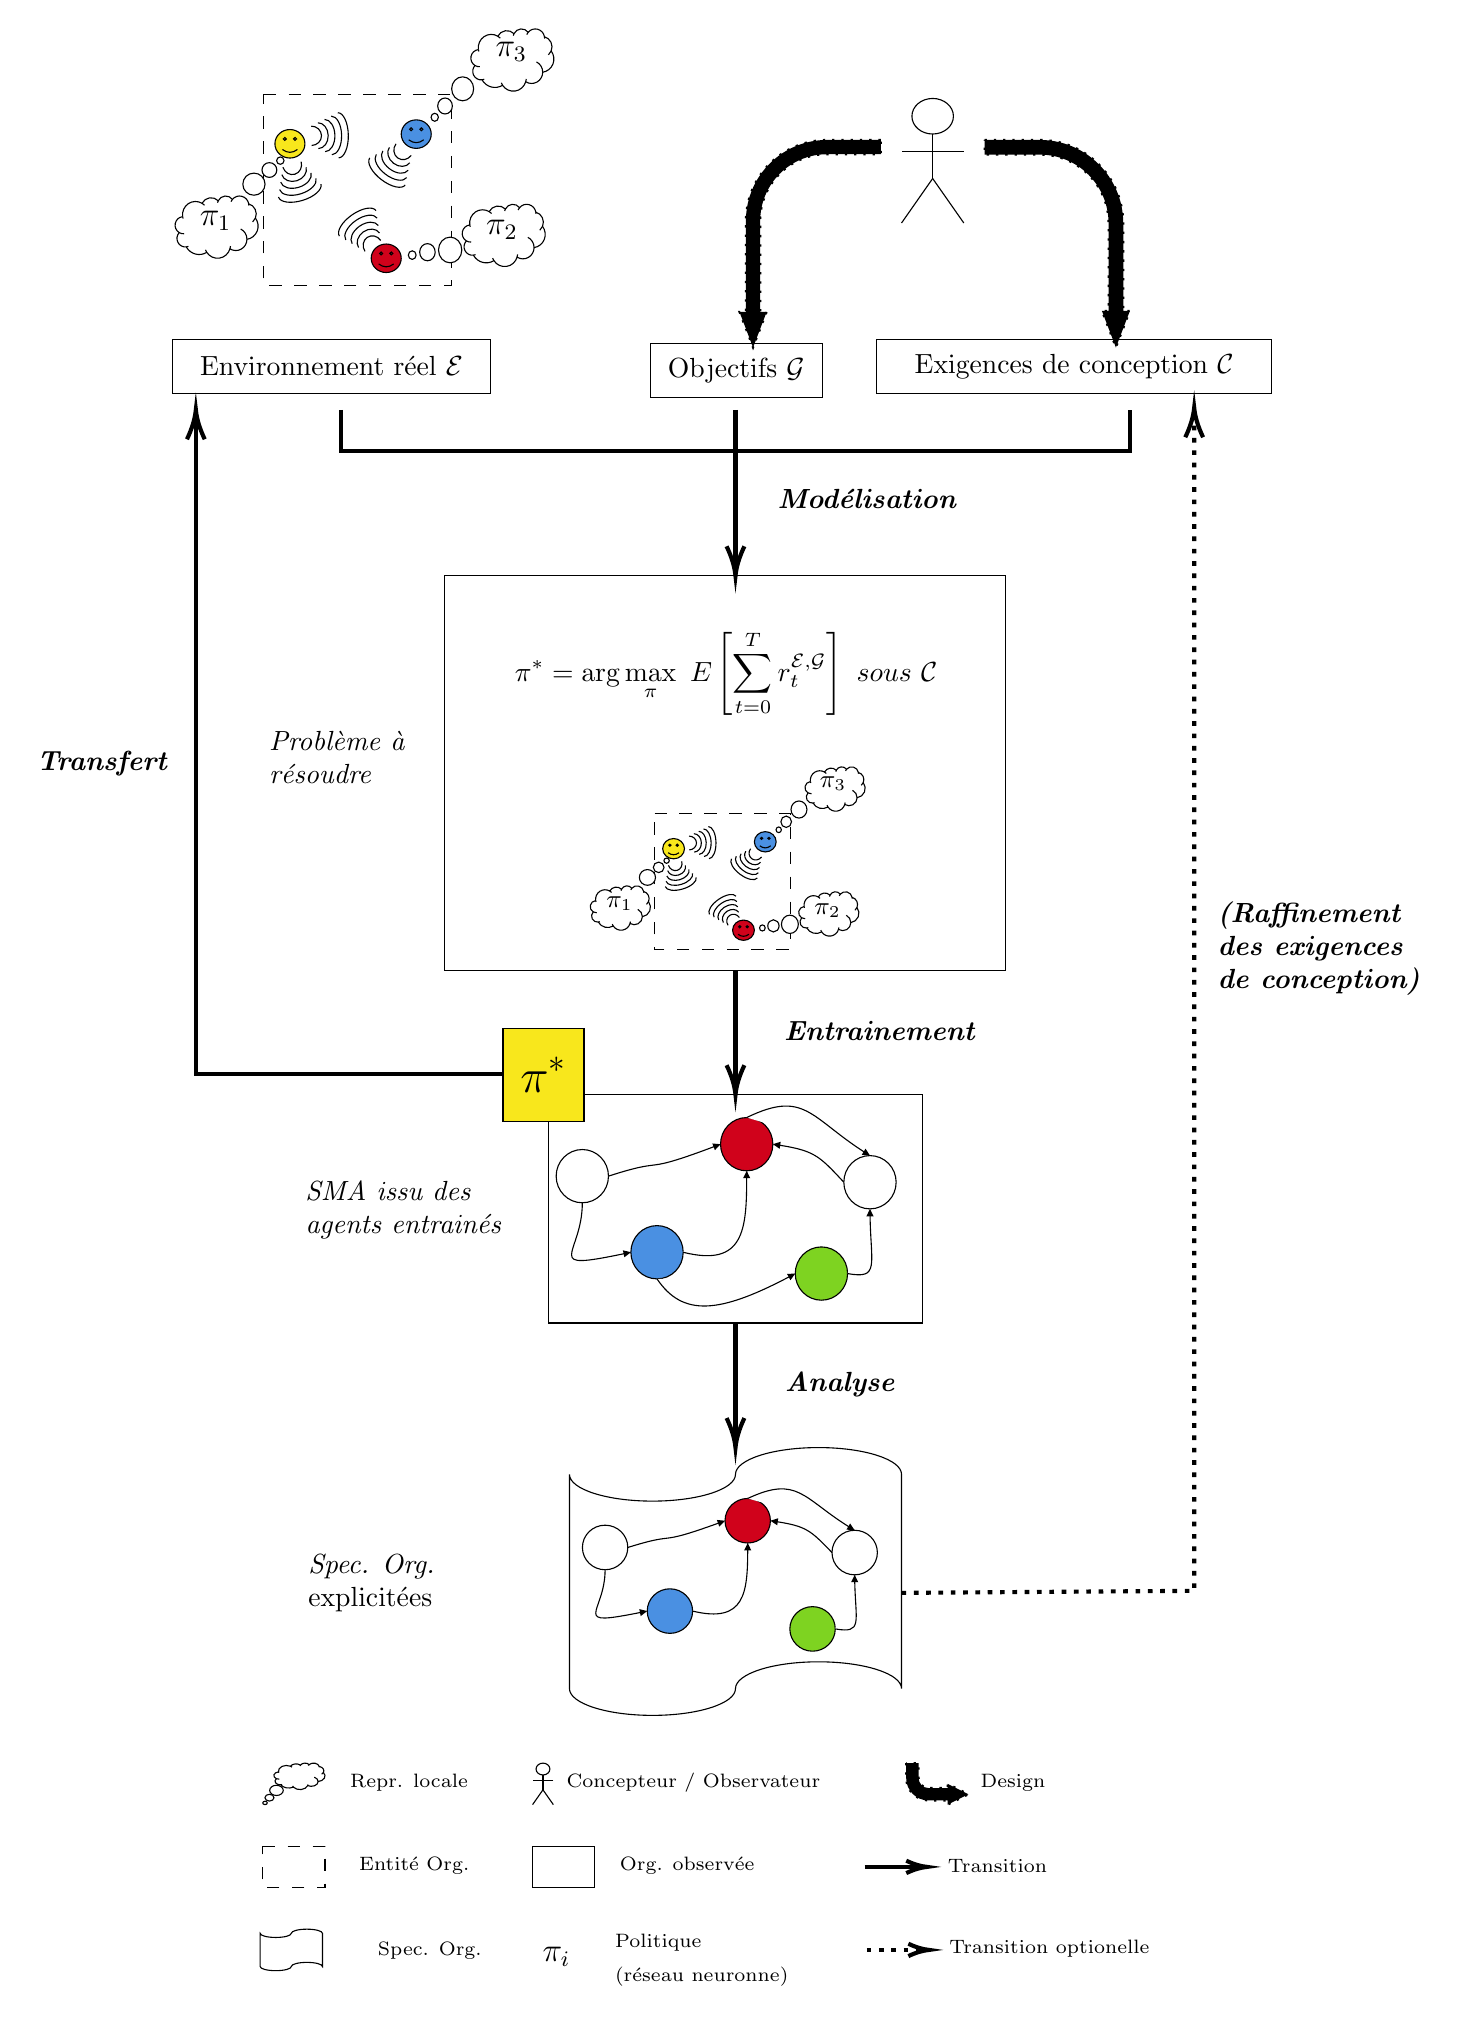
\begin{tikzpicture}[x=0.75pt,y=0.75pt,yscale=-1,xscale=1]
    %uncomment if require: \path (0,3967); %set diagram left start at 0, and has height of 3967

    %Shape: Rectangle [id:dp39157960168103956] 
    \draw  [fill={rgb, 255:red, 255; green, 255; blue, 255 }  ,fill opacity=1 ] (269,3000.97) -- (449,3000.97) -- (449,3110.97) -- (269,3110.97) -- cycle ;
    %Shape: Ellipse [id:dp9935722033847372] 
    \draw  [fill={rgb, 255:red, 255; green, 255; blue, 255 }  ,fill opacity=1 ] (272.6,3040.2) .. controls (272.6,3033.11) and (278.24,3027.37) .. (285.2,3027.37) .. controls (292.16,3027.37) and (297.8,3033.11) .. (297.8,3040.2) .. controls (297.8,3047.29) and (292.16,3053.03) .. (285.2,3053.03) .. controls (278.24,3053.03) and (272.6,3047.29) .. (272.6,3040.2) -- cycle ;
    %Shape: Ellipse [id:dp10593098470820161] 
    \draw  [fill={rgb, 255:red, 74; green, 144; blue, 226 }  ,fill opacity=1 ] (308.6,3076.87) .. controls (308.6,3069.78) and (314.24,3064.03) .. (321.2,3064.03) .. controls (328.16,3064.03) and (333.8,3069.78) .. (333.8,3076.87) .. controls (333.8,3083.96) and (328.16,3089.7) .. (321.2,3089.7) .. controls (314.24,3089.7) and (308.6,3083.96) .. (308.6,3076.87) -- cycle ;
    %Shape: Ellipse [id:dp9599003870836138] 
    \draw  [fill={rgb, 255:red, 208; green, 2; blue, 27 }  ,fill opacity=1 ] (351.8,3024.8) .. controls (351.8,3017.71) and (357.44,3011.97) .. (364.4,3011.97) .. controls (371.36,3011.97) and (377,3017.71) .. (377,3024.8) .. controls (377,3031.89) and (371.36,3037.63) .. (364.4,3037.63) .. controls (357.44,3037.63) and (351.8,3031.89) .. (351.8,3024.8) -- cycle ;
    %Shape: Ellipse [id:dp6518763640259156] 
    \draw  [fill={rgb, 255:red, 255; green, 255; blue, 255 }  ,fill opacity=1 ] (411.2,3043.13) .. controls (411.2,3036.05) and (416.84,3030.3) .. (423.8,3030.3) .. controls (430.76,3030.3) and (436.4,3036.05) .. (436.4,3043.13) .. controls (436.4,3050.22) and (430.76,3055.97) .. (423.8,3055.97) .. controls (416.84,3055.97) and (411.2,3050.22) .. (411.2,3043.13) -- cycle ;
    %Shape: Ellipse [id:dp9715345706408867] 
    \draw  [fill={rgb, 255:red, 126; green, 211; blue, 33 }  ,fill opacity=1 ] (387.8,3087.13) .. controls (387.8,3080.05) and (393.44,3074.3) .. (400.4,3074.3) .. controls (407.36,3074.3) and (413,3080.05) .. (413,3087.13) .. controls (413,3094.22) and (407.36,3099.97) .. (400.4,3099.97) .. controls (393.44,3099.97) and (387.8,3094.22) .. (387.8,3087.13) -- cycle ;
    %Curve Lines [id:da883230177824456] 
    \draw [fill={rgb, 255:red, 255; green, 255; blue, 255 }  ,fill opacity=1 ]   (297.8,3040.2) .. controls (327.79,3030.5) and (311.1,3040.17) .. (349.39,3025.72) ;
    \draw [shift={(351.8,3024.8)}, rotate = 159.15] [fill={rgb, 255:red, 0; green, 0; blue, 0 }  ][line width=0.08]  [draw opacity=0] (3.57,-1.72) -- (0,0) -- (3.57,1.72) -- cycle    ;
    %Curve Lines [id:da5139621017700224] 
    \draw [fill={rgb, 255:red, 255; green, 255; blue, 255 }  ,fill opacity=1 ]   (333.8,3076.87) .. controls (363.33,3084.3) and (364.36,3065.78) .. (364.4,3040.42) ;
    \draw [shift={(364.4,3037.63)}, rotate = 90] [fill={rgb, 255:red, 0; green, 0; blue, 0 }  ][line width=0.08]  [draw opacity=0] (3.57,-1.72) -- (0,0) -- (3.57,1.72) -- cycle    ;
    %Curve Lines [id:da31142570739384423] 
    \draw [fill={rgb, 255:red, 255; green, 255; blue, 255 }  ,fill opacity=1 ]   (411.2,3043.13) .. controls (399.23,3030.25) and (397.01,3027.95) .. (379.84,3025.23) ;
    \draw [shift={(377,3024.8)}, rotate = 8.43] [fill={rgb, 255:red, 0; green, 0; blue, 0 }  ][line width=0.08]  [draw opacity=0] (3.57,-1.72) -- (0,0) -- (3.57,1.72) -- cycle    ;
    %Curve Lines [id:da6742560121764545] 
    \draw [fill={rgb, 255:red, 255; green, 255; blue, 255 }  ,fill opacity=1 ]   (413,3087.13) .. controls (428.63,3089.97) and (424.15,3083.24) .. (423.82,3058.71) ;
    \draw [shift={(423.8,3055.97)}, rotate = 90] [fill={rgb, 255:red, 0; green, 0; blue, 0 }  ][line width=0.08]  [draw opacity=0] (3.57,-1.72) -- (0,0) -- (3.57,1.72) -- cycle    ;
    %Curve Lines [id:da9202599565974993] 
    \draw [fill={rgb, 255:red, 255; green, 255; blue, 255 }  ,fill opacity=1 ]   (285.2,3053.03) .. controls (285.2,3078.55) and (264.46,3086.1) .. (305.98,3077.42) ;
    \draw [shift={(308.6,3076.87)}, rotate = 168.04] [fill={rgb, 255:red, 0; green, 0; blue, 0 }  ][line width=0.08]  [draw opacity=0] (3.57,-1.72) -- (0,0) -- (3.57,1.72) -- cycle    ;
    %Curve Lines [id:da7585089826746155] 
    \draw [fill={rgb, 255:red, 255; green, 255; blue, 255 }  ,fill opacity=1 ]   (321.2,3089.7) .. controls (333.55,3108.03) and (351.08,3106.63) .. (385.66,3088.28) ;
    \draw [shift={(387.8,3087.13)}, rotate = 151.64] [fill={rgb, 255:red, 0; green, 0; blue, 0 }  ][line width=0.08]  [draw opacity=0] (3.57,-1.72) -- (0,0) -- (3.57,1.72) -- cycle    ;
    %Curve Lines [id:da9055022962664225] 
    \draw [fill={rgb, 255:red, 255; green, 255; blue, 255 }  ,fill opacity=1 ]   (364.4,3011.97) .. controls (392.34,2998.45) and (394.87,3011.85) .. (421.28,3028.73) ;
    \draw [shift={(423.8,3030.3)}, rotate = 211.43] [fill={rgb, 255:red, 0; green, 0; blue, 0 }  ][line width=0.08]  [draw opacity=0] (3.57,-1.72) -- (0,0) -- (3.57,1.72) -- cycle    ;
    %Shape: Rectangle [id:dp1660844159337831] 
    \draw  [dash pattern={on 4.5pt off 4.5pt}] (319.98,2865.49) -- (385.59,2865.49) -- (385.59,2930.97) -- (319.98,2930.97) -- cycle ;
    %Shape: Smiley Face [id:dp8672473520454604] 
    \draw  [fill={rgb, 255:red, 248; green, 231; blue, 28 }  ,fill opacity=1 ] (323.92,2882.43) .. controls (323.92,2879.73) and (326.27,2877.54) .. (329.17,2877.54) .. controls (332.07,2877.54) and (334.42,2879.73) .. (334.42,2882.43) .. controls (334.42,2885.13) and (332.07,2887.31) .. (329.17,2887.31) .. controls (326.27,2887.31) and (323.92,2885.13) .. (323.92,2882.43) -- cycle ; \draw  [fill={rgb, 255:red, 248; green, 231; blue, 28 }  ,fill opacity=1 ] (326.86,2880.76) .. controls (326.86,2880.49) and (327.1,2880.27) .. (327.39,2880.27) .. controls (327.68,2880.27) and (327.91,2880.49) .. (327.91,2880.76) .. controls (327.91,2881.03) and (327.68,2881.25) .. (327.39,2881.25) .. controls (327.1,2881.25) and (326.86,2881.03) .. (326.86,2880.76) -- cycle ; \draw  [fill={rgb, 255:red, 248; green, 231; blue, 28 }  ,fill opacity=1 ] (330.43,2880.76) .. controls (330.43,2880.49) and (330.66,2880.27) .. (330.95,2880.27) .. controls (331.24,2880.27) and (331.48,2880.49) .. (331.48,2880.76) .. controls (331.48,2881.03) and (331.24,2881.25) .. (330.95,2881.25) .. controls (330.66,2881.25) and (330.43,2881.03) .. (330.43,2880.76) -- cycle ; \draw   (326.55,2884.38) .. controls (328.3,2885.68) and (330.04,2885.68) .. (331.79,2884.38) ;
    %Shape: Arc [id:dp991830891477531] 
    \draw  [draw opacity=0] (340.03,2896.26) .. controls (340.03,2896.26) and (340.03,2896.26) .. (340.03,2896.26) .. controls (340.58,2898.12) and (337.71,2900.62) .. (333.6,2901.84) .. controls (329.5,2903.07) and (325.72,2902.55) .. (325.17,2900.69) -- (332.6,2898.48) -- cycle ; \draw   (340.03,2896.26) .. controls (340.03,2896.26) and (340.03,2896.26) .. (340.03,2896.26) .. controls (340.58,2898.12) and (337.71,2900.62) .. (333.6,2901.84) .. controls (329.5,2903.07) and (325.72,2902.55) .. (325.17,2900.69) ;
    %Shape: Arc [id:dp15270734978357758] 
    \draw  [draw opacity=0] (338.29,2894.33) .. controls (338.29,2894.33) and (338.29,2894.33) .. (338.29,2894.33) .. controls (338.85,2896.19) and (336.45,2898.55) .. (332.93,2899.6) .. controls (329.41,2900.65) and (326.11,2899.99) .. (325.55,2898.13) -- (331.92,2896.23) -- cycle ; \draw   (338.29,2894.33) .. controls (338.29,2894.33) and (338.29,2894.33) .. (338.29,2894.33) .. controls (338.85,2896.19) and (336.45,2898.55) .. (332.93,2899.6) .. controls (329.41,2900.65) and (326.11,2899.99) .. (325.55,2898.13) ;
    %Shape: Arc [id:dp4538189986822303] 
    \draw  [draw opacity=0] (336.56,2892.4) .. controls (336.56,2892.4) and (336.56,2892.4) .. (336.56,2892.4) .. controls (337.12,2894.26) and (335.19,2896.48) .. (332.26,2897.35) .. controls (329.33,2898.23) and (326.5,2897.43) .. (325.94,2895.57) -- (331.25,2893.99) -- cycle ; \draw   (336.56,2892.4) .. controls (336.56,2892.4) and (336.56,2892.4) .. (336.56,2892.4) .. controls (337.12,2894.26) and (335.19,2896.48) .. (332.26,2897.35) .. controls (329.33,2898.23) and (326.5,2897.43) .. (325.94,2895.57) ;
    %Shape: Arc [id:dp15781801722963062] 
    \draw  [draw opacity=0] (334.83,2890.48) .. controls (334.83,2890.48) and (334.83,2890.48) .. (334.83,2890.48) .. controls (335.38,2892.34) and (333.93,2894.41) .. (331.59,2895.11) .. controls (329.24,2895.81) and (326.89,2894.87) .. (326.33,2893.01) -- (330.58,2891.74) -- cycle ; \draw   (334.83,2890.48) .. controls (334.83,2890.48) and (334.83,2890.48) .. (334.83,2890.48) .. controls (335.38,2892.34) and (333.93,2894.41) .. (331.59,2895.11) .. controls (329.24,2895.81) and (326.89,2894.87) .. (326.33,2893.01) ;
    %Shape: Arc [id:dp647877332552287] 
    \draw  [draw opacity=0] (333.09,2888.55) .. controls (333.09,2888.55) and (333.09,2888.55) .. (333.09,2888.55) .. controls (333.65,2890.41) and (332.67,2892.34) .. (330.92,2892.87) .. controls (329.16,2893.39) and (327.28,2892.31) .. (326.72,2890.45) -- (329.91,2889.5) -- cycle ; \draw   (333.09,2888.55) .. controls (333.09,2888.55) and (333.09,2888.55) .. (333.09,2888.55) .. controls (333.65,2890.41) and (332.67,2892.34) .. (330.92,2892.87) .. controls (329.16,2893.39) and (327.28,2892.31) .. (326.72,2890.45) ;

    %Shape: Arc [id:dp12725807408272582] 
    \draw  [draw opacity=0] (345.93,2871.77) .. controls (345.93,2871.77) and (345.93,2871.77) .. (345.93,2871.77) .. controls (345.93,2871.77) and (345.93,2871.77) .. (345.93,2871.77) .. controls (347.87,2871.73) and (349.51,2875.16) .. (349.6,2879.44) .. controls (349.68,2883.71) and (348.17,2887.21) .. (346.23,2887.25) -- (346.08,2879.51) -- cycle ; \draw   (345.93,2871.77) .. controls (345.93,2871.77) and (345.93,2871.77) .. (345.93,2871.77) .. controls (345.93,2871.77) and (345.93,2871.77) .. (345.93,2871.77) .. controls (347.87,2871.73) and (349.51,2875.16) .. (349.6,2879.44) .. controls (349.68,2883.71) and (348.17,2887.21) .. (346.23,2887.25) ;
    %Shape: Arc [id:dp0663511362149849] 
    \draw  [draw opacity=0] (343.6,2872.92) .. controls (343.6,2872.92) and (343.6,2872.92) .. (343.6,2872.92) .. controls (345.54,2872.88) and (347.18,2875.82) .. (347.25,2879.48) .. controls (347.32,2883.15) and (345.81,2886.15) .. (343.86,2886.19) -- (343.73,2879.55) -- cycle ; \draw   (343.6,2872.92) .. controls (343.6,2872.92) and (343.6,2872.92) .. (343.6,2872.92) .. controls (345.54,2872.88) and (347.18,2875.82) .. (347.25,2879.48) .. controls (347.32,2883.15) and (345.81,2886.15) .. (343.86,2886.19) ;
    %Shape: Arc [id:dp5596459802099086] 
    \draw  [draw opacity=0] (341.28,2874.07) .. controls (341.28,2874.07) and (341.28,2874.07) .. (341.28,2874.07) .. controls (343.22,2874.03) and (344.84,2876.48) .. (344.9,2879.53) .. controls (344.97,2882.58) and (343.44,2885.09) .. (341.49,2885.13) -- (341.38,2879.6) -- cycle ; \draw   (341.28,2874.07) .. controls (341.28,2874.07) and (341.28,2874.07) .. (341.28,2874.07) .. controls (343.22,2874.03) and (344.84,2876.48) .. (344.9,2879.53) .. controls (344.97,2882.58) and (343.44,2885.09) .. (341.49,2885.13) ;
    %Shape: Arc [id:dp939679467729508] 
    \draw  [draw opacity=0] (338.95,2875.22) .. controls (338.95,2875.22) and (338.95,2875.22) .. (338.95,2875.22) .. controls (340.9,2875.18) and (342.51,2877.13) .. (342.56,2879.58) .. controls (342.61,2882.02) and (341.07,2884.03) .. (339.13,2884.07) -- (339.04,2879.65) -- cycle ; \draw   (338.95,2875.22) .. controls (338.95,2875.22) and (338.95,2875.22) .. (338.95,2875.22) .. controls (340.9,2875.18) and (342.51,2877.13) .. (342.56,2879.58) .. controls (342.61,2882.02) and (341.07,2884.03) .. (339.13,2884.07) ;
    %Shape: Arc [id:dp4187174998399785] 
    \draw  [draw opacity=0] (336.63,2876.37) .. controls (336.63,2876.37) and (336.63,2876.37) .. (336.63,2876.37) .. controls (338.57,2876.34) and (340.18,2877.79) .. (340.21,2879.62) .. controls (340.25,2881.45) and (338.7,2882.97) .. (336.76,2883.01) -- (336.69,2879.69) -- cycle ; \draw   (336.63,2876.37) .. controls (336.63,2876.37) and (336.63,2876.37) .. (336.63,2876.37) .. controls (338.57,2876.34) and (340.18,2877.79) .. (340.21,2879.62) .. controls (340.25,2881.45) and (338.7,2882.97) .. (336.76,2883.01) ;

    %Shape: Smiley Face [id:dp2664344043944723] 
    \draw  [fill={rgb, 255:red, 208; green, 2; blue, 27 }  ,fill opacity=1 ] (357.6,2921.71) .. controls (357.6,2919.01) and (359.95,2916.82) .. (362.85,2916.82) .. controls (365.75,2916.82) and (368.1,2919.01) .. (368.1,2921.71) .. controls (368.1,2924.41) and (365.75,2926.6) .. (362.85,2926.6) .. controls (359.95,2926.6) and (357.6,2924.41) .. (357.6,2921.71) -- cycle ; \draw  [fill={rgb, 255:red, 208; green, 2; blue, 27 }  ,fill opacity=1 ] (360.54,2920.05) .. controls (360.54,2919.78) and (360.78,2919.56) .. (361.07,2919.56) .. controls (361.36,2919.56) and (361.59,2919.78) .. (361.59,2920.05) .. controls (361.59,2920.32) and (361.36,2920.54) .. (361.07,2920.54) .. controls (360.78,2920.54) and (360.54,2920.32) .. (360.54,2920.05) -- cycle ; \draw  [fill={rgb, 255:red, 208; green, 2; blue, 27 }  ,fill opacity=1 ] (364.11,2920.05) .. controls (364.11,2919.78) and (364.34,2919.56) .. (364.63,2919.56) .. controls (364.92,2919.56) and (365.16,2919.78) .. (365.16,2920.05) .. controls (365.16,2920.32) and (364.92,2920.54) .. (364.63,2920.54) .. controls (364.34,2920.54) and (364.11,2920.32) .. (364.11,2920.05) -- cycle ; \draw   (360.23,2923.67) .. controls (361.98,2924.97) and (363.72,2924.97) .. (365.47,2923.67) ;
    %Shape: Arc [id:dp7671134474873877] 
    \draw  [draw opacity=0] (346.47,2914.11) .. controls (346.47,2914.11) and (346.47,2914.11) .. (346.47,2914.11) .. controls (345.37,2912.51) and (347.34,2909.26) .. (350.88,2906.84) .. controls (354.41,2904.42) and (358.16,2903.76) .. (359.26,2905.36) -- (352.87,2909.74) -- cycle ; \draw   (346.47,2914.11) .. controls (346.47,2914.11) and (346.47,2914.11) .. (346.47,2914.11) .. controls (345.37,2912.51) and (347.34,2909.26) .. (350.88,2906.84) .. controls (354.41,2904.42) and (358.16,2903.76) .. (359.26,2905.36) ;
    %Shape: Arc [id:dp7465446437475772] 
    \draw  [draw opacity=0] (348.71,2915.42) .. controls (348.71,2915.42) and (348.71,2915.42) .. (348.71,2915.42) .. controls (347.61,2913.82) and (349.18,2910.84) .. (352.2,2908.77) .. controls (355.23,2906.7) and (358.58,2906.32) .. (359.68,2907.92) .. controls (359.68,2907.92) and (359.68,2907.92) .. (359.68,2907.92) -- (354.19,2911.67) -- cycle ; \draw   (348.71,2915.42) .. controls (348.71,2915.42) and (348.71,2915.42) .. (348.71,2915.42) .. controls (347.61,2913.82) and (349.18,2910.84) .. (352.2,2908.77) .. controls (355.23,2906.7) and (358.58,2906.32) .. (359.68,2907.92) .. controls (359.68,2907.92) and (359.68,2907.92) .. (359.68,2907.92) ;
    %Shape: Arc [id:dp9770041114548759] 
    \draw  [draw opacity=0] (350.95,2916.73) .. controls (350.95,2916.73) and (350.95,2916.73) .. (350.95,2916.73) .. controls (350.95,2916.73) and (350.95,2916.73) .. (350.95,2916.73) .. controls (349.85,2915.13) and (351.01,2912.43) .. (353.53,2910.7) .. controls (356.05,2908.98) and (358.99,2908.87) .. (360.09,2910.47) -- (355.52,2913.6) -- cycle ; \draw   (350.95,2916.73) .. controls (350.95,2916.73) and (350.95,2916.73) .. (350.95,2916.73) .. controls (350.95,2916.73) and (350.95,2916.73) .. (350.95,2916.73) .. controls (349.85,2915.13) and (351.01,2912.43) .. (353.53,2910.7) .. controls (356.05,2908.98) and (358.99,2908.87) .. (360.09,2910.47) ;
    %Shape: Arc [id:dp4418659452921887] 
    \draw  [draw opacity=0] (353.19,2918.03) .. controls (353.19,2918.03) and (353.19,2918.03) .. (353.19,2918.03) .. controls (353.19,2918.03) and (353.19,2918.03) .. (353.19,2918.03) .. controls (352.09,2916.43) and (352.84,2914.02) .. (354.86,2912.63) .. controls (356.88,2911.25) and (359.4,2911.43) .. (360.5,2913.03) -- (356.85,2915.53) -- cycle ; \draw   (353.19,2918.03) .. controls (353.19,2918.03) and (353.19,2918.03) .. (353.19,2918.03) .. controls (353.19,2918.03) and (353.19,2918.03) .. (353.19,2918.03) .. controls (352.09,2916.43) and (352.84,2914.02) .. (354.86,2912.63) .. controls (356.88,2911.25) and (359.4,2911.43) .. (360.5,2913.03) ;
    %Shape: Arc [id:dp6696566494284376] 
    \draw  [draw opacity=0] (355.43,2919.34) .. controls (355.43,2919.34) and (355.43,2919.34) .. (355.43,2919.34) .. controls (354.34,2917.74) and (354.67,2915.6) .. (356.18,2914.57) .. controls (357.7,2913.53) and (359.82,2913.99) .. (360.92,2915.59) -- (358.18,2917.46) -- cycle ; \draw   (355.43,2919.34) .. controls (355.43,2919.34) and (355.43,2919.34) .. (355.43,2919.34) .. controls (354.34,2917.74) and (354.67,2915.6) .. (356.18,2914.57) .. controls (357.7,2913.53) and (359.82,2913.99) .. (360.92,2915.59) ;

    %Shape: Smiley Face [id:dp09777682624392658] 
    \draw  [fill={rgb, 255:red, 74; green, 144; blue, 226 }  ,fill opacity=1 ] (368.1,2879.11) .. controls (368.1,2876.41) and (370.45,2874.22) .. (373.35,2874.22) .. controls (376.25,2874.22) and (378.6,2876.41) .. (378.6,2879.11) .. controls (378.6,2881.81) and (376.25,2884) .. (373.35,2884) .. controls (370.45,2884) and (368.1,2881.81) .. (368.1,2879.11) -- cycle ; \draw  [fill={rgb, 255:red, 74; green, 144; blue, 226 }  ,fill opacity=1 ] (371.04,2877.45) .. controls (371.04,2877.18) and (371.27,2876.96) .. (371.56,2876.96) .. controls (371.85,2876.96) and (372.09,2877.18) .. (372.09,2877.45) .. controls (372.09,2877.72) and (371.85,2877.93) .. (371.56,2877.93) .. controls (371.27,2877.93) and (371.04,2877.72) .. (371.04,2877.45) -- cycle ; \draw  [fill={rgb, 255:red, 74; green, 144; blue, 226 }  ,fill opacity=1 ] (374.61,2877.45) .. controls (374.61,2877.18) and (374.84,2876.96) .. (375.13,2876.96) .. controls (375.42,2876.96) and (375.66,2877.18) .. (375.66,2877.45) .. controls (375.66,2877.72) and (375.42,2877.93) .. (375.13,2877.93) .. controls (374.84,2877.93) and (374.61,2877.72) .. (374.61,2877.45) -- cycle ; \draw   (370.72,2881.06) .. controls (372.47,2882.37) and (374.22,2882.37) .. (375.97,2881.06) ;
    %Shape: Arc [id:dp7162316795920435] 
    \draw  [draw opacity=0] (369.5,2896.57) .. controls (368.33,2898.12) and (364.61,2897.3) .. (361.18,2894.74) .. controls (357.76,2892.18) and (355.92,2888.84) .. (357.09,2887.29) .. controls (357.09,2887.29) and (357.09,2887.29) .. (357.09,2887.29) -- (363.29,2891.93) -- cycle ; \draw   (369.5,2896.57) .. controls (368.33,2898.12) and (364.61,2897.3) .. (361.18,2894.74) .. controls (357.76,2892.18) and (355.92,2888.84) .. (357.09,2887.29) .. controls (357.09,2887.29) and (357.09,2887.29) .. (357.09,2887.29) ;
    %Shape: Arc [id:dp412134008181967] 
    \draw  [draw opacity=0] (370.02,2894.03) .. controls (370.02,2894.03) and (370.02,2894.03) .. (370.02,2894.03) .. controls (370.02,2894.03) and (370.02,2894.03) .. (370.02,2894.03) .. controls (368.86,2895.59) and (365.53,2895.06) .. (362.59,2892.87) .. controls (359.65,2890.67) and (358.22,2887.63) .. (359.38,2886.08) .. controls (359.38,2886.08) and (359.38,2886.08) .. (359.38,2886.08) -- (364.7,2890.06) -- cycle ; \draw   (370.02,2894.03) .. controls (370.02,2894.03) and (370.02,2894.03) .. (370.02,2894.03) .. controls (370.02,2894.03) and (370.02,2894.03) .. (370.02,2894.03) .. controls (368.86,2895.59) and (365.53,2895.06) .. (362.59,2892.87) .. controls (359.65,2890.67) and (358.22,2887.63) .. (359.38,2886.08) .. controls (359.38,2886.08) and (359.38,2886.08) .. (359.38,2886.08) ;
    %Shape: Arc [id:dp9457493036891829] 
    \draw  [draw opacity=0] (370.54,2891.5) .. controls (370.54,2891.5) and (370.54,2891.5) .. (370.54,2891.5) .. controls (370.54,2891.5) and (370.54,2891.5) .. (370.54,2891.5) .. controls (369.38,2893.05) and (366.45,2892.82) .. (364,2890.99) .. controls (361.55,2889.16) and (360.51,2886.42) .. (361.68,2884.87) -- (366.11,2888.18) -- cycle ; \draw   (370.54,2891.5) .. controls (370.54,2891.5) and (370.54,2891.5) .. (370.54,2891.5) .. controls (370.54,2891.5) and (370.54,2891.5) .. (370.54,2891.5) .. controls (369.38,2893.05) and (366.45,2892.82) .. (364,2890.99) .. controls (361.55,2889.16) and (360.51,2886.42) .. (361.68,2884.87) ;
    %Shape: Arc [id:dp6838488823519279] 
    \draw  [draw opacity=0] (371.06,2888.96) .. controls (371.06,2888.96) and (371.06,2888.96) .. (371.06,2888.96) .. controls (369.9,2890.51) and (367.36,2890.58) .. (365.41,2889.12) .. controls (363.45,2887.65) and (362.8,2885.21) .. (363.97,2883.65) -- (367.52,2886.31) -- cycle ; \draw   (371.06,2888.96) .. controls (371.06,2888.96) and (371.06,2888.96) .. (371.06,2888.96) .. controls (369.9,2890.51) and (367.36,2890.58) .. (365.41,2889.12) .. controls (363.45,2887.65) and (362.8,2885.21) .. (363.97,2883.65) ;
    %Shape: Arc [id:dp5242677755784311] 
    \draw  [draw opacity=0] (371.58,2886.42) .. controls (371.58,2886.42) and (371.58,2886.42) .. (371.58,2886.42) .. controls (371.58,2886.42) and (371.58,2886.42) .. (371.58,2886.42) .. controls (370.42,2887.97) and (368.28,2888.34) .. (366.81,2887.24) .. controls (365.34,2886.15) and (365.1,2884) .. (366.26,2882.44) -- (368.92,2884.43) -- cycle ; \draw   (371.58,2886.42) .. controls (371.58,2886.42) and (371.58,2886.42) .. (371.58,2886.42) .. controls (371.58,2886.42) and (371.58,2886.42) .. (371.58,2886.42) .. controls (370.42,2887.97) and (368.28,2888.34) .. (366.81,2887.24) .. controls (365.34,2886.15) and (365.1,2884) .. (366.26,2882.44) ;

    %Shape: Cloud [id:dp4236644517840452] 
    \draw  [fill={rgb, 255:red, 255; green, 255; blue, 255 }  ,fill opacity=1 ] (291.64,2907.38) .. controls (291.41,2905.65) and (292.18,2903.95) .. (293.62,2902.98) .. controls (295.06,2902.02) and (296.93,2901.96) .. (298.43,2902.84) .. controls (298.96,2901.84) and (299.93,2901.15) .. (301.05,2900.98) .. controls (302.16,2900.81) and (303.29,2901.17) .. (304.1,2901.97) .. controls (304.55,2901.06) and (305.44,2900.45) .. (306.45,2900.35) .. controls (307.45,2900.26) and (308.44,2900.69) .. (309.05,2901.5) .. controls (309.87,2900.54) and (311.17,2900.13) .. (312.39,2900.46) .. controls (313.61,2900.79) and (314.53,2901.79) .. (314.75,2903.03) .. controls (315.75,2903.3) and (316.58,2904) .. (317.03,2904.93) .. controls (317.48,2905.87) and (317.51,2906.96) .. (317.1,2907.92) .. controls (318.08,2909.2) and (318.31,2910.91) .. (317.7,2912.41) .. controls (317.1,2913.91) and (315.74,2914.98) .. (314.14,2915.2) .. controls (314.12,2916.61) and (313.35,2917.9) .. (312.12,2918.58) .. controls (310.89,2919.26) and (309.39,2919.22) .. (308.2,2918.47) .. controls (307.69,2920.16) and (306.26,2921.4) .. (304.52,2921.66) .. controls (302.79,2921.92) and (301.06,2921.15) .. (300.09,2919.68) .. controls (298.89,2920.41) and (297.46,2920.61) .. (296.11,2920.26) .. controls (294.76,2919.91) and (293.61,2919.02) .. (292.92,2917.81) .. controls (291.7,2917.95) and (290.52,2917.32) .. (289.97,2916.22) .. controls (289.41,2915.13) and (289.6,2913.8) .. (290.44,2912.9) .. controls (289.35,2912.26) and (288.8,2910.99) .. (289.07,2909.74) .. controls (289.33,2908.5) and (290.36,2907.57) .. (291.62,2907.44) ; \draw   (290.44,2912.9) .. controls (290.96,2913.21) and (291.55,2913.34) .. (292.14,2913.3)(292.92,2917.81) .. controls (293.18,2917.78) and (293.43,2917.72) .. (293.67,2917.62)(300.09,2919.68) .. controls (299.91,2919.41) and (299.76,2919.13) .. (299.64,2918.82)(308.2,2918.47) .. controls (308.29,2918.17) and (308.35,2917.85) .. (308.38,2917.53)(314.14,2915.2) .. controls (314.15,2913.71) and (313.3,2912.33) .. (311.95,2911.68)(317.1,2907.92) .. controls (316.88,2908.43) and (316.55,2908.88) .. (316.13,2909.24)(314.75,2903.03) .. controls (314.79,2903.23) and (314.8,2903.44) .. (314.8,2903.65)(309.05,2901.5) .. controls (308.85,2901.74) and (308.68,2902.01) .. (308.56,2902.3)(304.1,2901.97) .. controls (303.99,2902.19) and (303.91,2902.42) .. (303.86,2902.66)(298.43,2902.84) .. controls (298.74,2903.03) and (299.04,2903.25) .. (299.3,2903.51)(291.64,2907.38) .. controls (291.67,2907.61) and (291.73,2907.85) .. (291.79,2908.08) ;
    %Shape: Cloud [id:dp9261610463414396] 
    \draw  [fill={rgb, 255:red, 255; green, 255; blue, 255 }  ,fill opacity=1 ] (395.1,2850.04) .. controls (394.87,2848.32) and (395.64,2846.61) .. (397.08,2845.65) .. controls (398.52,2844.68) and (400.39,2844.63) .. (401.89,2845.51) .. controls (402.42,2844.51) and (403.39,2843.82) .. (404.5,2843.64) .. controls (405.62,2843.47) and (406.75,2843.84) .. (407.56,2844.63) .. controls (408.01,2843.73) and (408.9,2843.12) .. (409.91,2843.02) .. controls (410.91,2842.92) and (411.9,2843.36) .. (412.51,2844.16) .. controls (413.33,2843.2) and (414.63,2842.8) .. (415.85,2843.12) .. controls (417.06,2843.45) and (417.98,2844.45) .. (418.21,2845.69) .. controls (419.21,2845.97) and (420.04,2846.66) .. (420.49,2847.6) .. controls (420.94,2848.54) and (420.97,2849.62) .. (420.56,2850.58) .. controls (421.54,2851.87) and (421.77,2853.58) .. (421.16,2855.08) .. controls (420.55,2856.58) and (419.2,2857.64) .. (417.6,2857.87) .. controls (417.58,2859.28) and (416.81,2860.57) .. (415.58,2861.25) .. controls (414.35,2861.93) and (412.85,2861.88) .. (411.65,2861.14) .. controls (411.15,2862.82) and (409.72,2864.06) .. (407.98,2864.32) .. controls (406.25,2864.58) and (404.52,2863.81) .. (403.55,2862.35) .. controls (402.35,2863.07) and (400.92,2863.28) .. (399.57,2862.93) .. controls (398.22,2862.57) and (397.07,2861.69) .. (396.38,2860.47) .. controls (395.16,2860.62) and (393.98,2859.98) .. (393.43,2858.89) .. controls (392.87,2857.79) and (393.06,2856.46) .. (393.9,2855.57) .. controls (392.81,2854.93) and (392.26,2853.65) .. (392.53,2852.41) .. controls (392.79,2851.17) and (393.82,2850.24) .. (395.08,2850.11) ; \draw   (393.9,2855.57) .. controls (394.42,2855.87) and (395.01,2856.01) .. (395.6,2855.96)(396.38,2860.47) .. controls (396.64,2860.44) and (396.89,2860.38) .. (397.12,2860.28)(403.55,2862.35) .. controls (403.37,2862.08) and (403.22,2861.79) .. (403.1,2861.49)(411.65,2861.14) .. controls (411.75,2860.83) and (411.81,2860.51) .. (411.83,2860.19)(417.59,2857.87) .. controls (417.61,2856.37) and (416.76,2855) .. (415.41,2854.34)(420.56,2850.58) .. controls (420.34,2851.09) and (420.01,2851.54) .. (419.59,2851.9)(418.21,2845.69) .. controls (418.25,2845.9) and (418.26,2846.11) .. (418.26,2846.32)(412.51,2844.16) .. controls (412.31,2844.4) and (412.14,2844.67) .. (412.01,2844.96)(407.56,2844.63) .. controls (407.45,2844.85) and (407.37,2845.08) .. (407.32,2845.32)(401.89,2845.51) .. controls (402.2,2845.69) and (402.5,2845.92) .. (402.76,2846.18)(395.1,2850.04) .. controls (395.13,2850.28) and (395.18,2850.51) .. (395.25,2850.74) ;
    %Shape: Ellipse [id:dp38327597242410594] 
    \draw  [fill={rgb, 255:red, 255; green, 255; blue, 255 }  ,fill opacity=1 ] (380.86,2869.46) .. controls (380.86,2867.95) and (382.01,2866.72) .. (383.43,2866.72) .. controls (384.84,2866.72) and (385.99,2867.95) .. (385.99,2869.46) .. controls (385.99,2870.97) and (384.84,2872.2) .. (383.43,2872.2) .. controls (382.01,2872.2) and (380.86,2870.97) .. (380.86,2869.46) -- cycle ;
    %Shape: Ellipse [id:dp0569021122146276] 
    \draw  [fill={rgb, 255:red, 255; green, 255; blue, 255 }  ,fill opacity=1 ] (378.54,2873.33) .. controls (378.54,2872.57) and (379.12,2871.96) .. (379.82,2871.96) .. controls (380.53,2871.96) and (381.11,2872.57) .. (381.11,2873.33) .. controls (381.11,2874.09) and (380.53,2874.7) .. (379.82,2874.7) .. controls (379.12,2874.7) and (378.54,2874.09) .. (378.54,2873.33) -- cycle ;
    %Shape: Ellipse [id:dp908037679999253] 
    \draw  [fill={rgb, 255:red, 255; green, 255; blue, 255 }  ,fill opacity=1 ] (319.4,2891.43) .. controls (319.4,2890.03) and (320.56,2888.9) .. (321.99,2888.9) .. controls (323.42,2888.9) and (324.58,2890.03) .. (324.58,2891.43) .. controls (324.58,2892.82) and (323.42,2893.95) .. (321.99,2893.95) .. controls (320.56,2893.95) and (319.4,2892.82) .. (319.4,2891.43) -- cycle ;
    %Shape: Ellipse [id:dp7926420178535974] 
    \draw  [fill={rgb, 255:red, 255; green, 255; blue, 255 }  ,fill opacity=1 ] (312.69,2896.28) .. controls (312.69,2894.19) and (314.43,2892.49) .. (316.58,2892.49) .. controls (318.72,2892.49) and (320.46,2894.19) .. (320.46,2896.28) .. controls (320.46,2898.38) and (318.72,2900.07) .. (316.58,2900.07) .. controls (314.43,2900.07) and (312.69,2898.38) .. (312.69,2896.28) -- cycle ;
    %Shape: Ellipse [id:dp884513706406913] 
    \draw  [fill={rgb, 255:red, 255; green, 255; blue, 255 }  ,fill opacity=1 ] (324.52,2888.2) .. controls (324.52,2887.51) and (325.1,2886.94) .. (325.81,2886.94) .. controls (326.53,2886.94) and (327.11,2887.51) .. (327.11,2888.2) .. controls (327.11,2888.9) and (326.53,2889.47) .. (325.81,2889.47) .. controls (325.1,2889.47) and (324.52,2888.9) .. (324.52,2888.2) -- cycle ;
    %Shape: Ellipse [id:dp045097605817289055] 
    \draw  [fill={rgb, 255:red, 255; green, 255; blue, 255 }  ,fill opacity=1 ] (385.75,2863.56) .. controls (385.75,2861.29) and (387.47,2859.45) .. (389.59,2859.45) .. controls (391.71,2859.45) and (393.43,2861.29) .. (393.43,2863.56) .. controls (393.43,2865.83) and (391.71,2867.67) .. (389.59,2867.67) .. controls (387.47,2867.67) and (385.75,2865.83) .. (385.75,2863.56) -- cycle ;
    %Shape: Ellipse [id:dp34409865082548896] 
    \draw  [fill={rgb, 255:red, 255; green, 255; blue, 255 }  ,fill opacity=1 ] (381.14,2918.86) .. controls (381.14,2916.42) and (382.97,2914.45) .. (385.22,2914.45) .. controls (387.47,2914.45) and (389.29,2916.42) .. (389.29,2918.86) .. controls (389.29,2921.29) and (387.47,2923.27) .. (385.22,2923.27) .. controls (382.97,2923.27) and (381.14,2921.29) .. (381.14,2918.86) -- cycle ;
    %Shape: Ellipse [id:dp7946586129033605] 
    \draw  [fill={rgb, 255:red, 255; green, 255; blue, 255 }  ,fill opacity=1 ] (374.56,2919.62) .. controls (374.56,2918) and (375.77,2916.68) .. (377.27,2916.68) .. controls (378.77,2916.68) and (379.99,2918) .. (379.99,2919.62) .. controls (379.99,2921.25) and (378.77,2922.56) .. (377.27,2922.56) .. controls (375.77,2922.56) and (374.56,2921.25) .. (374.56,2919.62) -- cycle ;
    %Shape: Ellipse [id:dp8588991503220264] 
    \draw  [fill={rgb, 255:red, 255; green, 255; blue, 255 }  ,fill opacity=1 ] (370.59,2920.62) .. controls (370.59,2919.81) and (371.2,2919.15) .. (371.95,2919.15) .. controls (372.7,2919.15) and (373.31,2919.81) .. (373.31,2920.62) .. controls (373.31,2921.43) and (372.7,2922.09) .. (371.95,2922.09) .. controls (371.2,2922.09) and (370.59,2921.43) .. (370.59,2920.62) -- cycle ;
    %Shape: Cloud [id:dp5704725396428417] 
    \draw  [fill={rgb, 255:red, 255; green, 255; blue, 255 }  ,fill opacity=1 ] (392.08,2910.23) .. controls (391.84,2908.5) and (392.61,2906.8) .. (394.06,2905.83) .. controls (395.5,2904.87) and (397.37,2904.81) .. (398.86,2905.69) .. controls (399.39,2904.69) and (400.36,2904) .. (401.48,2903.83) .. controls (402.6,2903.65) and (403.73,2904.02) .. (404.54,2904.82) .. controls (404.99,2903.91) and (405.87,2903.3) .. (406.88,2903.2) .. controls (407.89,2903.11) and (408.88,2903.54) .. (409.49,2904.35) .. controls (410.31,2903.39) and (411.6,2902.98) .. (412.82,2903.31) .. controls (414.04,2903.63) and (414.96,2904.64) .. (415.19,2905.88) .. controls (416.19,2906.15) and (417.02,2906.85) .. (417.47,2907.78) .. controls (417.92,2908.72) and (417.94,2909.81) .. (417.54,2910.76) .. controls (418.52,2912.05) and (418.75,2913.76) .. (418.14,2915.26) .. controls (417.53,2916.76) and (416.17,2917.82) .. (414.57,2918.05) .. controls (414.56,2919.46) and (413.79,2920.75) .. (412.56,2921.43) .. controls (411.33,2922.11) and (409.82,2922.07) .. (408.63,2921.32) .. controls (408.12,2923.01) and (406.69,2924.25) .. (404.96,2924.51) .. controls (403.23,2924.77) and (401.5,2924) .. (400.52,2922.53) .. controls (399.33,2923.26) and (397.9,2923.46) .. (396.55,2923.11) .. controls (395.2,2922.76) and (394.05,2921.87) .. (393.36,2920.66) .. controls (392.14,2920.8) and (390.96,2920.17) .. (390.4,2919.07) .. controls (389.85,2917.97) and (390.04,2916.65) .. (390.88,2915.75) .. controls (389.79,2915.11) and (389.23,2913.84) .. (389.5,2912.59) .. controls (389.77,2911.35) and (390.8,2910.42) .. (392.05,2910.29) ; \draw   (390.88,2915.75) .. controls (391.39,2916.06) and (391.99,2916.19) .. (392.58,2916.15)(393.36,2920.66) .. controls (393.61,2920.63) and (393.86,2920.56) .. (394.1,2920.47)(400.52,2922.53) .. controls (400.34,2922.26) and (400.19,2921.97) .. (400.08,2921.67)(408.63,2921.32) .. controls (408.72,2921.01) and (408.78,2920.7) .. (408.81,2920.38)(414.57,2918.05) .. controls (414.58,2916.55) and (413.73,2915.18) .. (412.39,2914.53)(417.54,2910.76) .. controls (417.32,2911.27) and (416.98,2911.73) .. (416.56,2912.09)(415.19,2905.88) .. controls (415.22,2906.08) and (415.24,2906.29) .. (415.24,2906.5)(409.49,2904.35) .. controls (409.29,2904.59) and (409.12,2904.86) .. (408.99,2905.14)(404.54,2904.82) .. controls (404.43,2905.04) and (404.35,2905.27) .. (404.3,2905.51)(398.86,2905.69) .. controls (399.18,2905.88) and (399.47,2906.1) .. (399.74,2906.36)(392.08,2910.23) .. controls (392.11,2910.46) and (392.16,2910.7) .. (392.23,2910.93) ;
    %Shape: Rectangle [id:dp2824507959380417] 
    \draw   (219,2750.97) -- (489,2750.97) -- (489,2940.97) -- (219,2940.97) -- cycle ;
    %Flowchart: Punched Tape [id:dp9081855054145813] 
    \draw  [fill={rgb, 255:red, 255; green, 255; blue, 255 }  ,fill opacity=1 ] (279,3183.87) .. controls (279,3191) and (296.91,3196.77) .. (319,3196.77) .. controls (341.09,3196.77) and (359,3191) .. (359,3183.87) .. controls (359,3176.74) and (376.91,3170.97) .. (399,3170.97) .. controls (421.09,3170.97) and (439,3176.74) .. (439,3183.87) -- (439,3287.1) .. controls (439,3279.97) and (421.09,3274.19) .. (399,3274.19) .. controls (376.91,3274.19) and (359,3279.97) .. (359,3287.1) .. controls (359,3294.22) and (341.09,3300) .. (319,3300) .. controls (296.91,3300) and (279,3294.22) .. (279,3287.1) -- cycle ;
    %Shape: Ellipse [id:dp16129214012888815] 
    \draw  [fill={rgb, 255:red, 255; green, 255; blue, 255 }  ,fill opacity=1 ] (285.25,3219.1) .. controls (285.25,3213.17) and (290.14,3208.37) .. (296.18,3208.37) .. controls (302.22,3208.37) and (307.11,3213.17) .. (307.11,3219.1) .. controls (307.11,3225.02) and (302.22,3229.83) .. (296.18,3229.83) .. controls (290.14,3229.83) and (285.25,3225.02) .. (285.25,3219.1) -- cycle ;
    %Shape: Ellipse [id:dp46629806906917204] 
    \draw  [fill={rgb, 255:red, 74; green, 144; blue, 226 }  ,fill opacity=1 ] (316.48,3249.75) .. controls (316.48,3243.83) and (321.37,3239.02) .. (327.41,3239.02) .. controls (333.45,3239.02) and (338.34,3243.83) .. (338.34,3249.75) .. controls (338.34,3255.68) and (333.45,3260.48) .. (327.41,3260.48) .. controls (321.37,3260.48) and (316.48,3255.68) .. (316.48,3249.75) -- cycle ;
    %Shape: Ellipse [id:dp8639592543358846] 
    \draw  [fill={rgb, 255:red, 208; green, 2; blue, 27 }  ,fill opacity=1 ] (353.96,3206.22) .. controls (353.96,3200.3) and (358.85,3195.49) .. (364.89,3195.49) .. controls (370.93,3195.49) and (375.82,3200.3) .. (375.82,3206.22) .. controls (375.82,3212.15) and (370.93,3216.95) .. (364.89,3216.95) .. controls (358.85,3216.95) and (353.96,3212.15) .. (353.96,3206.22) -- cycle ;
    %Shape: Ellipse [id:dp0625434790011643] 
    \draw  [fill={rgb, 255:red, 255; green, 255; blue, 255 }  ,fill opacity=1 ] (405.5,3221.55) .. controls (405.5,3215.62) and (410.39,3210.82) .. (416.43,3210.82) .. controls (422.46,3210.82) and (427.36,3215.62) .. (427.36,3221.55) .. controls (427.36,3227.48) and (422.46,3232.28) .. (416.43,3232.28) .. controls (410.39,3232.28) and (405.5,3227.48) .. (405.5,3221.55) -- cycle ;
    %Shape: Ellipse [id:dp16572009365052887] 
    \draw  [fill={rgb, 255:red, 126; green, 211; blue, 33 }  ,fill opacity=1 ] (385.19,3258.34) .. controls (385.19,3252.41) and (390.09,3247.61) .. (396.13,3247.61) .. controls (402.16,3247.61) and (407.06,3252.41) .. (407.06,3258.34) .. controls (407.06,3264.26) and (402.16,3269.07) .. (396.13,3269.07) .. controls (390.09,3269.07) and (385.19,3264.26) .. (385.19,3258.34) -- cycle ;
    %Curve Lines [id:da5129135517057147] 
    \draw [fill={rgb, 255:red, 255; green, 255; blue, 255 }  ,fill opacity=1 ]   (307.11,3219.1) .. controls (332.99,3211.03) and (318.8,3218.98) .. (351.36,3207.17) ;
    \draw [shift={(353.96,3206.22)}, rotate = 159.85] [fill={rgb, 255:red, 0; green, 0; blue, 0 }  ][line width=0.08]  [draw opacity=0] (3.57,-1.72) -- (0,0) -- (3.57,1.72) -- cycle    ;
    %Curve Lines [id:da23727674298529522] 
    \draw [fill={rgb, 255:red, 255; green, 255; blue, 255 }  ,fill opacity=1 ]   (338.34,3249.75) .. controls (363.7,3255.9) and (364.84,3240.8) .. (364.89,3219.94) ;
    \draw [shift={(364.89,3216.95)}, rotate = 90] [fill={rgb, 255:red, 0; green, 0; blue, 0 }  ][line width=0.08]  [draw opacity=0] (3.57,-1.72) -- (0,0) -- (3.57,1.72) -- cycle    ;
    %Curve Lines [id:da9799487912929773] 
    \draw [fill={rgb, 255:red, 255; green, 255; blue, 255 }  ,fill opacity=1 ]   (405.5,3221.55) .. controls (395.22,3210.89) and (393.22,3208.89) .. (378.75,3206.66) ;
    \draw [shift={(375.82,3206.22)}, rotate = 8.12] [fill={rgb, 255:red, 0; green, 0; blue, 0 }  ][line width=0.08]  [draw opacity=0] (3.57,-1.72) -- (0,0) -- (3.57,1.72) -- cycle    ;
    %Curve Lines [id:da5937531433947929] 
    \draw [fill={rgb, 255:red, 255; green, 255; blue, 255 }  ,fill opacity=1 ]   (407.06,3258.34) .. controls (420.48,3260.68) and (416.81,3255.19) .. (416.45,3235.2) ;
    \draw [shift={(416.43,3232.28)}, rotate = 90] [fill={rgb, 255:red, 0; green, 0; blue, 0 }  ][line width=0.08]  [draw opacity=0] (3.57,-1.72) -- (0,0) -- (3.57,1.72) -- cycle    ;
    %Curve Lines [id:da751132325545514] 
    \draw [fill={rgb, 255:red, 255; green, 255; blue, 255 }  ,fill opacity=1 ]   (296.18,3229.83) .. controls (296.18,3251.05) and (278.36,3257.41) .. (313.66,3250.32) ;
    \draw [shift={(316.48,3249.75)}, rotate = 168.46] [fill={rgb, 255:red, 0; green, 0; blue, 0 }  ][line width=0.08]  [draw opacity=0] (3.57,-1.72) -- (0,0) -- (3.57,1.72) -- cycle    ;
    %Curve Lines [id:da4499719345393609] 
    \draw [fill={rgb, 255:red, 255; green, 255; blue, 255 }  ,fill opacity=1 ]   (364.89,3195.49) .. controls (389,3184.25) and (391.3,3195.28) .. (413.89,3209.28) ;
    \draw [shift={(416.43,3210.82)}, rotate = 210.49] [fill={rgb, 255:red, 0; green, 0; blue, 0 }  ][line width=0.08]  [draw opacity=0] (3.57,-1.72) -- (0,0) -- (3.57,1.72) -- cycle    ;
    %Shape: Rectangle [id:dp7435089411113343] 
    \draw  [dash pattern={on 4.5pt off 4.5pt}] (131.68,2519.03) -- (222.05,2519.03) -- (222.05,2610.97) -- (131.68,2610.97) -- cycle ;
    %Shape: Smiley Face [id:dp5659044225335237] 
    \draw  [fill={rgb, 255:red, 248; green, 231; blue, 28 }  ,fill opacity=1 ] (137.1,2542.81) .. controls (137.1,2539.02) and (140.34,2535.95) .. (144.33,2535.95) .. controls (148.32,2535.95) and (151.56,2539.02) .. (151.56,2542.81) .. controls (151.56,2546.6) and (148.32,2549.68) .. (144.33,2549.68) .. controls (140.34,2549.68) and (137.1,2546.6) .. (137.1,2542.81) -- cycle ; \draw  [fill={rgb, 255:red, 248; green, 231; blue, 28 }  ,fill opacity=1 ] (141.15,2540.48) .. controls (141.15,2540.1) and (141.47,2539.79) .. (141.87,2539.79) .. controls (142.27,2539.79) and (142.59,2540.1) .. (142.59,2540.48) .. controls (142.59,2540.86) and (142.27,2541.17) .. (141.87,2541.17) .. controls (141.47,2541.17) and (141.15,2540.86) .. (141.15,2540.48) -- cycle ; \draw  [fill={rgb, 255:red, 248; green, 231; blue, 28 }  ,fill opacity=1 ] (146.06,2540.48) .. controls (146.06,2540.1) and (146.39,2539.79) .. (146.79,2539.79) .. controls (147.19,2539.79) and (147.51,2540.1) .. (147.51,2540.48) .. controls (147.51,2540.86) and (147.19,2541.17) .. (146.79,2541.17) .. controls (146.39,2541.17) and (146.06,2540.86) .. (146.06,2540.48) -- cycle ; \draw   (140.71,2545.56) .. controls (143.12,2547.39) and (145.53,2547.39) .. (147.94,2545.56) ;
    %Shape: Arc [id:dp5874031891087015] 
    \draw  [draw opacity=0] (159.28,2562.24) .. controls (159.28,2562.24) and (159.28,2562.24) .. (159.28,2562.24) .. controls (160.05,2564.85) and (156.09,2568.36) .. (150.44,2570.08) .. controls (144.78,2571.79) and (139.58,2571.07) .. (138.81,2568.46) -- (149.05,2565.35) -- cycle ; \draw   (159.28,2562.24) .. controls (159.28,2562.24) and (159.28,2562.24) .. (159.28,2562.24) .. controls (160.05,2564.85) and (156.09,2568.36) .. (150.44,2570.08) .. controls (144.78,2571.79) and (139.58,2571.07) .. (138.81,2568.46) ;
    %Shape: Arc [id:dp5423005769688476] 
    \draw  [draw opacity=0] (156.89,2559.53) .. controls (156.89,2559.53) and (156.89,2559.53) .. (156.89,2559.53) .. controls (156.89,2559.53) and (156.89,2559.53) .. (156.89,2559.53) .. controls (157.66,2562.14) and (154.36,2565.45) .. (149.51,2566.93) .. controls (144.67,2568.4) and (140.12,2567.48) .. (139.35,2564.87) -- (148.12,2562.2) -- cycle ; \draw   (156.89,2559.53) .. controls (156.89,2559.53) and (156.89,2559.53) .. (156.89,2559.53) .. controls (156.89,2559.53) and (156.89,2559.53) .. (156.89,2559.53) .. controls (157.66,2562.14) and (154.36,2565.45) .. (149.51,2566.93) .. controls (144.67,2568.4) and (140.12,2567.48) .. (139.35,2564.87) ;
    %Shape: Arc [id:dp3654928510746148] 
    \draw  [draw opacity=0] (154.51,2556.82) .. controls (154.51,2556.82) and (154.51,2556.82) .. (154.51,2556.82) .. controls (155.27,2559.44) and (152.62,2562.55) .. (148.58,2563.77) .. controls (144.55,2565) and (140.65,2563.88) .. (139.89,2561.27) -- (147.2,2559.05) -- cycle ; \draw   (154.51,2556.82) .. controls (154.51,2556.82) and (154.51,2556.82) .. (154.51,2556.82) .. controls (155.27,2559.44) and (152.62,2562.55) .. (148.58,2563.77) .. controls (144.55,2565) and (140.65,2563.88) .. (139.89,2561.27) ;
    %Shape: Arc [id:dp9746123770102919] 
    \draw  [draw opacity=0] (152.12,2554.12) .. controls (152.12,2554.12) and (152.12,2554.12) .. (152.12,2554.12) .. controls (152.12,2554.12) and (152.12,2554.12) .. (152.12,2554.12) .. controls (152.89,2556.73) and (150.89,2559.64) .. (147.66,2560.62) .. controls (144.43,2561.61) and (141.19,2560.29) .. (140.42,2557.67) -- (146.27,2555.9) -- cycle ; \draw   (152.12,2554.12) .. controls (152.12,2554.12) and (152.12,2554.12) .. (152.12,2554.12) .. controls (152.12,2554.12) and (152.12,2554.12) .. (152.12,2554.12) .. controls (152.89,2556.73) and (150.89,2559.64) .. (147.66,2560.62) .. controls (144.43,2561.61) and (141.19,2560.29) .. (140.42,2557.67) ;
    %Shape: Arc [id:dp09099134214129057] 
    \draw  [draw opacity=0] (149.73,2551.41) .. controls (149.73,2551.41) and (149.73,2551.41) .. (149.73,2551.41) .. controls (150.5,2554.02) and (149.16,2556.74) .. (146.73,2557.47) .. controls (144.31,2558.21) and (141.73,2556.69) .. (140.96,2554.08) -- (145.34,2552.75) -- cycle ; \draw   (149.73,2551.41) .. controls (149.73,2551.41) and (149.73,2551.41) .. (149.73,2551.41) .. controls (150.5,2554.02) and (149.16,2556.74) .. (146.73,2557.47) .. controls (144.31,2558.21) and (141.73,2556.69) .. (140.96,2554.08) ;

    %Shape: Arc [id:dp977856109396703] 
    \draw  [draw opacity=0] (167.41,2527.85) .. controls (167.41,2527.85) and (167.41,2527.85) .. (167.41,2527.85) .. controls (170.08,2527.8) and (172.35,2532.62) .. (172.46,2538.62) .. controls (172.58,2544.62) and (170.5,2549.53) .. (167.83,2549.58) -- (167.62,2538.71) -- cycle ; \draw   (167.41,2527.85) .. controls (167.41,2527.85) and (167.41,2527.85) .. (167.41,2527.85) .. controls (170.08,2527.8) and (172.35,2532.62) .. (172.46,2538.62) .. controls (172.58,2544.62) and (170.5,2549.53) .. (167.83,2549.58) ;
    %Shape: Arc [id:dp34028373161193815] 
    \draw  [draw opacity=0] (164.2,2529.47) .. controls (166.88,2529.41) and (169.13,2533.54) .. (169.23,2538.68) .. controls (169.33,2543.83) and (167.24,2548.04) .. (164.57,2548.09) -- (164.38,2538.78) -- cycle ; \draw   (164.2,2529.47) .. controls (166.88,2529.41) and (169.13,2533.54) .. (169.23,2538.68) .. controls (169.33,2543.83) and (167.24,2548.04) .. (164.57,2548.09) ;
    %Shape: Arc [id:dp9673655456517772] 
    \draw  [draw opacity=0] (161,2531.08) .. controls (161,2531.08) and (161,2531.08) .. (161,2531.08) .. controls (161,2531.08) and (161,2531.08) .. (161,2531.08) .. controls (163.68,2531.03) and (165.92,2534.46) .. (166,2538.75) .. controls (166.08,2543.03) and (163.98,2546.55) .. (161.3,2546.61) -- (161.15,2538.84) -- cycle ; \draw   (161,2531.08) .. controls (161,2531.08) and (161,2531.08) .. (161,2531.08) .. controls (161,2531.08) and (161,2531.08) .. (161,2531.08) .. controls (163.68,2531.03) and (165.92,2534.46) .. (166,2538.75) .. controls (166.08,2543.03) and (163.98,2546.55) .. (161.3,2546.61) ;
    %Shape: Arc [id:dp508104102065525] 
    \draw  [draw opacity=0] (157.8,2532.7) .. controls (157.8,2532.7) and (157.8,2532.7) .. (157.8,2532.7) .. controls (160.48,2532.65) and (162.7,2535.38) .. (162.77,2538.81) .. controls (162.84,2542.24) and (160.72,2545.06) .. (158.04,2545.12) -- (157.92,2538.91) -- cycle ; \draw   (157.8,2532.7) .. controls (157.8,2532.7) and (157.8,2532.7) .. (157.8,2532.7) .. controls (160.48,2532.65) and (162.7,2535.38) .. (162.77,2538.81) .. controls (162.84,2542.24) and (160.72,2545.06) .. (158.04,2545.12) ;
    %Shape: Arc [id:dp0504626600841005] 
    \draw  [draw opacity=0] (154.6,2534.32) .. controls (154.6,2534.32) and (154.6,2534.32) .. (154.6,2534.32) .. controls (157.28,2534.26) and (159.49,2536.31) .. (159.54,2538.88) .. controls (159.59,2541.45) and (157.46,2543.58) .. (154.78,2543.63) -- (154.69,2538.97) -- cycle ; \draw   (154.6,2534.32) .. controls (154.6,2534.32) and (154.6,2534.32) .. (154.6,2534.32) .. controls (157.28,2534.26) and (159.49,2536.31) .. (159.54,2538.88) .. controls (159.59,2541.45) and (157.46,2543.58) .. (154.78,2543.63) ;

    %Shape: Smiley Face [id:dp7590558865166717] 
    \draw  [fill={rgb, 255:red, 208; green, 2; blue, 27 }  ,fill opacity=1 ] (183.49,2597.97) .. controls (183.49,2594.18) and (186.72,2591.11) .. (190.72,2591.11) .. controls (194.71,2591.11) and (197.95,2594.18) .. (197.95,2597.97) .. controls (197.95,2601.77) and (194.71,2604.84) .. (190.72,2604.84) .. controls (186.72,2604.84) and (183.49,2601.77) .. (183.49,2597.97) -- cycle ; \draw  [fill={rgb, 255:red, 208; green, 2; blue, 27 }  ,fill opacity=1 ] (187.54,2595.64) .. controls (187.54,2595.26) and (187.86,2594.95) .. (188.26,2594.95) .. controls (188.66,2594.95) and (188.98,2595.26) .. (188.98,2595.64) .. controls (188.98,2596.02) and (188.66,2596.33) .. (188.26,2596.33) .. controls (187.86,2596.33) and (187.54,2596.02) .. (187.54,2595.64) -- cycle ; \draw  [fill={rgb, 255:red, 208; green, 2; blue, 27 }  ,fill opacity=1 ] (192.45,2595.64) .. controls (192.45,2595.26) and (192.78,2594.95) .. (193.18,2594.95) .. controls (193.57,2594.95) and (193.9,2595.26) .. (193.9,2595.64) .. controls (193.9,2596.02) and (193.57,2596.33) .. (193.18,2596.33) .. controls (192.78,2596.33) and (192.45,2596.02) .. (192.45,2595.64) -- cycle ; \draw   (187.1,2600.72) .. controls (189.51,2602.55) and (191.92,2602.55) .. (194.33,2600.72) ;
    %Shape: Arc [id:dp4038584276581949] 
    \draw  [draw opacity=0] (168.16,2587.3) .. controls (168.16,2587.3) and (168.16,2587.3) .. (168.16,2587.3) .. controls (166.64,2585.06) and (169.36,2580.48) .. (174.22,2577.09) .. controls (179.09,2573.7) and (184.26,2572.77) .. (185.78,2575.01) -- (176.97,2581.16) -- cycle ; \draw   (168.16,2587.3) .. controls (168.16,2587.3) and (168.16,2587.3) .. (168.16,2587.3) .. controls (166.64,2585.06) and (169.36,2580.48) .. (174.22,2577.09) .. controls (179.09,2573.7) and (184.26,2572.77) .. (185.78,2575.01) ;
    %Shape: Arc [id:dp4854587390182068] 
    \draw  [draw opacity=0] (171.24,2589.14) .. controls (171.24,2589.14) and (171.24,2589.14) .. (171.24,2589.14) .. controls (169.73,2586.89) and (171.88,2582.71) .. (176.05,2579.8) .. controls (180.22,2576.89) and (184.83,2576.36) .. (186.35,2578.6) -- (178.79,2583.87) -- cycle ; \draw   (171.24,2589.14) .. controls (171.24,2589.14) and (171.24,2589.14) .. (171.24,2589.14) .. controls (169.73,2586.89) and (171.88,2582.71) .. (176.05,2579.8) .. controls (180.22,2576.89) and (184.83,2576.36) .. (186.35,2578.6) ;
    %Shape: Arc [id:dp12710109151883808] 
    \draw  [draw opacity=0] (174.33,2590.97) .. controls (172.82,2588.73) and (174.41,2584.94) .. (177.88,2582.51) .. controls (181.36,2580.09) and (185.4,2579.95) .. (186.92,2582.19) -- (180.62,2586.58) -- cycle ; \draw   (174.33,2590.97) .. controls (172.82,2588.73) and (174.41,2584.94) .. (177.88,2582.51) .. controls (181.36,2580.09) and (185.4,2579.95) .. (186.92,2582.19) ;
    %Shape: Arc [id:dp9880628139930342] 
    \draw  [draw opacity=0] (177.42,2592.81) .. controls (177.42,2592.81) and (177.42,2592.81) .. (177.42,2592.81) .. controls (175.9,2590.56) and (176.93,2587.17) .. (179.71,2585.23) .. controls (182.49,2583.29) and (185.97,2583.54) .. (187.49,2585.78) -- (182.45,2589.3) -- cycle ; \draw   (177.42,2592.81) .. controls (177.42,2592.81) and (177.42,2592.81) .. (177.42,2592.81) .. controls (175.9,2590.56) and (176.93,2587.17) .. (179.71,2585.23) .. controls (182.49,2583.29) and (185.97,2583.54) .. (187.49,2585.78) ;
    %Shape: Arc [id:dp4333612558124309] 
    \draw  [draw opacity=0] (180.5,2594.64) .. controls (180.5,2594.64) and (180.5,2594.64) .. (180.5,2594.64) .. controls (178.99,2592.39) and (179.45,2589.39) .. (181.54,2587.94) .. controls (183.62,2586.48) and (186.54,2587.13) .. (188.05,2589.37) -- (184.28,2592.01) -- cycle ; \draw   (180.5,2594.64) .. controls (180.5,2594.64) and (180.5,2594.64) .. (180.5,2594.64) .. controls (178.99,2592.39) and (179.45,2589.39) .. (181.54,2587.94) .. controls (183.62,2586.48) and (186.54,2587.13) .. (188.05,2589.37) ;

    %Shape: Smiley Face [id:dp7352785708379885] 
    \draw  [fill={rgb, 255:red, 74; green, 144; blue, 226 }  ,fill opacity=1 ] (197.95,2538.15) .. controls (197.95,2534.36) and (201.18,2531.29) .. (205.18,2531.29) .. controls (209.17,2531.29) and (212.41,2534.36) .. (212.41,2538.15) .. controls (212.41,2541.95) and (209.17,2545.02) .. (205.18,2545.02) .. controls (201.18,2545.02) and (197.95,2541.95) .. (197.95,2538.15) -- cycle ; \draw  [fill={rgb, 255:red, 74; green, 144; blue, 226 }  ,fill opacity=1 ] (202,2535.82) .. controls (202,2535.44) and (202.32,2535.13) .. (202.72,2535.13) .. controls (203.12,2535.13) and (203.44,2535.44) .. (203.44,2535.82) .. controls (203.44,2536.2) and (203.12,2536.51) .. (202.72,2536.51) .. controls (202.32,2536.51) and (202,2536.2) .. (202,2535.82) -- cycle ; \draw  [fill={rgb, 255:red, 74; green, 144; blue, 226 }  ,fill opacity=1 ] (206.91,2535.82) .. controls (206.91,2535.44) and (207.24,2535.13) .. (207.63,2535.13) .. controls (208.03,2535.13) and (208.36,2535.44) .. (208.36,2535.82) .. controls (208.36,2536.2) and (208.03,2536.51) .. (207.63,2536.51) .. controls (207.24,2536.51) and (206.91,2536.2) .. (206.91,2535.82) -- cycle ; \draw   (201.56,2540.9) .. controls (203.97,2542.73) and (206.38,2542.73) .. (208.79,2540.9) ;
    %Shape: Arc [id:dp5244585625666262] 
    \draw  [draw opacity=0] (199.88,2562.67) .. controls (199.88,2562.67) and (199.88,2562.67) .. (199.88,2562.67) .. controls (198.27,2564.85) and (193.14,2563.7) .. (188.42,2560.1) .. controls (183.7,2556.51) and (181.18,2551.82) .. (182.78,2549.64) -- (191.33,2556.16) -- cycle ; \draw   (199.88,2562.67) .. controls (199.88,2562.67) and (199.88,2562.67) .. (199.88,2562.67) .. controls (198.27,2564.85) and (193.14,2563.7) .. (188.42,2560.1) .. controls (183.7,2556.51) and (181.18,2551.82) .. (182.78,2549.64) ;
    %Shape: Arc [id:dp5821049986525767] 
    \draw  [draw opacity=0] (200.6,2559.11) .. controls (200.6,2559.11) and (200.6,2559.11) .. (200.6,2559.11) .. controls (200.6,2559.11) and (200.6,2559.11) .. (200.6,2559.11) .. controls (198.99,2561.29) and (194.41,2560.56) .. (190.36,2557.47) .. controls (186.31,2554.39) and (184.34,2550.12) .. (185.94,2547.94) -- (193.27,2553.53) -- cycle ; \draw   (200.6,2559.11) .. controls (200.6,2559.11) and (200.6,2559.11) .. (200.6,2559.11) .. controls (200.6,2559.11) and (200.6,2559.11) .. (200.6,2559.11) .. controls (198.99,2561.29) and (194.41,2560.56) .. (190.36,2557.47) .. controls (186.31,2554.39) and (184.34,2550.12) .. (185.94,2547.94) ;
    %Shape: Arc [id:dp22271956981069274] 
    \draw  [draw opacity=0] (201.31,2555.55) .. controls (199.71,2557.73) and (195.67,2557.41) .. (192.3,2554.84) .. controls (188.93,2552.27) and (187.49,2548.42) .. (189.1,2546.24) -- (195.21,2550.89) -- cycle ; \draw   (201.31,2555.55) .. controls (199.71,2557.73) and (195.67,2557.41) .. (192.3,2554.84) .. controls (188.93,2552.27) and (187.49,2548.42) .. (189.1,2546.24) ;
    %Shape: Arc [id:dp04681308939203421] 
    \draw  [draw opacity=0] (202.03,2551.99) .. controls (202.03,2551.99) and (202.03,2551.99) .. (202.03,2551.99) .. controls (200.42,2554.17) and (196.94,2554.27) .. (194.24,2552.21) .. controls (191.54,2550.15) and (190.65,2546.72) .. (192.26,2544.54) -- (197.15,2548.26) -- cycle ; \draw   (202.03,2551.99) .. controls (202.03,2551.99) and (202.03,2551.99) .. (202.03,2551.99) .. controls (200.42,2554.17) and (196.94,2554.27) .. (194.24,2552.21) .. controls (191.54,2550.15) and (190.65,2546.72) .. (192.26,2544.54) ;
    %Shape: Arc [id:dp9400661896650311] 
    \draw  [draw opacity=0] (202.75,2548.42) .. controls (202.75,2548.42) and (202.75,2548.42) .. (202.75,2548.42) .. controls (202.75,2548.42) and (202.75,2548.42) .. (202.75,2548.42) .. controls (201.14,2550.6) and (198.2,2551.12) .. (196.18,2549.58) .. controls (194.15,2548.04) and (193.81,2545.02) .. (195.42,2542.84) -- (199.08,2545.63) -- cycle ; \draw   (202.75,2548.42) .. controls (202.75,2548.42) and (202.75,2548.42) .. (202.75,2548.42) .. controls (202.75,2548.42) and (202.75,2548.42) .. (202.75,2548.42) .. controls (201.14,2550.6) and (198.2,2551.12) .. (196.18,2549.58) .. controls (194.15,2548.04) and (193.81,2545.02) .. (195.42,2542.84) ;

    %Shape: Cloud [id:dp6794764564127495] 
    \draw  [fill={rgb, 255:red, 255; green, 255; blue, 255 }  ,fill opacity=1 ] (92.64,2577.84) .. controls (92.32,2575.43) and (93.38,2573.03) .. (95.36,2571.68) .. controls (97.35,2570.32) and (99.92,2570.25) .. (101.98,2571.48) .. controls (102.71,2570.07) and (104.05,2569.1) .. (105.59,2568.86) .. controls (107.13,2568.62) and (108.69,2569.14) .. (109.8,2570.25) .. controls (110.42,2568.98) and (111.64,2568.12) .. (113.03,2567.99) .. controls (114.42,2567.85) and (115.78,2568.46) .. (116.62,2569.59) .. controls (117.74,2568.24) and (119.53,2567.67) .. (121.21,2568.13) .. controls (122.89,2568.59) and (124.16,2570) .. (124.47,2571.74) .. controls (125.84,2572.12) and (126.99,2573.1) .. (127.61,2574.42) .. controls (128.23,2575.73) and (128.27,2577.26) .. (127.7,2578.6) .. controls (129.06,2580.41) and (129.38,2582.81) .. (128.54,2584.91) .. controls (127.7,2587.02) and (125.83,2588.51) .. (123.62,2588.84) .. controls (123.61,2590.81) and (122.55,2592.63) .. (120.85,2593.58) .. controls (119.15,2594.53) and (117.08,2594.47) .. (115.44,2593.42) .. controls (114.74,2595.79) and (112.77,2597.53) .. (110.38,2597.9) .. controls (107.99,2598.26) and (105.62,2597.18) .. (104.27,2595.13) .. controls (102.63,2596.14) and (100.65,2596.43) .. (98.8,2595.94) .. controls (96.94,2595.44) and (95.36,2594.2) .. (94.4,2592.49) .. controls (92.72,2592.69) and (91.1,2591.8) .. (90.33,2590.26) .. controls (89.57,2588.72) and (89.83,2586.86) .. (90.99,2585.6) .. controls (89.49,2584.7) and (88.72,2582.91) .. (89.09,2581.17) .. controls (89.46,2579.43) and (90.88,2578.12) .. (92.61,2577.94) ; \draw   (90.99,2585.6) .. controls (91.7,2586.03) and (92.51,2586.22) .. (93.33,2586.16)(94.4,2592.49) .. controls (94.75,2592.45) and (95.1,2592.36) .. (95.43,2592.23)(104.27,2595.13) .. controls (104.03,2594.75) and (103.82,2594.34) .. (103.66,2593.92)(115.44,2593.42) .. controls (115.57,2592.99) and (115.65,2592.55) .. (115.69,2592.1)(123.62,2588.84) .. controls (123.64,2586.73) and (122.47,2584.8) .. (120.61,2583.88)(127.7,2578.6) .. controls (127.4,2579.32) and (126.94,2579.95) .. (126.36,2580.46)(124.47,2571.74) .. controls (124.52,2572.03) and (124.54,2572.32) .. (124.54,2572.62)(116.62,2569.59) .. controls (116.34,2569.93) and (116.11,2570.31) .. (115.93,2570.71)(109.8,2570.25) .. controls (109.65,2570.56) and (109.54,2570.88) .. (109.47,2571.22)(101.98,2571.48) .. controls (102.42,2571.74) and (102.82,2572.06) .. (103.19,2572.42)(92.64,2577.84) .. controls (92.68,2578.18) and (92.75,2578.51) .. (92.85,2578.83) ;
    %Shape: Cloud [id:dp9591509005571947] 
    \draw  [fill={rgb, 255:red, 255; green, 255; blue, 255 }  ,fill opacity=1 ] (235.14,2497.34) .. controls (234.82,2494.93) and (235.88,2492.53) .. (237.86,2491.18) .. controls (239.85,2489.82) and (242.42,2489.75) .. (244.48,2490.98) .. controls (245.21,2489.57) and (246.55,2488.6) .. (248.09,2488.36) .. controls (249.63,2488.12) and (251.19,2488.64) .. (252.3,2489.75) .. controls (252.92,2488.48) and (254.14,2487.62) .. (255.53,2487.49) .. controls (256.92,2487.35) and (258.28,2487.96) .. (259.12,2489.09) .. controls (260.24,2487.74) and (262.03,2487.17) .. (263.71,2487.63) .. controls (265.39,2488.09) and (266.66,2489.5) .. (266.97,2491.24) .. controls (268.34,2491.62) and (269.49,2492.6) .. (270.11,2493.92) .. controls (270.73,2495.23) and (270.77,2496.76) .. (270.2,2498.1) .. controls (271.56,2499.91) and (271.88,2502.31) .. (271.04,2504.41) .. controls (270.2,2506.52) and (268.33,2508.01) .. (266.12,2508.34) .. controls (266.11,2510.31) and (265.05,2512.13) .. (263.35,2513.08) .. controls (261.65,2514.03) and (259.58,2513.97) .. (257.94,2512.92) .. controls (257.24,2515.29) and (255.27,2517.03) .. (252.88,2517.4) .. controls (250.49,2517.76) and (248.12,2516.68) .. (246.77,2514.63) .. controls (245.13,2515.64) and (243.15,2515.93) .. (241.3,2515.44) .. controls (239.44,2514.94) and (237.86,2513.7) .. (236.9,2511.99) .. controls (235.22,2512.19) and (233.6,2511.3) .. (232.83,2509.76) .. controls (232.07,2508.22) and (232.33,2506.36) .. (233.49,2505.1) .. controls (231.99,2504.2) and (231.22,2502.41) .. (231.59,2500.67) .. controls (231.96,2498.93) and (233.38,2497.62) .. (235.11,2497.44) ; \draw   (233.49,2505.1) .. controls (234.2,2505.53) and (235.01,2505.72) .. (235.83,2505.66)(236.9,2511.99) .. controls (237.25,2511.95) and (237.6,2511.86) .. (237.93,2511.73)(246.77,2514.63) .. controls (246.53,2514.25) and (246.32,2513.84) .. (246.16,2513.42)(257.94,2512.92) .. controls (258.07,2512.49) and (258.15,2512.05) .. (258.19,2511.6)(266.12,2508.34) .. controls (266.14,2506.23) and (264.97,2504.3) .. (263.11,2503.38)(270.2,2498.1) .. controls (269.9,2498.82) and (269.44,2499.45) .. (268.86,2499.96)(266.97,2491.24) .. controls (267.02,2491.53) and (267.04,2491.82) .. (267.04,2492.12)(259.12,2489.09) .. controls (258.84,2489.43) and (258.61,2489.81) .. (258.43,2490.21)(252.3,2489.75) .. controls (252.15,2490.06) and (252.04,2490.38) .. (251.97,2490.72)(244.48,2490.98) .. controls (244.92,2491.24) and (245.32,2491.56) .. (245.69,2491.92)(235.14,2497.34) .. controls (235.18,2497.68) and (235.25,2498.01) .. (235.35,2498.33) ;
    %Shape: Ellipse [id:dp9142456885691669] 
    \draw  [fill={rgb, 255:red, 255; green, 255; blue, 255 }  ,fill opacity=1 ] (215.53,2524.61) .. controls (215.53,2522.48) and (217.11,2520.76) .. (219.06,2520.76) .. controls (221.01,2520.76) and (222.59,2522.48) .. (222.59,2524.61) .. controls (222.59,2526.73) and (221.01,2528.45) .. (219.06,2528.45) .. controls (217.11,2528.45) and (215.53,2526.73) .. (215.53,2524.61) -- cycle ;
    %Shape: Ellipse [id:dp031759273099903784] 
    \draw  [fill={rgb, 255:red, 255; green, 255; blue, 255 }  ,fill opacity=1 ] (212.33,2530.04) .. controls (212.33,2528.98) and (213.12,2528.12) .. (214.1,2528.12) .. controls (215.07,2528.12) and (215.86,2528.98) .. (215.86,2530.04) .. controls (215.86,2531.11) and (215.07,2531.97) .. (214.1,2531.97) .. controls (213.12,2531.97) and (212.33,2531.11) .. (212.33,2530.04) -- cycle ;
    %Shape: Ellipse [id:dp38701647578013876] 
    \draw  [fill={rgb, 255:red, 255; green, 255; blue, 255 }  ,fill opacity=1 ] (130.87,2555.45) .. controls (130.87,2553.49) and (132.47,2551.9) .. (134.44,2551.9) .. controls (136.41,2551.9) and (138.01,2553.49) .. (138.01,2555.45) .. controls (138.01,2557.41) and (136.41,2559) .. (134.44,2559) .. controls (132.47,2559) and (130.87,2557.41) .. (130.87,2555.45) -- cycle ;
    %Shape: Ellipse [id:dp5137916694894747] 
    \draw  [fill={rgb, 255:red, 255; green, 255; blue, 255 }  ,fill opacity=1 ] (121.64,2562.27) .. controls (121.64,2559.32) and (124.03,2556.94) .. (126.99,2556.94) .. controls (129.94,2556.94) and (132.34,2559.32) .. (132.34,2562.27) .. controls (132.34,2565.21) and (129.94,2567.59) .. (126.99,2567.59) .. controls (124.03,2567.59) and (121.64,2565.21) .. (121.64,2562.27) -- cycle ;
    %Shape: Ellipse [id:dp0521109019228545] 
    \draw  [fill={rgb, 255:red, 255; green, 255; blue, 255 }  ,fill opacity=1 ] (137.92,2550.93) .. controls (137.92,2549.95) and (138.72,2549.15) .. (139.7,2549.15) .. controls (140.69,2549.15) and (141.48,2549.95) .. (141.48,2550.93) .. controls (141.48,2551.91) and (140.69,2552.7) .. (139.7,2552.7) .. controls (138.72,2552.7) and (137.92,2551.91) .. (137.92,2550.93) -- cycle ;
    %Shape: Ellipse [id:dp1903805427363786] 
    \draw  [fill={rgb, 255:red, 255; green, 255; blue, 255 }  ,fill opacity=1 ] (222.25,2516.33) .. controls (222.25,2513.14) and (224.63,2510.56) .. (227.55,2510.56) .. controls (230.47,2510.56) and (232.84,2513.14) .. (232.84,2516.33) .. controls (232.84,2519.51) and (230.47,2522.1) .. (227.55,2522.1) .. controls (224.63,2522.1) and (222.25,2519.51) .. (222.25,2516.33) -- cycle ;
    %Shape: Ellipse [id:dp04422035381500811] 
    \draw  [fill={rgb, 255:red, 255; green, 255; blue, 255 }  ,fill opacity=1 ] (215.91,2593.97) .. controls (215.91,2590.55) and (218.43,2587.78) .. (221.53,2587.78) .. controls (224.62,2587.78) and (227.14,2590.55) .. (227.14,2593.97) .. controls (227.14,2597.38) and (224.62,2600.16) .. (221.53,2600.16) .. controls (218.43,2600.16) and (215.91,2597.38) .. (215.91,2593.97) -- cycle ;
    %Shape: Ellipse [id:dp728250683053374] 
    \draw  [fill={rgb, 255:red, 255; green, 255; blue, 255 }  ,fill opacity=1 ] (206.84,2595.04) .. controls (206.84,2592.76) and (208.52,2590.91) .. (210.58,2590.91) .. controls (212.65,2590.91) and (214.32,2592.76) .. (214.32,2595.04) .. controls (214.32,2597.32) and (212.65,2599.17) .. (210.58,2599.17) .. controls (208.52,2599.17) and (206.84,2597.32) .. (206.84,2595.04) -- cycle ;
    %Shape: Ellipse [id:dp3397349006338577] 
    \draw  [fill={rgb, 255:red, 255; green, 255; blue, 255 }  ,fill opacity=1 ] (201.38,2596.44) .. controls (201.38,2595.3) and (202.22,2594.38) .. (203.25,2594.38) .. controls (204.28,2594.38) and (205.12,2595.3) .. (205.12,2596.44) .. controls (205.12,2597.58) and (204.28,2598.51) .. (203.25,2598.51) .. controls (202.22,2598.51) and (201.38,2597.58) .. (201.38,2596.44) -- cycle ;
    %Shape: Cloud [id:dp7662415694183036] 
    \draw  [fill={rgb, 255:red, 255; green, 255; blue, 255 }  ,fill opacity=1 ] (230.98,2581.84) .. controls (230.65,2579.43) and (231.71,2577.03) .. (233.7,2575.68) .. controls (235.69,2574.32) and (238.26,2574.25) .. (240.32,2575.48) .. controls (241.05,2574.07) and (242.39,2573.1) .. (243.93,2572.86) .. controls (245.47,2572.62) and (247.03,2573.14) .. (248.14,2574.25) .. controls (248.76,2572.98) and (249.98,2572.12) .. (251.37,2571.99) .. controls (252.75,2571.85) and (254.11,2572.46) .. (254.96,2573.59) .. controls (256.08,2572.24) and (257.87,2571.67) .. (259.55,2572.13) .. controls (261.23,2572.59) and (262.49,2574) .. (262.8,2575.74) .. controls (264.18,2576.12) and (265.33,2577.1) .. (265.95,2578.42) .. controls (266.57,2579.73) and (266.6,2581.26) .. (266.04,2582.6) .. controls (267.4,2584.41) and (267.71,2586.81) .. (266.87,2588.91) .. controls (266.03,2591.02) and (264.16,2592.51) .. (261.96,2592.84) .. controls (261.94,2594.81) and (260.88,2596.63) .. (259.18,2597.58) .. controls (257.49,2598.53) and (255.42,2598.47) .. (253.78,2597.42) .. controls (253.08,2599.79) and (251.11,2601.53) .. (248.72,2601.9) .. controls (246.33,2602.26) and (243.95,2601.18) .. (242.61,2599.13) .. controls (240.96,2600.14) and (238.99,2600.43) .. (237.13,2599.94) .. controls (235.28,2599.44) and (233.69,2598.2) .. (232.74,2596.49) .. controls (231.06,2596.69) and (229.43,2595.8) .. (228.67,2594.26) .. controls (227.91,2592.72) and (228.17,2590.86) .. (229.32,2589.6) .. controls (227.82,2588.7) and (227.06,2586.91) .. (227.43,2585.17) .. controls (227.8,2583.43) and (229.21,2582.12) .. (230.94,2581.94) ; \draw   (229.32,2589.6) .. controls (230.03,2590.03) and (230.85,2590.22) .. (231.67,2590.16)(232.74,2596.49) .. controls (233.09,2596.45) and (233.43,2596.36) .. (233.76,2596.23)(242.61,2599.13) .. controls (242.36,2598.75) and (242.15,2598.34) .. (241.99,2597.92)(253.78,2597.42) .. controls (253.9,2596.99) and (253.99,2596.55) .. (254.02,2596.1)(261.96,2592.84) .. controls (261.97,2590.73) and (260.8,2588.8) .. (258.95,2587.88)(266.04,2582.6) .. controls (265.74,2583.32) and (265.28,2583.95) .. (264.7,2584.46)(262.8,2575.74) .. controls (262.85,2576.03) and (262.88,2576.32) .. (262.87,2576.62)(254.96,2573.59) .. controls (254.68,2573.93) and (254.45,2574.31) .. (254.27,2574.71)(248.14,2574.25) .. controls (247.99,2574.56) and (247.87,2574.88) .. (247.8,2575.22)(240.32,2575.48) .. controls (240.76,2575.74) and (241.16,2576.06) .. (241.52,2576.42)(230.98,2581.84) .. controls (231.02,2582.18) and (231.09,2582.51) .. (231.19,2582.83) ;
    %Shape: Ellipse [id:dp4352932172789027] 
    \draw   (444,2529.54) .. controls (444,2524.81) and (448.48,2520.97) .. (454,2520.97) .. controls (459.52,2520.97) and (464,2524.81) .. (464,2529.54) .. controls (464,2534.27) and (459.52,2538.11) .. (454,2538.11) .. controls (448.48,2538.11) and (444,2534.27) .. (444,2529.54) -- cycle ;
    %Straight Lines [id:da35878398148410606] 
    \draw    (454,2538.11) -- (454,2559.54) ;
    %Straight Lines [id:da6218198144809653] 
    \draw    (454,2559.54) -- (439,2580.97) ;
    %Straight Lines [id:da32635850807588784] 
    \draw    (454,2559.54) -- (469,2580.97) ;
    %Straight Lines [id:da3044568902463086] 
    \draw    (469,2546.68) -- (439,2546.68) ;

    %Bend Arrow [id:dp4155377463768176] 
    \draw  [fill={rgb, 255:red, 0; green, 0; blue, 0 }  ,fill opacity=1 ][dash pattern={on 0.84pt off 2.51pt}][line width=0.75]  (429,2540.97) -- (403.01,2540.97) .. controls (381.48,2540.97) and (364.02,2558.42) .. (364.02,2579.96) -- (364.02,2623.85) -- (360.93,2623.85) -- (367.46,2640.97) -- (374,2623.85) -- (370.91,2623.85) -- (370.91,2579.96) .. controls (370.91,2562.23) and (385.28,2547.85) .. (403.01,2547.85) -- (429,2547.85) -- cycle ;
    %Bend Arrow [id:dp6513235726989246] 
    \draw  [fill={rgb, 255:red, 0; green, 0; blue, 0 }  ,fill opacity=1 ][dash pattern={on 0.84pt off 2.51pt}][line width=0.75]  (479,2540.97) -- (505.73,2540.97) .. controls (527.87,2540.97) and (545.82,2558.92) .. (545.82,2581.06) -- (545.82,2623.37) -- (549,2623.37) -- (542.28,2640.97) -- (535.56,2623.37) -- (538.74,2623.37) -- (538.74,2581.06) .. controls (538.74,2562.83) and (523.96,2548.05) .. (505.73,2548.05) -- (479,2548.05) -- cycle ;
    %Straight Lines [id:da04741975711362301] 
    \draw [line width=1.5]    (169,2670.97) -- (169,2690.97) -- (359,2690.97) -- (359,2747.97) ;
    \draw [shift={(359,2750.97)}, rotate = 270] [color={rgb, 255:red, 0; green, 0; blue, 0 }  ][line width=1.5]    (14.21,-4.28) .. controls (9.04,-1.82) and (4.3,-0.39) .. (0,0) .. controls (4.3,0.39) and (9.04,1.82) .. (14.21,4.28)   ;
    %Straight Lines [id:da3503991305715559] 
    \draw [line width=1.5]    (359,2690.97) -- (549,2690.97) -- (549,2670.97) ;
    %Straight Lines [id:da11733356658403815] 
    \draw [line width=1.5]    (359,2670.97) -- (359,2720.97) ;
    %Straight Lines [id:da8836079414728735] 
    \draw [line width=1.5]    (359,2940.97) -- (359,2940.97) -- (359,2997.97) ;
    \draw [shift={(359,3000.97)}, rotate = 270] [color={rgb, 255:red, 0; green, 0; blue, 0 }  ][line width=1.5]    (14.21,-4.28) .. controls (9.04,-1.82) and (4.3,-0.39) .. (0,0) .. controls (4.3,0.39) and (9.04,1.82) .. (14.21,4.28)   ;
    %Straight Lines [id:da7274692384646745] 
    \draw [line width=1.5]    (359,3110.97) -- (359,3110.97) -- (359,3167.97) ;
    \draw [shift={(359,3170.97)}, rotate = 270] [color={rgb, 255:red, 0; green, 0; blue, 0 }  ][line width=1.5]    (14.21,-4.28) .. controls (9.04,-1.82) and (4.3,-0.39) .. (0,0) .. controls (4.3,0.39) and (9.04,1.82) .. (14.21,4.28)   ;
    %Straight Lines [id:da9116596809724807] 
    \draw [line width=1.5]  [dash pattern={on 1.69pt off 2.76pt}]  (439,3240.97) -- (580,3240) -- (580,2673) ;
    \draw [shift={(580,2670)}, rotate = 90] [color={rgb, 255:red, 0; green, 0; blue, 0 }  ][line width=1.5]    (14.21,-4.28) .. controls (9.04,-1.82) and (4.3,-0.39) .. (0,0) .. controls (4.3,0.39) and (9.04,1.82) .. (14.21,4.28)   ;
    %Straight Lines [id:da9140517388705763] 
    \draw [line width=1.5]    (249,2990.97) -- (99,2990.97) -- (99,2673.97) ;
    \draw [shift={(99,2670.97)}, rotate = 90] [color={rgb, 255:red, 0; green, 0; blue, 0 }  ][line width=1.5]    (14.21,-4.28) .. controls (9.04,-1.82) and (4.3,-0.39) .. (0,0) .. controls (4.3,0.39) and (9.04,1.82) .. (14.21,4.28)   ;
    %Bend Arrow [id:dp15335192152973443] 
    \draw  [fill={rgb, 255:red, 0; green, 0; blue, 0 }  ,fill opacity=1 ][dash pattern={on 0.84pt off 2.51pt}][line width=0.75]  (441.24,3323) -- (441.24,3330.2) .. controls (441.24,3336.16) and (446.08,3341) .. (452.04,3341) -- (461.24,3341) -- (461.24,3343) -- (471.24,3338) -- (461.24,3333) -- (461.24,3335) -- (452.04,3335) .. controls (449.39,3335) and (447.24,3332.85) .. (447.24,3330.2) -- (447.24,3323) -- cycle ;
    %Shape: Rectangle [id:dp9841718921953629] 
    \draw  [fill={rgb, 255:red, 255; green, 255; blue, 255 }  ,fill opacity=1 ] (261.24,3363) -- (291.24,3363) -- (291.24,3383) -- (261.24,3383) -- cycle ;
    %Shape: Rectangle [id:dp5987679092069611] 
    \draw  [dash pattern={on 4.5pt off 4.5pt}] (131.24,3363) -- (161.24,3363) -- (161.24,3383) -- (131.24,3383) -- cycle ;
    %Shape: Cloud [id:dp9113405097367536] 
    \draw  [fill={rgb, 255:red, 255; green, 255; blue, 255 }  ,fill opacity=1 ] (138.83,3327.2) .. controls (138.63,3326.17) and (139.28,3325.15) .. (140.51,3324.58) .. controls (141.73,3324) and (143.32,3323.97) .. (144.59,3324.5) .. controls (145.04,3323.9) and (145.86,3323.48) .. (146.81,3323.38) .. controls (147.76,3323.28) and (148.72,3323.5) .. (149.41,3323.97) .. controls (149.79,3323.43) and (150.54,3323.07) .. (151.4,3323.01) .. controls (152.25,3322.95) and (153.09,3323.21) .. (153.61,3323.69) .. controls (154.3,3323.12) and (155.41,3322.87) .. (156.44,3323.07) .. controls (157.48,3323.27) and (158.26,3323.86) .. (158.45,3324.61) .. controls (159.3,3324.77) and (160,3325.18) .. (160.39,3325.74) .. controls (160.77,3326.3) and (160.79,3326.95) .. (160.44,3327.53) .. controls (161.28,3328.29) and (161.47,3329.32) .. (160.96,3330.21) .. controls (160.44,3331.11) and (159.29,3331.74) .. (157.93,3331.88) .. controls (157.92,3332.72) and (157.26,3333.49) .. (156.22,3333.9) .. controls (155.17,3334.3) and (153.9,3334.28) .. (152.88,3333.83) .. controls (152.45,3334.84) and (151.24,3335.58) .. (149.77,3335.74) .. controls (148.29,3335.89) and (146.83,3335.43) .. (146,3334.56) .. controls (144.99,3334.99) and (143.77,3335.11) .. (142.62,3334.9) .. controls (141.48,3334.69) and (140.5,3334.16) .. (139.91,3333.44) .. controls (138.88,3333.52) and (137.88,3333.14) .. (137.41,3332.49) .. controls (136.94,3331.83) and (137.1,3331.04) .. (137.81,3330.51) .. controls (136.89,3330.12) and (136.41,3329.36) .. (136.64,3328.62) .. controls (136.87,3327.88) and (137.74,3327.32) .. (138.81,3327.24) ; \draw   (137.81,3330.5) .. controls (138.25,3330.69) and (138.75,3330.77) .. (139.25,3330.74)(139.91,3333.44) .. controls (140.13,3333.42) and (140.34,3333.38) .. (140.55,3333.32)(146,3334.56) .. controls (145.85,3334.4) and (145.72,3334.22) .. (145.62,3334.04)(152.88,3333.83) .. controls (152.96,3333.65) and (153.01,3333.46) .. (153.04,3333.27)(157.93,3331.88) .. controls (157.94,3330.98) and (157.22,3330.16) .. (156.07,3329.77)(160.44,3327.53) .. controls (160.26,3327.83) and (159.97,3328.1) .. (159.62,3328.32)(158.45,3324.61) .. controls (158.48,3324.73) and (158.49,3324.85) .. (158.49,3324.98)(153.61,3323.69) .. controls (153.44,3323.83) and (153.3,3324) .. (153.19,3324.17)(149.41,3323.97) .. controls (149.31,3324.1) and (149.24,3324.24) .. (149.2,3324.38)(144.59,3324.5) .. controls (144.86,3324.61) and (145.11,3324.74) .. (145.33,3324.89)(138.83,3327.2) .. controls (138.86,3327.34) and (138.9,3327.49) .. (138.96,3327.62) ;
    %Shape: Ellipse [id:dp1265633275352589] 
    \draw  [fill={rgb, 255:red, 255; green, 255; blue, 255 }  ,fill opacity=1 ] (132.29,3339.66) .. controls (132.29,3338.75) and (133.26,3338.02) .. (134.46,3338.02) .. controls (135.66,3338.02) and (136.64,3338.75) .. (136.64,3339.66) .. controls (136.64,3340.56) and (135.66,3341.29) .. (134.46,3341.29) .. controls (133.26,3341.29) and (132.29,3340.56) .. (132.29,3339.66) -- cycle ;
    %Shape: Ellipse [id:dp5892978161422561] 
    \draw  [fill={rgb, 255:red, 255; green, 255; blue, 255 }  ,fill opacity=1 ] (131.24,3342.18) .. controls (131.24,3341.73) and (131.73,3341.36) .. (132.33,3341.36) .. controls (132.93,3341.36) and (133.42,3341.73) .. (133.42,3342.18) .. controls (133.42,3342.63) and (132.93,3343) .. (132.33,3343) .. controls (131.73,3343) and (131.24,3342.63) .. (131.24,3342.18) -- cycle ;
    %Shape: Ellipse [id:dp9510995474435405] 
    \draw  [fill={rgb, 255:red, 255; green, 255; blue, 255 }  ,fill opacity=1 ] (134.58,3336.13) .. controls (134.58,3334.78) and (136.05,3333.68) .. (137.85,3333.68) .. controls (139.65,3333.68) and (141.11,3334.78) .. (141.11,3336.13) .. controls (141.11,3337.49) and (139.65,3338.59) .. (137.85,3338.59) .. controls (136.05,3338.59) and (134.58,3337.49) .. (134.58,3336.13) -- cycle ;

    %Shape: Ellipse [id:dp04575971126402267] 
    \draw   (262.91,3325.86) .. controls (262.91,3324.28) and (264.4,3323) .. (266.24,3323) .. controls (268.08,3323) and (269.58,3324.28) .. (269.58,3325.86) .. controls (269.58,3327.44) and (268.08,3328.71) .. (266.24,3328.71) .. controls (264.4,3328.71) and (262.91,3327.44) .. (262.91,3325.86) -- cycle ;
    %Straight Lines [id:da5471577908693712] 
    \draw    (266.24,3328.71) -- (266.24,3335.86) ;
    %Straight Lines [id:da15423627237058424] 
    \draw    (266.24,3335.86) -- (261.24,3343) ;
    %Straight Lines [id:da9968271648372858] 
    \draw    (266.24,3335.86) -- (271.24,3343) ;
    %Straight Lines [id:da004362803566552387] 
    \draw    (271.24,3331.57) -- (261.24,3331.57) ;

    %Flowchart: Punched Tape [id:dp1362328096381672] 
    \draw  [fill={rgb, 255:red, 255; green, 255; blue, 255 }  ,fill opacity=1 ] (130,3405) .. controls (130,3406.1) and (133.36,3407) .. (137.5,3407) .. controls (141.64,3407) and (145,3406.1) .. (145,3405) .. controls (145,3403.9) and (148.36,3403) .. (152.5,3403) .. controls (156.64,3403) and (160,3403.9) .. (160,3405) -- (160,3421) .. controls (160,3419.9) and (156.64,3419) .. (152.5,3419) .. controls (148.36,3419) and (145,3419.9) .. (145,3421) .. controls (145,3422.1) and (141.64,3423) .. (137.5,3423) .. controls (133.36,3423) and (130,3422.1) .. (130,3421) -- cycle ;
    %Straight Lines [id:da8832293021256377] 
    \draw [line width=1.5]    (421.24,3373) -- (421.24,3373) -- (448.24,3373) ;
    \draw [shift={(451.24,3373)}, rotate = 180] [color={rgb, 255:red, 0; green, 0; blue, 0 }  ][line width=1.5]    (9.95,-2.99) .. controls (6.32,-1.27) and (3.01,-0.27) .. (0,0) .. controls (3.01,0.27) and (6.32,1.27) .. (9.95,2.99)   ;
    %Straight Lines [id:da5092031073876715] 
    \draw [line width=1.5]  [dash pattern={on 1.69pt off 2.76pt}]  (422.24,3413) -- (422.24,3413) -- (449.24,3413) ;
    \draw [shift={(452.24,3413)}, rotate = 180] [color={rgb, 255:red, 0; green, 0; blue, 0 }  ][line width=1.5]    (9.95,-2.99) .. controls (6.32,-1.27) and (3.01,-0.27) .. (0,0) .. controls (3.01,0.27) and (6.32,1.27) .. (9.95,2.99)   ;


    % Text Node
    \draw (510.24,3412.5) node   [align=left] {{\scriptsize Transition optionelle}};
    % Text Node
    \draw (640.2,2930.5) node   [align=left] {\textit{\textbf{(Raffinement}}\\\textit{\textbf{des exigences}}\\\textit{\textbf{de conception)}}};
    % Text Node
    \draw (183.6,3236.47) node   [align=left] {\textit{Spec. Org.}\\explicitées};
    % Text Node
    \draw (54.38,2841.47) node   [align=left] {\textit{\textbf{Transfert}}};
    % Text Node
    \draw (409.77,3140.47) node   [align=left] {\textit{\textbf{Analyse}}};
    % Text Node
    \draw (199.46,3056.47) node   [align=left] {\textit{SMA issu des}\\\textit{agents entrainés}};
    % Text Node
    \draw (167.36,2838.47) node   [align=left] {\textit{Problème à}\\\textit{résoudre}};
    % Text Node
    \draw  [fill={rgb, 255:red, 248; green, 231; blue, 28 }  ,fill opacity=1 ]  (247,2968.97) -- (286,2968.97) -- (286,3013.97) -- (247,3013.97) -- cycle  ;
    \draw (266.5,2991.47) node  [font=\LARGE] [align=left] {$\displaystyle \pi ^{*}$};
    % Text Node
    \draw (405.96,2851.17) node  [font=\small] [align=left] {$\displaystyle \pi _{3}$};
    % Text Node
    \draw (403.35,2912.14) node  [font=\small] [align=left] {$\displaystyle \pi _{2}$};
    % Text Node
    \draw (303.16,2909) node  [font=\small] [align=left] {$\displaystyle \pi _{1}$};
    % Text Node
    \draw (354.5,2798) node   [align=left] {$\displaystyle \pi ^{*} =\arg\max_{\pi } \ \mathbb{E}\left[\sum _{t=0}^{T} r_{t}^{\mathcal{E} ,\mathcal{G}}\right] \ sous\ \mathcal{C}$};
    % Text Node
    \draw (428.93,2970.47) node   [align=left] {\textit{\textbf{Entrainement}}};
    % Text Node
    \draw (378,2707.97) node [anchor=north west][inner sep=0.75pt]   [align=left] {\textit{\textbf{Modélisation}}};
    % Text Node
    \draw (251,2498.5) node  [font=\large] [align=left] {$\displaystyle \pi _{3}$};
    % Text Node
    \draw (246.5,2584.53) node  [font=\large] [align=left] {$\displaystyle \pi _{2}$};
    % Text Node
    \draw (108.5,2580.13) node  [font=\large] [align=left] {$\displaystyle \pi _{1}$};
    % Text Node
    \draw    (317.88,2638.97) -- (400.88,2638.97) -- (400.88,2664.97) -- (317.88,2664.97) -- cycle;
    \draw (359.38,2651.97) node   [align=left] {Objectifs $\mathcal{G}$};
    % Text Node
    \draw    (427.15,2636.97) -- (617.15,2636.97) -- (617.15,2662.97) -- (427.15,2662.97) -- cycle;
    \draw (522.15,2649.97) node   [align=left] {Exigences de conception $\mathcal{C}$};
    % Text Node
    \draw    (87.88,2636.97) -- (240.88,2636.97) -- (240.88,2662.97) -- (87.88,2662.97) -- cycle;
    \draw (164.38,2649.97) node   [align=left] {Environnement réel $\mathcal{E}$};
    % Text Node
    \draw (211.74,3413.5) node   [align=left] {{\scriptsize Spec. Org.}};
    % Text Node
    \draw (492.74,3332.5) node   [align=left] {{\scriptsize Design}};
    % Text Node
    \draw (485.24,3372.5) node   [align=left] {{\scriptsize Transition}};
    % Text Node
    \draw (338.74,3332.5) node   [align=left] {{\scriptsize Concepteur / Observateur}};
    % Text Node
    \draw (335.74,3372.5) node   [align=left] {{\scriptsize Org. observée}};
    % Text Node
    \draw (201.74,3332.5) node   [align=left] {{\scriptsize Repr. locale}};
    % Text Node
    \draw (204.24,3372.5) node   [align=left] {{\scriptsize Entité Org.}};
    % Text Node
    \draw (342.74,3418) node   [align=left] {{\scriptsize Politique}\\{\scriptsize (réseau neuronne)}};
    % Text Node
    \draw (272.74,3416.5) node  [font=\large] [align=left] {$\displaystyle \pi _{i}$};


\end{tikzpicture}
  }
  \caption{Specification of the question from the perspective of a constrained optimization problem}
  \label{fig:constrained_optimization_overview}
\end{figure}

\subsection{Constrained optimization problem}

In this perspective, drawing inspiration from the formalism developed by \acn{MARL}, we make the general assumption that the design of an \acn{SMA} amounts to searching for a set of policies $\pi^* = \{\pi^*_1, \dots, \pi^*_n\} \in \Pi$ (also called \textbf{joint policy}\index{Joint policy}) which, in a given target environment $\mathcal{E}$, maximizes a global objective that can be transcribed by quantitative returns $r^{\mathcal{E}, \mathcal{G}}_t$ taking into account a set of constraints $\mathcal {C}$ defined a priori:
%
\[
  \hspace{3cm}\pi^* = \arg\max_{\pi} \mathbb{E}_{\mathcal{E}} \left[ \sum_{t=0}^{T} r^{\mathcal{E}, \mathcal{G}}_t \right] \quad \text{under} \quad \pi \in \mathcal{C}
\]

\noindent
This formulation places the design of \acplu{SMA} within a constrained combinatorial optimization framework, where the goal is not only to obtain effective policies, but also policies that are compliant and understandable.
%
The constraints $\mathcal{C}$ include, in particular:
\begin{itemize}
  \item \textbf{Organizational constraints}~: compliance with roles, hierarchies, missions, and coordination methods defined in an organizational specification~;
  \item \textbf{Safety or compliance constraints}~: rules that must never be violated in order to avoid dangerous or illegal behavior (e.g., never deactivate a critical sensor, never interrupt vital communication)~;
  \item \textbf{Explainability or traceability constraints}~: requirement that behaviors be decomposable, interpretable, or analyzable after the fact.
\end{itemize}

In many contexts, training agents directly in the real environment can be costly, risky, or even impossible. This is particularly the case for critical \acplu{SMA}, such as robotics, cybersecurity, or embedded systems. To circumvent these limitations, it is common to use a simulated environment for training agents. Given the difficulty, or even the risk, of interacting experimentally with the real target environment $\mathcal {E}$, it seems essential to model it in the form of a simulation. This provides a safe space for experimentation, in which agents can test and learn different strategies without affecting the real system. At the heart of this simulation, two elements are essential: the ability to assign a reward via a dedicated function, and the ability to generate the next observation from the current state and the action performed, using transition and observation functions.


This simulation can be obtained in several ways:
\begin{itemize}
  \item \emph{by explicit reproduction}, based on specifications, rules, and known topologies (e.g., static network models);
  \item \emph{by learning from data}, using \acn{ML} techniques;
  \item \emph{by connecting to an emulated environment}, via an emulation platform.
\end{itemize}

\noindent The overall objective $\mathcal{G}$ corresponds to the achievement of a set of objectives (e.g., network defense, neutralizing a threat, resilience to an attack, etc.). We formalize that the rewards $r^{\mathcal{E}, \mathcal{G}}_t$ corresponding to this objective $g \in \mathcal{G}$ over time are obtained by a global reward function taking a state $s_t \in S$ (or joint observation $\omega^j_t \in \ Omega^j$), the joint action $a^j_t \in A^j$ leading to the next state $s_{t+1} \in S$ (or the next joint observation $\omega^j_{t+1} \in \Omega^j$)~:
%
\[
  \hspace{3.5cm}r^{\mathcal{E}, \mathcal{G}}_t = R_{g}(s_t, \omega^j_t, a_t, s_{t+1}, \omega^j_{t+1})
\]

\noindent
This dual requirement (maximizing performance while respecting heterogeneous constraints) justifies the use of hybrid techniques combining learning, explicit organization, and post-learning analysis techniques. It forms the basis for our comprehensive design method in the following chapters.


\subsection{Organizational specification vs. emergence}

The literature distinguishes between two main approaches:
\begin{itemize}
  \item \textbf{Specified organization} (top-down), in which roles, missions, and coordination rules are explicitly defined, often within an \acn{AOSE}~ framework;
  \item \textbf{Emergent organization} (bottom-up), resulting from policies learned by agents, without prior specifications.
\end{itemize}

We propose an intermediate approach: guiding emergence through organizational constraints expressed as constraints in the automatic resolution process, combining flexibility and controllability.

\section{Decomposition into sub-problems}

The hypothesis of designing an \acn{SMA} through a constrained optimization problem leads to four fundamental sub-problems:

\medskip
\noindent
\textbf{\textbf{MOD} -- Realistic modeling of the environment}
The aim is to obtain a credible simulation of interactions, threats, and network behaviors.

\medskip
\noindent
\textbf{\textbf{TRN} -- Constrained resolution}
The core of the problem lies in obtaining agent policies that comply with organizational and security constraints.

\medskip
\noindent
\textbf{\textbf{ANL} -- Analysis and explainability of behaviors}
The goal is to make the behavior of agents explicit after learning, by extracting organizational specifications such as roles or objectives.

\medskip
\noindent
\textbf{\textbf{TRF} -- Deployment and transfer to the real world}
This sub-problem aims to maintain consistency between the digital twin and the real environment, in particular by managing the transfer of policies learned in simulation to the real environment while maintaining the fidelity of the simulated environment to the real environment.

\section{Research hypotheses}

Each of the identified sub-problems covers a vast field of specific research, requiring an in-depth analysis of the literature in order to identify the obstacles to be overcome and the contributions to be made so that each activity can achieve its objectives and thus answer the research question. However, given the breadth of the state of the art associated with each of these sub-problems, it seems appropriate to define these areas of research at this stage through several hypotheses. Although these are not the result of an exhaustive review of the literature, they are based on our current knowledge of the field and will guide the rest of our approach:

\begin{itemize}
  \item \textbf{\textbf{H-MOD}~:} It is possible to obtain a realistic simulated environment, either by facilitating manual modeling or by using machine learning techniques based on data.
  \item \textbf{\textbf{H-TRN}~:} It is possible to obtain a joint policy via \acn{MARL} and to integrate design requirements as organizational specifications into the learning process to improve the compliance and safety of the learned policies.
  \item \textbf{\textbf{H-ANL}~:} Organizational roles and objectives can be automatically inferred from the behavioral trajectories of agents trained using machine learning techniques.
  \item \textbf{\textbf{H-TRF}~:} Coupling between real and simulated environments enables safe, adaptive, and maintainable deployment of learned policies.
\end{itemize}

\noindent The \textbf{H-MOD} hypothesis is based on the observation that, in \acn{AOSE} design approaches and beyond, it is generally essential to have a simulated model of the environment in order to perform analyses and evaluations prior to any real-world deployment, particularly in critical contexts. However, manual modeling of the environment is a complex, time-consuming, and error-prone task. A first approach is to structure this work using a dedicated design framework that organizes and optimizes modeling while limiting manual interventions and the risk of error. Furthermore, recent advances in machine learning, particularly in reinforcement learning~\cite{ha2018recurrent}, are paving the way for increased automation of this modeling: it is becoming possible to learn the dynamics of the environment from historical data, and thus to reproduce the dynamic perception of agents without resorting to an explicit internal model of the hidden state, as is traditionally the case in entirely manual modeling.

\medskip

\noindent The \textbf{H-TRN} hypothesis is based on a literature review showing that, among the various approaches to \acplu{SMA} in cyber defense (such as \acn{DCOP} or genetic algorithms), \acn{MARL} has established itself as the reference method, particularly in complex and dynamic environments, thanks to its ability to produce effective joint policies where traditional approaches, which are often accurate but costly, struggle to adapt to operational reality~\cite{Zhang2021} . This trend is reinforced by the emergence of new techniques that facilitate automated learning of interactions between agents~\cite{foerster2018communication}. However, the literature also highlights the limitations of \acn{MARL} with regard to controlling the learning process and mastering the policies obtained, which are crucial issues in cyber defense where safety and compliance are essential. Several studies thus point to the lack of guarantees regarding the compliance of emerging behaviors and the difficulty of imposing explicit organizational constraints during multi-agent learning. It therefore seems appropriate to consider a hybrid approach, combining the adaptive power of \acn{MARL} and the rigor of an explicit organizational model, in order to directly integrate organizational specifications into the learning process to guide the emergence of behaviors, ensure their compliance with design requirements, and preserve the flexibility inherent in machine learning. This approach, which has yet to be fully explored, responds to an identified need to reconcile performance, control, and safety in the design of \acplu{SMA} for cyberdefense.

\medskip

\noindent The \textbf{H-ANL} hypothesis is in line with work in agent-oriented organizational engineering (\acn{AOSE}), where the validation of behavior compliance with organizational specifications is recognized as a central issue for system safety and reliability~\cite{Boella2006, Picard2009reorganisation}. However, the literature highlights the difficulty of automating this validation due to the complexity of collective dynamics and the diversity of possible organizational structures. We therefore postulate that machine learning methods, in particular unsupervised learning, are promising levers for automatically extracting organizational specifications from the behavioral histories of trained agents. This hypothesis is based on recent advances in time series and trajectory analysis, which have demonstrated their ability to reveal recurring patterns and hidden structures in complex sequential data~\cite{Zhang2021, Gunning2019}. By using techniques such as clustering, unsupervised classification, or sequence analysis, it becomes possible to identify, without human supervision, roles, emerging objectives, or characteristic interaction patterns within the \acn{SMA}. Such an approach would both automate organizational compliance analysis, reducing dependence on human expertise, and enhance the explainability of \acplu{SMA}, offering a clear and objective interpretation of observed collective behaviors. This lever is all the more crucial in critical areas such as cyber defense, where trust in automated systems relies on the ability to understand, justify, and audit the decisions made by agents~\cite{Gunning2019}.

\medskip

\noindent The \textbf{H-TRF} hypothesis is based on the need for close coupling between the simulated environment and the real environment, but goes further by postulating that a system inspired by digital twins, capable of dynamically synchronizing and enriching the simulated model based on information collected from the real environment, would enable the training and analysis process to be iterated efficiently to produce robust and appropriate joint policies. Concretely, we hypothesize that a dedicated framework can orchestrate the continuous retrieval of real data, iteratively improve the fidelity of the simulated model, and trigger a multi-agent learning cycle whose results (joint policies) are then deployed in the real environment. This deployment can be done either by installing the policy in each agent (if the embedded resources allow it) or by executing the joint policy on an external node that transmits the actions to be applied to the agents, thus avoiding the need to embed costly policies and facilitating remote management. This approach aims to ensure continuous adaptation, increased robustness, and operational consistency between simulation and reality, thus addressing the challenges identified in the literature while paving the way for a truly dynamic and sustainable multi-agent cyber defense.



\section{Towards an organizational design method}

Structuring the problem of designing a Cyberdefense \acn{SMA} around four fundamental activities (\textbf{modeling}, \textbf{learning}, \textbf{analysis}, and \textbf{transfer}) paves the way for an integrated approach, articulating these activities in a cyclical and complementary manner to simultaneously meet the five major criteria identified above: autonomy (C1), performance (C2), adaptation (C3), control (C4), and explainability (C5). Each of these activities targets specific issues: modeling aims to ensure a credible and adaptable experimental environment (C1, C3), learning optimizes performance while integrating organizational constraints (C2, C4), analysis promotes explainability and verification of behaviors (C5, C4), while transfer ensures consistency and continuous adaptation between simulation and reality (C1, C3).
%
This integrated vision thus suggests the possibility of a general method capable of covering all design criteria and answering the research question, without however detailing it at this stage. The process of developing this method can be seen as a structured process describing how, for each criterion, activities are associated with their objectives, which are themselves linked to the sub-problems to be solved using the hypotheses that delimit the research space, from which barriers are identified in the literature, and finally enabling contributions to be established to overcome these barriers.

\begin{table}[h!]
  \centering
  \caption{Summary of the relationships between criteria, activities, sub-problems, and hypotheses, as well as future obstacles and contributions}
  \label{tab:process-method}
  \renewcommand{\arraystretch}{1.2}
  \scriptsize
  \begin{tabularx}{\textwidth}{
      >{\raggedright\arraybackslash\hsize=0.20\hsize}X
      >{\raggedright\arraybackslash\hsize=0.20\hsize}X
      >{\raggedright\arraybackslash\hsize=0.25\hsize}X
      >{\raggedright\arraybackslash\hsize=0.26\hsize}X
      >{\raggedright\arraybackslash\hsize=0.09\hsize}X
    }
    \toprule
    \textbf{Criteria}                                                                                                        & \textbf{Activities (and objectives)} & \textbf{Sub-problems} & \textbf{Assumptions} & \textbf{Barriers and contributions} \\
    \midrule
    C1 Autonomy,                                                                                                                                                                                                                                         \\
    C3 Adaptation
                                                                                                                             &
    Modeling                                                                                                                                                                                                                                             \\
    (Obtaining a credible and adaptable environment)
                                                                                                                             &
    \textbf{MOD}: Realistic modeling of the environment
                                                                                                                             &
    \vspace{-1.05cm}\textbf{H-MOD}: Possibility of obtaining a realistic simulated environment (manually or through learning)
                                                                                                                             &
    \vspace{-1.05cm}Difficulty of manual modeling, lack of automation, limited fidelity of simulations                       & \dots
    \\
    \addlinespace[2pt]
    \hdashline
    \addlinespace[2pt]
    C2 Performance,                                                                                                                                                                                                                                      \\
    C4 Control
                                                                                                                             &
    Learning                                                                                                                                                                                                                                             \\
    (Optimizing performance under organizational constraints)
                                                                                                                             &
    \textbf{TRN}: Resolution under constraints
                                                                                                                             &
    \vspace{-1.05cm}\textbf{H-TRN}: Integration of organizational requirements into multi-agent learning
                                                                                                                             &
    \vspace{-1.05cm}Difficulty in imposing explicit constraints in \acn{MARL}, lack of compliance guarantees                 & \dots
    \\
    \addlinespace[2pt]
    \hdashline
    \addlinespace[2pt]
    C5 Explainability,                                                                                                                                                                                                                                   \\
    C4 Control
                                                                                                                             &
    Analysis                                                                                                                                                                                                                                             \\
    (Explaining and verifying organizational behaviors)
                                                                                                                             &
    \textbf{ANL}: Analysis and explainability of behaviors
                                                                                                                             &
    \vspace{-1.05cm}\textbf{H-ANL}: Automatic extraction of organizational structures from agent trajectories
                                                                                                                             &
    \vspace{-1.15cm}Difficulty in automating analysis, lack of tools to link behaviors and organization                      & \dots
    \\
    \addlinespace[2pt]
    \addlinespace[2pt]
    \hdashline
    \addlinespace[2pt] C1 Autonomy,                                                                                                                                                                                                                      \\
    C3 Adaptation
                                                                                                                             &
    Transfer                                                                                                                                                                                                                                             \\
    (Ensuring consistency and adaptation between simulation and reality)
                                                                                                                             &
    \textbf{TRF}: Deployment and transfer to the real world
                                                                                                                             &
    \vspace{-1.05cm}\textbf{H-TRF}: Coupling inspired by digital twins between simulation and real environment
                                                                                                                             &
    \vspace{-1.15cm}Difficulty in transferring policies, gap between simulation and reality, lack of dynamic synchronization & \dots
    \\
    \bottomrule
  \end{tabularx}
\end{table}

\noindent
This logical chain structures the progression of the thesis: each activity aims to satisfy one or more criteria, is broken down into sub-problems, the resolution of which is guided by research hypotheses, confronted with the obstacles identified in the literature, and results in contributions that cover these same criteria.

\section{Summary}
\noindent
This chapter proposes a formalization of the design of a Cyberdefense \acn{SMA} as a constrained optimization problem, allowing the articulation of performance, adaptation, control, and explainability requirements. It clarifies the design criteria, breaks down the problem into four fundamental sub-problems (\textbf{MOD}, \textbf{TRN}, \textbf{ANL}, \textbf{TRF}), and formulates research hypotheses that structure the scientific approach.
%
This chapter lays the methodological foundations for approaching the design of cyberdefense \acn{SMA} in a rigorous and reproducible manner, while preparing the transition to the analysis of barriers and contributions in the following sections.

\clearpage
\thispagestyle{empty}
\null
\newpage

\chapter*{Conclusion}
\addcontentsline{toc}{chapter}{\textbf{Conclusion}}

The \autoref{part:context} laid the conceptual and scientific foundations for our work, which focuses on the design of an \acn{SMA} for Cyber Defense. Faced with increasingly rapid, distributed, and adaptive threats, architectures such as \acn{AICA}, proposed by \acn{NATO}, offer a promising response. They define an agent capable of perceiving, deciding, acting, and cooperating, which can be adapted to a distributed organization of cyberdefense agents.

We have formulated the central question of the thesis: how to automatically design a self-organizing Cyber Defense \acn{SMA} capable of adapting to a dynamic environment while meeting a set of critical requirements. This reflection has led to the identification of five design criteria (C1 to C5), which serve as a guideline for evaluating existing approaches and structuring our method.

The state of the art highlights a contrast between connectionist approaches (where organization emerges from learning) and symbolic approaches (based on explicit organizational mechanisms). None of the solutions studied fully satisfies all of the criteria. Connectionist approaches offer adaptation and performance, but at the cost of less control and reduced explainability; conversely, symbolic approaches favor control and transparency, but face limitations in terms of automation and adaptability.

This fundamental tension leads us to reconsider the design of the \acn{SMA} not as a simple engineering problem, but as a constrained optimization problem. The goal is then to develop an appropriate organization based on formalized organizational constraints. This reformulation allows us to break down the complexity of the problem into four main activities:
\begin{itemize}
  \item \textbf{Modeling}~: obtaining a credible and adaptable simulated environment for experimentation and agent training;
  \item \textbf{Learning}~: optimizing joint agent policies under organizational and safety constraints;
  \item \textbf{Analysis}~: explaining, verifying, and interpreting collective behaviors and their adequacy to organizational specifications;
  \item \textbf{Transfer}: ensuring consistency and continuous adaptation between simulation and real environment during deployment.
\end{itemize}
This breakdown leads to the identification of four fundamental sub-problems, corresponding to the objectives of each activity: (\textbf{MOD}) realistic modeling of the environment (\textbf{TRN}) constraint-based resolution (\textbf{ANL}) analysis and explainability of behaviors, and (\textbf{TRF}) deployment and transfer to the real world. For each of these sub-problems, we have formulated research hypotheses (\textbf{H-MOD}, \textbf{H-TRN}, \textbf{H-ANL}, \textbf{H-TRF}) that delimit the scope of investigation and guide the rest of the manuscript.

In order for each activity to achieve its objectives, it is necessary to resolve the sub-problems defined within the framework of these hypotheses. This involves identifying, based on a review of the literature, the barriers that hinder the resolution of these sub-problems, and then proposing contributions that will remove them. This work of reviewing the literature and identifying barriers will be presented in \autoref{part:etat_art}.